%%=====================================================================
%%  TERM PAPER, ELL 305: COMPUTER ARCHITECTURE
%%  "Microarchitectural Security in Modern RISC-V Processors: Cache and
%%   Speculative-Execution Attacks, Defenses, and Performance Trade-offs"
%%
%%  SINGLE-FILE SUBMISSION
%%  ----------------------------------------------------------------
%%  This is ONE self-contained .tex file. It contains:
%%    * the complete text of the report,
%%    * every figure, drawn from text with TikZ / CircuiTikZ / pgfplots /
%%      forest / tikz-timing (no image files, no \includegraphics),
%%    * every program, typeset with the listings package,
%%    * the complete BibTeX database, embedded below with filecontents*.
%%  At compile time LaTeX writes the database out as refs.bib so that BibTeX
%%  can read it; nothing except this .tex file is submitted.
%%
%%  HOW TO COMPILE:
%%      pdflatex   RISCV_Microarch_Security_TermPaper_Final.tex
%%      bibtex     RISCV_Microarch_Security_TermPaper_Final
%%      makeindex  RISCV_Microarch_Security_TermPaper_Final.idx
%%      pdflatex   RISCV_Microarch_Security_TermPaper_Final.tex
%%      pdflatex   RISCV_Microarch_Security_TermPaper_Final.tex
%%  or simply:   latexmk -pdf RISCV_Microarch_Security_TermPaper_Final.tex
%%  The glossary needs no external tool (glossaries, \makenoidxglossaries).
%%
%%  Blocks between "BEGIN GENERATED" and "END GENERATED" comments are
%%  produced from the result files of the model study by
%%  study/make_fragments.py and must not be edited by hand.
%%=====================================================================

\begin{filecontents*}[overwrite]{refs.bib}
@book{sarangi2025basic,
  author    = {Sarangi, Smruti R.},
  title     = {Basic Computer Architecture},
  year      = {2025},
  month     = {October},
  publisher = {Self-published (open access)},
  note      = {Version 3.09; prescribed textbook},
  url       = {https://srsarangi.github.io/archbook/archbook.pdf}
}

@book{hennessy2019quantitative,
  author    = {Hennessy, John L. and Patterson, David A.},
  title     = {Computer Architecture: A Quantitative Approach},
  edition   = {6th},
  publisher = {Morgan Kaufmann},
  year      = {2019}
}

@misc{riscv-unpriv,
  author       = {Waterman, Andrew and Asanovi{\'c}, Krste},
  title        = {The {RISC-V} Instruction Set Manual, Volume {I}: Unprivileged {ISA}},
  howpublished = {RISC-V International},
  year         = {2019},
  note         = {Document version 20191213}
}

@misc{riscv-priv,
  author       = {Waterman, Andrew and Asanovi{\'c}, Krste and Hauser, John},
  title        = {The {RISC-V} Instruction Set Manual, Volume {II}: Privileged Architecture},
  howpublished = {RISC-V International},
  year         = {2021},
  note         = {Document version 20211203}
}

@misc{riscv-crypto,
  author       = {{RISC-V International}},
  title        = {{RISC-V} Cryptography Extensions Volume {I}: Scalar {\&} Entropy Source Instructions},
  howpublished = {RISC-V International},
  year         = {2022},
  note         = {Version 1.0.1; includes the Zkt data-independent execution latency extension}

}

@misc{riscv-cfi,
  author       = {{RISC-V International}},
  title        = {{RISC-V} Shadow Stacks and Landing Pads},
  howpublished = {RISC-V International},
  year         = {2024},
  note         = {Version 1.0; defines the Zicfiss and Zicfilp extensions}
}

@article{smith1988precise,
  author  = {Smith, James E. and Pleszkun, Andrew R.},
  title   = {Implementing Precise Interrupts in Pipelined Processors},
  journal = {IEEE Transactions on Computers},
  volume  = {37},
  number  = {5},
  year    = {1988},
  pages     = {562--573},
  doi       = {10.1109/12.4607}
}

@inproceedings{kocher2019spectre,
  author    = {Kocher, Paul and Horn, Jann and Fogh, Anders and Genkin, Daniel and
               Gruss, Daniel and Haas, Werner and Hamburg, Mike and Lipp, Moritz and
               Mangard, Stefan and Prescher, Thomas and Schwarz, Michael and Yarom, Yuval},
  title     = {Spectre Attacks: Exploiting Speculative Execution},
  booktitle = {IEEE Symposium on Security and Privacy (S\&P)},
  year      = {2019},
  pages     = {1--19},
  doi       = {10.1109/SP.2019.00002}
}

@inproceedings{lipp2018meltdown,
  author    = {Lipp, Moritz and Schwarz, Michael and Gruss, Daniel and Prescher, Thomas and
               Haas, Werner and Fogh, Anders and Horn, Jann and Mangard, Stefan and
               Kocher, Paul and Genkin, Daniel and Yarom, Yuval and Hamburg, Mike},
  title     = {Meltdown: Reading Kernel Memory from User Space},
  booktitle = {USENIX Security Symposium},
  year      = {2018},
  pages     = {973--990}
}

@inproceedings{yarom2014flushreload,
  author    = {Yarom, Yuval and Falkner, Katrina},
  title     = {{FLUSH+RELOAD}: A High Resolution, Low Noise, {L3} Cache Side-Channel Attack},
  booktitle = {USENIX Security Symposium},
  year      = {2014},
  pages     = {719--732}
}

@inproceedings{osvik2006cache,
  author    = {Osvik, Dag Arne and Shamir, Adi and Tromer, Eran},
  title     = {Cache Attacks and Countermeasures: The Case of {AES}},
  booktitle = {Topics in Cryptology (CT-RSA)},
  year      = {2006},
  pages     = {1--20},
  doi       = {10.1007/11605805_1}
}

@misc{percival2005cache,
  author       = {Percival, Colin},
  title        = {Cache Missing for Fun and Profit},
  howpublished = {BSDCan},
  year         = {2005}
}

@misc{bernstein2005aes,
  author       = {Bernstein, Daniel J.},
  title        = {Cache-Timing Attacks on {AES}},
  howpublished = {Technical report, University of Illinois at Chicago},
  year         = {2005}
}

@inproceedings{kocher1996timing,
  author    = {Kocher, Paul C.},
  title     = {Timing Attacks on Implementations of {Diffie-Hellman}, {RSA}, {DSS}, and Other Systems},
  booktitle = {Advances in Cryptology (CRYPTO)},
  year      = {1996},
  pages     = {104--113},
  doi       = {10.1007/3-540-68697-5_9}
}

@inproceedings{liu2015llc,
  author    = {Liu, Fangfei and Yarom, Yuval and Ge, Qian and Heiser, Gernot and Lee, Ruby B.},
  title     = {Last-Level Cache Side-Channel Attacks Are Practical},
  booktitle = {IEEE Symposium on Security and Privacy (S\&P)},
  year      = {2015},
  pages     = {605--622},
  doi       = {10.1109/SP.2015.43}
}

@inproceedings{gruss2016flushflush,
  author    = {Gruss, Daniel and Maurice, Cl{\'e}mentine and Wagner, Klaus and Mangard, Stefan},
  title     = {{Flush+Flush}: A Fast and Stealthy Cache Attack},
  booktitle = {Detection of Intrusions and Malware, and Vulnerability Assessment (DIMVA)},
  year      = {2016},
  pages     = {279--299},
  doi       = {10.1007/978-3-319-40667-1_14}
}

@inproceedings{gruss2016prefetch,
  author    = {Gruss, Daniel and Maurice, Cl{\'e}mentine and Fogh, Anders and Lipp, Moritz and Mangard, Stefan},
  title     = {Prefetch Side-Channel Attacks: Bypassing {SMAP} and Kernel {ASLR}},
  booktitle = {ACM Conference on Computer and Communications Security (CCS)},
  year      = {2016},
  pages     = {368--379},
  doi       = {10.1145/2976749.2978356}
}

@inproceedings{canella2019systematic,
  author    = {Canella, Claudio and Van Bulck, Jo and Schwarz, Michael and Lipp, Moritz and
               von Berg, Benjamin and Ortner, Philipp and Piessens, Frank and Evtyushkin, Dmitry and
               Gruss, Daniel},
  title     = {A Systematic Evaluation of Transient Execution Attacks and Defenses},
  booktitle = {USENIX Security Symposium},
  year      = {2019},
  pages     = {249--266}
}

@inproceedings{vanbulck2018foreshadow,
  author    = {Van Bulck, Jo and Minkin, Marina and Weisse, Ofir and Genkin, Daniel and
               Kasikci, Baris and Piessens, Frank and Silberstein, Mark and Wenisch, Thomas F. and
               Yarom, Yuval and Strackx, Raoul},
  title     = {Foreshadow: Extracting the Keys to the {Intel SGX} Kingdom with Transient Out-of-Order Execution},
  booktitle = {USENIX Security Symposium},
  year      = {2018},
  pages     = {991--1008}
}

@inproceedings{schwarz2019zombieload,
  author    = {Schwarz, Michael and Lipp, Moritz and Moghimi, Daniel and Van Bulck, Jo and
               Stecklina, Julian and Prescher, Thomas and Gruss, Daniel},
  title     = {{ZombieLoad}: Cross-Privilege-Boundary Data Sampling},
  booktitle = {ACM Conference on Computer and Communications Security (CCS)},
  year      = {2019},
  pages     = {753--768},
  doi       = {10.1145/3319535.3354252}
}

@inproceedings{vanschaik2019ridl,
  author    = {van Schaik, Stephan and Milburn, Alyssa and {\"O}sterlund, Sebastian and
               Frigo, Pietro and Maisuradze, Giorgi and Razavi, Kaveh and Bos, Herbert and
               Giuffrida, Cristiano},
  title     = {{RIDL}: Rogue In-Flight Data Load},
  booktitle = {IEEE Symposium on Security and Privacy (S\&P)},
  year      = {2019},
  pages     = {88--105},
  doi       = {10.1109/SP.2019.00087}
}

@inproceedings{wikner2022retbleed,
  author    = {Wikner, Johannes and Razavi, Kaveh},
  title     = {{RETBLEED}: Arbitrary Speculative Code Execution with Return Instructions},
  booktitle = {USENIX Security Symposium},
  year      = {2022},
  pages     = {3825--3842}
}

@inproceedings{barberis2022bhi,
  author    = {Barberis, Enrico and Frigo, Pietro and Muench, Marius and Bos, Herbert and Giuffrida, Cristiano},
  title     = {Branch History Injection: On the Effectiveness of Hardware Mitigations Against Cross-Privilege {Spectre-v2} Attacks},
  booktitle = {USENIX Security Symposium},
  year      = {2022},
  pages     = {971--988}
}

@inproceedings{evtyushkin2018branchscope,
  author    = {Evtyushkin, Dmitry and Riley, Ryan and Abu-Ghazaleh, Nael and Ponomarev, Dmitry},
  title     = {{BranchScope}: A New Side-Channel Attack on Directional Branch Predictor},
  booktitle = {ACM International Conference on Architectural Support for Programming Languages and Operating Systems (ASPLOS)},
  year      = {2018},
  pages     = {693--707},
  doi       = {10.1145/3173162.3173204}
}

@inproceedings{gras2018tlbleed,
  author    = {Gras, Ben and Razavi, Kaveh and Bos, Herbert and Giuffrida, Cristiano},
  title     = {Translation Leak-aside Buffer: Defeating Cache Side-Channel Protections with {TLB} Attacks},
  booktitle = {USENIX Security Symposium},
  year      = {2018},
  pages     = {955--972}
}

@inproceedings{behnia2021interference,
  author    = {Behnia, Mohammad and Sahu, Prateek and Paccagnella, Riccardo and Yu, Jiyong and
               Zhao, Zirui Neil and Zou, Xiang and Unterluggauer, Thomas and Torrellas, Josep and
               Rozas, Carlos and Morrison, Adam and Mckeen, Frank and Liu, Fangfei and
               Gabor, Ron and Fletcher, Christopher W. and Basak, Abhishek and Alameldeen, Alaa},
  title     = {Speculative Interference Attacks: Breaking Invisible Speculation Schemes},
  booktitle = {ACM International Conference on Architectural Support for Programming Languages and Operating Systems (ASPLOS)},
  year      = {2021},
  pages     = {1046--1060},
  doi       = {10.1145/3445814.3446708}
}

@inproceedings{kim2014rowhammer,
  author    = {Kim, Yoongu and Daly, Ross and Kim, Jeremie and Fallin, Chris and Lee, Ji Hye and
               Lee, Donghyuk and Wilkerson, Chris and Lai, Konrad and Mutlu, Onur},
  title     = {Flipping Bits in Memory Without Accessing Them: An Experimental Study of {DRAM} Disturbance Errors},
  booktitle = {International Symposium on Computer Architecture (ISCA)},
  year      = {2014},
  pages     = {361--372},
  doi       = {10.1109/ISCA.2014.6853210}
}

@inproceedings{kiriansky2018dawg,
  author    = {Kiriansky, Vladimir and Lebedev, Ilia and Amarasinghe, Saman and Devadas, Srinivas and Emer, Joel},
  title     = {{DAWG}: A Defense Against Cache Timing Attacks in Speculative Execution Processors},
  booktitle = {IEEE/ACM International Symposium on Microarchitecture (MICRO)},
  year      = {2018},
  pages     = {974--987},
  doi       = {10.1109/MICRO.2018.00083}
}

@inproceedings{qureshi2018ceaser,
  author    = {Qureshi, Moinuddin K.},
  title     = {{CEASER}: Mitigating Conflict-Based Cache Attacks via Encrypted-Address and Remapping},
  booktitle = {IEEE/ACM International Symposium on Microarchitecture (MICRO)},
  year      = {2018},
  pages     = {775--787},
  doi       = {10.1109/MICRO.2018.00068}
}

@inproceedings{qureshi2019ceasers,
  author    = {Qureshi, Moinuddin K.},
  title     = {New Attacks and Defense for Encrypted-Address Cache},
  booktitle = {International Symposium on Computer Architecture (ISCA)},
  year      = {2019},
  pages     = {360--371},
  doi       = {10.1145/3307650.3322246}
}

@inproceedings{werner2019scattercache,
  author    = {Werner, Mario and Unterluggauer, Thomas and Giner, Lukas and Schwarz, Michael and
               Gruss, Daniel and Mangard, Stefan},
  title     = {{ScatterCache}: Thwarting Cache Attacks via Cache Set Randomization},
  booktitle = {USENIX Security Symposium},
  year      = {2019},
  pages     = {675--692}
}

@inproceedings{saileshwar2021mirage,
  author    = {Saileshwar, Gururaj and Qureshi, Moinuddin K.},
  title     = {{MIRAGE}: Mitigating Conflict-Based Cache Attacks with a Practical Fully-Associative Design},
  booktitle = {USENIX Security Symposium},
  year      = {2021},
  pages     = {1379--1396}
}

@inproceedings{yan2018invisispec,
  author    = {Yan, Mengjia and Choi, Jiho and Skarlatos, Dimitrios and Morrison, Adam and
               Fletcher, Christopher W. and Torrellas, Josep},
  title     = {{InvisiSpec}: Making Speculative Execution Invisible in the Cache Hierarchy},
  booktitle = {IEEE/ACM International Symposium on Microarchitecture (MICRO)},
  year      = {2018},
  pages     = {428--441},
  doi       = {10.1109/MICRO.2018.00042}
}

@inproceedings{khasawneh2019safespec,
  author    = {Khasawneh, Khaled N. and Koruyeh, Esmaeil Mohammadian and Song, Chengyu and
               Evtyushkin, Dmitry and Ponomarev, Dmitry and Abu-Ghazaleh, Nael},
  title     = {{SafeSpec}: Banishing the Spectre of a Meltdown with Leakage-Free Speculation},
  booktitle = {ACM/IEEE Design Automation Conference (DAC)},
  year      = {2019},
  pages     = {60},
  doi       = {10.1145/3316781.3317903}
}

@inproceedings{saileshwar2019cleanupspec,
  author    = {Saileshwar, Gururaj and Qureshi, Moinuddin K.},
  title     = {{CleanupSpec}: An ``Undo'' Approach to Safe Speculation},
  booktitle = {IEEE/ACM International Symposium on Microarchitecture (MICRO)},
  year      = {2019},
  pages     = {73--86},
  doi       = {10.1145/3352460.3358314}
}

@inproceedings{yu2019stt,
  author    = {Yu, Jiyong and Yan, Mengjia and Khyzha, Artem and Morrison, Adam and
               Torrellas, Josep and Fletcher, Christopher W.},
  title     = {Speculative Taint Tracking ({STT}): A Comprehensive Protection for Speculatively Accessed Data},
  booktitle = {IEEE/ACM International Symposium on Microarchitecture (MICRO)},
  year      = {2019},
  pages     = {954--968},
  doi       = {10.1145/3352460.3358274}
}

@inproceedings{choudhary2021spt,
  author    = {Choudhary, Rutvik and Yu, Jiyong and Fletcher, Christopher W. and Morrison, Adam},
  title     = {Speculative Privacy Tracking ({SPT}): Leaking Information From Speculative Execution Without Compromising Privacy},
  booktitle = {IEEE/ACM International Symposium on Microarchitecture (MICRO)},
  year      = {2021},
  pages     = {607--622},
  doi       = {10.1145/3466752.3480068}
}

@inproceedings{weisse2019nda,
  author    = {Weisse, Ofir and Neal, Ian and Loughlin, Kevin and Wenisch, Thomas F. and Kasikci, Baris},
  title     = {{NDA}: Preventing Speculative Execution Attacks at Their Source},
  booktitle = {IEEE/ACM International Symposium on Microarchitecture (MICRO)},
  year      = {2019},
  pages     = {572--586},
  doi       = {10.1145/3352460.3358306}
}

@inproceedings{sakalis2019delay,
  author    = {Sakalis, Christos and Kaxiras, Stefanos and Ros, Alberto and Jimborean, Alexandra and
               Sj{\"a}lander, Magnus},
  title     = {Efficient Invisible Speculative Execution Through Selective Delay and Value Prediction},
  booktitle = {International Symposium on Computer Architecture (ISCA)},
  year      = {2019},
  pages     = {723--735},
  doi       = {10.1145/3307650.3322216}
}

@inproceedings{ainsworth2020muontrap,
  author    = {Ainsworth, Sam and Jones, Timothy M.},
  title     = {{MuonTrap}: Preventing Cross-Domain {Spectre-Like} Attacks by Capturing Speculative State},
  booktitle = {International Symposium on Computer Architecture (ISCA)},
  year      = {2020},
  pages     = {132--144},
  doi       = {10.1109/ISCA45697.2020.00022}
}

@inproceedings{ainsworth2021ghostminion,
  author    = {Ainsworth, Sam},
  title     = {{GhostMinion}: A Strictness-Ordered Cache System for {Spectre} Mitigation},
  booktitle = {IEEE/ACM International Symposium on Microarchitecture (MICRO)},
  year      = {2021},
  pages     = {592--606},
  doi       = {10.1145/3466752.3480074}
}

@inproceedings{bourgeat2019mi6,
  author    = {Bourgeat, Thomas and Lebedev, Ilia and Wright, Andrew and Zhang, Sizhuo and
               Arvind and Devadas, Srinivas},
  title     = {{MI6}: Secure Enclaves in a Speculative Out-of-Order Processor},
  booktitle = {IEEE/ACM International Symposium on Microarchitecture (MICRO)},
  year      = {2019},
  pages     = {42--56},
  doi       = {10.1145/3352460.3358310}
}

@inproceedings{costan2016sanctum,
  author    = {Costan, Victor and Lebedev, Ilia and Devadas, Srinivas},
  title     = {Sanctum: Minimal Hardware Extensions for Strong Software Isolation},
  booktitle = {USENIX Security Symposium},
  year      = {2016},
  pages     = {857--874}
}

@inproceedings{lee2020keystone,
  author    = {Lee, Dayeol and Kohlbrenner, David and Shinde, Shweta and Asanovi{\'c}, Krste and Song, Dawn},
  title     = {Keystone: An Open Framework for Architecting Trusted Execution Environments},
  booktitle = {European Conference on Computer Systems (EuroSys)},
  year      = {2020},
  pages     = {38:1--38:16},
  doi       = {10.1145/3342195.3387532}
}

@inproceedings{wistoff2021fencet,
  author    = {Wistoff, Nils and Schneider, Moritz and G{\"u}rkaynak, Frank K. and Benini, Luca and Heiser, Gernot},
  title     = {Microarchitectural Timing Channels and Their Prevention on an Open-Source 64-bit {RISC-V} Core},
  booktitle = {Design, Automation and Test in Europe (DATE)},
  year      = {2021},
  pages     = {627--632},
  doi       = {10.23919/DATE51398.2021.9474214}
}

@techreport{asanovic2016rocket,
  author      = {Asanovi{\'c}, Krste and Avizienis, Rimas and Bachrach, Jonathan and Beamer, Scott and others},
  title       = {The Rocket Chip Generator},
  institution = {EECS Department, University of California, Berkeley},
  number      = {UCB/EECS-2016-17},
  year        = {2016}
}

@inproceedings{zhao2020sonicboom,
  author    = {Zhao, Jerry and Korpan, Ben and Gonzalez, Abraham and Asanovi{\'c}, Krste},
  title     = {{SonicBOOM}: The {3rd} Generation {Berkeley} Out-of-Order Machine},
  booktitle = {Fourth Workshop on Computer Architecture Research with RISC-V (CARRV)},
  year      = {2020}
}

@article{zaruba2019ariane,
  author  = {Zaruba, Florian and Benini, Luca},
  title   = {The Cost of Application-Class Processing: Energy and Performance Analysis of a {Linux}-Ready 1.7-{GHz} 64-Bit {RISC-V} Core in 22-nm {FDSOI} Technology},
  journal = {IEEE Transactions on Very Large Scale Integration (VLSI) Systems},
  volume  = {27},
  number  = {11},
  year    = {2019},
  pages     = {2629--2640},
  doi       = {10.1109/TVLSI.2019.2926114}
}

@inproceedings{gonzalez2019replicating,
  author    = {Gonzalez, Abraham and Korpan, Ben and Zhao, Jerry and Younis, Ed and Asanovi{\'c}, Krste},
  title     = {Replicating and Mitigating {Spectre} Attacks on a Open Source {RISC-V} Microarchitecture},
  booktitle = {Third Workshop on Computer Architecture Research with RISC-V (CARRV)},
  year      = {2019}
}

@article{amid2020chipyard,
  author  = {Amid, Alon and Biancolin, David and Gonzalez, Abraham and Grubb, Daniel and
             Karandikar, Sagar and Liew, Harrison and Magyar, Albert and Mao, Howard and
             Ou, Albert and Pemberton, Nathan and Rigge, Paul and Schmidt, Colin and
             Wright, John and Zhao, Jerry and Shao, Yakun Sophia and Asanovi{\'c}, Krste and
             Nikoli{\'c}, Borivoje},
  title   = {Chipyard: Integrated Design, Simulation, and Implementation Framework for Custom {SoCs}},
  journal = {IEEE Micro},
  volume  = {40},
  number  = {4},
  year    = {2020},
  pages     = {10--21},
  doi       = {10.1109/MM.2020.2996616}
}

@inproceedings{karandikar2018firesim,
  author    = {Karandikar, Sagar and Mao, Howard and Kim, Donggyu and Biancolin, David and others},
  title     = {{FireSim}: {FPGA}-Accelerated Cycle-Exact Scale-Out System Simulation in the Public Cloud},
  booktitle = {International Symposium on Computer Architecture (ISCA)},
  year      = {2018},
  pages     = {29--42},
  doi       = {10.1109/ISCA.2018.00014}
}

@article{binkert2011gem5,
  author  = {Binkert, Nathan and Beckmann, Bradford and Black, Gabriel and Reinhardt, Steven K. and others},
  title   = {The {gem5} Simulator},
  journal = {ACM SIGARCH Computer Architecture News},
  volume  = {39},
  number  = {2},
  year    = {2011},
  pages     = {1--7},
  doi       = {10.1145/2024716.2024718}
}

@article{lowepower2020gem5,
  author  = {Lowe-Power, Jason and Ahmad, Abdul Mutaal and Akram, Ayaz and Alian, Mohammad and others},
  title   = {The {gem5} Simulator: Version 20.0+},
  journal = {arXiv preprint arXiv:2007.03152},
  year    = {2020}
}

@article{ge2018survey,
  author  = {Ge, Qian and Yarom, Yuval and Cock, David and Heiser, Gernot},
  title   = {A Survey of Microarchitectural Timing Attacks and Countermeasures on Contemporary Hardware},
  journal = {Journal of Cryptographic Engineering},
  volume  = {8},
  number  = {1},
  year    = {2018},
  pages     = {1--27},
  doi       = {10.1007/S13389-016-0141-6}
}

@inproceedings{wang2007newcache,
  author    = {Wang, Zhenghong and Lee, Ruby B.},
  title     = {New Cache Designs for Thwarting Software Cache-Based Side Channel Attacks},
  booktitle = {International Symposium on Computer Architecture (ISCA)},
  year      = {2007},
  pages     = {494--505},
  doi       = {10.1145/1250662.1250723}
}

@article{domnitser2012nonmono,
  author  = {Domnitser, Leonid and Jaleel, Aamer and Loew, Jason and Abu-Ghazaleh, Nael and Ponomarev, Dmitry},
  title   = {Non-Monopolizable Caches: Low-Complexity Mitigation of Cache Side Channel Attacks},
  journal = {ACM Transactions on Architecture and Code Optimization (TACO)},
  volume  = {8},
  number  = {4},
  year    = {2012},
  pages     = {35:1--35:21},
  doi       = {10.1145/2086696.2086714}
}

@inproceedings{liu2016catalyst,
  author    = {Liu, Fangfei and Ge, Qian and Yarom, Yuval and Mckeen, Frank and Rozas, Carlos and
               Heiser, Gernot and Lee, Ruby B.},
  title     = {{CATalyst}: Defeating Last-Level Cache Side Channel Attacks in Cloud Computing},
  booktitle = {IEEE International Symposium on High Performance Computer Architecture (HPCA)},
  year      = {2016},
  pages     = {406--418},
  doi       = {10.1109/HPCA.2016.7446082}
}

@inproceedings{deng2020benchmark,
  author    = {Deng, Shuwen and Xiong, Wenjie and Szefer, Jakub},
  title     = {A Benchmark Suite for Evaluating Caches' Vulnerability to Timing Attacks},
  booktitle = {ACM International Conference on Architectural Support for Programming Languages and Operating Systems (ASPLOS)},
  year      = {2020},
  pages     = {683--697},
  doi       = {10.1145/3373376.3378510}
}

@inproceedings{trippel2018checkmate,
  author    = {Trippel, Caroline and Lustig, Daniel and Martonosi, Margaret},
  title     = {{CheckMate}: Automated Synthesis of Hardware Exploits and Security Litmus Tests},
  booktitle = {IEEE/ACM International Symposium on Microarchitecture (MICRO)},
  year      = {2018},
  pages     = {947--960},
  doi       = {10.1109/MICRO.2018.00081}
}

@inproceedings{watson2015cheri,
  author    = {Watson, Robert N. M. and Woodruff, Jonathan and Neumann, Peter G. and Moore, Simon W. and others},
  title     = {{CHERI}: A Hybrid Capability-System Architecture for Scalable Software Compartmentalization},
  booktitle = {IEEE Symposium on Security and Privacy (S\&P)},
  year      = {2015},
  pages     = {20--37},
  doi       = {10.1109/SP.2015.9}
}

@misc{carruth2018slh,
  author       = {Carruth, Chandler},
  title        = {Speculative Load Hardening: A {Spectre} Variant \#1 Mitigation Technique},
  howpublished = {LLVM Project documentation},
  year         = {2018}
}

@misc{turner2018retpoline,
  author       = {Turner, Paul},
  title        = {Retpoline: A Software Construct for Preventing Branch-Target-Injection},
  howpublished = {Google technical whitepaper},
  year         = {2018}
}

@inproceedings{gerlach2026spectre,
  author    = {Gerlach, Lukas and Bognar, Marton and Weber, Daniel and Schwarz, Michael and Van Bulck, Jo},
  title     = {Spectre on {RISC-V} Silicon: Attacks and Defenses on Commercial Out-of-Order Processors},
  booktitle = {USENIX Security Symposium},
  year      = {2026},
  pages     = {5335--5354}
}

@misc{balucea2023software,
  author       = {B{\u{a}}lucea, Ruxandra and Irofti, Paul},
  title        = {Software Mitigation of {RISC-V} {Spectre} Attacks},
  howpublished = {arXiv:2206.04507},
  year         = {2023},
  note         = {Version 2, November 2023}
}

@inproceedings{yan2019invisispec,
  author    = {Yan, Mengjia and Choi, Jiho and Skarlatos, Dimitrios and Morrison, Adam and
               Fletcher, Christopher W. and Torrellas, Josep},
  title     = {{InvisiSpec}: Making Speculative Execution Invisible in the Cache Hierarchy (Corrigendum)},
  booktitle = {IEEE/ACM International Symposium on Microarchitecture (MICRO)},
  year      = {2019},
  pages     = {1076},
  doi       = {10.1145/3352460.3361129}
}

@article{wistoff2023systematic,
  author  = {Wistoff, Nils and Schneider, Moritz and G{\"u}rkaynak, Frank K. and Heiser, Gernot and Benini, Luca},
  title   = {Systematic Prevention of On-Core Timing Channels by Full Temporal Partitioning},
  journal = {IEEE Transactions on Computers},
  volume  = {72},
  number  = {5},
  year    = {2023},
  pages   = {1420--1430},
  doi     = {10.1109/TC.2022.3212636}
}

@misc{wistoff2024fencets,
  author       = {Wistoff, Nils and Heiser, Gernot and Benini, Luca},
  title        = {fence.t.s: Closing Timing Channels in High-Performance Out-of-Order Cores through {ISA}-Supported Temporal Partitioning},
  howpublished = {arXiv:2409.07576},
  year         = {2024}
}

@inproceedings{vila2019theory,
  author    = {Vila, Pepe and K{\"o}pf, Boris and Morales, Jos{\'e} F.},
  title     = {Theory and Practice of Finding Eviction Sets},
  booktitle = {IEEE Symposium on Security and Privacy (S\&P)},
  year      = {2019},
  pages     = {39--54},
  doi       = {10.1109/SP.2019.00042}
}

@article{mutlu2005analysis,
  author  = {Mutlu, Onur and Kim, Hyesoon and Armstrong, David N. and Patt, Yale N.},
  title   = {An Analysis of the Performance Impact of Wrong-Path Memory References on Out-of-Order and Runahead Execution Processors},
  journal = {IEEE Transactions on Computers},
  volume  = {54},
  number  = {12},
  year    = {2005},
  pages   = {1556--1571},
  doi     = {10.1109/TC.2005.190}
}

@inproceedings{guarnieri2021hardware,
  author    = {Guarnieri, Marco and K{\"o}pf, Boris and Reineke, Jan and Vila, Pepe},
  title     = {Hardware-Software Contracts for Secure Speculation},
  booktitle = {IEEE Symposium on Security and Privacy (S\&P)},
  year      = {2021},
  pages     = {1868--1883},
  doi       = {10.1109/SP40001.2021.00036}
}

@techreport{mcfarling1993combining,
  author      = {McFarling, Scott},
  title       = {Combining Branch Predictors},
  institution = {Digital Equipment Corporation, Western Research Laboratory},
  type        = {WRL Technical Note},
  number      = {TN-36},
  year        = {1993}
}

@inproceedings{smith1981study,
  author    = {Smith, James E.},
  title     = {A Study of Branch Prediction Strategies},
  booktitle = {International Symposium on Computer Architecture (ISCA)},
  year      = {1981},
  pages     = {135--148}
}

@article{hill1989evaluating,
  author  = {Hill, Mark D. and Smith, Alan Jay},
  title   = {Evaluating Associativity in {CPU} Caches},
  journal = {IEEE Transactions on Computers},
  volume  = {38},
  number  = {12},
  year    = {1989},
  pages   = {1612--1630},
  doi     = {10.1109/12.40842}
}

@inproceedings{karkhanis2004first,
  author    = {Karkhanis, Tejas S. and Smith, James E.},
  title     = {A First-Order Superscalar Processor Model},
  booktitle = {International Symposium on Computer Architecture (ISCA)},
  year      = {2004},
  pages     = {338--349},
  doi       = {10.1109/ISCA.2004.1310786}
}

@article{eyerman2009mechanistic,
  author  = {Eyerman, Stijn and Eeckhout, Lieven and Karkhanis, Tejas and Smith, James E.},
  title   = {A Mechanistic Performance Model for Superscalar Out-of-Order Processors},
  journal = {ACM Transactions on Computer Systems},
  volume  = {27},
  number  = {2},
  year    = {2009},
  pages   = {3:1--3:37},
  doi     = {10.1145/1534909.1534910}
}

@techreport{muralimanohar2009cacti,
  author      = {Muralimanohar, Naveen and Balasubramonian, Rajeev and Jouppi, Norman P.},
  title       = {{CACTI} 6.0: A Tool to Model Large Caches},
  institution = {HP Laboratories},
  number      = {HPL-2009-85},
  year        = {2009}
}

@article{xiong2021survey,
  author  = {Xiong, Wenjie and Szefer, Jakub},
  title   = {Survey of Transient Execution Attacks and Their Mitigations},
  journal = {ACM Computing Surveys},
  volume  = {54},
  number  = {3},
  year    = {2021},
  pages   = {54:1--54:36},
  doi     = {10.1145/3442479}
}

@inproceedings{purnal2021systematic,
  author    = {Purnal, Antoon and Giner, Lukas and Gruss, Daniel and Verbauwhede, Ingrid},
  title     = {Systematic Analysis of Randomization-based Protected Cache Architectures},
  booktitle = {IEEE Symposium on Security and Privacy (S\&P)},
  year      = {2021},
  pages     = {987--1002},
  doi       = {10.1109/SP40001.2021.00011}
}

@inproceedings{yan2019attack,
  author    = {Yan, Mengjia and Sprabery, Read and Gopireddy, Bhargava and Fletcher, Christopher W. and
               Campbell, Roy and Torrellas, Josep},
  title     = {Attack Directories, Not Caches: Side Channel Attacks in a Non-Inclusive World},
  booktitle = {IEEE Symposium on Security and Privacy (S\&P)},
  year      = {2019},
  pages     = {888--904},
  doi       = {10.1109/SP.2019.00004}
}

@inproceedings{aldaya2019port,
  author    = {Aldaya, Alejandro Cabrera and Brumley, Billy Bob and ul Hassan, Sohaib and
               Pereida Garc{\'i}a, Cesar and Tuveri, Nicola},
  title     = {Port Contention for Fun and Profit},
  booktitle = {IEEE Symposium on Security and Privacy (S\&P)},
  year      = {2019},
  pages     = {870--887},
  doi       = {10.1109/SP.2019.00066}
}

@inproceedings{pessl2016drama,
  author    = {Pessl, Peter and Gruss, Daniel and Maurice, Cl{\'e}mentine and Schwarz, Michael and Mangard, Stefan},
  title     = {{DRAMA}: Exploiting {DRAM} Addressing for Cross-{CPU} Attacks},
  booktitle = {USENIX Security Symposium},
  year      = {2016},
  pages     = {565--581}
}

@article{kessler1992page,
  author  = {Kessler, R. E. and Hill, Mark D.},
  title   = {Page Placement Algorithms for Large Real-Indexed Caches},
  journal = {ACM Transactions on Computer Systems},
  volume  = {10},
  number  = {4},
  year    = {1992},
  pages   = {338--359},
  doi     = {10.1145/138873.138876}
}

@book{nagarajan2020primer,
  author    = {Nagarajan, Vijay and Sorin, Daniel J. and Hill, Mark D. and Wood, David A.},
  title     = {A Primer on Memory Consistency and Cache Coherence},
  edition   = {2nd},
  publisher = {Morgan \& Claypool},
  year      = {2020}
}

@article{tomasulo1967efficient,
  author  = {Tomasulo, R. M.},
  title   = {An Efficient Algorithm for Exploiting Multiple Arithmetic Units},
  journal = {IBM Journal of Research and Development},
  volume  = {11},
  number  = {1},
  year    = {1967},
  pages   = {25--33},
  doi     = {10.1147/rd.111.0025}
}

@inproceedings{bellard2005qemu,
  author    = {Bellard, Fabrice},
  title     = {{QEMU}, a Fast and Portable Dynamic Translator},
  booktitle = {USENIX Annual Technical Conference, FREENIX Track},
  year      = {2005},
  pages     = {41--46}
}

@inproceedings{koruyeh2018spectre,
  author    = {Koruyeh, Esmaeil Mohammadian and Khasawneh, Khaled N. and Song, Chengyu and Abu-Ghazaleh, Nael},
  title     = {Spectre Returns! Speculation Attacks using the Return Stack Buffer},
  booktitle = {USENIX Workshop on Offensive Technologies (WOOT)},
  year      = {2018}
}

@book{cover2006elements,
  author    = {Cover, Thomas M. and Thomas, Joy A.},
  title     = {Elements of Information Theory},
  edition   = {2nd},
  publisher = {Wiley-Interscience},
  year      = {2006}
}

@techreport{celio2015berkeley,
  author      = {Celio, Christopher and Patterson, David A. and Asanovi{\'c}, Krste},
  title       = {The {Berkeley} Out-of-Order Machine ({BOOM}): An Industry-Competitive, Synthesizable, Parameterized {RISC-V} Processor},
  institution = {EECS Department, University of California, Berkeley},
  number      = {UCB/EECS-2015-167},
  year        = {2015}
}

@article{seznec2006case,
  author  = {Seznec, Andr{\'e} and Michaud, Pierre},
  title   = {A Case for (Partially) {TAgged} {GEometric} History Length Branch Prediction},
  journal = {Journal of Instruction-Level Parallelism},
  volume  = {8},
  year    = {2006}
}

@misc{riscv-cmo,
  author       = {{RISC-V International}},
  title        = {{CMO} Extensions for Base Cache Management Operation {ISA}},
  howpublished = {RISC-V Instruction Set Manual, Volume {I}, release 20260120},
  year         = {2026},
  note         = {Extension version 1.0.0; defines Zicbom, Zicboz and Zicbop}
}
\end{filecontents*}


%%=====================================================================
%% DOCUMENT CLASS AND PAGE GEOMETRY
%% A4 paper, 1 inch margins all around, 12pt, single-spaced, two-sided.
%%=====================================================================
\documentclass[12pt,a4paper,twoside,openany]{report}

\usepackage[a4paper,margin=1in,headheight=15pt]{geometry}

\usepackage[T1]{fontenc}
\usepackage[utf8]{inputenc}
%% Latin Modern where available; otherwise a Type-1 Times family, so that the
%% file compiles on any TeX distribution.
\IfFileExists{lmodern.sty}{%
  \usepackage{lmodern}%
}{%
  \usepackage{mathptmx}%
  \usepackage[scaled=0.90]{helvet}%
  \usepackage{courier}%
}

\usepackage{setspace}
\singlespacing

%%=====================================================================
%% PACKAGES
%%=====================================================================
\usepackage{amsmath,amssymb,amsfonts}
\usepackage{microtype}
\usepackage{booktabs}
\usepackage{longtable}
\usepackage{tabularx}
\usepackage{multirow}
\usepackage{array}
\usepackage{enumitem}
\usepackage{xcolor}
\usepackage{graphicx}
\usepackage{listings}
\usepackage[most]{tcolorbox}
\usepackage{fancyhdr}
\usepackage{titlesec}
\usepackage[font=small,labelfont=bf,skip=6pt]{caption}
\usepackage{subcaption}
\usepackage{siunitx}
%% Numbered, IEEE-style citations, typeset with IEEEtranN.bst.
\usepackage[numbers,sort&compress]{natbib}

%% ---- Text-to-diagram stack (no image files anywhere) ----
\usepackage{tikz}
\usetikzlibrary{arrows.meta,positioning,calc,shapes.geometric,shapes.misc,
                fit,backgrounds,decorations.pathreplacing,decorations.pathmorphing,
                patterns,matrix,chains,shadows.blur,through,intersections}
\usepackage{circuitikz}
\usepackage{pgfplots}
\pgfplotsset{compat=1.16}
\usepgfplotslibrary{groupplots,statistics,dateplot}
\usepackage{tikz-timing}   % clocked timing diagrams
\usepackage{forest}        % taxonomy trees

\usepackage[hidelinks,pdfusetitle]{hyperref}
\usepackage{cleveref}

%%=====================================================================
%% INDEX AND GLOSSARY  (both autogenerated)
%%  * imakeidx builds the index; makeindex is run as part of the build.
%%  * glossaries is used in \makenoidxglossaries mode, which sorts and
%%    typesets the glossary in LaTeX itself, so no external glossary tool
%%    is needed.
%%=====================================================================
\usepackage{imakeidx}
\makeindex[intoc=true, title=Index, columns=2]
\usepackage[toc=false, nopostdot, nogroupskip, nonumberlist]{glossaries}
\makenoidxglossaries

%% --- glossary entries (printed by \printnoidxglossary in the front matter) ---
\newglossaryentry{microarchitecture}{name={microarchitecture},description={The hardware organisation that implements an ISA: caches, TLBs, predictors, reorder buffer, queues and buffers. It is chosen for speed and is not described by the functional contract of the ISA.}}
\newglossaryentry{microarchitecturalstate}{name={microarchitectural state},description={Processor state that a correct implementation is not obliged to restore on an exception or a context switch, such as cache contents, TLB entries, predictor tables and queue occupancy.}}
\newglossaryentry{architecturalstate}{name={architectural state},description={The state that the ISA defines and software can name: the integer registers, the program counter, the control and status registers and memory.}}
\newglossaryentry{cache}{name={cache},description={A small fast memory holding recently used blocks so that a hit is served in a few cycles while a miss is served by a slower level; the latency difference between the two is the signal that cache timing attacks measure.}}
\newglossaryentry{cacheline}{name={cache line},description={The fixed-size block (64 bytes in the configurations used here) that a cache allocates, evicts and transfers as a unit. Observations of cache occupancy resolve addresses to this granularity.}}
\newglossaryentry{tlb}{name={translation-lookaside buffer (TLB)},description={An associative array caching recent virtual-to-physical page translations. Its occupancy reveals which pages were touched; entries tagged with an address-space identifier need not be flushed at a context switch.}}
\newglossaryentry{rob}{name={reorder buffer (ROB)},description={The structure that retires instructions in program order so that architectural state remains precise. Its entry count bounds how many instructions can be in flight, and hence how many can execute before a misprediction is discovered.}}
\newglossaryentry{lsq}{name={load-store queue (LSQ)},description={The structure holding in-flight memory operations and performing the address comparisons behind store-to-load forwarding.}}
\newglossaryentry{mshr}{name={miss-status holding register (MSHR)},description={A register tracking an outstanding cache miss so that later misses to the same line merge with it instead of issuing a second request.}}
\newglossaryentry{branchpredictor}{name={branch predictor},description={The fetch-stage structure that guesses the direction of a conditional branch, typically indexed by a hash of the program counter and recent branch history. Whether its entries are shared between contexts depends on whether the implementation tags, partitions or flushes them.}}
\newglossaryentry{btb}{name={branch target buffer (BTB)},description={The array caching the target address of taken control transfers so that fetch can be redirected before the instruction is decoded.}}
\newglossaryentry{ras}{name={return address stack (RAS)},description={A small hardware stack that predicts the target of a return from the address pushed by the matching call.}}
\newglossaryentry{way}{name={way},description={One of the storage slots within a cache set; a set-associative cache of associativity $W$ has $W$ ways per set.}}
\newglossaryentry{set}{name={set},description={The group of cache ways selected by the index field of an address. Prime+Probe observes activity at the granularity of a set.}}
\newglossaryentry{tag}{name={tag},description={The upper address bits stored beside each cached line and compared against the address of an access to decide between hit and miss.}}
\newglossaryentry{index}{name={index},description={The address field that selects the cache set.}}
\newglossaryentry{blockoffset}{name={block offset},description={The low address bits selecting a byte within a cache line. They do not influence which line is cached, so they are not revealed by observations of cache occupancy.}}
\newglossaryentry{associativity}{name={associativity},description={The number of ways per cache set: the number of distinct lines with the same index that the cache can hold at once.}}
\newglossaryentry{replacementpolicy}{name={replacement policy},description={The rule choosing which way to evict on a fill, for example least-recently-used, a tree approximation of it, or random.}}
\newglossaryentry{inclusivecache}{name={inclusive cache},description={A hierarchy in which every line held in a private cache is also held in the last-level cache, so that an eviction from the last level forces eviction from the private caches as well.}}
\newglossaryentry{coherence}{name={cache coherence},description={The protocol that keeps the copies of a memory block in different caches consistent, so that all cores observe a single value per location.}}
\newglossaryentry{mesi}{name={MESI},description={A coherence protocol with Modified, Exclusive, Shared and Invalid states. The cost of an access depends on the state in which other caches hold the line.}}
\newglossaryentry{smt}{name={simultaneous multithreading (SMT)},description={Running two or more hardware threads on one core, so that they share its caches, TLB, predictors and execution ports.}}
\newglossaryentry{speculation}{name={speculation},description={Executing instructions before it is known that they are needed or permitted, usually past a predicted branch.}}
\newglossaryentry{squash}{name={squash},description={The discarding of wrong-path instructions when a prediction or permission check resolves. Their architectural effects are removed completely; what happens to their effects on caches and predictors is an implementation choice.}}
\newglossaryentry{transientexecution}{name={transient execution},description={The execution of instructions that are later squashed and never retire.}}
\newglossaryentry{wrongpath}{name={wrong path},description={The sequence of instructions fetched and possibly executed after a misprediction and before the squash.}}
\newglossaryentry{visibilitypoint}{name={visibility point},description={The moment at which an instruction can no longer be squashed under a stated attack model: when all older control transfers have resolved (Spectre model), or when all older instructions have completed (Futuristic model).}}
\newglossaryentry{preciseexception}{name={precise exception},description={The guarantee that, when a trap is taken, every earlier instruction has completed and no later one has changed architectural state.}}
\newglossaryentry{isa}{name={instruction set architecture (ISA)},description={The contract fixing the values an implementation must produce. Apart from narrow extensions such as Zkt it makes no promise about how long an operation takes.}}
\newglossaryentry{rv64gc}{name={RV64GC},description={Shorthand for RV64IMAFDC: the 64-bit RISC-V base integer ISA with the multiply, atomic, floating-point and compressed extensions.}}
\newglossaryentry{pmp}{name={physical memory protection (PMP)},description={The RISC-V mechanism by which machine mode restricts access to ranges of physical addresses for lower privilege levels.}}
\newglossaryentry{zkt}{name={Zkt},description={The RISC-V extension stating that a listed set of instructions executes in time independent of their data operands. Loads, stores and conditional branches are not in the list.}}
\newglossaryentry{zicfilp}{name={Zicfilp},description={The RISC-V landing-pad extension for forward-edge control-flow integrity: an indirect jump must land on a landing-pad instruction. The guarantee is architectural; whether the check also restricts speculative targets depends on the implementation.}}
\newglossaryentry{zicfiss}{name={Zicfiss},description={The RISC-V shadow-stack extension, which keeps a protected copy of return addresses and detects a mismatch when a function returns.}}
\newglossaryentry{zicbom}{name={Zicbom},description={The RISC-V cache-block management extension providing \texttt{cbo.clean}, \texttt{cbo.flush} and \texttt{cbo.inval}. Whether lower privilege levels may execute them is controlled by the environment configuration registers.}}
\newglossaryentry{fencet}{name={fence.t},description={A temporal fence instruction proposed for CVA6 that clears on-core microarchitectural state when the operating system switches between security domains.}}
\newglossaryentry{sv39}{name={Sv39},description={The RISC-V virtual-memory scheme with 39-bit virtual addresses and a three-level radix page table walked by hardware.}}
\newglossaryentry{asid}{name={address-space identifier (ASID)},description={A tag held in the \texttt{satp} register and attached to TLB entries so that translations of different address spaces can coexist without a flush.}}
\newglossaryentry{sidechannel}{name={side channel},description={An unintended flow of information from a victim to an observer through a non-functional property of the implementation, here execution time as influenced by microarchitectural state.}}
\newglossaryentry{covertchannel}{name={covert channel},description={The same mechanism used deliberately by two cooperating parties to communicate across an isolation boundary.}}
\newglossaryentry{noninterference}{name={non-interference},description={The property that what one security domain can observe does not depend on the secret inputs of another.}}
\newglossaryentry{channelcapacity}{name={channel capacity},description={The largest mutual information between the input and the output of a channel, in bits per use; an upper bound on the rate at which a timing channel can transfer information reliably.}}
\newglossaryentry{primeprobe}{name={Prime+Probe},description={A cache measurement in which the observer fills a set with its own lines, waits, and then times a second pass over those lines to learn whether another party used the set.}}
\newglossaryentry{flushreload}{name={Flush+Reload},description={A cache measurement on memory shared with the victim: the observer evicts a line, waits, and times a reload of it.}}
\newglossaryentry{evicttime}{name={Evict+Time},description={A cache measurement in which the observer evicts a set and then times the victim's own execution.}}
\newglossaryentry{flushflush}{name={Flush+Flush},description={A variant of Flush+Reload that times the flush instruction instead of a reload.}}
\newglossaryentry{evictionset}{name={eviction set},description={A group of addresses that map to one cache set and together fill it.}}
\newglossaryentry{spectre}{name={Spectre},description={The family of transient-execution attacks that rely on a misprediction to make a victim execute, transiently, instructions that its program logic would not have executed.}}
\newglossaryentry{meltdown}{name={Meltdown},description={A transient-execution attack in which the data of a faulting load reaches dependent instructions before the fault is taken. Whether a core behaves this way is an implementation property.}}
\newglossaryentry{mds}{name={microarchitectural data sampling (MDS)},description={The attack family that observes stale data in line-fill buffers, store buffers or load ports.}}
\newglossaryentry{gadget}{name={gadget},description={An instruction sequence in the victim that performs a transient access followed by an operation whose side effect depends on the value accessed.}}
\newglossaryentry{transmitter}{name={transmitter},description={The instruction or structure that converts data into a microarchitectural state change, typically a load whose address is derived from the data.}}
\newglossaryentry{receiver}{name={receiver},description={The structure that an observer measures to recover what a transmitter encoded.}}
\newglossaryentry{mistraining}{name={mistraining},description={Exercising a prediction structure so that a later prediction made for another piece of code is wrong in a chosen way.}}
\newglossaryentry{partitioning}{name={partitioning},description={A defence class dividing a shared resource by way or by set so that no domain can allocate into another's share.}}
\newglossaryentry{pagecolouring}{name={page colouring},description={Set partitioning performed by the operating system: physical pages are allocated so that different domains map to disjoint cache sets. The number of available colours is the size of one cache way divided by the page size.}}
\newglossaryentry{randomisation}{name={randomisation},description={A defence class that keeps sharing but makes the mapping from address to cache set a keyed function that is changed periodically.}}
\newglossaryentry{invisiblespeculation}{name={invisible speculation},description={A defence class that lets loads execute speculatively but keeps their effect out of the cache hierarchy until they pass their visibility point.}}
\newglossaryentry{tainttracking}{name={taint tracking},description={A defence class that marks the results of speculative accesses and delays any instruction that would transmit a marked value until the access can no longer be squashed.}}
\newglossaryentry{ipc}{name={instructions per cycle (IPC)},description={The reciprocal of CPI. A ratio of IPCs equals a ratio of execution times only if the instruction count and the clock frequency are unchanged.}}
\newglossaryentry{cpi}{name={cycles per instruction (CPI)},description={One of the three factors of execution time, with the dynamic instruction count and the clock period.}}
\newglossaryentry{amat}{name={average memory access time (AMAT)},description={The hit time of the first cache level plus, for each further level, its access time weighted by the product of the miss rates above it.}}
\newglossaryentry{edp}{name={energy-delay product (EDP)},description={Energy multiplied by execution time: one combined figure of merit for a design that trades performance against energy.}}
\newglossaryentry{activityfactor}{name={activity factor},description={The fraction of clock cycles in which a node switches; the term $\alpha$ in the dynamic power equation.}}

%%=====================================================================
%% PAPER AND STUDENT DETAILS
%%=====================================================================
\newcommand{\papertitle}{Microarchitectural Security in Modern RISC-V Processors: Cache and Speculative-Execution Attacks, Defenses, and Performance Trade-offs}
\newcommand{\authorname}{Rohit Shaw}
\newcommand{\entrynumber}{2022MT61988}
\newcommand{\coursecode}{ELL 305}
\newcommand{\coursetitle}{Computer Architecture}
\newcommand{\instructorname}{Prof.\ Subrat Kar}
\newcommand{\githuburl}{https://github.com/rohitshaw19092004-gif/RISCV-TermPaper-ELL305}

%%=====================================================================
%% SIMILARITY REPORT (Appendix A).
%% Fill these in from the Turnitin report generated for the submitted PDF,
%% then recompile. Appendix A prints them; nothing else in the file changes.
%%=====================================================================
\newcommand{\TurnitinDate}{}            % e.g. 20 November 2026
\newcommand{\TurnitinSubmissionID}{}    % e.g. 2491234567
\newcommand{\TurnitinSimilarity}{}      % overall similarity index, e.g. 9\,\%
\newcommand{\TurnitinInternet}{}        % internet sources
\newcommand{\TurnitinPublications}{}    % publications
\newcommand{\TurnitinStudentPapers}{}   % student papers
\newcommand{\TurnitinLargestSource}{}   % largest single source and its share

\hypersetup{
  pdftitle  = {\papertitle},
  pdfauthor = {\authorname},
  pdfsubject= {\coursecode: \coursetitle{} term paper},
  pdfkeywords={RISC-V, microarchitecture, cache side channels, speculative execution,
               transient execution, security, performance trade-offs}
}

%%=====================================================================
%% RESULTS OF THE MODEL STUDY
%% \R{key} prints a number produced by the study; an unknown key is an error.
%%=====================================================================
\makeatletter
\newcommand{\R}[1]{\@ifundefined{R@#1}%
  {\PackageError{study}{Unknown result key `#1'}{}\textbf{??}}%
  {\csname R@#1\endcsname}}
\makeatother
%% BEGIN GENERATED macros
%% Numbers of the model study, generated by study/make_fragments.py.
\expandafter\def\csname R@base.bsearch.amat_formula\endcsname{21.19}
\expandafter\def\csname R@base.bsearch.ipc\endcsname{0.56}
\expandafter\def\csname R@base.bsearch.l1_pct\endcsname{21.34}
\expandafter\def\csname R@base.bsearch.mean_load_latency\endcsname{24.72}
\expandafter\def\csname R@base.bsearch.mispredict_pct\endcsname{16.69}
\expandafter\def\csname R@base.bsearch.tlb_miss_pct\endcsname{11.04}
\expandafter\def\csname R@base.bsearch.wait_per_load\endcsname{0.70}
\expandafter\def\csname R@base.bsearch.walk_per_load\endcsname{2.83}
\expandafter\def\csname R@base.bstree.amat_formula\endcsname{5.60}
\expandafter\def\csname R@base.bstree.ipc\endcsname{0.43}
\expandafter\def\csname R@base.bstree.l1_pct\endcsname{86.39}
\expandafter\def\csname R@base.bstree.mean_load_latency\endcsname{7.09}
\expandafter\def\csname R@base.bstree.mispredict_pct\endcsname{17.42}
\expandafter\def\csname R@base.bstree.tlb_miss_pct\endcsname{2.29}
\expandafter\def\csname R@base.bstree.wait_per_load\endcsname{1.00}
\expandafter\def\csname R@base.bstree.walk_per_load\endcsname{0.49}
\expandafter\def\csname R@base.crc32.amat_formula\endcsname{4.21}
\expandafter\def\csname R@base.crc32.ipc\endcsname{1.23}
\expandafter\def\csname R@base.crc32.l1_pct\endcsname{99.22}
\expandafter\def\csname R@base.crc32.mean_load_latency\endcsname{4.52}
\expandafter\def\csname R@base.crc32.mispredict_pct\endcsname{0.68}
\expandafter\def\csname R@base.crc32.tlb_miss_pct\endcsname{0.02}
\expandafter\def\csname R@base.crc32.wait_per_load\endcsname{0.31}
\expandafter\def\csname R@base.crc32.walk_per_load\endcsname{0.00}
\expandafter\def\csname R@base.fibcall.amat_formula\endcsname{4.00}
\expandafter\def\csname R@base.fibcall.ipc\endcsname{2.42}
\expandafter\def\csname R@base.fibcall.l1_pct\endcsname{100.00}
\expandafter\def\csname R@base.fibcall.mean_load_latency\endcsname{4.00}
\expandafter\def\csname R@base.fibcall.mispredict_pct\endcsname{4.68}
\expandafter\def\csname R@base.fibcall.tlb_miss_pct\endcsname{0.00}
\expandafter\def\csname R@base.fibcall.wait_per_load\endcsname{0.00}
\expandafter\def\csname R@base.fibcall.walk_per_load\endcsname{0.00}
\expandafter\def\csname R@base.hashtab.amat_formula\endcsname{11.05}
\expandafter\def\csname R@base.hashtab.ipc\endcsname{0.79}
\expandafter\def\csname R@base.hashtab.l1_pct\endcsname{65.81}
\expandafter\def\csname R@base.hashtab.mean_load_latency\endcsname{16.11}
\expandafter\def\csname R@base.hashtab.mispredict_pct\endcsname{17.34}
\expandafter\def\csname R@base.hashtab.tlb_miss_pct\endcsname{6.53}
\expandafter\def\csname R@base.hashtab.wait_per_load\endcsname{3.65}
\expandafter\def\csname R@base.hashtab.walk_per_load\endcsname{1.41}
\expandafter\def\csname R@base.heapsort.amat_formula\endcsname{4.35}
\expandafter\def\csname R@base.heapsort.ipc\endcsname{1.48}
\expandafter\def\csname R@base.heapsort.l1_pct\endcsname{96.52}
\expandafter\def\csname R@base.heapsort.mean_load_latency\endcsname{4.55}
\expandafter\def\csname R@base.heapsort.mispredict_pct\endcsname{15.27}
\expandafter\def\csname R@base.heapsort.tlb_miss_pct\endcsname{0.56}
\expandafter\def\csname R@base.heapsort.wait_per_load\endcsname{0.19}
\expandafter\def\csname R@base.heapsort.walk_per_load\endcsname{0.01}
\expandafter\def\csname R@base.ipc.geo\endcsname{1.16}
\expandafter\def\csname R@base.ipc.max\endcsname{3.70}
\expandafter\def\csname R@base.ipc.min\endcsname{0.19}
\expandafter\def\csname R@base.listwalk.amat_formula\endcsname{20.33}
\expandafter\def\csname R@base.listwalk.ipc\endcsname{0.19}
\expandafter\def\csname R@base.listwalk.l1_pct\endcsname{59.56}
\expandafter\def\csname R@base.listwalk.mean_load_latency\endcsname{45.66}
\expandafter\def\csname R@base.listwalk.mispredict_pct\endcsname{0.05}
\expandafter\def\csname R@base.listwalk.tlb_miss_pct\endcsname{29.80}
\expandafter\def\csname R@base.listwalk.wait_per_load\endcsname{21.27}
\expandafter\def\csname R@base.listwalk.walk_per_load\endcsname{4.06}
\expandafter\def\csname R@base.matmul.amat_formula\endcsname{4.01}
\expandafter\def\csname R@base.matmul.ipc\endcsname{3.70}
\expandafter\def\csname R@base.matmul.l1_pct\endcsname{99.92}
\expandafter\def\csname R@base.matmul.mean_load_latency\endcsname{4.02}
\expandafter\def\csname R@base.matmul.mispredict_pct\endcsname{1.57}
\expandafter\def\csname R@base.matmul.tlb_miss_pct\endcsname{0.00}
\expandafter\def\csname R@base.matmul.wait_per_load\endcsname{0.01}
\expandafter\def\csname R@base.matmul.walk_per_load\endcsname{0.00}
\expandafter\def\csname R@base.sieve.amat_formula\endcsname{4.17}
\expandafter\def\csname R@base.sieve.ipc\endcsname{2.54}
\expandafter\def\csname R@base.sieve.l1_pct\endcsname{98.96}
\expandafter\def\csname R@base.sieve.mean_load_latency\endcsname{4.89}
\expandafter\def\csname R@base.sieve.mispredict_pct\endcsname{2.42}
\expandafter\def\csname R@base.sieve.tlb_miss_pct\endcsname{0.40}
\expandafter\def\csname R@base.sieve.wait_per_load\endcsname{0.71}
\expandafter\def\csname R@base.sieve.walk_per_load\endcsname{0.01}
\expandafter\def\csname R@base.stream.amat_formula\endcsname{9.96}
\expandafter\def\csname R@base.stream.ipc\endcsname{2.22}
\expandafter\def\csname R@base.stream.l1_pct\endcsname{87.50}
\expandafter\def\csname R@base.stream.mean_load_latency\endcsname{31.49}
\expandafter\def\csname R@base.stream.mispredict_pct\endcsname{0.03}
\expandafter\def\csname R@base.stream.tlb_miss_pct\endcsname{0.16}
\expandafter\def\csname R@base.stream.wait_per_load\endcsname{21.49}
\expandafter\def\csname R@base.stream.walk_per_load\endcsname{0.03}
\expandafter\def\csname R@base.strsearch.amat_formula\endcsname{4.05}
\expandafter\def\csname R@base.strsearch.ipc\endcsname{1.56}
\expandafter\def\csname R@base.strsearch.l1_pct\endcsname{99.50}
\expandafter\def\csname R@base.strsearch.mean_load_latency\endcsname{4.08}
\expandafter\def\csname R@base.strsearch.mispredict_pct\endcsname{10.93}
\expandafter\def\csname R@base.strsearch.tlb_miss_pct\endcsname{0.01}
\expandafter\def\csname R@base.strsearch.wait_per_load\endcsname{0.03}
\expandafter\def\csname R@base.strsearch.walk_per_load\endcsname{0.00}
\expandafter\def\csname R@bp.gshare.bsearch\endcsname{16.7}
\expandafter\def\csname R@bp.gshare.bstree\endcsname{17.4}
\expandafter\def\csname R@bp.gshare.crc32\endcsname{0.7}
\expandafter\def\csname R@bp.gshare.fibcall\endcsname{4.7}
\expandafter\def\csname R@bp.gshare.hashtab\endcsname{17.3}
\expandafter\def\csname R@bp.gshare.heapsort\endcsname{15.3}
\expandafter\def\csname R@bp.gshare.listwalk\endcsname{0.1}
\expandafter\def\csname R@bp.gshare.matmul\endcsname{1.6}
\expandafter\def\csname R@bp.gshare.sieve\endcsname{2.4}
\expandafter\def\csname R@bp.gshare.stream\endcsname{0.0}
\expandafter\def\csname R@bp.gshare.strsearch\endcsname{10.9}
\expandafter\def\csname R@chan.cap.0.5\endcsname{0.03}
\expandafter\def\csname R@chan.cap.1\endcsname{0.11}
\expandafter\def\csname R@chan.cap.2\endcsname{0.37}
\expandafter\def\csname R@chan.cap.3\endcsname{0.65}
\expandafter\def\csname R@chan.cap.4\endcsname{0.84}
\expandafter\def\csname R@chan.cap.6\endcsname{0.99}
\expandafter\def\csname R@chan.eps.0.5\endcsname{0.401}
\expandafter\def\csname R@chan.eps.1\endcsname{0.309}
\expandafter\def\csname R@chan.eps.2\endcsname{0.159}
\expandafter\def\csname R@chan.eps.3\endcsname{0.067}
\expandafter\def\csname R@chan.eps.4\endcsname{0.023}
\expandafter\def\csname R@chan.eps.6\endcsname{0.001}
\expandafter\def\csname R@chan.n6.0.5\endcsname{569}
\expandafter\def\csname R@chan.n6.1\endcsname{143}
\expandafter\def\csname R@chan.n6.2\endcsname{37}
\expandafter\def\csname R@chan.n6.3\endcsname{17}
\expandafter\def\csname R@chan.n6.4\endcsname{9}
\expandafter\def\csname R@chan.n6.6\endcsname{5}
\expandafter\def\csname R@comp.max\endcsname{+3.5}
\expandafter\def\csname R@comp.maxabs\endcsname{6.5}
\expandafter\def\csname R@comp.min\endcsname{-6.5}
\expandafter\def\csname R@comp.n\endcsname{25}
\expandafter\def\csname R@comp.within1\endcsname{17}
\expandafter\def\csname R@flush.10000.bsearch+stream\endcsname{3.77}
\expandafter\def\csname R@flush.10000.bstree+strsearch\endcsname{7.56}
\expandafter\def\csname R@flush.10000.crc32+hashtab\endcsname{9.97}
\expandafter\def\csname R@flush.10000.heapsort+matmul\endcsname{10.95}
\expandafter\def\csname R@flush.10000.listwalk+sieve\endcsname{1.50}
\expandafter\def\csname R@flush.100000.bsearch+stream\endcsname{0.46}
\expandafter\def\csname R@flush.100000.bstree+strsearch\endcsname{0.75}
\expandafter\def\csname R@flush.100000.crc32+hashtab\endcsname{2.92}
\expandafter\def\csname R@flush.100000.heapsort+matmul\endcsname{1.08}
\expandafter\def\csname R@flush.100000.listwalk+sieve\endcsname{0.14}
\expandafter\def\csname R@flush.30000.bsearch+stream\endcsname{1.25}
\expandafter\def\csname R@flush.30000.bstree+strsearch\endcsname{2.58}
\expandafter\def\csname R@flush.30000.crc32+hashtab\endcsname{4.83}
\expandafter\def\csname R@flush.30000.heapsort+matmul\endcsname{3.67}
\expandafter\def\csname R@flush.30000.listwalk+sieve\endcsname{0.49}
\expandafter\def\csname R@flush.300000.bsearch+stream\endcsname{0.16}
\expandafter\def\csname R@flush.300000.bstree+strsearch\endcsname{0.19}
\expandafter\def\csname R@flush.300000.crc32+hashtab\endcsname{2.30}
\expandafter\def\csname R@flush.300000.heapsort+matmul\endcsname{0.36}
\expandafter\def\csname R@flush.300000.listwalk+sieve\endcsname{0.05}
\expandafter\def\csname R@flush.extrap.max\endcsname{0.071}
\expandafter\def\csname R@flush.extrap.min\endcsname{0.005}
\expandafter\def\csname R@flush.perswitch.max\endcsname{7\,090}
\expandafter\def\csname R@flush.perswitch.mean\endcsname{1\,294}
\expandafter\def\csname R@flush.perswitch.min\endcsname{461}
\expandafter\def\csname R@foot.dom.blocked_loads\endcsname{410\,878}
\expandafter\def\csname R@foot.dom.second_accesses\endcsname{0}
\expandafter\def\csname R@foot.dom.wp_dependent_fills\endcsname{0}
\expandafter\def\csname R@foot.dom.wp_dependent_loads\endcsname{6\,458}
\expandafter\def\csname R@foot.dom.wp_fills\endcsname{0}
\expandafter\def\csname R@foot.dom.wp_hidden_fills\endcsname{0}
\expandafter\def\csname R@foot.dom.wp_loads\endcsname{1\,802\,038}
\expandafter\def\csname R@foot.invis-e.blocked_loads\endcsname{0}
\expandafter\def\csname R@foot.invis-e.second_accesses\endcsname{2\,734\,213}
\expandafter\def\csname R@foot.invis-e.wp_dependent_fills\endcsname{0}
\expandafter\def\csname R@foot.invis-e.wp_dependent_loads\endcsname{7\,101}
\expandafter\def\csname R@foot.invis-e.wp_fills\endcsname{0}
\expandafter\def\csname R@foot.invis-e.wp_hidden_fills\endcsname{832\,839}
\expandafter\def\csname R@foot.invis-e.wp_loads\endcsname{2\,522\,459}
\expandafter\def\csname R@foot.invis-v.blocked_loads\endcsname{0}
\expandafter\def\csname R@foot.invis-v.second_accesses\endcsname{2\,732\,227}
\expandafter\def\csname R@foot.invis-v.wp_dependent_fills\endcsname{0}
\expandafter\def\csname R@foot.invis-v.wp_dependent_loads\endcsname{7\,101}
\expandafter\def\csname R@foot.invis-v.wp_fills\endcsname{0}
\expandafter\def\csname R@foot.invis-v.wp_hidden_fills\endcsname{832\,450}
\expandafter\def\csname R@foot.invis-v.wp_loads\endcsname{2\,522\,031}
\expandafter\def\csname R@foot.nda.blocked_loads\endcsname{0}
\expandafter\def\csname R@foot.nda.second_accesses\endcsname{0}
\expandafter\def\csname R@foot.nda.wp_dependent_fills\endcsname{0}
\expandafter\def\csname R@foot.nda.wp_dependent_loads\endcsname{0}
\expandafter\def\csname R@foot.nda.wp_fills\endcsname{543\,661}
\expandafter\def\csname R@foot.nda.wp_hidden_fills\endcsname{0}
\expandafter\def\csname R@foot.nda.wp_loads\endcsname{2\,697\,476}
\expandafter\def\csname R@foot.none.blocked_loads\endcsname{0}
\expandafter\def\csname R@foot.none.second_accesses\endcsname{0}
\expandafter\def\csname R@foot.none.wp_dependent_fills\endcsname{133}
\expandafter\def\csname R@foot.none.wp_dependent_loads\endcsname{7\,221}
\expandafter\def\csname R@foot.none.wp_fills\endcsname{527\,708}
\expandafter\def\csname R@foot.none.wp_hidden_fills\endcsname{0}
\expandafter\def\csname R@foot.none.wp_loads\endcsname{2\,527\,122}
\expandafter\def\csname R@foot.nospec.blocked_loads\endcsname{2\,780\,416}
\expandafter\def\csname R@foot.nospec.second_accesses\endcsname{0}
\expandafter\def\csname R@foot.nospec.wp_dependent_fills\endcsname{0}
\expandafter\def\csname R@foot.nospec.wp_dependent_loads\endcsname{0}
\expandafter\def\csname R@foot.nospec.wp_fills\endcsname{0}
\expandafter\def\csname R@foot.nospec.wp_hidden_fills\endcsname{0}
\expandafter\def\csname R@foot.nospec.wp_loads\endcsname{0}
\expandafter\def\csname R@foot.pct.dom\endcsname{0.0}
\expandafter\def\csname R@foot.pct.invis-e\endcsname{0.0}
\expandafter\def\csname R@foot.pct.invis-v\endcsname{0.0}
\expandafter\def\csname R@foot.pct.nda\endcsname{103.0}
\expandafter\def\csname R@foot.pct.none\endcsname{100.0}
\expandafter\def\csname R@foot.pct.nospec\endcsname{0.0}
\expandafter\def\csname R@foot.pct.stt\endcsname{102.0}
\expandafter\def\csname R@foot.pct.undo\endcsname{0.0}
\expandafter\def\csname R@foot.stt.blocked_loads\endcsname{393\,453}
\expandafter\def\csname R@foot.stt.second_accesses\endcsname{0}
\expandafter\def\csname R@foot.stt.wp_dependent_fills\endcsname{0}
\expandafter\def\csname R@foot.stt.wp_dependent_loads\endcsname{0}
\expandafter\def\csname R@foot.stt.wp_fills\endcsname{538\,159}
\expandafter\def\csname R@foot.stt.wp_hidden_fills\endcsname{0}
\expandafter\def\csname R@foot.stt.wp_loads\endcsname{2\,676\,792}
\expandafter\def\csname R@foot.undo.blocked_loads\endcsname{0}
\expandafter\def\csname R@foot.undo.second_accesses\endcsname{0}
\expandafter\def\csname R@foot.undo.wp_dependent_fills\endcsname{0}
\expandafter\def\csname R@foot.undo.wp_dependent_loads\endcsname{7\,101}
\expandafter\def\csname R@foot.undo.wp_fills\endcsname{0}
\expandafter\def\csname R@foot.undo.wp_hidden_fills\endcsname{832\,869}
\expandafter\def\csname R@foot.undo.wp_loads\endcsname{2\,522\,493}
\expandafter\def\csname R@geo.futuristic.dom\endcsname{15.3}
\expandafter\def\csname R@geo.futuristic.invis-e\endcsname{0.2}
\expandafter\def\csname R@geo.futuristic.invis-v\endcsname{2.7}
\expandafter\def\csname R@geo.futuristic.nda\endcsname{7.8}
\expandafter\def\csname R@geo.futuristic.nospec\endcsname{75.9}
\expandafter\def\csname R@geo.futuristic.stt\endcsname{1.4}
\expandafter\def\csname R@geo.futuristic.undo\endcsname{1.9}
\expandafter\def\csname R@geo.spectre.dom\endcsname{6.5}
\expandafter\def\csname R@geo.spectre.invis-e\endcsname{0.2}
\expandafter\def\csname R@geo.spectre.invis-v\endcsname{0.2}
\expandafter\def\csname R@geo.spectre.nda\endcsname{1.5}
\expandafter\def\csname R@geo.spectre.nospec\endcsname{17.9}
\expandafter\def\csname R@geo.spectre.stt\endcsname{1.2}
\expandafter\def\csname R@geo.spectre.undo\endcsname{1.9}
\expandafter\def\csname R@inter.Colour.cross_predictions\endcsname{3}
\expandafter\def\csname R@inter.Colour.l1d_cross_evictions\endcsname{329}
\expandafter\def\csname R@inter.Colour.l2_cross_evictions\endcsname{0}
\expandafter\def\csname R@inter.Colour.llc_cross_evictions\endcsname{0}
\expandafter\def\csname R@inter.Colour.residue_btb\endcsname{7}
\expandafter\def\csname R@inter.Colour.residue_l1d\endcsname{421}
\expandafter\def\csname R@inter.Colour.residue_pht\endcsname{257}
\expandafter\def\csname R@inter.Colour.residue_tlb\endcsname{22}
\expandafter\def\csname R@inter.Colour.tlb_cross_evictions\endcsname{13}
\expandafter\def\csname R@inter.Flush+Colour.cross_predictions\endcsname{0}
\expandafter\def\csname R@inter.Flush+Colour.l1d_cross_evictions\endcsname{0}
\expandafter\def\csname R@inter.Flush+Colour.l2_cross_evictions\endcsname{0}
\expandafter\def\csname R@inter.Flush+Colour.llc_cross_evictions\endcsname{0}
\expandafter\def\csname R@inter.Flush+Colour.residue_btb\endcsname{0}
\expandafter\def\csname R@inter.Flush+Colour.residue_l1d\endcsname{0}
\expandafter\def\csname R@inter.Flush+Colour.residue_pht\endcsname{0}
\expandafter\def\csname R@inter.Flush+Colour.residue_tlb\endcsname{0}
\expandafter\def\csname R@inter.Flush+Colour.tlb_cross_evictions\endcsname{0}
\expandafter\def\csname R@inter.Flush.cross_predictions\endcsname{0}
\expandafter\def\csname R@inter.Flush.l1d_cross_evictions\endcsname{0}
\expandafter\def\csname R@inter.Flush.l2_cross_evictions\endcsname{694}
\expandafter\def\csname R@inter.Flush.llc_cross_evictions\endcsname{16}
\expandafter\def\csname R@inter.Flush.residue_btb\endcsname{0}
\expandafter\def\csname R@inter.Flush.residue_l1d\endcsname{0}
\expandafter\def\csname R@inter.Flush.residue_pht\endcsname{0}
\expandafter\def\csname R@inter.Flush.residue_tlb\endcsname{0}
\expandafter\def\csname R@inter.Flush.tlb_cross_evictions\endcsname{0}
\expandafter\def\csname R@inter.RandLLC.cross_predictions\endcsname{3}
\expandafter\def\csname R@inter.RandLLC.l1d_cross_evictions\endcsname{329}
\expandafter\def\csname R@inter.RandLLC.l2_cross_evictions\endcsname{693}
\expandafter\def\csname R@inter.RandLLC.llc_cross_evictions\endcsname{17}
\expandafter\def\csname R@inter.RandLLC.residue_btb\endcsname{7}
\expandafter\def\csname R@inter.RandLLC.residue_l1d\endcsname{421}
\expandafter\def\csname R@inter.RandLLC.residue_pht\endcsname{257}
\expandafter\def\csname R@inter.RandLLC.residue_tlb\endcsname{22}
\expandafter\def\csname R@inter.RandLLC.tlb_cross_evictions\endcsname{13}
\expandafter\def\csname R@inter.WayPart.cross_predictions\endcsname{0}
\expandafter\def\csname R@inter.WayPart.l1d_cross_evictions\endcsname{0}
\expandafter\def\csname R@inter.WayPart.l2_cross_evictions\endcsname{0}
\expandafter\def\csname R@inter.WayPart.llc_cross_evictions\endcsname{0}
\expandafter\def\csname R@inter.WayPart.residue_btb\endcsname{7}
\expandafter\def\csname R@inter.WayPart.residue_l1d\endcsname{256}
\expandafter\def\csname R@inter.WayPart.residue_pht\endcsname{188}
\expandafter\def\csname R@inter.WayPart.residue_tlb\endcsname{15}
\expandafter\def\csname R@inter.WayPart.tlb_cross_evictions\endcsname{0}
\expandafter\def\csname R@inter.shared.cross_predictions\endcsname{3}
\expandafter\def\csname R@inter.shared.l1d_cross_evictions\endcsname{329}
\expandafter\def\csname R@inter.shared.l2_cross_evictions\endcsname{693}
\expandafter\def\csname R@inter.shared.llc_cross_evictions\endcsname{16}
\expandafter\def\csname R@inter.shared.residue_btb\endcsname{7}
\expandafter\def\csname R@inter.shared.residue_l1d\endcsname{421}
\expandafter\def\csname R@inter.shared.residue_pht\endcsname{257}
\expandafter\def\csname R@inter.shared.residue_tlb\endcsname{22}
\expandafter\def\csname R@inter.shared.tlb_cross_evictions\endcsname{13}
\expandafter\def\csname R@iso.Colour.bsearch+stream\endcsname{17.5}
\expandafter\def\csname R@iso.Colour.bsearch+stream.max\endcsname{25.1}
\expandafter\def\csname R@iso.Colour.bsearch+stream.min\endcsname{11.3}
\expandafter\def\csname R@iso.Colour.bstree+strsearch\endcsname{11.1}
\expandafter\def\csname R@iso.Colour.bstree+strsearch.max\endcsname{13.0}
\expandafter\def\csname R@iso.Colour.bstree+strsearch.min\endcsname{10.0}
\expandafter\def\csname R@iso.Colour.crc32+hashtab\endcsname{9.0}
\expandafter\def\csname R@iso.Colour.crc32+hashtab.max\endcsname{9.6}
\expandafter\def\csname R@iso.Colour.crc32+hashtab.min\endcsname{8.2}
\expandafter\def\csname R@iso.Colour.geo\endcsname{25.7}
\expandafter\def\csname R@iso.Colour.heapsort+matmul\endcsname{1.2}
\expandafter\def\csname R@iso.Colour.heapsort+matmul.max\endcsname{1.4}
\expandafter\def\csname R@iso.Colour.heapsort+matmul.min\endcsname{1.0}
\expandafter\def\csname R@iso.Colour.listwalk+sieve\endcsname{117.7}
\expandafter\def\csname R@iso.Colour.listwalk+sieve.max\endcsname{144.2}
\expandafter\def\csname R@iso.Colour.listwalk+sieve.min\endcsname{94.2}
\expandafter\def\csname R@iso.Flush+Colour.bsearch+stream\endcsname{17.9}
\expandafter\def\csname R@iso.Flush+Colour.bsearch+stream.max\endcsname{25.6}
\expandafter\def\csname R@iso.Flush+Colour.bsearch+stream.min\endcsname{11.7}
\expandafter\def\csname R@iso.Flush+Colour.bstree+strsearch\endcsname{12.0}
\expandafter\def\csname R@iso.Flush+Colour.bstree+strsearch.max\endcsname{14.1}
\expandafter\def\csname R@iso.Flush+Colour.bstree+strsearch.min\endcsname{10.9}
\expandafter\def\csname R@iso.Flush+Colour.crc32+hashtab\endcsname{12.9}
\expandafter\def\csname R@iso.Flush+Colour.crc32+hashtab.max\endcsname{13.5}
\expandafter\def\csname R@iso.Flush+Colour.crc32+hashtab.min\endcsname{12.1}
\expandafter\def\csname R@iso.Flush+Colour.geo\endcsname{27.1}
\expandafter\def\csname R@iso.Flush+Colour.heapsort+matmul\endcsname{2.2}
\expandafter\def\csname R@iso.Flush+Colour.heapsort+matmul.max\endcsname{2.4}
\expandafter\def\csname R@iso.Flush+Colour.heapsort+matmul.min\endcsname{2.0}
\expandafter\def\csname R@iso.Flush+Colour.listwalk+sieve\endcsname{117.9}
\expandafter\def\csname R@iso.Flush+Colour.listwalk+sieve.max\endcsname{144.4}
\expandafter\def\csname R@iso.Flush+Colour.listwalk+sieve.min\endcsname{94.7}
\expandafter\def\csname R@iso.Flush.bsearch+stream\endcsname{0.5}
\expandafter\def\csname R@iso.Flush.bsearch+stream.max\endcsname{0.5}
\expandafter\def\csname R@iso.Flush.bsearch+stream.min\endcsname{0.4}
\expandafter\def\csname R@iso.Flush.bstree+strsearch\endcsname{0.8}
\expandafter\def\csname R@iso.Flush.bstree+strsearch.max\endcsname{0.8}
\expandafter\def\csname R@iso.Flush.bstree+strsearch.min\endcsname{0.7}
\expandafter\def\csname R@iso.Flush.crc32+hashtab\endcsname{2.9}
\expandafter\def\csname R@iso.Flush.crc32+hashtab.max\endcsname{3.0}
\expandafter\def\csname R@iso.Flush.crc32+hashtab.min\endcsname{2.9}
\expandafter\def\csname R@iso.Flush.geo\endcsname{1.1}
\expandafter\def\csname R@iso.Flush.heapsort+matmul\endcsname{1.1}
\expandafter\def\csname R@iso.Flush.heapsort+matmul.max\endcsname{1.1}
\expandafter\def\csname R@iso.Flush.heapsort+matmul.min\endcsname{1.1}
\expandafter\def\csname R@iso.Flush.listwalk+sieve\endcsname{0.1}
\expandafter\def\csname R@iso.Flush.listwalk+sieve.max\endcsname{0.1}
\expandafter\def\csname R@iso.Flush.listwalk+sieve.min\endcsname{0.1}
\expandafter\def\csname R@iso.RandLLC.bsearch+stream\endcsname{4.9}
\expandafter\def\csname R@iso.RandLLC.bsearch+stream.max\endcsname{10.4}
\expandafter\def\csname R@iso.RandLLC.bsearch+stream.min\endcsname{-0.0}
\expandafter\def\csname R@iso.RandLLC.bstree+strsearch\endcsname{0.2}
\expandafter\def\csname R@iso.RandLLC.bstree+strsearch.max\endcsname{0.3}
\expandafter\def\csname R@iso.RandLLC.bstree+strsearch.min\endcsname{0.2}
\expandafter\def\csname R@iso.RandLLC.crc32+hashtab\endcsname{0.3}
\expandafter\def\csname R@iso.RandLLC.crc32+hashtab.max\endcsname{0.4}
\expandafter\def\csname R@iso.RandLLC.crc32+hashtab.min\endcsname{0.3}
\expandafter\def\csname R@iso.RandLLC.geo\endcsname{1.9}
\expandafter\def\csname R@iso.RandLLC.heapsort+matmul\endcsname{0.0}
\expandafter\def\csname R@iso.RandLLC.heapsort+matmul.max\endcsname{0.0}
\expandafter\def\csname R@iso.RandLLC.heapsort+matmul.min\endcsname{0.0}
\expandafter\def\csname R@iso.RandLLC.listwalk+sieve\endcsname{4.3}
\expandafter\def\csname R@iso.RandLLC.listwalk+sieve.max\endcsname{10.5}
\expandafter\def\csname R@iso.RandLLC.listwalk+sieve.min\endcsname{-6.3}
\expandafter\def\csname R@iso.WayPart.bsearch+stream\endcsname{24.6}
\expandafter\def\csname R@iso.WayPart.bsearch+stream.max\endcsname{30.0}
\expandafter\def\csname R@iso.WayPart.bsearch+stream.min\endcsname{19.5}
\expandafter\def\csname R@iso.WayPart.bstree+strsearch\endcsname{28.2}
\expandafter\def\csname R@iso.WayPart.bstree+strsearch.max\endcsname{31.2}
\expandafter\def\csname R@iso.WayPart.bstree+strsearch.min\endcsname{27.1}
\expandafter\def\csname R@iso.WayPart.crc32+hashtab\endcsname{16.1}
\expandafter\def\csname R@iso.WayPart.crc32+hashtab.max\endcsname{16.8}
\expandafter\def\csname R@iso.WayPart.crc32+hashtab.min\endcsname{15.3}
\expandafter\def\csname R@iso.WayPart.geo\endcsname{34.4}
\expandafter\def\csname R@iso.WayPart.heapsort+matmul\endcsname{5.2}
\expandafter\def\csname R@iso.WayPart.heapsort+matmul.max\endcsname{5.5}
\expandafter\def\csname R@iso.WayPart.heapsort+matmul.min\endcsname{4.7}
\expandafter\def\csname R@iso.WayPart.listwalk+sieve\endcsname{125.2}
\expandafter\def\csname R@iso.WayPart.listwalk+sieve.max\endcsname{151.2}
\expandafter\def\csname R@iso.WayPart.listwalk+sieve.min\endcsname{102.3}
\expandafter\def\csname R@llc.half.bsearch\endcsname{0.0}
\expandafter\def\csname R@llc.half.bstree\endcsname{0.0}
\expandafter\def\csname R@llc.half.hashtab\endcsname{0.0}
\expandafter\def\csname R@llc.half.listwalk\endcsname{120.9}
\expandafter\def\csname R@llc.half.stream\endcsname{101.5}
\expandafter\def\csname R@llc.quarter.bsearch\endcsname{19.8}
\expandafter\def\csname R@llc.quarter.bstree\endcsname{0.0}
\expandafter\def\csname R@llc.quarter.hashtab\endcsname{0.0}
\expandafter\def\csname R@llc.quarter.listwalk\endcsname{285.5}
\expandafter\def\csname R@llc.quarter.stream\endcsname{142.5}
\expandafter\def\csname R@rand.100.bsearch\endcsname{1.5}
\expandafter\def\csname R@rand.100.bstree\endcsname{0.2}
\expandafter\def\csname R@rand.100.crc32\endcsname{0.0}
\expandafter\def\csname R@rand.100.fibcall\endcsname{0.0}
\expandafter\def\csname R@rand.100.hashtab\endcsname{0.5}
\expandafter\def\csname R@rand.100.heapsort\endcsname{0.0}
\expandafter\def\csname R@rand.100.listwalk\endcsname{25.7}
\expandafter\def\csname R@rand.100.matmul\endcsname{0.0}
\expandafter\def\csname R@rand.100.sieve\endcsname{0.1}
\expandafter\def\csname R@rand.100.stream\endcsname{26.0}
\expandafter\def\csname R@rand.100.strsearch\endcsname{0.0}
\expandafter\def\csname R@rand.100.worst\endcsname{26.0}
\expandafter\def\csname R@rand.1600.bsearch\endcsname{1.51}
\expandafter\def\csname R@rand.1600.bstree\endcsname{0.22}
\expandafter\def\csname R@rand.1600.crc32\endcsname{0.00}
\expandafter\def\csname R@rand.1600.fibcall\endcsname{0.00}
\expandafter\def\csname R@rand.1600.geo\endcsname{0.82}
\expandafter\def\csname R@rand.1600.hashtab\endcsname{0.52}
\expandafter\def\csname R@rand.1600.heapsort\endcsname{0.01}
\expandafter\def\csname R@rand.1600.listwalk\endcsname{6.77}
\expandafter\def\csname R@rand.1600.matmul\endcsname{0.00}
\expandafter\def\csname R@rand.1600.sieve\endcsname{0.10}
\expandafter\def\csname R@rand.1600.stream\endcsname{0.11}
\expandafter\def\csname R@rand.1600.strsearch\endcsname{0.00}
\expandafter\def\csname R@rand.1600.worst\endcsname{6.8}
\expandafter\def\csname R@seed.spread.bsearch\endcsname{0.8}
\expandafter\def\csname R@seed.spread.bstree\endcsname{2.4}
\expandafter\def\csname R@seed.spread.crc32\endcsname{0.0}
\expandafter\def\csname R@seed.spread.fibcall\endcsname{0.0}
\expandafter\def\csname R@seed.spread.hashtab\endcsname{4.4}
\expandafter\def\csname R@seed.spread.heapsort\endcsname{0.0}
\expandafter\def\csname R@seed.spread.listwalk\endcsname{19.4}
\expandafter\def\csname R@seed.spread.matmul\endcsname{0.0}
\expandafter\def\csname R@seed.spread.sieve\endcsname{2.7}
\expandafter\def\csname R@seed.spread.stream\endcsname{19.1}
\expandafter\def\csname R@seed.spread.strsearch\endcsname{0.0}
\expandafter\def\csname R@sens.l1_latency.2.dom\endcsname{6.3}
\expandafter\def\csname R@sens.l1_latency.2.invis-e\endcsname{0.2}
\expandafter\def\csname R@sens.l1_latency.2.invis-v\endcsname{0.2}
\expandafter\def\csname R@sens.l1_latency.2.ipc\endcsname{1.25}
\expandafter\def\csname R@sens.l1_latency.2.nda\endcsname{1.6}
\expandafter\def\csname R@sens.l1_latency.2.nospec\endcsname{11.3}
\expandafter\def\csname R@sens.l1_latency.2.stt\endcsname{1.2}
\expandafter\def\csname R@sens.l1_latency.2.undo\endcsname{1.7}
\expandafter\def\csname R@sens.l1_latency.4.dom\endcsname{6.5}
\expandafter\def\csname R@sens.l1_latency.4.invis-e\endcsname{0.2}
\expandafter\def\csname R@sens.l1_latency.4.invis-v\endcsname{0.2}
\expandafter\def\csname R@sens.l1_latency.4.ipc\endcsname{1.16}
\expandafter\def\csname R@sens.l1_latency.4.nda\endcsname{1.5}
\expandafter\def\csname R@sens.l1_latency.4.nospec\endcsname{17.9}
\expandafter\def\csname R@sens.l1_latency.4.stt\endcsname{1.2}
\expandafter\def\csname R@sens.l1_latency.4.undo\endcsname{1.9}
\expandafter\def\csname R@sens.l1_latency.6.dom\endcsname{6.8}
\expandafter\def\csname R@sens.l1_latency.6.invis-e\endcsname{0.3}
\expandafter\def\csname R@sens.l1_latency.6.invis-v\endcsname{0.3}
\expandafter\def\csname R@sens.l1_latency.6.ipc\endcsname{1.09}
\expandafter\def\csname R@sens.l1_latency.6.nda\endcsname{1.5}
\expandafter\def\csname R@sens.l1_latency.6.nospec\endcsname{25.2}
\expandafter\def\csname R@sens.l1_latency.6.stt\endcsname{1.3}
\expandafter\def\csname R@sens.l1_latency.6.undo\endcsname{2.2}
\expandafter\def\csname R@sens.rob.128.dom\endcsname{6.5}
\expandafter\def\csname R@sens.rob.128.invis-e\endcsname{0.2}
\expandafter\def\csname R@sens.rob.128.invis-v\endcsname{0.2}
\expandafter\def\csname R@sens.rob.128.ipc\endcsname{1.16}
\expandafter\def\csname R@sens.rob.128.nda\endcsname{1.5}
\expandafter\def\csname R@sens.rob.128.nospec\endcsname{17.9}
\expandafter\def\csname R@sens.rob.128.stt\endcsname{1.2}
\expandafter\def\csname R@sens.rob.128.undo\endcsname{1.9}
\expandafter\def\csname R@sens.rob.256.dom\endcsname{6.8}
\expandafter\def\csname R@sens.rob.256.invis-e\endcsname{0.3}
\expandafter\def\csname R@sens.rob.256.invis-v\endcsname{0.3}
\expandafter\def\csname R@sens.rob.256.ipc\endcsname{1.18}
\expandafter\def\csname R@sens.rob.256.nda\endcsname{1.6}
\expandafter\def\csname R@sens.rob.256.nospec\endcsname{18.1}
\expandafter\def\csname R@sens.rob.256.stt\endcsname{1.3}
\expandafter\def\csname R@sens.rob.256.undo\endcsname{2.1}
\expandafter\def\csname R@sens.rob.32.dom\endcsname{4.9}
\expandafter\def\csname R@sens.rob.32.invis-e\endcsname{0.1}
\expandafter\def\csname R@sens.rob.32.invis-v\endcsname{0.6}
\expandafter\def\csname R@sens.rob.32.ipc\endcsname{1.05}
\expandafter\def\csname R@sens.rob.32.nda\endcsname{0.9}
\expandafter\def\csname R@sens.rob.32.nospec\endcsname{15.7}
\expandafter\def\csname R@sens.rob.32.stt\endcsname{0.7}
\expandafter\def\csname R@sens.rob.32.undo\endcsname{0.9}
\expandafter\def\csname R@sens.rob.64.dom\endcsname{6.0}
\expandafter\def\csname R@sens.rob.64.invis-e\endcsname{0.1}
\expandafter\def\csname R@sens.rob.64.invis-v\endcsname{0.3}
\expandafter\def\csname R@sens.rob.64.ipc\endcsname{1.11}
\expandafter\def\csname R@sens.rob.64.nda\endcsname{1.4}
\expandafter\def\csname R@sens.rob.64.nospec\endcsname{17.2}
\expandafter\def\csname R@sens.rob.64.stt\endcsname{1.1}
\expandafter\def\csname R@sens.rob.64.undo\endcsname{1.5}
\expandafter\def\csname R@sens.width.2.dom\endcsname{5.5}
\expandafter\def\csname R@sens.width.2.invis-e\endcsname{0.1}
\expandafter\def\csname R@sens.width.2.invis-v\endcsname{0.1}
\expandafter\def\csname R@sens.width.2.ipc\endcsname{0.94}
\expandafter\def\csname R@sens.width.2.nda\endcsname{1.3}
\expandafter\def\csname R@sens.width.2.nospec\endcsname{11.0}
\expandafter\def\csname R@sens.width.2.stt\endcsname{1.1}
\expandafter\def\csname R@sens.width.2.undo\endcsname{1.2}
\expandafter\def\csname R@sens.width.4.dom\endcsname{6.5}
\expandafter\def\csname R@sens.width.4.invis-e\endcsname{0.2}
\expandafter\def\csname R@sens.width.4.invis-v\endcsname{0.2}
\expandafter\def\csname R@sens.width.4.ipc\endcsname{1.16}
\expandafter\def\csname R@sens.width.4.nda\endcsname{1.5}
\expandafter\def\csname R@sens.width.4.nospec\endcsname{17.9}
\expandafter\def\csname R@sens.width.4.stt\endcsname{1.2}
\expandafter\def\csname R@sens.width.4.undo\endcsname{1.9}
\expandafter\def\csname R@sens.width.8.dom\endcsname{7.2}
\expandafter\def\csname R@sens.width.8.invis-e\endcsname{0.5}
\expandafter\def\csname R@sens.width.8.invis-v\endcsname{0.5}
\expandafter\def\csname R@sens.width.8.ipc\endcsname{1.30}
\expandafter\def\csname R@sens.width.8.nda\endcsname{1.7}
\expandafter\def\csname R@sens.width.8.nospec\endcsname{22.2}
\expandafter\def\csname R@sens.width.8.stt\endcsname{1.3}
\expandafter\def\csname R@sens.width.8.undo\endcsname{2.4}
\expandafter\def\csname R@slow.futuristic.dom.bsearch\endcsname{37.3}
\expandafter\def\csname R@slow.futuristic.dom.bstree\endcsname{1.9}
\expandafter\def\csname R@slow.futuristic.dom.crc32\endcsname{5.0}
\expandafter\def\csname R@slow.futuristic.dom.fibcall\endcsname{0.0}
\expandafter\def\csname R@slow.futuristic.dom.hashtab\endcsname{38.9}
\expandafter\def\csname R@slow.futuristic.dom.heapsort\endcsname{1.6}
\expandafter\def\csname R@slow.futuristic.dom.listwalk\endcsname{2.2}
\expandafter\def\csname R@slow.futuristic.dom.matmul\endcsname{0.4}
\expandafter\def\csname R@slow.futuristic.dom.sieve\endcsname{0.8}
\expandafter\def\csname R@slow.futuristic.dom.stream\endcsname{122.0}
\expandafter\def\csname R@slow.futuristic.dom.strsearch\endcsname{0.2}
\expandafter\def\csname R@slow.futuristic.invis-e.bsearch\endcsname{-3.5}
\expandafter\def\csname R@slow.futuristic.invis-e.bstree\endcsname{-0.0}
\expandafter\def\csname R@slow.futuristic.invis-e.crc32\endcsname{0.0}
\expandafter\def\csname R@slow.futuristic.invis-e.fibcall\endcsname{0.0}
\expandafter\def\csname R@slow.futuristic.invis-e.hashtab\endcsname{5.8}
\expandafter\def\csname R@slow.futuristic.invis-e.heapsort\endcsname{-0.3}
\expandafter\def\csname R@slow.futuristic.invis-e.listwalk\endcsname{0.0}
\expandafter\def\csname R@slow.futuristic.invis-e.matmul\endcsname{0.0}
\expandafter\def\csname R@slow.futuristic.invis-e.sieve\endcsname{0.4}
\expandafter\def\csname R@slow.futuristic.invis-e.stream\endcsname{0.0}
\expandafter\def\csname R@slow.futuristic.invis-e.strsearch\endcsname{0.1}
\expandafter\def\csname R@slow.futuristic.invis-v.bsearch\endcsname{-3.5}
\expandafter\def\csname R@slow.futuristic.invis-v.bstree\endcsname{-0.0}
\expandafter\def\csname R@slow.futuristic.invis-v.crc32\endcsname{0.0}
\expandafter\def\csname R@slow.futuristic.invis-v.fibcall\endcsname{0.0}
\expandafter\def\csname R@slow.futuristic.invis-v.hashtab\endcsname{6.1}
\expandafter\def\csname R@slow.futuristic.invis-v.heapsort\endcsname{-0.3}
\expandafter\def\csname R@slow.futuristic.invis-v.listwalk\endcsname{0.1}
\expandafter\def\csname R@slow.futuristic.invis-v.matmul\endcsname{0.0}
\expandafter\def\csname R@slow.futuristic.invis-v.sieve\endcsname{0.4}
\expandafter\def\csname R@slow.futuristic.invis-v.stream\endcsname{29.8}
\expandafter\def\csname R@slow.futuristic.invis-v.strsearch\endcsname{0.1}
\expandafter\def\csname R@slow.futuristic.nda.bsearch\endcsname{6.3}
\expandafter\def\csname R@slow.futuristic.nda.bstree\endcsname{4.0}
\expandafter\def\csname R@slow.futuristic.nda.crc32\endcsname{0.0}
\expandafter\def\csname R@slow.futuristic.nda.fibcall\endcsname{0.0}
\expandafter\def\csname R@slow.futuristic.nda.hashtab\endcsname{6.0}
\expandafter\def\csname R@slow.futuristic.nda.heapsort\endcsname{1.6}
\expandafter\def\csname R@slow.futuristic.nda.listwalk\endcsname{2.4}
\expandafter\def\csname R@slow.futuristic.nda.matmul\endcsname{79.8}
\expandafter\def\csname R@slow.futuristic.nda.sieve\endcsname{0.7}
\expandafter\def\csname R@slow.futuristic.nda.stream\endcsname{3.9}
\expandafter\def\csname R@slow.futuristic.nda.strsearch\endcsname{0.1}
\expandafter\def\csname R@slow.futuristic.nospec.bsearch\endcsname{43.0}
\expandafter\def\csname R@slow.futuristic.nospec.bstree\endcsname{25.9}
\expandafter\def\csname R@slow.futuristic.nospec.crc32\endcsname{46.1}
\expandafter\def\csname R@slow.futuristic.nospec.fibcall\endcsname{46.4}
\expandafter\def\csname R@slow.futuristic.nospec.hashtab\endcsname{56.0}
\expandafter\def\csname R@slow.futuristic.nospec.heapsort\endcsname{51.8}
\expandafter\def\csname R@slow.futuristic.nospec.listwalk\endcsname{15.4}
\expandafter\def\csname R@slow.futuristic.nospec.matmul\endcsname{427.7}
\expandafter\def\csname R@slow.futuristic.nospec.sieve\endcsname{56.0}
\expandafter\def\csname R@slow.futuristic.nospec.stream\endcsname{265.8}
\expandafter\def\csname R@slow.futuristic.nospec.strsearch\endcsname{57.4}
\expandafter\def\csname R@slow.futuristic.stt.bsearch\endcsname{5.6}
\expandafter\def\csname R@slow.futuristic.stt.bstree\endcsname{3.1}
\expandafter\def\csname R@slow.futuristic.stt.crc32\endcsname{0.0}
\expandafter\def\csname R@slow.futuristic.stt.fibcall\endcsname{0.0}
\expandafter\def\csname R@slow.futuristic.stt.hashtab\endcsname{4.9}
\expandafter\def\csname R@slow.futuristic.stt.heapsort\endcsname{0.3}
\expandafter\def\csname R@slow.futuristic.stt.listwalk\endcsname{1.8}
\expandafter\def\csname R@slow.futuristic.stt.matmul\endcsname{0.0}
\expandafter\def\csname R@slow.futuristic.stt.sieve\endcsname{0.0}
\expandafter\def\csname R@slow.futuristic.stt.stream\endcsname{0.0}
\expandafter\def\csname R@slow.futuristic.stt.strsearch\endcsname{0.0}
\expandafter\def\csname R@slow.futuristic.undo.bsearch\endcsname{6.9}
\expandafter\def\csname R@slow.futuristic.undo.bstree\endcsname{0.0}
\expandafter\def\csname R@slow.futuristic.undo.crc32\endcsname{0.0}
\expandafter\def\csname R@slow.futuristic.undo.fibcall\endcsname{0.0}
\expandafter\def\csname R@slow.futuristic.undo.hashtab\endcsname{14.9}
\expandafter\def\csname R@slow.futuristic.undo.heapsort\endcsname{-0.2}
\expandafter\def\csname R@slow.futuristic.undo.listwalk\endcsname{0.0}
\expandafter\def\csname R@slow.futuristic.undo.matmul\endcsname{0.0}
\expandafter\def\csname R@slow.futuristic.undo.sieve\endcsname{0.4}
\expandafter\def\csname R@slow.futuristic.undo.stream\endcsname{0.0}
\expandafter\def\csname R@slow.futuristic.undo.strsearch\endcsname{0.1}
\expandafter\def\csname R@slow.spectre.dom.bsearch\endcsname{37.3}
\expandafter\def\csname R@slow.spectre.dom.bstree\endcsname{1.9}
\expandafter\def\csname R@slow.spectre.dom.crc32\endcsname{0.0}
\expandafter\def\csname R@slow.spectre.dom.fibcall\endcsname{0.0}
\expandafter\def\csname R@slow.spectre.dom.hashtab\endcsname{38.7}
\expandafter\def\csname R@slow.spectre.dom.heapsort\endcsname{0.7}
\expandafter\def\csname R@slow.spectre.dom.listwalk\endcsname{1.8}
\expandafter\def\csname R@slow.spectre.dom.matmul\endcsname{0.0}
\expandafter\def\csname R@slow.spectre.dom.sieve\endcsname{0.8}
\expandafter\def\csname R@slow.spectre.dom.stream\endcsname{0.0}
\expandafter\def\csname R@slow.spectre.dom.strsearch\endcsname{0.2}
\expandafter\def\csname R@slow.spectre.invis-e.bsearch\endcsname{-3.5}
\expandafter\def\csname R@slow.spectre.invis-e.bstree\endcsname{-0.0}
\expandafter\def\csname R@slow.spectre.invis-e.crc32\endcsname{0.0}
\expandafter\def\csname R@slow.spectre.invis-e.fibcall\endcsname{0.0}
\expandafter\def\csname R@slow.spectre.invis-e.hashtab\endcsname{5.8}
\expandafter\def\csname R@slow.spectre.invis-e.heapsort\endcsname{-0.3}
\expandafter\def\csname R@slow.spectre.invis-e.listwalk\endcsname{0.0}
\expandafter\def\csname R@slow.spectre.invis-e.matmul\endcsname{0.0}
\expandafter\def\csname R@slow.spectre.invis-e.sieve\endcsname{0.4}
\expandafter\def\csname R@slow.spectre.invis-e.stream\endcsname{0.0}
\expandafter\def\csname R@slow.spectre.invis-e.strsearch\endcsname{0.1}
\expandafter\def\csname R@slow.spectre.invis-v.bsearch\endcsname{-3.5}
\expandafter\def\csname R@slow.spectre.invis-v.bstree\endcsname{-0.0}
\expandafter\def\csname R@slow.spectre.invis-v.crc32\endcsname{0.0}
\expandafter\def\csname R@slow.spectre.invis-v.fibcall\endcsname{0.0}
\expandafter\def\csname R@slow.spectre.invis-v.hashtab\endcsname{6.1}
\expandafter\def\csname R@slow.spectre.invis-v.heapsort\endcsname{-0.3}
\expandafter\def\csname R@slow.spectre.invis-v.listwalk\endcsname{0.0}
\expandafter\def\csname R@slow.spectre.invis-v.matmul\endcsname{0.0}
\expandafter\def\csname R@slow.spectre.invis-v.sieve\endcsname{0.4}
\expandafter\def\csname R@slow.spectre.invis-v.stream\endcsname{0.0}
\expandafter\def\csname R@slow.spectre.invis-v.strsearch\endcsname{0.1}
\expandafter\def\csname R@slow.spectre.nda.bsearch\endcsname{6.3}
\expandafter\def\csname R@slow.spectre.nda.bstree\endcsname{4.0}
\expandafter\def\csname R@slow.spectre.nda.crc32\endcsname{0.0}
\expandafter\def\csname R@slow.spectre.nda.fibcall\endcsname{0.0}
\expandafter\def\csname R@slow.spectre.nda.hashtab\endcsname{5.9}
\expandafter\def\csname R@slow.spectre.nda.heapsort\endcsname{0.3}
\expandafter\def\csname R@slow.spectre.nda.listwalk\endcsname{0.0}
\expandafter\def\csname R@slow.spectre.nda.matmul\endcsname{0.0}
\expandafter\def\csname R@slow.spectre.nda.sieve\endcsname{0.7}
\expandafter\def\csname R@slow.spectre.nda.stream\endcsname{0.0}
\expandafter\def\csname R@slow.spectre.nda.strsearch\endcsname{0.1}
\expandafter\def\csname R@slow.spectre.nospec.bsearch\endcsname{41.8}
\expandafter\def\csname R@slow.spectre.nospec.bstree\endcsname{24.6}
\expandafter\def\csname R@slow.spectre.nospec.crc32\endcsname{0.0}
\expandafter\def\csname R@slow.spectre.nospec.fibcall\endcsname{4.7}
\expandafter\def\csname R@slow.spectre.nospec.hashtab\endcsname{55.1}
\expandafter\def\csname R@slow.spectre.nospec.heapsort\endcsname{17.2}
\expandafter\def\csname R@slow.spectre.nospec.listwalk\endcsname{1.8}
\expandafter\def\csname R@slow.spectre.nospec.matmul\endcsname{0.0}
\expandafter\def\csname R@slow.spectre.nospec.sieve\endcsname{56.0}
\expandafter\def\csname R@slow.spectre.nospec.stream\endcsname{0.0}
\expandafter\def\csname R@slow.spectre.nospec.strsearch\endcsname{14.3}
\expandafter\def\csname R@slow.spectre.stt.bsearch\endcsname{5.6}
\expandafter\def\csname R@slow.spectre.stt.bstree\endcsname{3.1}
\expandafter\def\csname R@slow.spectre.stt.crc32\endcsname{0.0}
\expandafter\def\csname R@slow.spectre.stt.fibcall\endcsname{0.0}
\expandafter\def\csname R@slow.spectre.stt.hashtab\endcsname{4.8}
\expandafter\def\csname R@slow.spectre.stt.heapsort\endcsname{0.2}
\expandafter\def\csname R@slow.spectre.stt.listwalk\endcsname{0.0}
\expandafter\def\csname R@slow.spectre.stt.matmul\endcsname{0.0}
\expandafter\def\csname R@slow.spectre.stt.sieve\endcsname{0.0}
\expandafter\def\csname R@slow.spectre.stt.stream\endcsname{0.0}
\expandafter\def\csname R@slow.spectre.stt.strsearch\endcsname{0.0}
\expandafter\def\csname R@slow.spectre.undo.bsearch\endcsname{6.9}
\expandafter\def\csname R@slow.spectre.undo.bstree\endcsname{0.0}
\expandafter\def\csname R@slow.spectre.undo.crc32\endcsname{0.0}
\expandafter\def\csname R@slow.spectre.undo.fibcall\endcsname{0.0}
\expandafter\def\csname R@slow.spectre.undo.hashtab\endcsname{14.9}
\expandafter\def\csname R@slow.spectre.undo.heapsort\endcsname{-0.2}
\expandafter\def\csname R@slow.spectre.undo.listwalk\endcsname{0.0}
\expandafter\def\csname R@slow.spectre.undo.matmul\endcsname{0.0}
\expandafter\def\csname R@slow.spectre.undo.sieve\endcsname{0.4}
\expandafter\def\csname R@slow.spectre.undo.stream\endcsname{0.0}
\expandafter\def\csname R@slow.spectre.undo.strsearch\endcsname{0.1}
\expandafter\def\csname R@speedup.futuristic.dom.bsearch\endcsname{-37.3}
\expandafter\def\csname R@speedup.futuristic.dom.bstree\endcsname{-1.9}
\expandafter\def\csname R@speedup.futuristic.dom.crc32\endcsname{-5.0}
\expandafter\def\csname R@speedup.futuristic.dom.fibcall\endcsname{-0.0}
\expandafter\def\csname R@speedup.futuristic.dom.hashtab\endcsname{-38.9}
\expandafter\def\csname R@speedup.futuristic.dom.heapsort\endcsname{-1.6}
\expandafter\def\csname R@speedup.futuristic.dom.listwalk\endcsname{-2.2}
\expandafter\def\csname R@speedup.futuristic.dom.matmul\endcsname{-0.4}
\expandafter\def\csname R@speedup.futuristic.dom.sieve\endcsname{-0.8}
\expandafter\def\csname R@speedup.futuristic.dom.stream\endcsname{-122.0}
\expandafter\def\csname R@speedup.futuristic.dom.strsearch\endcsname{-0.2}
\expandafter\def\csname R@speedup.futuristic.invis-e.bsearch\endcsname{3.5}
\expandafter\def\csname R@speedup.futuristic.invis-e.bstree\endcsname{0.0}
\expandafter\def\csname R@speedup.futuristic.invis-e.crc32\endcsname{-0.0}
\expandafter\def\csname R@speedup.futuristic.invis-e.fibcall\endcsname{-0.0}
\expandafter\def\csname R@speedup.futuristic.invis-e.hashtab\endcsname{-5.8}
\expandafter\def\csname R@speedup.futuristic.invis-e.heapsort\endcsname{0.3}
\expandafter\def\csname R@speedup.futuristic.invis-e.listwalk\endcsname{-0.0}
\expandafter\def\csname R@speedup.futuristic.invis-e.matmul\endcsname{-0.0}
\expandafter\def\csname R@speedup.futuristic.invis-e.sieve\endcsname{-0.4}
\expandafter\def\csname R@speedup.futuristic.invis-e.stream\endcsname{-0.0}
\expandafter\def\csname R@speedup.futuristic.invis-e.strsearch\endcsname{-0.1}
\expandafter\def\csname R@speedup.futuristic.invis-v.bsearch\endcsname{3.5}
\expandafter\def\csname R@speedup.futuristic.invis-v.bstree\endcsname{0.0}
\expandafter\def\csname R@speedup.futuristic.invis-v.crc32\endcsname{-0.0}
\expandafter\def\csname R@speedup.futuristic.invis-v.fibcall\endcsname{-0.0}
\expandafter\def\csname R@speedup.futuristic.invis-v.hashtab\endcsname{-6.1}
\expandafter\def\csname R@speedup.futuristic.invis-v.heapsort\endcsname{0.3}
\expandafter\def\csname R@speedup.futuristic.invis-v.listwalk\endcsname{-0.1}
\expandafter\def\csname R@speedup.futuristic.invis-v.matmul\endcsname{-0.0}
\expandafter\def\csname R@speedup.futuristic.invis-v.sieve\endcsname{-0.4}
\expandafter\def\csname R@speedup.futuristic.invis-v.stream\endcsname{-29.8}
\expandafter\def\csname R@speedup.futuristic.invis-v.strsearch\endcsname{-0.1}
\expandafter\def\csname R@speedup.futuristic.nda.bsearch\endcsname{-6.3}
\expandafter\def\csname R@speedup.futuristic.nda.bstree\endcsname{-4.0}
\expandafter\def\csname R@speedup.futuristic.nda.crc32\endcsname{-0.0}
\expandafter\def\csname R@speedup.futuristic.nda.fibcall\endcsname{-0.0}
\expandafter\def\csname R@speedup.futuristic.nda.hashtab\endcsname{-6.0}
\expandafter\def\csname R@speedup.futuristic.nda.heapsort\endcsname{-1.6}
\expandafter\def\csname R@speedup.futuristic.nda.listwalk\endcsname{-2.4}
\expandafter\def\csname R@speedup.futuristic.nda.matmul\endcsname{-79.8}
\expandafter\def\csname R@speedup.futuristic.nda.sieve\endcsname{-0.7}
\expandafter\def\csname R@speedup.futuristic.nda.stream\endcsname{-3.9}
\expandafter\def\csname R@speedup.futuristic.nda.strsearch\endcsname{-0.1}
\expandafter\def\csname R@speedup.futuristic.nospec.bsearch\endcsname{-43.0}
\expandafter\def\csname R@speedup.futuristic.nospec.bstree\endcsname{-25.9}
\expandafter\def\csname R@speedup.futuristic.nospec.crc32\endcsname{-46.1}
\expandafter\def\csname R@speedup.futuristic.nospec.fibcall\endcsname{-46.4}
\expandafter\def\csname R@speedup.futuristic.nospec.hashtab\endcsname{-56.0}
\expandafter\def\csname R@speedup.futuristic.nospec.heapsort\endcsname{-51.8}
\expandafter\def\csname R@speedup.futuristic.nospec.listwalk\endcsname{-15.4}
\expandafter\def\csname R@speedup.futuristic.nospec.matmul\endcsname{-427.7}
\expandafter\def\csname R@speedup.futuristic.nospec.sieve\endcsname{-56.0}
\expandafter\def\csname R@speedup.futuristic.nospec.stream\endcsname{-265.8}
\expandafter\def\csname R@speedup.futuristic.nospec.strsearch\endcsname{-57.4}
\expandafter\def\csname R@speedup.futuristic.stt.bsearch\endcsname{-5.6}
\expandafter\def\csname R@speedup.futuristic.stt.bstree\endcsname{-3.1}
\expandafter\def\csname R@speedup.futuristic.stt.crc32\endcsname{-0.0}
\expandafter\def\csname R@speedup.futuristic.stt.fibcall\endcsname{-0.0}
\expandafter\def\csname R@speedup.futuristic.stt.hashtab\endcsname{-4.9}
\expandafter\def\csname R@speedup.futuristic.stt.heapsort\endcsname{-0.3}
\expandafter\def\csname R@speedup.futuristic.stt.listwalk\endcsname{-1.8}
\expandafter\def\csname R@speedup.futuristic.stt.matmul\endcsname{-0.0}
\expandafter\def\csname R@speedup.futuristic.stt.sieve\endcsname{-0.0}
\expandafter\def\csname R@speedup.futuristic.stt.stream\endcsname{-0.0}
\expandafter\def\csname R@speedup.futuristic.stt.strsearch\endcsname{-0.0}
\expandafter\def\csname R@speedup.futuristic.undo.bsearch\endcsname{-6.9}
\expandafter\def\csname R@speedup.futuristic.undo.bstree\endcsname{-0.0}
\expandafter\def\csname R@speedup.futuristic.undo.crc32\endcsname{-0.0}
\expandafter\def\csname R@speedup.futuristic.undo.fibcall\endcsname{-0.0}
\expandafter\def\csname R@speedup.futuristic.undo.hashtab\endcsname{-14.9}
\expandafter\def\csname R@speedup.futuristic.undo.heapsort\endcsname{0.2}
\expandafter\def\csname R@speedup.futuristic.undo.listwalk\endcsname{-0.0}
\expandafter\def\csname R@speedup.futuristic.undo.matmul\endcsname{-0.0}
\expandafter\def\csname R@speedup.futuristic.undo.sieve\endcsname{-0.4}
\expandafter\def\csname R@speedup.futuristic.undo.stream\endcsname{-0.0}
\expandafter\def\csname R@speedup.futuristic.undo.strsearch\endcsname{-0.1}
\expandafter\def\csname R@speedup.spectre.dom.bsearch\endcsname{-37.3}
\expandafter\def\csname R@speedup.spectre.dom.bstree\endcsname{-1.9}
\expandafter\def\csname R@speedup.spectre.dom.crc32\endcsname{-0.0}
\expandafter\def\csname R@speedup.spectre.dom.fibcall\endcsname{-0.0}
\expandafter\def\csname R@speedup.spectre.dom.hashtab\endcsname{-38.7}
\expandafter\def\csname R@speedup.spectre.dom.heapsort\endcsname{-0.7}
\expandafter\def\csname R@speedup.spectre.dom.listwalk\endcsname{-1.8}
\expandafter\def\csname R@speedup.spectre.dom.matmul\endcsname{-0.0}
\expandafter\def\csname R@speedup.spectre.dom.sieve\endcsname{-0.8}
\expandafter\def\csname R@speedup.spectre.dom.stream\endcsname{-0.0}
\expandafter\def\csname R@speedup.spectre.dom.strsearch\endcsname{-0.2}
\expandafter\def\csname R@speedup.spectre.invis-e.bsearch\endcsname{3.5}
\expandafter\def\csname R@speedup.spectre.invis-e.bstree\endcsname{0.0}
\expandafter\def\csname R@speedup.spectre.invis-e.crc32\endcsname{-0.0}
\expandafter\def\csname R@speedup.spectre.invis-e.fibcall\endcsname{-0.0}
\expandafter\def\csname R@speedup.spectre.invis-e.hashtab\endcsname{-5.8}
\expandafter\def\csname R@speedup.spectre.invis-e.heapsort\endcsname{0.3}
\expandafter\def\csname R@speedup.spectre.invis-e.listwalk\endcsname{-0.0}
\expandafter\def\csname R@speedup.spectre.invis-e.matmul\endcsname{-0.0}
\expandafter\def\csname R@speedup.spectre.invis-e.sieve\endcsname{-0.4}
\expandafter\def\csname R@speedup.spectre.invis-e.stream\endcsname{-0.0}
\expandafter\def\csname R@speedup.spectre.invis-e.strsearch\endcsname{-0.1}
\expandafter\def\csname R@speedup.spectre.invis-v.bsearch\endcsname{3.5}
\expandafter\def\csname R@speedup.spectre.invis-v.bstree\endcsname{0.0}
\expandafter\def\csname R@speedup.spectre.invis-v.crc32\endcsname{-0.0}
\expandafter\def\csname R@speedup.spectre.invis-v.fibcall\endcsname{-0.0}
\expandafter\def\csname R@speedup.spectre.invis-v.hashtab\endcsname{-6.1}
\expandafter\def\csname R@speedup.spectre.invis-v.heapsort\endcsname{0.3}
\expandafter\def\csname R@speedup.spectre.invis-v.listwalk\endcsname{-0.0}
\expandafter\def\csname R@speedup.spectre.invis-v.matmul\endcsname{-0.0}
\expandafter\def\csname R@speedup.spectre.invis-v.sieve\endcsname{-0.4}
\expandafter\def\csname R@speedup.spectre.invis-v.stream\endcsname{-0.0}
\expandafter\def\csname R@speedup.spectre.invis-v.strsearch\endcsname{-0.1}
\expandafter\def\csname R@speedup.spectre.nda.bsearch\endcsname{-6.3}
\expandafter\def\csname R@speedup.spectre.nda.bstree\endcsname{-4.0}
\expandafter\def\csname R@speedup.spectre.nda.crc32\endcsname{-0.0}
\expandafter\def\csname R@speedup.spectre.nda.fibcall\endcsname{-0.0}
\expandafter\def\csname R@speedup.spectre.nda.hashtab\endcsname{-5.9}
\expandafter\def\csname R@speedup.spectre.nda.heapsort\endcsname{-0.3}
\expandafter\def\csname R@speedup.spectre.nda.listwalk\endcsname{-0.0}
\expandafter\def\csname R@speedup.spectre.nda.matmul\endcsname{-0.0}
\expandafter\def\csname R@speedup.spectre.nda.sieve\endcsname{-0.7}
\expandafter\def\csname R@speedup.spectre.nda.stream\endcsname{-0.0}
\expandafter\def\csname R@speedup.spectre.nda.strsearch\endcsname{-0.1}
\expandafter\def\csname R@speedup.spectre.nospec.bsearch\endcsname{-41.8}
\expandafter\def\csname R@speedup.spectre.nospec.bstree\endcsname{-24.6}
\expandafter\def\csname R@speedup.spectre.nospec.crc32\endcsname{-0.0}
\expandafter\def\csname R@speedup.spectre.nospec.fibcall\endcsname{-4.7}
\expandafter\def\csname R@speedup.spectre.nospec.hashtab\endcsname{-55.1}
\expandafter\def\csname R@speedup.spectre.nospec.heapsort\endcsname{-17.2}
\expandafter\def\csname R@speedup.spectre.nospec.listwalk\endcsname{-1.8}
\expandafter\def\csname R@speedup.spectre.nospec.matmul\endcsname{-0.0}
\expandafter\def\csname R@speedup.spectre.nospec.sieve\endcsname{-56.0}
\expandafter\def\csname R@speedup.spectre.nospec.stream\endcsname{-0.0}
\expandafter\def\csname R@speedup.spectre.nospec.strsearch\endcsname{-14.3}
\expandafter\def\csname R@speedup.spectre.stt.bsearch\endcsname{-5.6}
\expandafter\def\csname R@speedup.spectre.stt.bstree\endcsname{-3.1}
\expandafter\def\csname R@speedup.spectre.stt.crc32\endcsname{-0.0}
\expandafter\def\csname R@speedup.spectre.stt.fibcall\endcsname{-0.0}
\expandafter\def\csname R@speedup.spectre.stt.hashtab\endcsname{-4.8}
\expandafter\def\csname R@speedup.spectre.stt.heapsort\endcsname{-0.2}
\expandafter\def\csname R@speedup.spectre.stt.listwalk\endcsname{-0.0}
\expandafter\def\csname R@speedup.spectre.stt.matmul\endcsname{-0.0}
\expandafter\def\csname R@speedup.spectre.stt.sieve\endcsname{-0.0}
\expandafter\def\csname R@speedup.spectre.stt.stream\endcsname{-0.0}
\expandafter\def\csname R@speedup.spectre.stt.strsearch\endcsname{-0.0}
\expandafter\def\csname R@speedup.spectre.undo.bsearch\endcsname{-6.9}
\expandafter\def\csname R@speedup.spectre.undo.bstree\endcsname{-0.0}
\expandafter\def\csname R@speedup.spectre.undo.crc32\endcsname{-0.0}
\expandafter\def\csname R@speedup.spectre.undo.fibcall\endcsname{-0.0}
\expandafter\def\csname R@speedup.spectre.undo.hashtab\endcsname{-14.9}
\expandafter\def\csname R@speedup.spectre.undo.heapsort\endcsname{0.2}
\expandafter\def\csname R@speedup.spectre.undo.listwalk\endcsname{-0.0}
\expandafter\def\csname R@speedup.spectre.undo.matmul\endcsname{-0.0}
\expandafter\def\csname R@speedup.spectre.undo.sieve\endcsname{-0.4}
\expandafter\def\csname R@speedup.spectre.undo.stream\endcsname{-0.0}
\expandafter\def\csname R@speedup.spectre.undo.strsearch\endcsname{-0.1}
\expandafter\def\csname R@tool.cc\endcsname{Apple clang version 21.0.0 (clang-2100.4.1.1)}
\expandafter\def\csname R@tool.python\endcsname{3.14.7}
\expandafter\def\csname R@tool.qemu\endcsname{11.0.1}
\expandafter\def\csname R@traffic.dom.cycles\endcsname{+11.5}
\expandafter\def\csname R@traffic.dom.l1_accesses\endcsname{-10.0}
\expandafter\def\csname R@traffic.dom.l2_accesses\endcsname{-40.1}
\expandafter\def\csname R@traffic.dom.llc_accesses\endcsname{-33.2}
\expandafter\def\csname R@traffic.dom.memory_accesses\endcsname{-4.4}
\expandafter\def\csname R@traffic.invis-e.cycles\endcsname{+0.2}
\expandafter\def\csname R@traffic.invis-e.l1_accesses\endcsname{+24.7}
\expandafter\def\csname R@traffic.invis-e.l2_accesses\endcsname{+50.7}
\expandafter\def\csname R@traffic.invis-e.llc_accesses\endcsname{+63.9}
\expandafter\def\csname R@traffic.invis-e.memory_accesses\endcsname{+29.0}
\expandafter\def\csname R@traffic.invis-v.cycles\endcsname{+0.2}
\expandafter\def\csname R@traffic.invis-v.l1_accesses\endcsname{+24.7}
\expandafter\def\csname R@traffic.invis-v.l2_accesses\endcsname{+50.7}
\expandafter\def\csname R@traffic.invis-v.llc_accesses\endcsname{+63.9}
\expandafter\def\csname R@traffic.invis-v.memory_accesses\endcsname{+29.0}
\expandafter\def\csname R@traffic.nda.cycles\endcsname{+2.9}
\expandafter\def\csname R@traffic.nda.l1_accesses\endcsname{+1.7}
\expandafter\def\csname R@traffic.nda.l2_accesses\endcsname{+0.9}
\expandafter\def\csname R@traffic.nda.llc_accesses\endcsname{+0.5}
\expandafter\def\csname R@traffic.nda.memory_accesses\endcsname{+0.3}
\expandafter\def\csname R@traffic.nospec.cycles\endcsname{+23.6}
\expandafter\def\csname R@traffic.nospec.l1_accesses\endcsname{-27.8}
\expandafter\def\csname R@traffic.nospec.l2_accesses\endcsname{-40.1}
\expandafter\def\csname R@traffic.nospec.llc_accesses\endcsname{-33.2}
\expandafter\def\csname R@traffic.nospec.memory_accesses\endcsname{-4.4}
\expandafter\def\csname R@traffic.stt.cycles\endcsname{+2.3}
\expandafter\def\csname R@traffic.stt.l1_accesses\endcsname{+1.5}
\expandafter\def\csname R@traffic.stt.l2_accesses\endcsname{+0.6}
\expandafter\def\csname R@traffic.stt.llc_accesses\endcsname{+0.4}
\expandafter\def\csname R@traffic.stt.memory_accesses\endcsname{+0.1}
\expandafter\def\csname R@traffic.undo.cycles\endcsname{+2.9}
\expandafter\def\csname R@traffic.undo.l1_accesses\endcsname{-2.7}
\expandafter\def\csname R@traffic.undo.l2_accesses\endcsname{+20.5}
\expandafter\def\csname R@traffic.undo.llc_accesses\endcsname{+31.7}
\expandafter\def\csname R@traffic.undo.memory_accesses\endcsname{+29.0}
\expandafter\def\csname R@val.instructions\endcsname{28\,805\,747}
\expandafter\def\csname R@val.instructions.m\endcsname{28.8}
\expandafter\def\csname R@val.invariants\endcsname{17}
\expandafter\def\csname R@val.kernels\endcsname{11}
\expandafter\def\csname R@val.unit\endcsname{15}
\expandafter\def\csname R@worst.futuristic.dom\endcsname{122.0}
\expandafter\def\csname R@worst.futuristic.invis-e\endcsname{5.8}
\expandafter\def\csname R@worst.futuristic.invis-v\endcsname{29.8}
\expandafter\def\csname R@worst.futuristic.nda\endcsname{79.8}
\expandafter\def\csname R@worst.futuristic.nospec\endcsname{427.7}
\expandafter\def\csname R@worst.futuristic.stt\endcsname{5.6}
\expandafter\def\csname R@worst.futuristic.undo\endcsname{14.9}
\expandafter\def\csname R@worst.spectre.dom\endcsname{38.7}
\expandafter\def\csname R@worst.spectre.invis-e\endcsname{5.8}
\expandafter\def\csname R@worst.spectre.invis-v\endcsname{6.1}
\expandafter\def\csname R@worst.spectre.nda\endcsname{6.3}
\expandafter\def\csname R@worst.spectre.nospec\endcsname{56.0}
\expandafter\def\csname R@worst.spectre.stt\endcsname{5.6}
\expandafter\def\csname R@worst.spectre.undo\endcsname{14.9}
\expandafter\def\csname R@wp.dep.bsearch\endcsname{0}
\expandafter\def\csname R@wp.dep.bstree\endcsname{7\,189}
\expandafter\def\csname R@wp.dep.crc32\endcsname{0}
\expandafter\def\csname R@wp.dep.fibcall\endcsname{0}
\expandafter\def\csname R@wp.dep.hashtab\endcsname{0}
\expandafter\def\csname R@wp.dep.heapsort\endcsname{0}
\expandafter\def\csname R@wp.dep.listwalk\endcsname{32}
\expandafter\def\csname R@wp.dep.matmul\endcsname{0}
\expandafter\def\csname R@wp.dep.sieve\endcsname{0}
\expandafter\def\csname R@wp.dep.stream\endcsname{0}
\expandafter\def\csname R@wp.dep.strsearch\endcsname{0}
\expandafter\def\csname R@wp.exec.bsearch\endcsname{63.3}
\expandafter\def\csname R@wp.exec.bstree\endcsname{25.9}
\expandafter\def\csname R@wp.exec.crc32\endcsname{3.3}
\expandafter\def\csname R@wp.exec.fibcall\endcsname{5.0}
\expandafter\def\csname R@wp.exec.hashtab\endcsname{35.6}
\expandafter\def\csname R@wp.exec.heapsort\endcsname{17.7}
\expandafter\def\csname R@wp.exec.listwalk\endcsname{4.0}
\expandafter\def\csname R@wp.exec.matmul\endcsname{2.0}
\expandafter\def\csname R@wp.exec.sieve\endcsname{19.1}
\expandafter\def\csname R@wp.exec.stream\endcsname{2.4}
\expandafter\def\csname R@wp.exec.strsearch\endcsname{13.1}
\expandafter\def\csname R@wp.exec16.bsearch\endcsname{13.4}
\expandafter\def\csname R@wp.exec16.hashtab\endcsname{11.9}
\expandafter\def\csname R@wp.exec256.bsearch\endcsname{75.3}
\expandafter\def\csname R@wp.exec256.hashtab\endcsname{38.8}
\expandafter\def\csname R@wp.fills.bsearch\endcsname{422\,092}
\expandafter\def\csname R@wp.fills.bstree\endcsname{131}
\expandafter\def\csname R@wp.fills.crc32\endcsname{1}
\expandafter\def\csname R@wp.fills.fibcall\endcsname{0}
\expandafter\def\csname R@wp.fills.hashtab\endcsname{90\,287}
\expandafter\def\csname R@wp.fills.heapsort\endcsname{13\,753}
\expandafter\def\csname R@wp.fills.listwalk\endcsname{4}
\expandafter\def\csname R@wp.fills.matmul\endcsname{56}
\expandafter\def\csname R@wp.fills.sieve\endcsname{1\,109}
\expandafter\def\csname R@wp.fills.stream\endcsname{8}
\expandafter\def\csname R@wp.fills.strsearch\endcsname{267}
%% END GENERATED macros
%% BEGIN GENERATED read_macros
\expandafter\def\csname R@read.fre\endcsname{46.1}
\expandafter\def\csname R@read.grade.max\endcsname{15.4}
\expandafter\def\csname R@read.grade.min\endcsname{11.8}
\expandafter\def\csname R@read.poly.pct\endcsname{17.6}
\expandafter\def\csname R@read.words\endcsname{13\,656}
\expandafter\def\csname R@read.wps\endcsname{20.9}
%% END GENERATED read_macros

%%=====================================================================
%% COLOUR PALETTE AND SHARED TIKZ STYLES
%%=====================================================================
\definecolor{accent}{RGB}{20,70,130}      % structural / architectural
\definecolor{attack}{RGB}{160,35,45}      % attack-related
\definecolor{defense}{RGB}{20,110,80}     % defence-related
\definecolor{muted}{RGB}{110,110,120}
\definecolor{lightfill}{RGB}{235,240,247}
\definecolor{attackfill}{RGB}{250,235,236}
\definecolor{defensefill}{RGB}{233,245,240}
\definecolor{greyfill}{RGB}{240,240,242}
\definecolor{codebg}{RGB}{248,248,246}

\tikzset{
  blk/.style      = {draw=accent!80!black, fill=lightfill, rounded corners=2pt,
                     align=center, font=\small, minimum height=8mm, inner sep=4pt},
  smallblk/.style = {blk, font=\scriptsize, minimum height=6.5mm},
  memblk/.style   = {draw=accent!80!black, fill=greyfill, align=center,
                     font=\small, minimum height=9mm, inner sep=4pt},
  atk/.style      = {draw=attack, fill=attackfill, rounded corners=2pt,
                     align=center, font=\small, minimum height=8mm, inner sep=4pt},
  def/.style      = {draw=defense, fill=defensefill, rounded corners=2pt,
                     align=center, font=\small, minimum height=8mm, inner sep=4pt},
  sig/.style      = {-{Stealth[length=2mm]}, thick, draw=accent!70!black},
  atksig/.style   = {-{Stealth[length=2mm]}, thick, draw=attack, dashed},
  defsig/.style   = {-{Stealth[length=2mm]}, thick, draw=defense},
  lbl/.style      = {font=\scriptsize\itshape, text=muted},
  note/.style     = {font=\scriptsize, text=muted, align=left,
                     fill=white, inner sep=1.5pt},
}

\pgfplotsset{
  barstyle/.style={
    ybar, width=0.92\linewidth, height=6.2cm,
    ymajorgrids=true, grid style={draw=black!12},
    tick label style={font=\scriptsize},
    label style={font=\small},
    legend style={font=\scriptsize, draw=black!25},
    every axis plot/.append style={fill opacity=0.85, draw=black!35},
  }
}

%%=====================================================================
%% CODE LISTING STYLES
%%=====================================================================
\lstdefinelanguage{riscv}{
  morekeywords={add,addi,sub,and,andi,or,ori,xor,xori,sll,slli,srl,srli,sra,srai,
                slt,slti,sltu,sltiu,lui,auipc,lb,lh,lw,ld,lbu,lhu,lwu,sb,sh,sw,sd,
                beq,bne,blt,bge,bltu,bgeu,jal,jalr,ret,call,tail,li,la,mv,nop,j,
                fence,fence.i,fence.t,csrr,csrw,csrrw,csrrs,csrrc,ecall,ebreak,
                mret,sret,wfi,clflush,cbo.flush,cbo.inval,rdcycle,rdtime,rdinstret,
                lr.w,sc.w,amoadd.w,amoswap.w,sfence.vma,pause},
  morekeywords=[2]{x0,x1,x2,x3,x4,x5,x6,x7,x8,x9,x10,x11,x12,x13,x14,x15,
                   zero,ra,sp,gp,tp,t0,t1,t2,t3,t4,t5,t6,s0,s1,s2,s3,s4,s5,
                   a0,a1,a2,a3,a4,a5,a6,a7,fp},
  sensitive=false,
  morecomment=[l]{\#},
  morestring=[b]",
}

\lstdefinestyle{codebox}{
  basicstyle   = \ttfamily\scriptsize,
  keywordstyle = \color{accent}\bfseries,
  keywordstyle = [2]\color{defense},
  commentstyle = \color{muted}\itshape,
  stringstyle  = \color{attack},
  numbers      = left,
  numberstyle  = \tiny\color{muted},
  numbersep    = 7pt,
  backgroundcolor = \color{codebg},
  frame        = single,
  rulecolor    = \color{black!20},
  breaklines   = true,
  showstringspaces = false,
  tabsize      = 2,
  captionpos   = b,
  xleftmargin  = 14pt,
  aboveskip    = 8pt,
  belowskip    = 4pt,
}
\lstset{style=codebox}
%% Long listings in the appendices: the programs of the model study.
\lstdefinestyle{longcode}{
  style        = codebox,
  basicstyle   = \ttfamily\fontsize{7}{8.3}\selectfont,
  columns      = fullflexible,
  keepspaces   = true,
  breaklines   = true,
  frame        = lines,
  backgroundcolor = {},
  captionpos   = t,
  xleftmargin  = 18pt,
  numbersep    = 8pt,
}
%% Pseudocode is typeset with listings as well.
\lstdefinelanguage{pseudo}{
  morekeywords={for,each,do,end,if,then,else,while,return,procedure,repeat,until,and,or,not,in},
  sensitive=true,
  morecomment=[l]{//},
}

%%=====================================================================
%% CALL-OUT BOXES
%%=====================================================================
\newtcolorbox{takeaway}[1][]{
  enhanced, breakable, colback=lightfill, colframe=accent!70!black,
  boxrule=0.4pt, left=6pt, right=6pt, top=5pt, bottom=5pt, arc=2pt,
  fonttitle=\bfseries\small, title={Key idea}, #1}

\newtcolorbox{finding}[1][]{
  enhanced, breakable, colback=defensefill, colframe=defense!80!black,
  boxrule=0.4pt, left=6pt, right=6pt, top=5pt, bottom=5pt, arc=2pt,
  fonttitle=\bfseries\small, title={Result of the model study}, #1}

\newtcolorbox{tocmapbox}[1][]{
  enhanced, breakable, colback=greyfill, colframe=muted,
  boxrule=0.4pt, left=6pt, right=6pt, top=5pt, bottom=5pt, arc=2pt,
  fonttitle=\bfseries\small, title={Textbook anchor}, #1}

%%=====================================================================
%% HEADERS, FOOTERS AND HEADINGS (two-sided layout)
%%=====================================================================
\pagestyle{fancy}
\fancyhf{}
\fancyhead[LE]{\footnotesize\itshape\nouppercase{\leftmark}}
\fancyhead[RO]{\footnotesize\itshape\nouppercase{\rightmark}}
\fancyfoot[C]{\thepage}
\renewcommand{\headrulewidth}{0.4pt}
\renewcommand{\footrulewidth}{0pt}
\renewcommand{\chaptermark}[1]{\markboth{\thechapter\quad #1}{\thechapter\quad #1}}
\renewcommand{\sectionmark}[1]{\markright{\thesection\quad #1}}
\fancypagestyle{plain}{\fancyhf{}\fancyfoot[C]{\thepage}%
  \renewcommand{\headrulewidth}{0pt}}

\titleformat{\chapter}[display]
  {\normalfont\LARGE\bfseries\color{accent!85!black}\raggedright}
  {\normalsize\MakeUppercase{\chaptertitlename}\ \thechapter}{8pt}{\LARGE}
\titlespacing*{\chapter}{0pt}{-10pt}{22pt}

%% A little extra stretch prevents single unbreakable tokens such as
%% "Prime+Probe" from producing overfull lines.
\setlength{\emergencystretch}{2.5em}

\setlist[itemize]{topsep=3pt,itemsep=2pt,parsep=0pt,leftmargin=1.4em}
\setlist[enumerate]{topsep=3pt,itemsep=2pt,parsep=0pt,leftmargin=1.6em}

\renewcommand{\arraystretch}{1.15}
\setlength{\parskip}{2pt}

%% Float placement: allow fuller pages so that large figures do not strand
%% short fragments of text.
\renewcommand{\topfraction}{0.88}
\renewcommand{\bottomfraction}{0.70}
\renewcommand{\textfraction}{0.10}
\renewcommand{\floatpagefraction}{0.72}
\setcounter{topnumber}{3}
\setcounter{bottomnumber}{2}
\setcounter{totalnumber}{5}

%% Shorthand macros used throughout
\newcommand{\uarch}{microarchitecture}
\newcommand{\Uarch}{Microarchitecture}
\newcommand{\uarchadj}{microarchitectural}
\newcommand{\Uarchadj}{Microarchitectural}
\newcommand{\uarchadv}{microarchitecturally}
\newcommand{\SecRef}[1]{\S#1}
\newcommand{\code}[1]{\texttt{\small #1}}
\newcommand{\eg}{e.g.,}
\newcommand{\ie}{i.e.,}
\newcommand{\etal}{et~al.}
\newcommand{\pc}{\,\%}

%% No single line of a paragraph stranded alone at a page break, and let the
%% page bottom float instead of stretching the glue between paragraphs.
\AtBeginDocument{%
  \widowpenalty=10000 \clubpenalty=10000
  \displaywidowpenalty=10000 \brokenpenalty=10000
  \raggedbottom
}

\begin{document}
\hypersetup{pageanchor=false}


%%=====================================================================
%% TITLE PAGE
%%=====================================================================
\begin{titlepage}
\thispagestyle{empty}
\centering
\vspace*{4mm}

{\footnotesize\scshape\color{muted} Term Paper\par}
\vspace{4mm}

{\color{accent}\rule{\linewidth}{1.1pt}}

\vspace{9mm}
{\LARGE\bfseries\parbox{0.96\linewidth}{\centering\papertitle}\par}

\vspace{7mm}
{\color{accent!50}\rule{\linewidth}{0.5pt}}

\vspace{12mm}
{\normalsize
\renewcommand{\arraystretch}{1.25}%
\begin{tabular}{@{}r@{\quad}l@{}}
\textbf{Name:}         & \authorname \\
\textbf{Entry Number:} & \entrynumber \\
\textbf{Course Code:}  & \coursecode \\
\textbf{Course Title:} & \coursetitle \\
\textbf{Instructor:}   & \instructorname \\
\end{tabular}\par}

\vspace{10mm}

\begin{tcolorbox}[enhanced, width=0.88\linewidth, colback=lightfill,
  colframe=accent!60!black, boxrule=0.4pt, arc=2pt,
  fonttitle=\bfseries\small, title={Submission summary},
  left=8pt,right=8pt,top=6pt,bottom=6pt]
\footnotesize
\begin{tabularx}{\linewidth}{@{}lX@{}}
Files submitted & \textbf{One} \LaTeX{} source file and the PDF compiled from it. \\
Typesetting     & A4, \SI{1}{inch} margins all around, 12\,pt, single-spaced, two-sided layout. \\
Diagrams        & All drawn from text inside this file: TikZ, CircuiTikZ, \texttt{pgfplots}, \texttt{forest}, \texttt{tikz-timing}. \\
Code            & All programs typeset with the \texttt{listings} package. \\
References      & BibTeX database embedded in the source with \texttt{filecontents*}. \\
Authorship      & Single author. \\
Repository      & \href{\githuburl}{\nolinkurl{github.com/rohitshaw19092004-gif/RISCV-TermPaper-ELL305}} \\
\end{tabularx}
\end{tcolorbox}

\vfill
{\footnotesize\color{muted} Prescribed textbook, whose table of contents this paper follows:\\
S.~R.~Sarangi, \textit{Basic Computer Architecture}, Version 3.09, 8 October 2025,\\
\url{https://srsarangi.github.io/archbook/archbook.pdf}\par}
\end{titlepage}

%%=====================================================================
%% FRONT MATTER
%%=====================================================================
\pagenumbering{roman}
\setcounter{page}{2}
\hypersetup{pageanchor=true}

%%---------------------------------------------------------------------
%% PAGE 2 (required): copyright assignment
%%---------------------------------------------------------------------
\chapter*{Copyright Assignment}
\addcontentsline{toc}{chapter}{Copyright Assignment}
\markboth{Copyright Assignment}{Copyright Assignment}

\vspace*{5mm}
\begin{center}
{\large\textcopyright{} \the\year{} \quad Indian Institute of Technology Delhi}\\[2mm]
{\small All rights reserved.}
\end{center}

\vspace{8mm}

All intellectual property rights in this report, including the text, the
structure, the figures, the tables and the analysis, and in the programs and
data prepared for it, are hereby assigned to and vest in the \textbf{Indian
Institute of Technology Delhi}. The report was prepared by \authorname{}
(\entrynumber) as coursework for \coursecode{}: \coursetitle{}, taught in the
Department of Electrical Engineering.

\medskip
No part of this report may be reproduced, stored in a retrieval system or
transmitted in any form or by any means without the prior written permission of
the Indian Institute of Technology Delhi, except for fair dealing for the
purposes of private study, research, criticism or review.

\medskip
\textbf{Cited material.} This report quotes, summarises, adapts and builds upon
published work by other authors. Intellectual property rights in all such cited
material remain with the \textbf{respective authors and copyright holders of the
source}, and nothing in this assignment is intended to transfer, diminish or
otherwise affect those rights. Every such use is attributed at the point of use
and listed in the Bibliography. In particular this applies to the prescribed
textbook~\citep{sarangi2025basic}, to the RISC-V
specifications~\citep{riscv-unpriv,riscv-priv}, and to the research literature
from which the published measurements quoted in this report are drawn. The
figures in this report are the author's own drawings, generated from the source
of this document; where a drawing depicts a structure or a mechanism described
in a cited work, the underlying idea is attributed to that work.

\vfill
\noindent\begin{tabular}{@{}p{6cm}@{\hspace{2cm}}p{5cm}@{}}
\hrulefill & \hrulefill \\
\authorname\ (\entrynumber) & Date \\
\end{tabular}

%%---------------------------------------------------------------------
%% PAGE 3 (required): acknowledgements
%%---------------------------------------------------------------------
\chapter*{Acknowledgements}
\addcontentsline{toc}{chapter}{Acknowledgements}
\markboth{Acknowledgements}{Acknowledgements}

I am grateful to \instructorname\ and \textbf{Prof.\ Sumantra Dutta Roy}, who
teach \coursecode{}: \coursetitle{}, for the lectures from which this paper grew
and for setting a term paper whose scope had to be argued for and not assumed.

\medskip
I thank \textbf{Prof.\ Smruti R.\ Sarangi} of the Department of Computer Science
and Engineering, IIT Delhi, whose textbook \emph{Basic Computer
Architecture}~\citep{sarangi2025basic} is the prescribed text and the structural
guideline for this report, and which he makes freely available.

\medskip
This paper could not have been written about RISC-V without the people who
publish their processors, their tools and their measurements openly. I
acknowledge the authors of the Rocket Chip generator~\citep{asanovic2016rocket},
BOOM and SonicBOOM~\citep{celio2015berkeley,zhao2020sonicboom},
CVA6~\citep{zaruba2019ariane} and QEMU~\citep{bellard2005qemu}, and the authors
of the attack and defence literature surveyed here, whose habit of publishing
negative results and residual risks is what makes a fair comparison possible.

\medskip
I acknowledge the \textbf{Department of Electrical Engineering, IIT Delhi} for
the teaching, the course infrastructure and the computing facilities used to
prepare this report, and the \textbf{Indian Institute of Technology Delhi} for
its library and electronic journal subscriptions, through which the sources
cited in this paper were obtained, and for the wider resources it makes
available to its students.

\medskip
Any errors that remain are my own.

\vspace{8mm}
\noindent\textit{\authorname}\\
\noindent\textit{\entrynumber}

\chapter*{Declaration}
\addcontentsline{toc}{chapter}{Declaration}
\markboth{Declaration}{Declaration}

I declare that this term paper has a \textbf{single author}. It was prepared for
the course \coursecode{}: \coursetitle{}, taught by \instructorname, and has not
been submitted for any other course. All material drawn from the prescribed
textbook~\citep{sarangi2025basic}, from the RISC-V
specifications~\citep{riscv-unpriv,riscv-priv} and from the research literature
is cited at the point of use, and the Bibliography gives the publication details
of every source.

The paper contains two kinds of numbers and keeps them apart. \emph{Published
results}, such as the slowdown or the area cost that the authors of a defence
measured, are quoted with their source and with the platform and workloads on
which they were obtained. \emph{Results of the model study} of
\Cref{ch:study} are my own: they were produced by the programs reproduced in
\Cref{app:kernels,app:source}, from which every table and plot of that study can
be regenerated. A model result is never presented as a measurement of hardware.

\vspace{12mm}
\noindent\begin{tabular}{@{}p{6cm}@{\hspace{2cm}}p{5cm}@{}}
\hrulefill & \hrulefill \\
\authorname\ (\entrynumber) & Date \\
\end{tabular}

%%---------------------------------------------------------------------
\chapter*{Abstract}
\addcontentsline{toc}{chapter}{Abstract}
\markboth{Abstract}{Abstract}

The functional contract of an instruction set architecture fixes the
\emph{values} a processor must produce and, with narrow exceptions, leaves the
\emph{time} it takes unspecified. Caches, translation-lookaside buffers, branch
predictors and out-of-order execution windows all exploit that freedom: they
keep state that the contract does not mention, and that state can be observed
through timing. Cache-timing attacks and, since 2018, transient-execution
attacks have turned this gap between architecture and \uarch{} into a security
problem for every high-performance processor.

This term paper studies the gap for \textbf{RISC-V processors}. The ISA is open
and layered, competitive implementations such as Rocket, BOOM and CVA6 are
published as RTL, and since 2026 there are measurements on commercial
out-of-order RISC-V silicon as well. The paper follows the prescribed textbook
from the ISA down to the memory arrays and back up through the datapath, the
pipeline, speculation, the memory hierarchy and multicore sharing, and at each
level identifies which structure retains information, who can observe it and
under which conditions. It then surveys cache, TLB and predictor channels and
the Spectre and Meltdown families, separating what has been demonstrated on
RISC-V hardware or RTL from what is inferred, and organises the defences into
five classes with the residual risk of each.

The practical part is a model study. An instruction-set simulator for RV64IM
with a first-order timing model of an out-of-order core, a three-level cache
hierarchy, a TLB and branch predictors was written for this paper and is
reproduced in full. Eleven assembly kernels, whose results agree with an
independent Python reference and with QEMU, are run under seven speculation
defences and five isolation mechanisms on one common baseline. In this model,
delaying every speculative load costs \R{geo.spectre.nospec}\pc{} in the
geometric mean, delaying only the loads that miss costs
\R{geo.spectre.dom}\pc{}, and tracking speculative data costs
\R{geo.spectre.stt}\pc{}, while each removes a different part of the transient
footprint; flushing on-core state at a context switch costs
\R{flush.perswitch.min} to \R{flush.perswitch.max} cycles per switch; and
halving a cache by partitioning costs between \R{iso.WayPart.heapsort+matmul}\pc{}
and \R{iso.WayPart.listwalk+sieve}\pc{} depending on how close the working sets
are to its capacity. The cost of every defence grows with the width and the
window of the core it is applied to, which is one measurable reason why
published overheads cannot be ranked against one another.

\medskip\noindent
\textbf{Keywords:} RISC-V; \uarch{}; cache side channels; speculative execution;
transient execution; Spectre; cache partitioning; secure caches; performance
overhead; trace-driven simulation.

%%---------------------------------------------------------------------
\microtypesetup{protrusion=false}
\tableofcontents
\clearpage\phantomsection
\addcontentsline{toc}{chapter}{List of Tables}
\listoftables
\clearpage\phantomsection
\addcontentsline{toc}{chapter}{List of Figures}
\listoffigures
\renewcommand{\lstlistlistingname}{List of Listings}
\clearpage\phantomsection
\addcontentsline{toc}{chapter}{List of Listings}
\lstlistoflistings
\microtypesetup{protrusion=true}

%%---------------------------------------------------------------------
\chapter*{Abbreviations}
\addcontentsline{toc}{chapter}{Abbreviations}
\markboth{Abbreviations}{Abbreviations}

\noindent
\begin{tabularx}{\linewidth}{@{}p{1.9cm}X@{\hspace{6mm}}p{1.9cm}X@{}}
\toprule
AMAT   & Average memory access time            & MMU    & Memory management unit \\
ASID   & Address-space identifier              & MSHR   & Miss-status holding register \\
BHT    & Branch history table                  & NDA    & Non-speculative data access \\
BTB    & Branch target buffer                  & OoO    & Out-of-order \\
CAM    & Content-addressable memory            & PHT    & Pattern history table \\
CFI    & Control-flow integrity                & PMP    & Physical memory protection \\
CPI    & Cycles per instruction                & PTE    & Page table entry \\
CSR    & Control and status register           & RAS    & Return address stack \\
DoM    & Delay-on-miss                         & ROB    & Reorder buffer \\
EDP    & Energy-delay product                  & RTL    & Register-transfer level \\
IPC    & Instructions per cycle                & SLH    & Speculative load hardening \\
ISA    & Instruction set architecture          & SMT    & Simultaneous multithreading \\
ISS    & Instruction-set simulator             & SRAM   & Static random-access memory \\
LLC    & Last-level cache                      & STT    & Speculative taint tracking \\
LRU    & Least recently used                   & TEE    & Trusted execution environment \\
LSQ    & Load-store queue                      & TLB    & Translation-lookaside buffer \\
\bottomrule
\end{tabularx}

%%---------------------------------------------------------------------
%% GLOSSARY (autogenerated: glossaries sorts and typesets it in LaTeX).
%%---------------------------------------------------------------------
\glsaddall
\clearpage\phantomsection
\addcontentsline{toc}{chapter}{Glossary}
\printnoidxglossary[title={Glossary}, sort=word]

\clearpage
\pagenumbering{arabic}
\setcounter{page}{1}


\chapter{Introduction and Scope}
\label{ch:intro}

\section{Relevance to ELL 305}
\label{sec:relevance}

ELL 305 teaches how a processor is specified, built and made fast: instruction\index{ELL 305!relevance of this paper}
sets and assembly language, the design of a basic processor, pipelining and
out-of-order execution, caches and the memory hierarchy, virtual memory, and
cache coherence in multiprocessors. This paper takes exactly those topics, in
the order in which the prescribed textbook~\citep{sarangi2025basic} presents
them, and asks one question of each: \emph{what does this mechanism remember,
and who else can find out?} The answer to that question is the subject called
\uarchadj{} security, and it cannot be stated without the course material. A
cache timing attack is an application of the hit and miss mechanics of
textbook Chapter~11; a Spectre attack is an application of branch prediction,
out-of-order execution and precise exceptions from Chapter~10; the cost of a
defence is computed with the performance equation and the memory-system model
that the course uses for every other design decision.

The relevance is of three kinds, summarised in \Cref{tab:relevance}.

\begin{itemize}
  \item \textbf{Every chapter is anchored to the syllabus.} Each technical
        chapter opens with a box naming the textbook sections it builds on;
        \Cref{fig:roadmap} and \Cref{tab:tocmap} give the correspondence at
        chapter and section level, and \Cref{app:tocmap} at sub-section level.
  \item \textbf{The course's quantitative tools are put to work.} The iron law
        of performance, the average memory access time, Amdahl's law, two-bit
        branch predictors and the reorder-buffer view of out-of-order execution
        are used here to \emph{price} security mechanisms
        (\Cref{ch:tradeoffs}, \Cref{app:metrics}).
  \item \textbf{The practical part is a course-style artefact.} The model study
        of \Cref{ch:study} consists of eleven programs written in RISC-V
        assembly, an instruction-set simulator that implements the datapath of
        Chapter~9, and timing models of the pipeline, the caches and the
        predictors of Chapters~10 and~11, all listed in
        \Cref{app:kernels,app:source}.
\end{itemize}

The course introduces instruction sets through the textbook's SimpleRisc
machine; this paper uses the textbook's RISC-V chapter instead, because RISC-V
is the instruction set for which open, inspectable implementations exist
(\Cref{sec:whyriscv}).

\begin{table}[t]
\centering
\caption[Relevance of the paper to the topics of ELL 305]{How the topics of
ELL 305 are used in this paper. Chapter numbers in the second column refer to
the prescribed textbook~\citep{sarangi2025basic}.}
\label{tab:relevance}
\footnotesize
\begin{tabularx}{\linewidth}{@{}>{\raggedright\arraybackslash}p{3.1cm}>{\raggedright\arraybackslash}p{1.8cm}X>{\raggedright\arraybackslash}p{2.9cm}@{}}
\toprule
\textbf{Course topic} & \textbf{Textbook} & \textbf{Use made of it here} & \textbf{Where} \\
\midrule
Instruction sets and assembly language & Ch.~1, 6 &
The ISA as a contract about values; the RISC-V execution model; the study
kernels, written in RISC-V assembly. &
\Cref{ch:isa}, \Cref{app:kernels} \\
Registers and memories & Ch.~7 &
SRAM, CAM and DRAM arrays as the physical place where state is kept and where
the latency gap originates. &
\Cref{ch:memories}, \Cref{app:arraymodel} \\
Processor design & Ch.~9 &
The reference datapath against which every optimisation is compared; the
functional core of the simulator. &
\Cref{ch:proc}, \Cref{app:source} \\
Pipelining, hazards, exceptions & Ch.~10 &
Speculation, squashing and precise exceptions: why discarded instructions
still leave traces. &
\Cref{ch:pipeline}, \Cref{app:pipeline} \\
Branch prediction and out-of-order execution & \S10.11 &
Predictors as shared memory; the execution window as the bound on transient
work; the timing model. &
\Cref{ch:pipeline,ch:transient}, \Cref{app:predictors,app:model} \\
Performance and power & \S10.9, \S10.10 &
The metrics with which a defence is priced. &
\Cref{ch:tradeoffs}, \Cref{app:metrics} \\
Caches and the memory system & Ch.~11 &
The cache as the measuring instrument of an attack; the memory-system model as
a cost model. &
\Cref{ch:memsys}, \Cref{app:caches} \\
Virtual memory & \S11.4 &
The TLB and the page walk as channels; page colouring as a defence. &
\Cref{ch:memsys,ch:multicore}, \Cref{app:priv} \\
Multiprocessors and coherence & Ch.~12 &
Shared caches, coherence transitions and multithreading as cross-domain
channels; partitioning. &
\Cref{ch:multicore}, \Cref{app:coherence} \\
\bottomrule
\end{tabularx}
\end{table}

\begin{figure}[t]
\centering
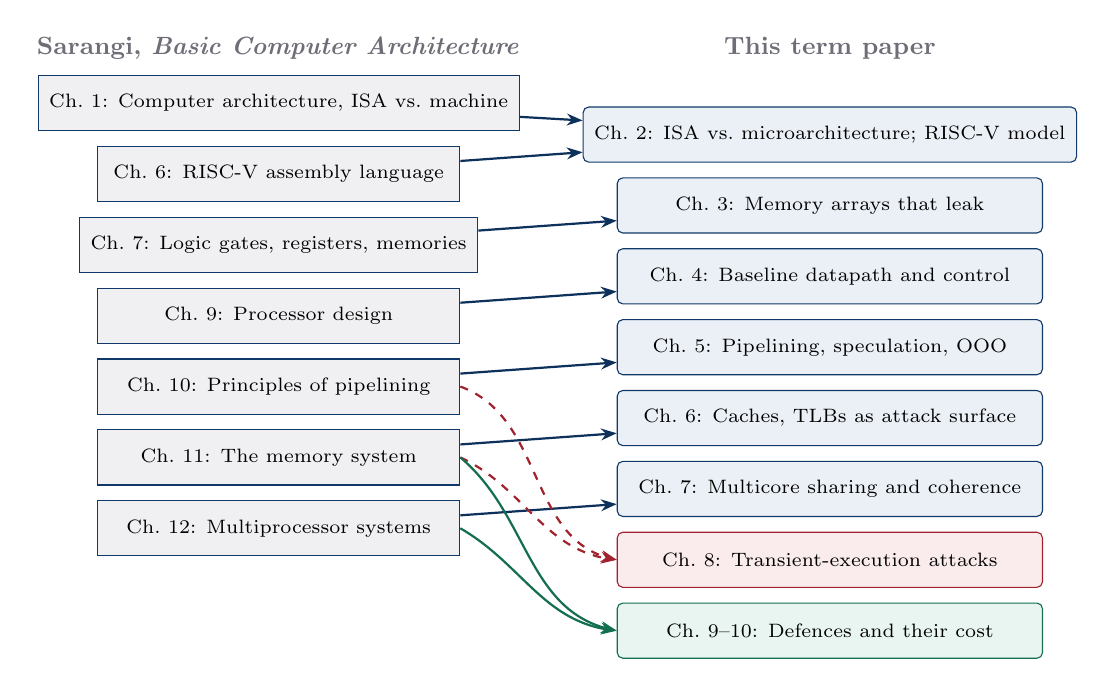
\begin{tikzpicture}[node distance=2mm]
  \tikzset{tb/.style={memblk, minimum width=4.6cm, font=\scriptsize, minimum height=7mm},
           pp/.style={blk, minimum width=5.4cm, font=\scriptsize, minimum height=7mm}}
  % textbook column
  \node[font=\small\bfseries, text=muted] at (-3.4,1.1) {Sarangi, \textit{Basic Computer Architecture}};
  \node[tb] (t1)  at (-3.4, 0.4) {Ch.~1: Computer architecture, ISA vs.\ machine};
  \node[tb] (t6)  at (-3.4,-0.5) {Ch.~6: RISC-V assembly language};
  \node[tb] (t7)  at (-3.4,-1.4) {Ch.~7: Logic gates, registers, memories};
  \node[tb] (t9)  at (-3.4,-2.3) {Ch.~9: Processor design};
  \node[tb] (t10) at (-3.4,-3.2) {Ch.~10: Principles of pipelining};
  \node[tb] (t11) at (-3.4,-4.1) {Ch.~11: The memory system};
  \node[tb] (t12) at (-3.4,-5.0) {Ch.~12: Multiprocessor systems};

  % paper column
  \node[font=\small\bfseries, text=muted] at (3.6,1.1) {This term paper};
  \node[pp] (p2)  at (3.6, 0.0) {Ch.~2: ISA vs.\ \uarch{}; RISC-V model};
  \node[pp] (p3)  at (3.6,-0.9) {Ch.~3: Memory arrays that leak};
  \node[pp] (p4)  at (3.6,-1.8) {Ch.~4: Baseline datapath and control};
  \node[pp] (p5)  at (3.6,-2.7) {Ch.~5: Pipelining, speculation, OOO};
  \node[pp] (p6)  at (3.6,-3.6) {Ch.~6: Caches, TLBs as attack surface};
  \node[pp] (p7)  at (3.6,-4.5) {Ch.~7: Multicore sharing and coherence};
  \node[pp, fill=attackfill, draw=attack] (p8) at (3.6,-5.4) {Ch.~8: Transient-execution attacks};
  \node[pp, fill=defensefill, draw=defense] (p9) at (3.6,-6.3) {Ch.~9--10: Defences and their cost};

  \draw[sig] (t1)  -- (p2);
  \draw[sig] (t6)  -- (p2);
  \draw[sig] (t7)  -- (p3);
  \draw[sig] (t9)  -- (p4);
  \draw[sig] (t10) -- (p5);
  \draw[sig] (t11) -- (p6);
  \draw[sig] (t12) -- (p7);
  \draw[atksig] (t10.east) to[out=-20,in=170] (p8.west);
  \draw[atksig] (t11.east) to[out=-25,in=175] (p8.west);
  \draw[defsig] (t11.east) to[out=-40,in=170] (p9.west);
  \draw[defsig] (t12.east) to[out=-30,in=175] (p9.west);
\end{tikzpicture}
\caption[Textbook-to-paper chapter mapping]{Correspondence between the
prescribed textbook's chapters and the chapters of this paper. Solid arrows
carry background material; dashed red and solid green arrows show where two
textbook chapters (pipelining and the memory system) jointly support the attack
and defence chapters, which have no direct textbook counterpart.}
\label{fig:roadmap}
\end{figure}

\begin{table}[p]
\centering
\caption[Chapter- and section-level textbook mapping]{Chapter- and section-level
mapping between the prescribed textbook~\citep{sarangi2025basic} and this paper.
``Primary'' marks the five chapters that form the spine of the term paper.
Sub-section granularity is given in \Cref{app:tocmap}.}
\label{tab:tocmap}
\footnotesize
\begin{tabularx}{\linewidth}{@{}p{1.7cm}>{\raggedright\arraybackslash}p{2.7cm}p{1.9cm}X@{}}

\toprule
\textbf{Textbook} & \textbf{Sections used} & \textbf{Role} & \textbf{How it is used in this paper} \\
\midrule
Ch.~1 & 1.4, 1.5, 1.7 & Supporting &
The architecture-versus-organization definitions that open the chapter, the
language of instructions, instruction set design, and the design of practical
machines. Used in \Cref{ch:isa} to argue that an open, well-defined
ISA constrains \emph{results} and therefore cannot by itself prevent
implementation-level leakage. \\
\addlinespace
Ch.~6 & 6.1.1--6.1.2, 6.3.1--6.3.3, 6.5 & \textbf{Primary} &
RISC-V base ISAs and extensions; the register view; conditional and
unconditional control transfer; load/store instructions; instruction encoding.
Used in \Cref{ch:isa} for the execution model, for the branch and memory
instructions that drive predictors and caches, and for the encoding space in
which security instructions (barriers, flushes) must be placed. \\
\addlinespace
Ch.~7 & 7.4 (7.4.1--7.4.3) & Supporting &
Memories: static RAM and its arrays, content-addressable memory, and dynamic
RAM. Used in
\Cref{ch:memories} as the physical explanation of why cache, TLB and predictor
accesses have data-dependent latency at all. \\
\addlinespace
Ch.~9 & 9.1, 9.2 (9.2.1--9.2.7), 9.3 & \textbf{Primary} &
Baseline processor: the fetch unit, data path and control path, operand fetch,
execute, memory access, register writeback, the assembled data path, and the
control unit. Used in \Cref{ch:proc} to fix the
reference machine onto which predictors, buffers and caches are later added. \\
\addlinespace
Ch.~10 & 10.1--10.4, 10.8 (10.8.2, 10.8.3), 10.9.3, 10.10 (10.10.2, 10.10.5), 10.11 (10.11.1, 10.11.4) & \textbf{Primary} &
Pipelining; data, control and structural hazards; exceptions and \emph{precise}
exceptions; performance of a non-ideal pipeline; power, dynamic power and the
$ED^{2}$ metric; branch prediction and out-of-order pipelines.
Used in \Cref{ch:pipeline} for speculation and the execution window, in
\Cref{ch:transient} for why precise exceptions do not undo \uarchadj{} effects, and
in \Cref{ch:tradeoffs} for the IPC, power and energy metrics used to price
defences. \\
\addlinespace
Ch.~11 & 11.1.2--11.1.8, 11.2, 11.3 (11.3.1), 11.4 (11.4.2, 11.4.3, 11.4.5, 11.4.6) & \textbf{Primary} &
Locality and the memory hierarchy; caches, their lookup, insertion, replacement
and eviction; the mathematical model of the memory system; virtual memory,
paging, the memory management unit and advanced paging features. Used in \Cref{ch:memsys} for every cache and TLB attack
primitive and for the AMAT-based cost model of flushing and partitioning. \\
\addlinespace
Ch.~12 & 12.2, 12.3, 12.4 (12.4.1--12.4.6, 12.4.8) & \textbf{Primary} &
Software for multiprocessors and Amdahl's law; the multiprocessor design space;
coherence, memory consistency, the physical view of memory, shared caches,
coherent private caches and multithreaded processors. Used in
\Cref{ch:multicore} for cross-core and cross-thread leakage. Cache partitioning
and colouring, used there as \emph{defences}, are not textbook material and are
drawn from the research literature instead. \\
\bottomrule
\end{tabularx}
\end{table}

\section{The gap this paper is about}
\label{sec:gap}

A processor is specified by a contract and built by an optimisation.\index{architecture!versus organization} The
contract, the instruction set architecture or ISA, says what the visible\index{instruction set architecture (ISA)}
state of the machine must be after each instruction retires. The optimisation,
the \uarch{}, decides how to get there quickly: which values to cache, which
branch to guess, which instruction to start before it is known to be needed.\index{microarchitecture}
The contract is written in terms of \emph{values}; the optimisation manipulates
\emph{time}. Two executions that produce the same values are both correct, and
the functional contract does not require them to take the same time.

A structure that speeds up the common case, such as a cache, a\index{side channel!timing}
translation-lookaside buffer or a branch predictor, makes the machine faster
after some events than after others, and the difference is a signal. If the
events depend on secret data, the signal may carry the secret. This mechanism
drives the cache-timing attacks on
AES~\citep{osvik2006cache,bernstein2005aes}, the cross-core attacks on the
last-level cache~\citep{liu2015llc} and the TLB-based leakage of Gras
\etal~\citep{gras2018tlbleed}. Since 2018 it has driven the transient-execution
family as well, in which a processor is induced to compute on data that the\index{transient execution}
program would never have used and to leave a trace of the result in a
cache~\citep{kocher2019spectre,lipp2018meltdown}.

\begin{figure}[t]
\centering
\resizebox{\linewidth}{!}{%
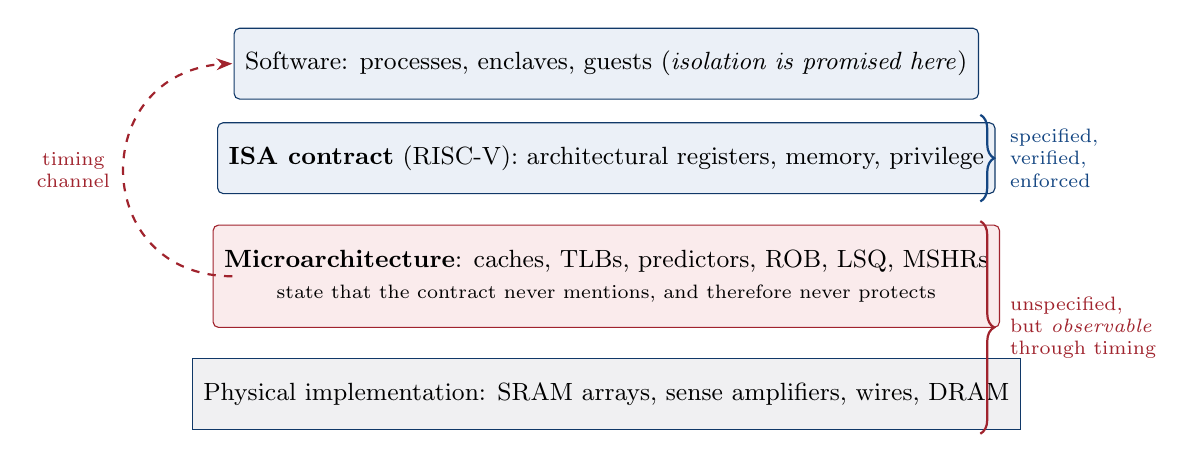
\begin{tikzpicture}[node distance=0mm]
  % Layers
  \node[blk, minimum width=9.2cm, minimum height=9mm] (sw) at (0,3.2)
        {Software: processes, enclaves, guests (\emph{isolation is promised here})};
  \node[blk, minimum width=9.2cm, minimum height=9mm, fill=lightfill] (isa) at (0,2.0)
        {\textbf{ISA contract} (RISC-V): architectural registers, memory, privilege};
  \node[atk, minimum width=9.2cm, minimum height=13mm] (ua) at (0,0.5)
        {\textbf{Microarchitecture}: caches, TLBs, predictors, ROB, LSQ, MSHRs\\
         \scriptsize state that the contract never mentions, and therefore never protects};
  \node[memblk, minimum width=9.2cm, minimum height=9mm] (phys) at (0,-1.0)
        {Physical implementation: SRAM arrays, sense amplifiers, wires, DRAM};

  % Braces / annotations
  \draw[decorate,decoration={brace,amplitude=5pt},thick,accent]
        (4.75,2.55) -- (4.75,1.45) node[midway,right=7pt,align=left,font=\scriptsize]
        {specified,\\verified,\\enforced};
  \draw[decorate,decoration={brace,amplitude=5pt},thick,attack]
        (4.75,1.2) -- (4.75,-1.5) node[midway,right=7pt,align=left,font=\scriptsize,text=attack]
        {unspecified,\\but \emph{observable}\\through timing};

  % leak arrow
  \draw[atksig] (-4.75,0.5) .. controls (-6.6,0.5) and (-6.6,3.2) .. (-4.75,3.2)
        node[midway,left=1pt,font=\scriptsize,text=attack,align=center] {timing\\channel};
\end{tikzpicture}%
}
\caption[The architecture/\uarchadj{} gap]{The gap that this paper studies.
Isolation is promised at the software level and enforced through the ISA
contract, but performance comes from state that lives \emph{below} the contract.
That state is not covered by the isolation promise, yet it is observable from
above through execution time.}
\label{fig:gap}
\end{figure}

\Cref{fig:gap} sets out the problem and fixes the vocabulary used throughout the
paper. Everything above the contract line is what a security argument normally
reasons about; everything below it is what determines how long an instruction
takes. The attacks surveyed in this paper are techniques for making information
cross that line upwards.

\begin{takeaway}
The architectural state of a processor is what the ISA defines. The
\uarchadj{} state is everything else the hardware remembers so that it can be fast.
Confidentiality arguments are usually made about the first; timing attacks
observe the second. A \emph{precise} exception restores architectural state
exactly, and says nothing about \uarchadj{} state: that asymmetry is what
transient-execution attacks rely on.
\end{takeaway}

\section{Why RISC-V specifically}
\label{sec:whyriscv}

Most of the attack literature was developed on x86 and, to a lesser extent, on
Arm. Studying the same phenomena on RISC-V\index{RISC-V!rationale for studying} changes what can be said with
confidence, for four reasons.

\paragraph{The specification is open and layered.} RISC-V separates a small base
integer ISA from optional extensions~\citep{riscv-unpriv} and the unprivileged
ISA from the privileged architecture~\citep{riscv-priv}. It is therefore
possible to say which security property is a property of the
\emph{architecture}, such as the promise of the \texttt{Zkt} extension that
listed instructions execute in data-independent time~\citep{riscv-crypto}, and
which is a property of one \emph{implementation}.

\paragraph{Competitive implementations are open.} Rocket (in-order, five
stages)~\citep{asanovic2016rocket}, BOOM and SonicBOOM (superscalar,
out-of-order)~\citep{celio2015berkeley,zhao2020sonicboom} and CVA6 (six stages,
Linux-capable)~\citep{zaruba2019ariane} are published as RTL that can be read,
modified and simulated. A claimed leak can be traced to a specific queue or
array, and a proposed defence can be implemented and measured.

\paragraph{The attacks are demonstrated, not hypothetical.} Spectre attacks were
replicated on BOOM in cycle-exact simulation in
2019~\citep{gonzalez2019replicating}, and in 2026 on the commercial\index{CVA6 (Ariane) core}
out-of-order processors that are now on sale~\citep{gerlach2026spectre}.
\Cref{ch:transient} keeps these kinds of evidence apart.

\paragraph{The defences are still being decided.} Physical memory protection,
enclave frameworks such as Sanctum~\citep{costan2016sanctum},
MI6~\citep{bourgeat2019mi6} and Keystone~\citep{lee2020keystone}, control-flow
integrity~\citep{riscv-cfi} and temporal
partitioning~\citep{wistoff2021fencet,wistoff2023systematic} are live design
questions, so a paper written now engages with an open design space.

\section{Prior surveys, and the origins of the field}
\label{sec:related}

The study of timing leakage is older than the \uarchadj{} attacks. Kocher showed
in 1996 that key-dependent execution time in implementations of RSA and
Diffie--Hellman suffices to recover secret
exponents~\citep{kocher1996timing}; the target there was the algorithm. The
move to \uarchadj{} targets came with Percival's demonstration that cache
contention on a multithreaded processor leaks across
threads~\citep{percival2005cache} and with the AES cache-timing attacks of
Bernstein~\citep{bernstein2005aes} and of Osvik, Shamir and
Tromer~\citep{osvik2006cache}, which established the eviction and reload
primitives still in use.

Three surveys map the resulting literature. Ge \etal~\citep{ge2018survey} give
a systematic account of \uarchadj{} timing attacks and countermeasures organised
by structure; Canella \etal~\citep{canella2019systematic} systematise
transient-execution attacks and defences with a classification tree; and Xiong
and Szefer~\citep{xiong2021survey} survey transient-execution attacks together
with their mitigations. This paper differs from all three in scope and in
intent. It is confined to RISC-V, it is organised around a single prescribed
textbook, and it adds a model study in which several defence classes are
priced on one baseline. Where a general reference on quantitative processor
design is needed beyond the prescribed text, Hennessy and
Patterson~\citep{hennessy2019quantitative} is used as a secondary source.

\section{Research questions}
\label{sec:rqs}

The paper is organised around five questions.

\begin{enumerate}[label=\textbf{RQ\arabic*.}, leftmargin=2.4em]
  \item \textbf{Where does the state live?} Which \uarchadj{} structures of a
        RISC-V core retain information across a privilege or process boundary,
        and at what granularity?
        (\Cref{ch:memories,ch:proc,ch:pipeline,ch:memsys,ch:multicore}.)
  \item \textbf{How is it read out?} What is the measurement, what does the
        observer need to share with the victim, and how reliable is one
        observation? (\Cref{ch:memsys,ch:multicore}, \Cref{app:leakage}.)
  \item \textbf{What does speculation add?} How much work can a core do on a
        wrong path, and which of that work changes state that outlives the
        squash? (\Cref{ch:pipeline,ch:transient}.)
  \item \textbf{What do defences do?} Under a common taxonomy, what does each
        class remove and what does it leave? (\Cref{ch:defenses}.)
  \item \textbf{What does security cost?} What do the defences cost in the
        published evaluations, why are those numbers not comparable, and what
        do representative mechanisms cost when they are applied to one and the
        same baseline? (\Cref{ch:tradeoffs,ch:study}.)
\end{enumerate}

\section{Scope and non-goals}

\textbf{In scope.} Timing-based \uarchadj{} leakage in single-core and multicore
RISC-V processors: data and instruction caches, the TLB and page-walk hardware,
branch prediction structures, the store buffer and load-store queue, the
coherence fabric and the shared last-level cache; the transient-execution
families that use those structures; and hardware, ISA-level and software
defences with their costs.

\textbf{Out of scope}, to keep the paper coherent: physical side channels that
need instrumentation (power, electromagnetic, acoustic); fault injection and
disturbance attacks such as Rowhammer~\citep{kim2014rowhammer}, which corrupt
state instead of reading it; weaknesses of cryptographic protocols; and
software memory-safety errors, except where they interact with speculation.
No attack program is developed or run in this paper. The practical part
measures the behaviour of \emph{benign} programs on a model, and what defences
cost.

\section{Method}
\label{sec:method}

The paper combines a literature survey with a model study, and the two answer
different questions.

\textbf{The survey} draws on four kinds of source, which are kept apart in the\index{evidence!classes of}
text: the prescribed textbook, for background; the RISC-V specifications, for
what the architecture does and does not guarantee; peer-reviewed papers, for
attacks, defences and their measured costs; and technical reports, preprints
and project documentation, used where no reviewed source exists and marked as
such in the Bibliography. A published number is always quoted with the platform
on which it was obtained, because \Cref{sec:incomparable} shows that the
platform matters as much as the mechanism. For RISC-V the survey separates
results on silicon, results in cycle-exact RTL simulation, and expectations
derived by analogy with other architectures.

\textbf{The model study} supplies numbers that the literature cannot: the cost\index{model study!purpose}
of several defence classes on a single baseline, with everything else held
constant. Its instrument is a trace-driven timing model in the tradition of
first-order superscalar
models~\citep{karkhanis2004first,eyerman2009mechanistic}; it is specified in
\Cref{app:model}, validated in \Cref{app:validation} and described in
\Cref{ch:study}. Its results are trends on a stated model. They are not
measurements of a RISC-V chip, and the text never presents them as such.

\section{Contributions}

\begin{enumerate}[leftmargin=1.8em]
  \item \textbf{A bottom-up construction that follows the syllabus.} The
        machine is built in textbook order, and the information each structure
        retains is identified at the point where the structure is introduced.
  \item \textbf{A RISC-V evidence table} that separates silicon, RTL
        simulation and inference, including the 2026 results on commercial
        cores (\Cref{tab:rvevidence}).
  \item \textbf{A defence taxonomy with coverage and residual risk}
        (\Cref{tab:coverage,tab:defenses}), and a table of published costs with
        the baseline of each (\Cref{tab:reported}).
  \item \textbf{A reproducible model study.} A simulator, an assembler and
        eleven kernels, cross-checked against QEMU, with which seven
        speculation defences and five isolation mechanisms are priced on one
        baseline and their residual transient footprint is counted
        (\Cref{ch:study}).
  \item \textbf{Three findings from that study}: defence cost rises with the
        aggressiveness of the baseline; the cost of isolation is governed by
        the distance of the working set from the capacity that remains, not by
        the mechanism; and the costs of an isolation mechanism and a
        speculation defence combine roughly multiplicatively
        (\Cref{ch:tradeoffs,ch:study}).
\end{enumerate}

\section{Organisation, and the role of the appendices}

\Cref{ch:isa} establishes the distinction between architecture and \uarch{},
the RISC-V execution model and the threat model. \Cref{ch:memories} descends to
the memory arrays, \Cref{ch:proc} fixes the reference datapath, and
\Cref{ch:pipeline} adds pipelining, prediction and out-of-order execution.
\Cref{ch:memsys} treats the memory hierarchy and \Cref{ch:multicore} multicore
sharing. \Cref{ch:transient} covers transient execution, \Cref{ch:defenses} the
defences and \Cref{ch:tradeoffs} their cost. \Cref{ch:study} documents the model
study and \Cref{ch:conclusion} concludes.

The course guideline asks that any explanation longer than half a page be moved\index{appendices!role of}
to an appendix of its own. The chapters therefore carry the argument, the
figures and the results, and each derivation, worked example or mechanism
description that needs more room has its own appendix, to which the chapter
points. \Cref{app:plagiarism,app:readability} are the plagiarism report and the
reading indices; \Cref{app:metrics,app:tocmap} hold the cost metrics and the
detailed textbook mapping; \Cref{app:leakage} to \Cref{app:specdef} are the
extended explanations; \Cref{app:model} to \Cref{app:source} document the model
study, its validation, its complete results and its programs; and
\Cref{app:toolchain} describes the build and checks the submission against the
guidelines.

\begin{tocmapbox}
A box like this one opens each technical chapter and names the textbook sections
that supply its background, so that the correspondence of \Cref{tab:tocmap} can
be checked at the point of use.
\end{tocmapbox}


\chapter{The Contract and the Machine: RISC-V as Architecture and as Implementation}
\label{ch:isa}

\begin{tocmapbox}
Background: textbook Chapter~1, which defines \emph{architecture} as the view of
a computer presented to software designers and \emph{organization} as its
hardware implementation, with \SecRef{1.4} (the language of instructions),
\SecRef{1.5} (instruction set design) and \SecRef{1.7} (design of practical
machines); and Chapter~6, \SecRef{6.1.1} (RISC-V base ISAs and extensions),
\SecRef{6.1.2} (view of registers), \SecRef{6.3.1}--\SecRef{6.3.3} (branches,
loads and stores) and \SecRef{6.5} (instruction
encoding)~\citep{sarangi2025basic}.
\end{tocmapbox}

\section{An ISA is a contract about values}
\label{sec:contract}

The textbook opens with the distinction on which this paper depends: the
\emph{architecture} is the view of a computer presented to software designers,
the \emph{organization} is its implementation in hardware. Two implementations
of one ISA must agree on the value written into every architectural register
and memory location. They need not agree on pipeline depth, issue width, cache
sizes, predictor organisation or replacement policy, and in practice they do
not.

To state the contract, restrict attention to a single hart running a
deterministic program without interrupts. Let $A$ be the architectural state:\index{architectural state}
the integer registers, the program counter, the control and status registers
visible at the current privilege level, and memory. Let $\mu$ be the
\uarchadj{} state: cache contents and replacement metadata, TLB entries, branch\index{microarchitectural state}
history and target tables, the reorder buffer, the load-store queue, miss-status
holding registers, fill and store buffers, prefetcher tables. An implementation
is \emph{functionally correct} if, for every such program $P$ and initial state
$A_0$, the sequence of architectural states at instruction boundaries is the
one the ISA specifies:
\begin{equation}
  \mathrm{exec}(P, A_0) \;=\; A_0, A_1, A_2, \ldots
  \label{eq:contract}
\end{equation}
\Cref{eq:contract} does not mention $\mu$, and it does not mention the number of
cycles between $A_i$ and $A_{i+1}$. A functionally correct implementation may
therefore let $\mu$ depend on secret data and let execution time depend on
$\mu$. Composing the two dependences gives a channel from secret data to time.

The base contract is silent about time, but RISC-V is not entirely so. The
\texttt{Zkt} extension is a timing clause: it lists instructions whose latency
must not depend on their data operands~\citep{riscv-crypto}. Counters such as
\code{cycle} and \code{time} are architectural state too, which is why
\Cref{eq:contract} is stated for a restricted model: a program that reads the
cycle counter observes $\mu$ through an architectural register.

\begin{takeaway}
The attacks in this paper follow one pattern: find a computation whose effect on
$\mu$ depends on a secret, and a way to convert $\mu$ back into time. The
functional contract of the ISA is not violated at any point, so functional
correctness cannot rule these channels out. Ruling them out needs a contract
that speaks about time or about $\mu$, and \Cref{sec:leakmodel} sketches what
such a contract looks like.
\end{takeaway}

\section{The RISC-V execution model}

\subsection{Base ISAs and extensions}

RISC-V is defined as a small base integer instruction set plus optional standard
extensions~\citep{riscv-unpriv}. The base is RV32I or RV64I; extensions add\index{RISC-V!base integer ISA}
multiplication and division (M), atomics (A), floating point (F, D),
compressed encodings (C), vectors (V), bit manipulation (B) and cryptography\index{RISC-V!standard extensions}
(K). The shorthand \texttt{RV64GC} denotes RV64IMAFDC. The kernels of
\Cref{ch:study} use RV64IM only.

Each extension is a set of promises about \emph{results}; very few make a
promise about \emph{timing} or about \uarchadj{} state. \Cref{tab:extensions}
lists the features that bear on this paper and states what each does and does
not guarantee.

\begin{table}[t]
\centering
\caption[RISC-V features relevant to \uarchadj{} security]{RISC-V architectural
features that bear on \uarchadj{} security, and the limits of what each
guarantees.}
\label{tab:extensions}
\footnotesize
\begin{tabularx}{\linewidth}{@{}>{\raggedright\arraybackslash}p{2.6cm}>{\raggedright\arraybackslash}p{4.1cm}X@{}}
\toprule
\textbf{Feature} & \textbf{What it provides} & \textbf{What it does \emph{not} provide} \\
\midrule
PMP &
Access control over physical address ranges, set by machine
mode~\citep{riscv-priv}. &
Any statement about whether a denied access has already changed a cache or a
predictor; the check is architectural. \\
\addlinespace
Sv39 / Sv48 paging &
Virtual memory, per-page permissions, address-space identifiers in
\code{satp}~\citep{riscv-priv}. &
Any statement about TLB residency, page-walk caching or the duration of a walk. \\
\addlinespace
\texttt{Zkt} &
Latency independent of data operands for a listed set of
instructions~\citep{riscv-crypto}. &
Coverage of loads, stores and conditional branches, which are not in the list;
address-dependent timing is therefore outside it. \\
\addlinespace
\texttt{Zicfilp}, \texttt{Zicfiss} &
Landing pads and a shadow stack for control-flow integrity~\citep{riscv-cfi}. &
A guarantee about transient execution. The specification notes that an
implementation may apply the landing-pad check to speculative targets as well,
which narrows what branch-target injection can reach; that is a property of the
implementation. \\
\addlinespace
\texttt{fence}, \texttt{fence.i}, \texttt{sfence.vma} &
Ordering of memory accesses, synchronisation of instruction fetch,
invalidation of cached translations~\citep{riscv-unpriv,riscv-priv}. &
Erasure or a speculation barrier. A \texttt{fence} orders memory operations; it
is not specified to remove cache lines or to stop speculative execution. \\
\addlinespace
\texttt{fence.t} \newline (proposed) &
A temporal fence that clears on-core \uarchadj{} state at a domain switch,
implemented on CVA6~\citep{wistoff2021fencet,wistoff2023systematic}. &
Ratified status; coverage of state outside the core, which has to be
partitioned separately. \\
\addlinespace
\texttt{cbo.flush}, \texttt{cbo.inval} (Zicbom) &
Cache-block management by address~\citep{riscv-cmo}. &
Neutrality: flushing a chosen block is also the eviction step of Flush+Reload.
Execution from lower privilege levels is controlled by the environment
configuration registers. \\
\bottomrule
\end{tabularx}
\end{table}

The last row deserves emphasis. Cache-block management was added for\index{cache management instructions (Zicbom)}
correctness with devices that bypass the cache and for performance. Where user
mode is allowed to execute it, the same instruction also gives an observer a
precise way to evict a chosen line\index{Flush+Reload}. A feature at one layer is a measuring
tool at another, and this tension recurs throughout the paper.

\subsection{Registers, branches, loads and stores}
\label{sec:ctrlmem}

RV64I provides 32 integer registers \code{x0}--\code{x31}, with \code{x0}
hardwired to zero, and the program counter. Registers are architectural state:
at a context switch the operating system saves and restores them, so one
context cannot read what another left there. No instruction saves or restores\index{context switch!state not covered by the ISA}
the branch history, and the ISA does not require a context switch to clear it.

Two instruction classes drive the structures this paper is concerned with.
\textbf{Conditional branches} (\code{beq}, \code{bne}, \code{blt}, \code{bge},
\code{bltu}, \code{bgeu}) and the \textbf{jumps} \code{jal} and \code{jalr}
train the direction predictor, the branch target buffer and the\index{branch target buffer (BTB)}
return-address stack.\index{return address stack (RAS)} \textbf{Loads and stores} compute an effective address
as a base register plus a 12-bit immediate.\index{load and store instructions!effective address} The address is data-dependent
whenever the base register holds a value derived from data, as in every table
lookup, and the latency of the access depends on where the line is found.
\Cref{lst:leak} shows the pattern in its smallest form.

\begin{lstlisting}[language=riscv, caption={The canonical leak, in RISC-V. The
address of the second load depends on a secret byte; its latency therefore
reveals which line was touched. Nothing here violates the ISA.},
label={lst:leak}]
# a0 = pointer to secret byte, a1 = base of a 256*64-byte probe array
  lbu   t0, 0(a0)        # t0 = secret byte  (0..255)
  slli  t0, t0, 6        # t0 = secret * 64  (one cache line per value)
  add   t1, a1, t0       # address depends on the secret
  lbu   t2, 0(t1)        # this access installs ONE line of the probe array
# ...the value in t2 is never used; the *state change* is the message.
\end{lstlisting}

Architecturally the sequence computes a value in \code{t2} and nothing else. In
terms of $\mu$ it installs one particular line of the table in the cache, and
which line depends on the byte that was loaded first. If the sequence is later
squashed, the architectural effect is nil, and what happens to the installed
line is up to the implementation.

\subsection{Instruction encoding}

\Cref{fig:encoding} shows the six base instruction formats. Source register
fields sit at fixed positions in every format so that the register file can be\index{RISC-V!instruction encoding}
read before decoding completes~\citep{riscv-unpriv}: a small example of the
theme of textbook \SecRef{1.7}, that the practical machine shapes the
specification. The encoding also bounds what a defence can ask for. A new
instruction such as \code{fence.t} consumes encoding space and needs control
registers, which is one reason why many hardware defences in
\Cref{ch:defenses} are designed to be transparent to the ISA.

\begin{figure}[t]
\centering
\resizebox{\linewidth}{!}{%
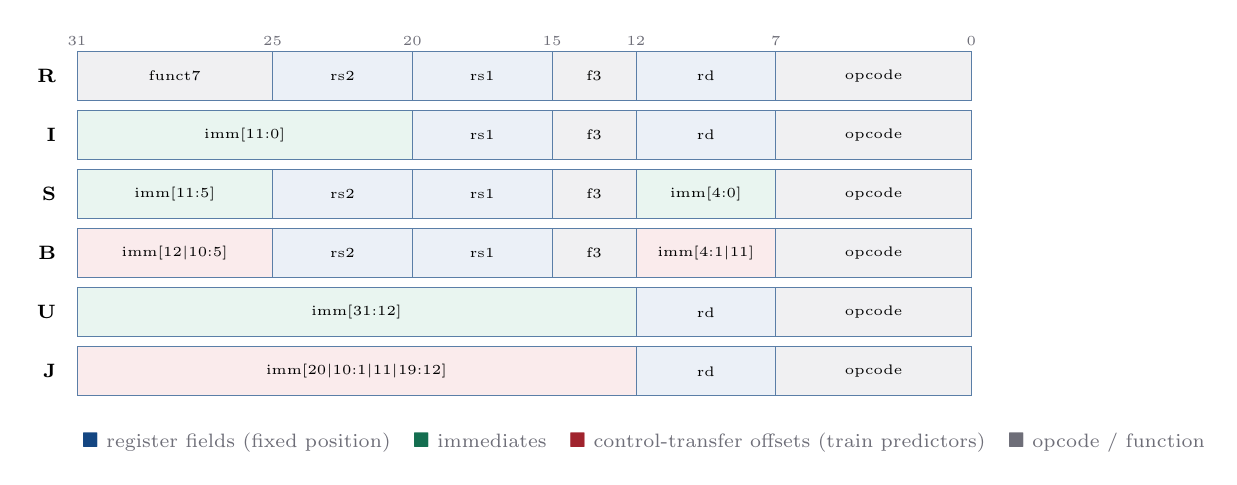
\begin{tikzpicture}[x=3.55mm, y=1cm]
  \newcommand{\fld}[5]{%
    \draw[fill=#5, draw=accent!70, line width=0.3pt] (#1,#2) rectangle ++(#3,0.62);
    \node[font=\tiny] at ({#1+#3/2}, {#2+0.31}) {#4};}
  % bit ruler
  \foreach \b/\x in {31/0, 25/7, 20/12, 15/17, 12/20, 7/25, 0/32}
     {\node[font=\tiny, text=muted] at (\x,4.85) {\b};}
  % R-type  (y=4.1)
  \node[font=\scriptsize\bfseries, anchor=east] at (-0.4,4.41) {R};
  \fld{0}{4.1}{7}{funct7}{greyfill}\fld{7}{4.1}{5}{rs2}{lightfill}
  \fld{12}{4.1}{5}{rs1}{lightfill}\fld{17}{4.1}{3}{f3}{greyfill}
  \fld{20}{4.1}{5}{rd}{lightfill}\fld{25}{4.1}{7}{opcode}{greyfill}
  % I-type (y=3.35)
  \node[font=\scriptsize\bfseries, anchor=east] at (-0.4,3.66) {I};
  \fld{0}{3.35}{12}{imm[11:0]}{defensefill}\fld{12}{3.35}{5}{rs1}{lightfill}
  \fld{17}{3.35}{3}{f3}{greyfill}\fld{20}{3.35}{5}{rd}{lightfill}
  \fld{25}{3.35}{7}{opcode}{greyfill}
  % S-type (y=2.6)
  \node[font=\scriptsize\bfseries, anchor=east] at (-0.4,2.91) {S};
  \fld{0}{2.6}{7}{imm[11:5]}{defensefill}\fld{7}{2.6}{5}{rs2}{lightfill}
  \fld{12}{2.6}{5}{rs1}{lightfill}\fld{17}{2.6}{3}{f3}{greyfill}
  \fld{20}{2.6}{5}{imm[4:0]}{defensefill}\fld{25}{2.6}{7}{opcode}{greyfill}
  % B-type (y=1.85)
  \node[font=\scriptsize\bfseries, anchor=east] at (-0.4,2.16) {B};
  \fld{0}{1.85}{7}{imm[12$|$10:5]}{attackfill}\fld{7}{1.85}{5}{rs2}{lightfill}
  \fld{12}{1.85}{5}{rs1}{lightfill}\fld{17}{1.85}{3}{f3}{greyfill}
  \fld{20}{1.85}{5}{imm[4:1$|$11]}{attackfill}\fld{25}{1.85}{7}{opcode}{greyfill}
  % U-type (y=1.1)
  \node[font=\scriptsize\bfseries, anchor=east] at (-0.4,1.41) {U};
  \fld{0}{1.1}{20}{imm[31:12]}{defensefill}\fld{20}{1.1}{5}{rd}{lightfill}
  \fld{25}{1.1}{7}{opcode}{greyfill}
  % J-type (y=0.35)
  \node[font=\scriptsize\bfseries, anchor=east] at (-0.4,0.66) {J};
  \fld{0}{0.35}{20}{imm[20$|$10:1$|$11$|$19:12]}{attackfill}\fld{20}{0.35}{5}{rd}{lightfill}
  \fld{25}{0.35}{7}{opcode}{greyfill}
  % legend
  \node[note, anchor=west] at (0,-0.25)
    {\textcolor{accent}{$\blacksquare$}~register fields (fixed position)\quad
     \textcolor{defense}{$\blacksquare$}~immediates\quad
     \textcolor{attack}{$\blacksquare$}~control-transfer offsets (train predictors)\quad
     $\blacksquare$~opcode / function};
\end{tikzpicture}%
}
\caption[RISC-V base instruction formats]{The six base RISC-V instruction
formats, drawn to bit scale (textbook \SecRef{6.5}). The \code{rs1}, \code{rs2}
and \code{rd} fields occupy the same bit positions in every format, so the
register file can be read speculatively during decode, a \uarch{}
optimisation visible in the architecture. The B- and J-type offsets (red) are
what train the direction predictor, the branch target buffer and the
return-address stack; the I- and S-type immediates feed effective-address
computation and therefore the cache.}
\label{fig:encoding}
\end{figure}

\section{The privileged architecture in brief}
\label{sec:privbrief}

Three parts of the privileged architecture~\citep{riscv-priv} recur in later
chapters; \Cref{app:priv} walks through each with a worked example.

\textbf{Privilege modes and traps.} Code runs in machine (M), supervisor (S) or\index{privilege modes}
user (U) mode. A trap saves the program counter in \code{mepc} or \code{sepc},
records the cause, and transfers control to the handler; the trap is precise.
The mode switch changes which architectural state is accessible. It does not
change the contents of caches or predictors.

\textbf{Physical memory protection.} PMP entries let machine mode grant or deny\index{physical memory protection (PMP)}
read, write and execute access to ranges of physical addresses for S and U
mode. The check decides whether an access \emph{faults}. When, relative to the
check, the data of a faulting load becomes available to later instructions is
not specified.

\textbf{Paging and address-space identifiers.} Under Sv39 a virtual address is\index{paging!Sv39 and Sv48}
translated by a three-level page-table walk rooted at the page number held in
\code{satp}. The same register holds an address-space identifier (ASID), which\index{address-space identifier (ASID)}
lets a TLB keep the translations of several address spaces at once, so that a
context switch need not flush it; \code{sfence.vma} invalidates entries when
the operating system changes a mapping or reuses an identifier.

\section{Architectural versus microarchitectural state}
\label{sec:archvsuarch}

\Cref{tab:statepartition} partitions the state of a representative out-of-order
RISC-V core. The criterion is operational: state is architectural if a correct
implementation and operating system must save and restore it across an
exception or a context switch, and \uarchadj{} if they need not. The third
column says what the ISA requires; what a particular core and kernel do in
addition is their own choice, and \Cref{ch:defenses} is about those choices.

\begin{table}[t]
\centering
\caption[Partition of processor state]{Partition of the state of a
representative out-of-order RISC-V core. The last column gives the granularity
at which an observation of the structure resolves the activity of another
context.}
\label{tab:statepartition}
\footnotesize
\begin{tabularx}{\linewidth}{@{}>{\raggedright\arraybackslash}p{3.4cm}>{\raggedright\arraybackslash}p{2.15cm}>{\raggedright\arraybackslash}X>{\raggedright\arraybackslash}p{2.5cm}@{}}
\toprule
\textbf{Structure} & \textbf{Class} & \textbf{At a context switch, the ISA requires} & \textbf{Granularity} \\
\midrule
\code{x0}--\code{x31}, PC, CSRs & Architectural & Save and restore, by the OS & not a channel \\
Memory, page tables            & Architectural & Protection by PMP and paging & not a channel \\
\midrule
L1, L2 and last-level cache data & Microarch. & Nothing & Cache line (\SI{64}{\byte}) \\
Cache replacement metadata       & Microarch. & Nothing & Way within a set \\
TLB, page-walk caches            & Microarch. & Nothing if ASIDs differ; invalidation when an ASID is reused & Page (\SI{4}{\kibi\byte}) \\
Branch direction predictor       & Microarch. & Nothing & One outcome per branch \\
Branch target buffer             & Microarch. & Nothing & Target address bits \\
Return address stack             & Microarch. & Nothing & Call depth and target \\
Reorder buffer, issue queues     & Microarch. & Nothing (drained by the trap) & Occupancy, timing \\
Store buffer, load-store queue   & Microarch. & Nothing (drained by the trap) & Address match \\
MSHRs, fill buffers              & Microarch. & Nothing & Line in flight \\
Prefetcher tables                & Microarch. & Nothing & Access stride \\
DRAM row buffers (\SecRef{7.4.3}) & Microarch. & Nothing & DRAM row \\
\bottomrule
\end{tabularx}
\end{table}

Two rows deserve a second look. The reorder buffer is drained at a trap, so its
contents do not survive, but its occupancy affects the timing of the
instructions that follow. And the TLB row shows a performance feature with a
security side: ASID tagging exists precisely so that translations of another
address space may stay resident.

\section{Threat model}
\label{sec:threat}

A leakage claim means nothing without a statement of who observes.\index{threat model} This paper
uses the four scenarios of \Cref{tab:threat}. They are not ordered by strength:
a sandboxed script shares more hardware with its victim than an unprivileged
process on another core, but can execute less. Each attack discussed later is
labelled with the scenarios in which it has been shown to work.

\begin{table}[t]
\centering
\caption[Attacker scenarios]{The four attacker scenarios used in this paper,
described by what the attacker can execute, what hardware it shares with the
victim, and when it runs.}
\label{tab:threat}
\footnotesize
\begin{tabularx}{\linewidth}{@{}p{0.5cm}>{\raggedright\arraybackslash}p{2.9cm}>{\raggedright\arraybackslash}p{3.3cm}X@{}}
\toprule
 & \textbf{Scenario} & \textbf{Code the attacker runs} & \textbf{Hardware shared with the victim} \\
\midrule
S1 & Same address space &
Sandboxed code inside the victim's process (script engine, in-kernel
bytecode, plug-in) &
Everything: address space, core, all caches and predictors. Isolation is a
software policy such as a bounds check. \\
\addlinespace
S2 & Same core, other process or privilege level &
An ordinary unprivileged process &
The core's caches, TLB and predictors, in alternation; simultaneously if the
core is multithreaded. \\
\addlinespace
S3 & Other core, same package &
An ordinary unprivileged process, running concurrently &
The last-level cache, the interconnect, the memory controller and DRAM. The
setting of cloud co-tenancy~\citep{liu2015llc}. \\
\addlinespace
S4 & Remote &
None on the victim machine &
Nothing directly; the attacker observes response times over a network. \\
\bottomrule
\end{tabularx}
\end{table}

\textbf{Common assumptions.} The attacker knows the \uarch{} in detail, which
is trivially true for open cores. The attacker has a timing source: the
\code{cycle} or \code{time} counter where the counter-enable registers permit
it, a counting thread otherwise. The attacker cannot mount physical attacks or
induce faults, and the cryptography is assumed correct, so that any key
recovery is attributable to the \uarch{} and not to the algorithm.

\section{A leakage model in brief}
\label{sec:leakmodel}

Let a victim computation take a secret $s$, a public input $p$ and inputs $a$\index{leakage model}
chosen by the attacker, and let $O$ be what the attacker observes: a vector of
measured latencies. The implementation is \emph{non-interferent} for this\index{non-interference}
victim if the distribution of $O$ is the same for every pair of secrets,
\begin{equation}
  \Pr[\,O \mid p, a, s\,] \;=\; \Pr[\,O \mid p, a, s'\,] \qquad \text{for all } s, s'.
  \label{eq:ni}
\end{equation}
When \Cref{eq:ni} fails, the amount learned from one observation is bounded by
the mutual information $I(S;O \mid P,A)$, and the rate at which a channel can
be used reliably is bounded by its capacity. For the simplest case, a single
hit-or-miss observation that is misclassified with probability $\varepsilon$,
the channel is a binary symmetric channel with capacity\index{channel capacity}
\begin{equation}
  C \;=\; 1 - H_2(\varepsilon), \qquad
  H_2(\varepsilon) = -\varepsilon\log_2\varepsilon - (1-\varepsilon)\log_2(1-\varepsilon)
  \label{eq:bsc}
\end{equation}
bits per observation~\citep{cover2006elements}. \Cref{app:leakage} develops the
model: how $\varepsilon$ follows from the separation of the hit and miss
latencies and the noise of the timer, how many repetitions a given reliability
needs, and why capacity is an upper bound and not an attack bandwidth.

Two consequences are used later. \emph{Constant-time programming} is the\index{constant-time code}
discipline of writing the victim so that its branch outcomes and memory
addresses do not depend on $s$; it removes the dependence of $\mu$ on the secret
for committed instructions and says nothing about transient ones. A
\emph{hardware-software contract}~\citep{guarnieri2021hardware} states the\index{hardware-software contract}
other half: which observations the hardware may expose, for committed and for
transient execution, so that software written to the discipline is in fact
non-interferent. The defences of \Cref{ch:defenses} can be read as hardware
that satisfies stronger or weaker contracts of this kind.


\chapter{The Physical Substrate: Memory Arrays That Remember}
\label{ch:memories}

\begin{tocmapbox}
Background: textbook \SecRef{7.4} (memories) with \SecRef{7.4.1} (static RAM),
\SecRef{7.4.2} (content-addressable memory) and \SecRef{7.4.3} (dynamic
RAM)~\citep{sarangi2025basic}.
\end{tocmapbox}

\section{Why a security paper goes down to the array}

Cache attacks can be described purely in terms of hits and misses, and most
surveys do so. That abstraction hides where the latency difference comes from
and why it cannot simply be engineered away. Every structure that later
chapters treat as a channel, whether cache, TLB, branch target buffer or
predictor table, is an array of storage cells with a lookup wrapped around it.
This chapter describes that array once. The quantitative argument, a
first-order model of how access time grows with array size, is in
\Cref{app:arraymodel}.

\section{The storage cell}

\Cref{fig:sram} shows the six-transistor SRAM cell: two cross-coupled\index{SRAM!six-transistor cell}
inverters holding a bit, and two access transistors that connect the internal
nodes to a pair of bit lines when the word line is asserted.

\begin{figure}[t]
\centering
\begin{circuitikz}[scale=0.95, transform shape]
  % --- storage core: two cross-coupled inverters -------------------
  \draw (0,0.75)  node[not port](I1){};
  \draw (0,-0.75) node[not port, rotate=180](I2){};
  \draw (I1.out) -- (1.1,0.75) -- (1.1,-0.75) -- (I2.in);
  \draw (I2.out) -- (-1.1,-0.75) -- (-1.1,0.75) -- (I1.in);
  \node[font=\scriptsize, right] at (1.15,0.15) {$\overline{Q}$};
  \node[font=\scriptsize, left]  at (-1.15,0.15) {$Q$};

  % --- access transistors ------------------------------------------
  \draw (-2.0,0) node[nmos, rotate=-90](AL){};
  \draw ( 2.0,0) node[nmos, rotate=-90](AR){};
  \draw (AL.drain) -- (-1.1,0);   \filldraw (-1.1,0) circle (1.3pt);
  \draw (AR.source) -- (1.1,0);   \filldraw ( 1.1,0) circle (1.3pt);
  \draw (AL.source) -- (-3.0,0);
  \draw (AR.drain)  -- ( 3.0,0);

  % --- word line ----------------------------------------------------
  \draw[accent, thick] (-3.6,1.9) -- (3.6,1.9)
        node[right, font=\scriptsize, black] {WL};
  \draw (AL.gate) -- (-2.0,1.9); \filldraw (-2.0,1.9) circle (1.3pt);
  \draw (AR.gate) -- ( 2.0,1.9); \filldraw ( 2.0,1.9) circle (1.3pt);

  % --- bit lines ----------------------------------------------------
  \draw[accent, thick] (-3.0,-2.3) -- (-3.0,2.7) node[above, font=\scriptsize, black] {BL};
  \draw[accent, thick] ( 3.0,-2.3) -- ( 3.0,2.7) node[above, font=\scriptsize, black] {$\overline{\text{BL}}$};

  % --- precharge and sense amp blocks -------------------------------
  \node[memblk, font=\scriptsize, minimum width=2.4cm, minimum height=6mm] (pc) at (0,2.7)
        {precharge / equalise};
  \draw (pc.west) -- (-3.0,2.7);  \draw (pc.east) -- (3.0,2.7);
  \node[memblk, font=\scriptsize, minimum width=2.4cm, minimum height=6mm] (sa) at (0,-2.3)
        {sense amplifier};
  \draw (sa.west) -- (-3.0,-2.3); \draw (sa.east) -- (3.0,-2.3);
  \draw[sig] (sa.south) -- ++(0,-0.6) node[below, font=\scriptsize] {data out};

  % --- annotations ---------------------------------------------------
  \node[note, anchor=west, text width=4.1cm] at (3.9,0.4)
        {The cell can only pull the bit lines apart slowly: it is sized to be
         \emph{small}, not strong. The delay from WL rising to a resolvable
         $\Delta V$ is the irreducible core of access latency.};
\end{circuitikz}
\caption[Six-transistor SRAM cell]{The 6T SRAM cell (textbook \SecRef{7.4.1}).
Two cross-coupled inverters store the bit; two access transistors couple it to a
precharged differential bit-line pair when the word line is asserted. Reading is
destructive-by-degree: the cell must discharge a large bit-line capacitance
through a deliberately weak transistor, which is why an array access costs
hundreds of picoseconds to nanoseconds rather than a gate delay.}
\label{fig:sram}
\end{figure}

Two design pressures shape the cell. It is made as small as possible, so its
transistors are weak and the bit-line swing develops slowly; a sense amplifier
is needed, and sensing has to be timed. And the bit lines are shared down a
whole column, so their capacitance grows with the number of rows. A small array
can therefore be read within a clock cycle and a large one cannot, and the
designer of a memory hierarchy chooses the sizes with exactly this in mind.

\section{From cell to array}

\Cref{fig:array} shows the organisation of textbook \SecRef{7.4.1}: a decoder
turns an address into one asserted word line, a two-dimensional cell array
holds the data, sense amplifiers convert small differential voltages into logic
levels, and a column multiplexer selects the bits required.
\Cref{fig:readtiming} shows the same access in time.

\begin{figure}[t]
\centering
\resizebox{\linewidth}{!}{%
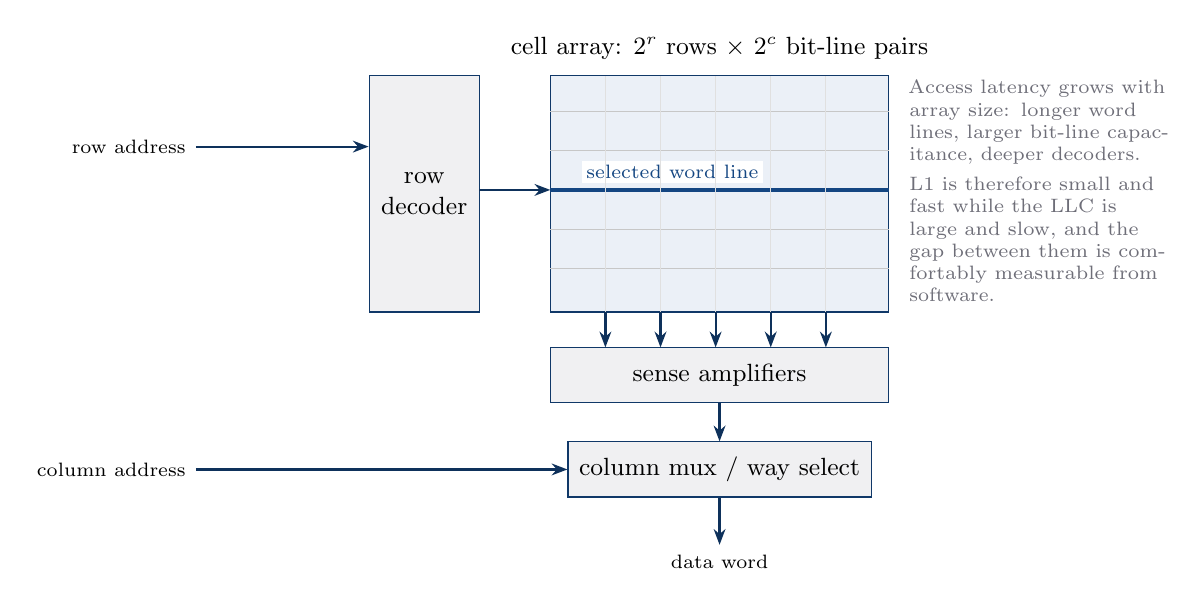
\begin{tikzpicture}[scale=1.0]
  % --- decoder -------------------------------------------------------
  \node[memblk, minimum width=1.4cm, minimum height=3.0cm, align=center] (dec) at (0,0)
        {row\\decoder};
  % --- array box -----------------------------------------------------
  \draw[draw=accent!80!black, fill=lightfill] (1.6,-1.5) rectangle (5.9,1.5);
  \node[font=\small] at (3.75,1.85) {cell array: $2^{r}$ rows $\times$ $2^{c}$ bit-line pairs};
  % rows inside the array
  \foreach \y in {1.05,0.55,-0.45,-0.95} {\draw[black!22] (1.6,\y) -- (5.9,\y);}
  \draw[accent, very thick] (1.6,0.05) -- (5.9,0.05);
  \node[note, anchor=west, text=accent] at (2.0,0.28) {selected word line};
  % columns inside the array
  \foreach \x in {2.3,3.0,3.7,4.4,5.1} {\draw[black!12] (\x,-1.5) -- (\x,1.5);}
  % decoder to array
  \draw[sig] (0.7,0.05) -- (1.6,0.05);
  % --- sense amps and mux ---------------------------------------------
  \node[memblk, minimum width=4.3cm, minimum height=0.7cm] (sa) at (3.75,-2.3) {sense amplifiers};
  \foreach \x in {2.3,3.0,3.7,4.4,5.1} {\draw[sig] (\x,-1.5) -- (\x,-1.95);}
  \node[memblk, minimum width=2.8cm, minimum height=0.7cm] (mux) at (3.75,-3.5) {column mux / way select};
  \draw[sig] (sa.south) -- (mux.north);
  \draw[sig] (mux.south) -- ++(0,-0.6) node[below, font=\scriptsize] {data word};
  % --- address inputs ---------------------------------------------------
  \draw[sig] (-2.9,0.6) node[left, font=\scriptsize] {row address} -- (dec.west|-,0.6);
  \draw[sig] (-2.9,-3.5) node[left, font=\scriptsize] {column address} -- (mux.west);
  % --- annotation --------------------------------------------------------
  \node[note, anchor=north west, text width=3.25cm] at (6.1,1.5)
        {Access latency grows with array size: longer word lines, larger
         bit-line capacitance, deeper decoders.\\[3pt]
         L1 is therefore small and fast while the LLC is large and slow, and the gap
         between them is comfortably measurable from software.};
\end{tikzpicture}%
}
\caption[Array organisation]{Organisation of an SRAM array (textbook
\SecRef{7.4.1}). Every cache, TLB, branch target buffer and predictor table in
\Cref{ch:memsys,ch:pipeline} is one or more instances of this structure, with
different tag and comparison logic wrapped around it.}
\label{fig:array}
\end{figure}

\begin{figure}[t]
\centering
\small
\begin{tikztimingtable}[timing/slope=0.08, xscale=2.4, yscale=1.5,
                        timing/rowdist=3.2ex,
                        timing/name/.style={font=\scriptsize}]
  \texttt{CLK}                  & 8{C} \\
  Precharge                     & 3H 3L 2H \\
  Word line \texttt{WL}         & 3L 4H 1L \\
  BL, $\overline{\text{BL}}$    & 3D{precharged} 3X 2D{$\Delta V$ resolved} \\
  Sense enable                  & 5L 2H 1L \\
  Data out                      & 5Z 1X 2D{valid} \\
\end{tikztimingtable}
\par\vspace{2pt}
\caption[Read timing of an SRAM array]{The sequence inside one array read
(textbook \SecRef{7.4.1}), drawn with \texttt{tikz-timing}: precharge, word
line, development of the bit-line differential, sensing, output. The waveform
shows the internal sequencing of the array. What an observer outside the core
can time is the whole service path of a load, of which this is the innermost
part; \Cref{ch:memsys} takes up that view.}
\label{fig:readtiming}
\end{figure}

\begin{takeaway}[unbreakable]
The latency difference between levels of the memory hierarchy is the intended
consequence of building small fast arrays close to the pipeline and large slow
ones further away. An implementation that removed the difference would remove
the reason for having a hierarchy.
\end{takeaway}

\section{The same array in different roles}

The structures of \Cref{ch:pipeline,ch:memsys,ch:multicore} are instances of
\Cref{fig:array} with different wrappers. \Cref{tab:arrayzoo} lists them with
representative parameters for an application-class RISC-V core in the style of
CVA6~\citep{zaruba2019ariane} or BOOM~\citep{zhao2020sonicboom}.

\begin{table}[t]
\centering
\caption[Array-based structures in a RISC-V core]{Array-based structures in a
representative application-class RISC-V core, the wrapper logic each one carries,
and what the state of each reveals about earlier activity. Sizes are
representative configuration values, not measurements.}
\label{tab:arrayzoo}
\footnotesize
\begin{tabularx}{\linewidth}{@{}>{\raggedright\arraybackslash}p{2.9cm}>{\raggedright\arraybackslash}p{2.5cm}>{\raggedright\arraybackslash}p{1.9cm}X@{}}
\toprule
\textbf{Structure} & \textbf{Wrapper logic} & \textbf{Typical size} & \textbf{What its state reveals} \\
\midrule
L1 data cache      & tag compare, way mux, LRU update & 32\,KiB, 8-way &
Which lines were used recently; the index is a function of the address. \\
L1 instruction cache & tag compare, prefetch  & 32\,KiB, 8-way &
Reveals executed code path at line granularity. \\
L2 / LLC           & tags, coherence directory & 512\,KiB--8\,MiB &
Shared across cores; the basis of cross-core observation (scenario S3). \\
Data TLB           & fully-associative CAM, ASID compare & 32--64 entries &
Which \emph{pages} were accessed; entries stay across a switch when ASID-tagged. \\
Page-walk cache    & tag compare on PTE address & 16--32 entries &
Which upper page-table levels were walked recently. \\

Branch direction predictor & indexed by PC $\oplus$ history & 4--16\,Kib &
The recent outcomes of branches; entries can alias between contexts. \\
Branch target buffer & tag compare on PC & 512--4096 entries &
Targets of recent jumps; a foreign entry can mis-steer fetch. \\
Return address stack & shift-register array & 8--32 entries &
Recent call sites and depth; stale entries mis-steer returns. \\
MSHRs / line-fill buffers & address CAM & 4--16 entries &
Which misses are in flight, through contention for the registers. \\
Store buffer / LSQ & address CAM for forwarding & 16--64 entries &
Whether a load address matched an older store. \\
\bottomrule
\end{tabularx}
\end{table}

Several rows are \emph{content-addressable} structures, the subject of textbook
\SecRef{7.4.2}. A CAM compares a key against every stored entry in parallel;\index{content-addressable memory (CAM)}
TLBs, miss-status holding registers and store queues use one because they need
associative lookup. Whether a match occurs depends on addresses, and what
happens next (forwarding a value, merging a miss, taking a slower path) can
take a different amount of time. Store-to-load forwarding is the best-known\index{store-to-load forwarding}
case: a load that matches an older store in the queue is served from the queue,
one that does not is served from the cache, and a core that guesses the outcome
before the store address is known can guess wrongly.

The last row of the family is outside the processor. A DRAM module keeps the
most recently accessed row of each bank in a row buffer (\SecRef{7.4.3}), so an
access to the open row is faster than one that must open a new row. Pessl
\etal{} showed that this difference can be observed across cores and even
across processors~\citep{pessl2016drama}.\index{DRAM!row buffer}

\section{When the latency of an access depends on data}

Holding the array constant, several implementation techniques can make the
latency of an access depend on earlier accesses. Whether any of them forms a
channel depends on whether the earlier accesses depended on a secret and
whether an observer can time the later one.

\begin{itemize}
  \item \textbf{Banking and port conflicts.} A multi-banked first-level cache
        serves two accesses in one cycle only if they fall in different banks,
        which is a function of address bits.
  \item \textbf{Way prediction.} Some caches read only a predicted way to save
        energy and pay an extra cycle when the prediction is wrong; the
        predictor is indexed by address.
  \item \textbf{Miss-status holding registers.} A miss to a line that is
        already being fetched merges with the outstanding request; a miss to a\index{miss-status holding register (MSHR)}
        new line needs a free register and may wait for one.
  \item \textbf{Replacement metadata.} Every access updates the recency state
        of its set, and that state decides which line the next fill evicts.
\end{itemize}

\begin{takeaway}
Constant-time \emph{code} is a property of a program: its branches and addresses\index{constant-time code!versus constant-time execution}
do not depend on secrets. Constant-time \emph{execution} would be a property of
the program on a particular machine. The architectural promise that RISC-V
makes, \texttt{Zkt}~\citep{riscv-crypto}, is scoped to the data operands of
listed instructions for this reason: a broader promise would constrain all of
the mechanisms above.
\end{takeaway}


\chapter{The Reference Machine: Datapath and Control}
\label{ch:proc}

\begin{tocmapbox}
Background: textbook \SecRef{9.1} (design of a basic processor), \SecRef{9.2}
(units in a processor) with \SecRef{9.2.1}--\SecRef{9.2.7} (fetch unit; data path
and control path; operand fetch unit; execute unit; memory access unit; register
writeback unit; the data path) and \SecRef{9.3} (the control
unit)~\citep{sarangi2025basic}.
\end{tocmapbox}

\section{Purpose of this chapter}

Pipelining, speculation, caches and coherence are optimisations applied to one
simple machine. This chapter fixes that machine so that later chapters can say
\emph{what was added} and \emph{what the addition retains}. The reference is a
single-cycle RV64I datapath in the style of textbook \SecRef{9.2}.

The security claim of the chapter is a negative one: \textbf{the machine of
\Cref{fig:datapath}, taken literally, has almost no \uarchadj{} channels.} It has
no cache, no predictor, no speculation and no sharing, and the time it takes is
a function of the instruction sequence alone. Establishing that baseline makes
it possible to attribute each later channel to a specific optimisation.

\section{The single-cycle datapath}

\begin{figure}[t]
\centering
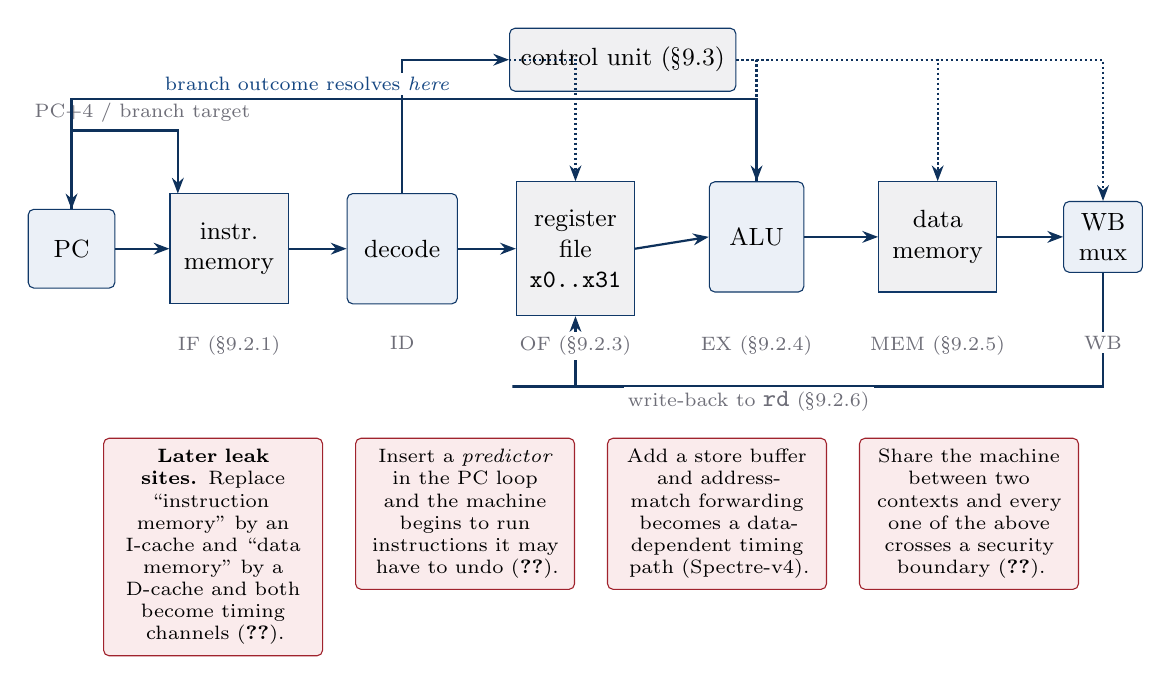
\begin{tikzpicture}[scale=1.0, every node/.style={font=\scriptsize}]
  % ---- stage blocks ------------------------------------------------
  \node[blk, minimum width=1.1cm, minimum height=1.0cm] (pc)  at (0,0)     {PC};
  \node[memblk, minimum width=1.5cm, minimum height=1.4cm] (imem) at (2.0,0) {instr.\\memory};
  \node[blk, minimum width=1.4cm, minimum height=1.4cm] (dec) at (4.2,0)   {decode};
  \node[memblk, minimum width=1.5cm, minimum height=1.7cm] (rf) at (6.4,0)  {register\\file\\\code{x0..x31}};
  \node[blk, minimum width=1.2cm, minimum height=1.4cm] (alu) at (8.7,0.15) {ALU};
  \node[memblk, minimum width=1.5cm, minimum height=1.4cm] (dmem) at (11.0,0.15){data\\memory};
  \node[blk, minimum width=1.0cm, minimum height=0.9cm] (wb)  at (13.1,0.15) {WB\\mux};

  % ---- control unit -------------------------------------------------
  \node[blk, minimum width=2.4cm, minimum height=0.8cm, fill=greyfill] (ctrl) at (7.0,2.4)
       {control unit (\SecRef{9.3})};
  \draw[sig] (dec.north) |- (ctrl.west);
  \foreach \t in {alu, dmem, wb} {\draw[sig, densely dotted] (ctrl.east) -| (\t.north);}
  \draw[sig, densely dotted] (ctrl.west) -| (rf.north);

  % ---- datapath wires ------------------------------------------------
  \draw[sig] (pc)   -- (imem);
  \draw[sig] (imem) -- (dec);
  \draw[sig] (dec)  -- (rf);
  \draw[sig] (rf.east)  -- (alu.west);
  \draw[sig] (alu.east) -- (dmem.west);
  \draw[sig] (dmem.east) -- (wb.west);
  % write-back path
  \draw[sig] (wb.south) |- (5.6,-1.75) -| (rf.south);
  \node[note, anchor=north] at (8.6,-1.75) {write-back to \code{rd} (\SecRef{9.2.6})};
  % PC + 4 loop
  \draw[sig] (pc.north) |- (0.9,1.5) -| (1.35,0.7);
  \node[note, anchor=south] at (0.9,1.55) {PC$+4$ / branch target};
  % branch resolution feedback
  \draw[sig] (alu.north) |- (5.0,1.9) -| (0,0.5);
  \node[note, anchor=south, text=accent] at (3.0,1.95) {branch outcome resolves \emph{here}};

  % ---- stage labels --------------------------------------------------
  \foreach \x/\l in {2.0/{IF (\SecRef{9.2.1})}, 4.2/{ID}, 6.4/{OF (\SecRef{9.2.3})},
                     8.7/{EX (\SecRef{9.2.4})}, 11.0/{MEM (\SecRef{9.2.5})}, 13.1/{WB}}
     {\node[note, anchor=north] at (\x,-1.05) {\l};}

  % ---- security annotations -------------------------------------------
  \node[atk, font=\scriptsize, text width=2.5cm, anchor=north west] at (0.4,-2.4)
       {\textbf{Later leak sites.} Replace ``instruction memory'' by an I-cache and
        ``data memory'' by a D-cache and both become timing channels
        (\Cref{ch:memsys}).};
  \node[atk, font=\scriptsize, text width=2.5cm, anchor=north west] at (3.6,-2.4)
       {Insert a \emph{predictor} in the PC loop and the machine begins to run
        instructions it may have to undo (\Cref{ch:pipeline}).};
  \node[atk, font=\scriptsize, text width=2.5cm, anchor=north west] at (6.8,-2.4)
       {Add a store buffer and address-match forwarding becomes a data-dependent
        timing path (Spectre-v4).};
  \node[atk, font=\scriptsize, text width=2.5cm, anchor=north west] at (10.0,-2.4)
       {Share the machine between two contexts and every one of the above
        crosses a security boundary (\Cref{ch:multicore}).};
\end{tikzpicture}
\caption[Single-cycle RISC-V datapath]{The reference single-cycle RV64I datapath
(textbook \SecRef{9.2}), with the control path of \SecRef{9.3} shown dotted. As
drawn, this machine has essentially no \uarchadj{} side channels: memory is a flat
array with fixed latency, the branch outcome is known before the next fetch, and
nothing is shared. The four red boxes name the optimisations that later chapters
add, and the channel each one opens.}
\label{fig:datapath}
\end{figure}

\paragraph{Instruction fetch (\SecRef{9.2.1}).} The PC addresses instruction
memory; the fetched word is the instruction. In the reference machine the PC
update is $\text{PC} \leftarrow \text{PC}+4$ or a computed target, and the choice
is made \emph{after} the branch condition is known. This is the property that
pipelining destroys.

\paragraph{Decode and operand fetch (\SecRef{9.2.2}, \SecRef{9.2.3}).} Because
the register specifiers occupy fixed positions in every format
(\Cref{fig:encoding}), the register file can be read in parallel with decoding.
The immediate is extracted and sign-extended according to format.

\paragraph{Execute (\SecRef{9.2.4}).} The ALU computes an
arithmetic result, an effective address, or a branch condition. One functional
unit, one result per cycle, no reordering.

\paragraph{Memory access (\SecRef{9.2.5}).} Loads read and stores write the data
memory. In the reference machine this takes a fixed time. \emph{The entire
subject of \Cref{ch:memsys} is what happens when it does not.}

\paragraph{Register write-back (\SecRef{9.2.6}).} The result is written to
\code{rd}, or discarded if the instruction has no destination. After write-back
the architectural state is exactly what \Cref{eq:contract} requires.

\paragraph{The control path (\SecRef{9.3}).} The control unit decodes the opcode
and function fields into the multiplexer selects and enables that steer the
datapath. In the single-cycle machine it is a combinational function of the
current instruction: it has no memory of earlier instructions. A branch
predictor changes that. It supplies the next fetch address from a table of past
outcomes, so control decisions come to depend on history, and history is state
that persists.\index{control unit}

\section{Where state appears when the machine is made fast}

\Cref{tab:stagestate} walks the stages again and names, for each, the
structure that a high-performance implementation adds, the information it
retains, and the chapter that analyses it.

\begin{table}[t]
\centering
\caption[Pipeline stages and the state added by optimisation]{The six stages of
the reference machine, the \uarchadj{} structures a high-performance
implementation adds to each, and where in this paper the resulting channel is
analysed.}
\label{tab:stagestate}
\footnotesize
\begin{tabularx}{\linewidth}{@{}p{2.1cm}>{\raggedright\arraybackslash}p{3.8cm}X>{\raggedright\arraybackslash}p{1.9cm}@{}}

\toprule
\textbf{Stage} & \textbf{Structure added} & \textbf{Information retained} & \textbf{Analysed in} \\
\midrule
Fetch    & I-cache, BTB, RAS, direction predictor &
Which lines were fetched; which branches were taken; call/return targets &
\Cref{ch:pipeline,ch:memsys} \\
Decode   & Micro-op cache, decoded-instruction buffers &
Which instructions were decoded recently & \Cref{ch:pipeline} \\
Operand fetch & Physical register file, rename map, issue queue &
Occupancy and readiness, hence dependence structure & \Cref{ch:pipeline} \\
Execute  & Multiple functional units, bypass network, execution window &
Port contention; which units were busy & \Cref{ch:pipeline,ch:transient} \\
Memory   & D-cache, TLB, page-walk cache, store buffer, LSQ, MSHRs &
Which lines and pages were touched; address matches for forwarding &
\Cref{ch:memsys} \\
Write-back & Reorder buffer, commit logic &
Retirement order and squash events (timing only) & \Cref{ch:pipeline,ch:transient} \\
\bottomrule
\end{tabularx}
\end{table}

\section{From the textbook datapath to open RISC-V cores}
\label{sec:opencores}

The open cores named in \Cref{sec:whyriscv} sit at three points between
\Cref{fig:datapath} and a modern out-of-order design, which is why they recur
as examples.

\begin{itemize}
  \item \textbf{Rocket}~\citep{asanovic2016rocket} pipelines the datapath into\index{Rocket core}
        five stages and adds caches, a TLB and a branch predictor. It executes
        in order, so a mispredicted branch is discovered within a few cycles.
  \item \textbf{CVA6}~\citep{zaruba2019ariane} is a six-stage, single-issue
        core that boots Linux. It is the platform on which the temporal fence
        of \Cref{ch:defenses} was built and measured.
  \item \textbf{BOOM}~\citep{celio2015berkeley,zhao2020sonicboom} is a\index{BOOM (SonicBOOM) core}
        superscalar out-of-order core with register renaming, a reorder buffer
        and a history-based predictor. It is the open core on which Spectre
        attacks were first replicated.
\end{itemize}

The simulator written for \Cref{ch:study} has the same two-layer structure as
this chapter and the next. Its functional core executes RV64IM instructions
exactly as the reference machine does, one at a time, and is checked against
QEMU; its timing layer then adds the pipeline, the predictors and the caches as
rules for \emph{when} each instruction is fetched, issued and committed
(\Cref{app:model}).

\begin{takeaway}
The reference machine has no \uarchadj{} channels and is far too slow to use.
Every structure that makes it fast remembers something about what ran before.
The design question on which this paper ends is therefore not whether the
channels can be removed, since returning to \Cref{fig:datapath} removes them,
but how much performance must be given back to close a particular one.
\end{takeaway}


\chapter{Pipelining, Speculation and the Birth of Transient State}
\label{ch:pipeline}

\begin{tocmapbox}
Background: textbook \SecRef{10.1}--\SecRef{10.3} (the pipelined processor and
its stages), \SecRef{10.4} (pipeline hazards), \SecRef{10.8} (support for
interrupts and exceptions) with \SecRef{10.8.2} (exceptions) and \SecRef{10.8.3}
(precise exceptions), \SecRef{10.9.3} (performance of a non-ideal pipeline),
\SecRef{10.10} (power and temperature issues), and \SecRef{10.11} (advanced
techniques) with \SecRef{10.11.1} (branch prediction) and \SecRef{10.11.4}
(out-of-order pipelines)~\citep{sarangi2025basic}.
\end{tocmapbox}

This chapter introduces the two properties that turn a passive timing
difference into something that can be steered: \emph{speculation}, by which the
machine executes instructions before it knows they are needed, and
\emph{squashing}, by which it erases their architectural effects.

\section{The pipeline and its hazards}

\Cref{fig:pipeline} shows the five-stage pipeline of textbook \SecRef{10.2},
which is essentially the organisation of Rocket~\citep{asanovic2016rocket}.\index{pipeline!five-stage}
Pipeline registers hold the state of the instructions in flight, up to five at
once. \Cref{tab:hazards} summarises the three hazard classes of \SecRef{10.4}
together with what the standard resolution of each leaves behind.

\begin{figure}[t]
\centering
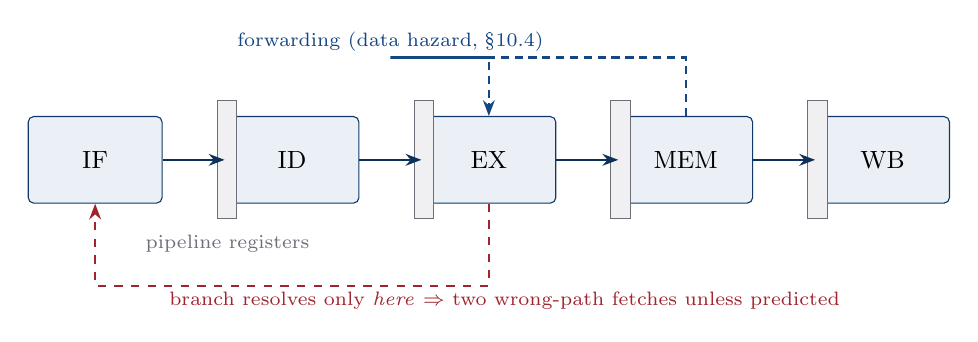
\begin{tikzpicture}[scale=1.0, every node/.style={font=\scriptsize}]
  \foreach \i/\x/\n in {0/0/IF, 1/2.5/ID, 2/5.0/EX, 3/7.5/MEM, 4/10.0/WB}
    {\node[blk, minimum width=1.7cm, minimum height=1.1cm] (s\i) at (\x,0) {\n};}
  \foreach \i/\x in {0/1.55, 1/4.05, 2/6.55, 3/9.05}
    {\draw[fill=greyfill, draw=muted] (\x,-0.75) rectangle ++(0.25,1.5);}
  \foreach \i [evaluate=\i as \j using int(\i+1)] in {0,1,2,3}
    {\draw[sig] (s\i.east) -- (s\j.west);}
  \node[note, anchor=north] at (1.68,-0.9) {pipeline registers};

  % hazards
  \draw[sig, densely dashed, draw=accent] (s3.north) |- (3.75,1.3) -| (s2.north);
  \node[note, anchor=south, text=accent] at (3.75,1.32) {forwarding (data hazard, \SecRef{10.4})};
  \draw[atksig] (s2.south) |- (2.5,-1.6) -| (s0.south);
  \node[note, anchor=north, text=attack] at (5.2,-1.62)
       {branch resolves only \emph{here} $\Rightarrow$ two wrong-path fetches unless predicted};
\end{tikzpicture}
\caption[Five-stage pipeline]{The five-stage pipeline of textbook
\SecRef{10.2}--\SecRef{10.3}. Forwarding paths resolve data hazards; the branch
outcome, however, is not known until EX, so the fetch stage must either stall or
\emph{guess}. Guessing is the origin of everything in \Cref{ch:transient}.}
\label{fig:pipeline}
\end{figure}

\begin{table}[t]
\centering
\caption[Hazards and their security consequence]{The three hazard classes
(\SecRef{10.4}), their standard resolution, and the security-relevant residue
each resolution leaves behind.}
\label{tab:hazards}
\footnotesize
\begin{tabularx}{\linewidth}{@{}p{2.2cm}p{4.2cm}X@{}}
\toprule
\textbf{Hazard} & \textbf{Standard resolution} & \textbf{Security-relevant residue} \\
\midrule
Data (RAW) & Forwarding; interlock and stall when a load feeds the next instruction &
Stall cycles are visible in timing; store-to-load forwarding is an
address-comparison whose outcome is data-dependent (Spectre-v4). \\
Control & Predict the branch; squash wrong-path instructions when the prediction
is resolved &
Wrong-path instructions \emph{execute} before being squashed. Their \uarchadj{}
effects are not undone. Spectre is built on that. \\
Structural & Duplicate the resource, or arbitrate &
Arbitration makes one context's timing depend on another's resource use, the mechanism of SMT and port-contention channels. \\
\bottomrule
\end{tabularx}
\end{table}

\section{Branch prediction}
\label{sec:bp}

To avoid stalling on every control hazard, the fetch stage predicts.\index{branch prediction}
\Cref{fig:predictors} sketches the usual hierarchy: a direction predictor built
from two-bit counters~\citep{smith1981study} and indexed by a hash of the
program counter and the global history~\citep{mcfarling1993combining}, a branch
target buffer, and a return-address stack. SonicBOOM uses a tagged
geometric-history predictor~\citep{seznec2006case,zhao2020sonicboom}, a more
accurate member of the same family. \Cref{app:predictors} works through each
structure.

\begin{figure}[t]
\centering
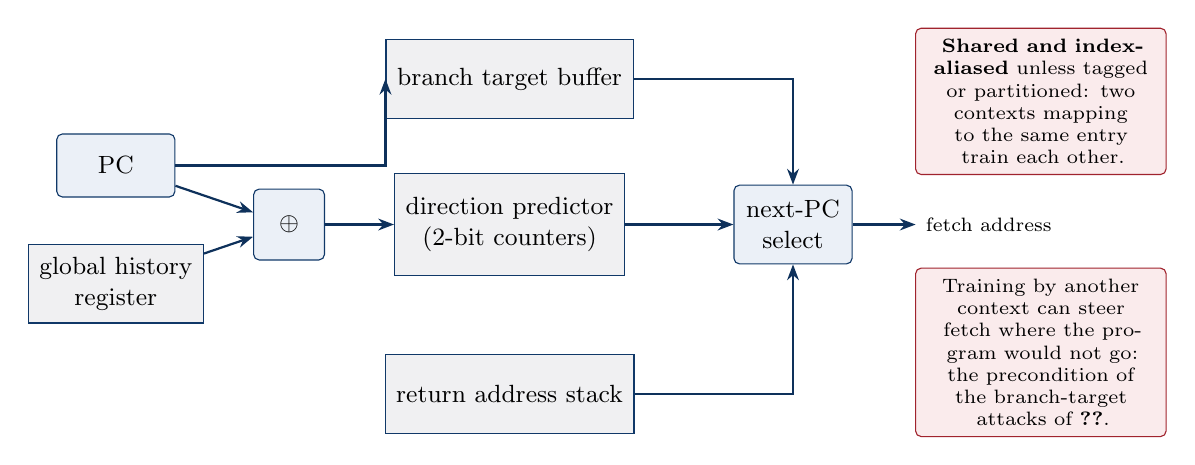
\begin{tikzpicture}[scale=1.0, every node/.style={font=\scriptsize}]
  \node[blk, minimum width=1.5cm] (pc) at (0,0) {PC};
  \node[memblk, minimum width=1.9cm, minimum height=1.0cm] (ghr) at (0,-1.5) {global history\\register};
  \node[blk, minimum width=0.9cm, minimum height=0.9cm] (xor) at (2.2,-0.75) {$\oplus$};
  \node[memblk, minimum width=2.3cm, minimum height=1.3cm] (bht) at (5.0,-0.75)
       {direction predictor\\(2-bit counters)};
  \node[memblk, minimum width=2.3cm, minimum height=1.0cm] (btb) at (5.0,1.1) {branch target buffer};
  \node[memblk, minimum width=2.3cm, minimum height=1.0cm] (ras) at (5.0,-2.9) {return address stack};
  \node[blk, minimum width=1.5cm, minimum height=1.0cm] (nxt) at (8.6,-0.75) {next-PC\\select};

  \draw[sig] (pc) -- (xor); \draw[sig] (ghr) -- (xor);
  \draw[sig] (xor) -- (bht);
  \draw[sig] (pc.east) -| (btb.west);
  \draw[sig] (bht) -- (nxt); \draw[sig] (btb.east) -| (nxt.north);
  \draw[sig] (ras.east) -| (nxt.south);
  \draw[sig] (nxt.east) -- ++(0.8,0) node[right] {fetch address};

  %% Anchored north/south so the two callouts grow away from each other; the
  %% atk style would otherwise override the picture-wide \scriptsize and collide.
  \node[atk, text width=2.9cm, font=\scriptsize, anchor=north west] at (10.15,1.75)
       {\textbf{Shared and index-aliased} unless tagged or partitioned: two contexts mapping to
        the same entry train each other.};
  \node[atk, text width=2.9cm, font=\scriptsize, anchor=south west] at (10.15,-3.45)
       {Training by another context can steer fetch where the program would not go:
        the precondition of the branch-target attacks of \Cref{ch:transient}.};

\end{tikzpicture}
\caption[Branch prediction structures]{Branch prediction structures
(\SecRef{10.11.1}). The direction predictor is indexed by a hash of the PC and
the global history, so unrelated branches can share an entry. The BTB and the
RAS supply targets. All three are \uarchadj{} state in the sense of
\Cref{sec:archvsuarch}; whether an entry written by one context is used by
another depends on how the implementation tags, partitions or flushes the
tables.}
\label{fig:predictors}
\end{figure}

\Cref{tab:predictor} shows what prediction is worth on the eleven kernels of the
model study, for the default predictor of the model (4096 two-bit counters
indexed gshare-fashion with twelve bits of history, a 512-entry BTB and a
16-entry RAS), for a bimodal predictor without history, and for a static
predict-not-taken policy. With gshare the kernels mispredict between
\R{bp.gshare.stream}\pc{} and \R{bp.gshare.bstree}\pc{} of their conditional
branches. With the static policy the kernels dominated by loops,
\code{matmul}, \code{sieve}, \code{stream} and \code{strsearch}, lose more
than half of their performance.

\begin{table}[t]
\centering
\caption[Branch prediction in the model study]{Misprediction rate of
conditional branches and instructions per cycle for three direction predictors
in the model of \Cref{ch:study}. The predictor is what makes a wide pipeline
worth building, and the kernels with data-dependent branches are the ones that
keep mispredicting.}
\label{tab:predictor}
\footnotesize
%% BEGIN GENERATED tab_predictor
\begin{tabular}{@{}l@{\hspace{12pt}}rr@{\hspace{12pt}}rr@{\hspace{12pt}}rr@{}}
\toprule
 & \multicolumn{2}{c}{\textbf{gshare}} & \multicolumn{2}{c}{\textbf{bimodal}} & \multicolumn{2}{c}{\textbf{static not-taken}} \\
\textbf{Kernel} & \textbf{mis.\,\%} & \textbf{IPC} & \textbf{mis.\,\%} & \textbf{IPC} & \textbf{mis.\,\%} & \textbf{IPC} \\
\midrule
\texttt{matmul} & 1.6 & 3.70 & 1.5 & 3.71 & 98.5 & 0.91 \\
\texttt{heapsort} & 15.3 & 1.48 & 14.4 & 1.50 & 19.5 & 1.39 \\
\texttt{listwalk} & 0.1 & 0.19 & 0.0 & 0.19 & 88.9 & 0.16 \\
\texttt{bsearch} & 16.7 & 0.56 & 16.5 & 0.56 & 26.3 & 0.51 \\
\texttt{bstree} & 17.4 & 0.43 & 18.9 & 0.41 & 45.8 & 0.30 \\
\texttt{crc32} & 0.7 & 1.23 & 0.4 & 1.24 & 99.6 & 1.05 \\
\texttt{sieve} & 2.4 & 2.54 & 2.3 & 2.57 & 97.7 & 0.37 \\
\texttt{hashtab} & 17.3 & 0.79 & 20.3 & 0.81 & 32.3 & 0.62 \\
\texttt{stream} & 0.0 & 2.22 & 0.0 & 2.22 & 100.0 & 1.07 \\
\texttt{fibcall} & 4.7 & 2.42 & 50.0 & 1.36 & 50.0 & 1.38 \\
\texttt{strsearch} & 10.9 & 1.56 & 10.6 & 1.58 & 90.9 & 0.59 \\
\bottomrule
\end{tabular}
%% END GENERATED tab_predictor
\end{table}

The security cost of prediction is structural. A predictor is a memory that\index{predictor!aliasing between domains}
every context writes and reads, and unless the implementation prevents it, one
context's training influences another's predictions. Evtyushkin \etal{} showed
that the direction predictor alone is a usable
channel~\citep{evtyushkin2018branchscope}, and branch-history injection showed
that isolating the target tables is not enough if the history that indexes them\index{Spectre!v2, branch target injection}
is shared~\citep{barberis2022bhi}.

\section{Precise exceptions and what a squash restores}
\label{sec:precise}

Textbook \SecRef{10.8.3} defines a \emph{precise} exception: all instructions\index{precise exceptions}
before the faulting one have completed, none after it has had any effect, and
the architectural state is as if the program had stopped at that instruction.
RISC-V requires precise traps~\citep{riscv-priv}. The same recovery mechanism
is used for a mispredicted branch: the instructions fetched after it are
discarded, and architecturally they never happened.

The definition quantifies over architectural state, because when the mechanism
was standardised~\citep{smith1988precise} that was the state that mattered for
correctness. \Cref{fig:squash} makes the consequence concrete on the five-stage
machine.

\begin{figure}[t]
\centering
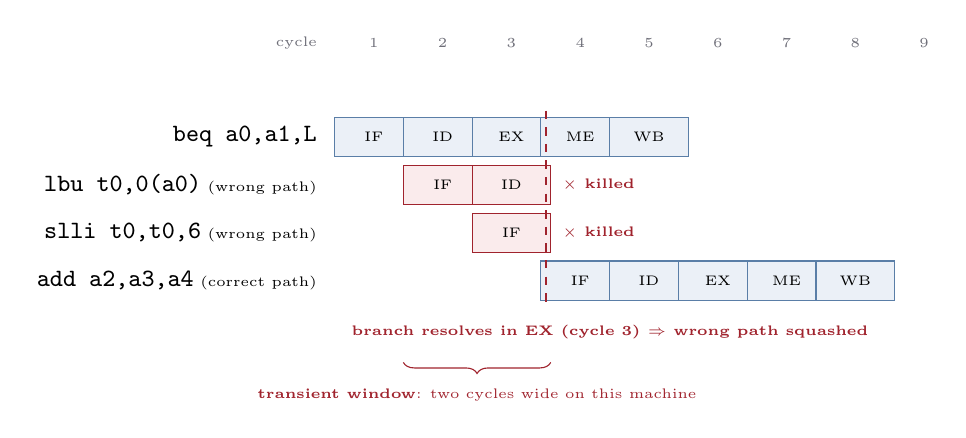
\begin{tikzpicture}[scale=0.78, every node/.style={font=\scriptsize}]
  % column headers
  \foreach \c in {1,...,9} {\node[text=muted, font=\tiny] at (\c*1.12, 0.75) {\c};}
  \node[anchor=east, text=muted, font=\tiny] at (0.35,0.75) {cycle};
  % rows: row / label / first cycle / stages actually completed / 1 = wrong path
  \foreach \r/\name/\start/\nst/\bad in {%
      1/{\code{beq a0,a1,L}}/1/5/0,
      2/{\code{lbu t0,0(a0)} (wrong path)}/2/2/1,
      3/{\code{slli t0,t0,6} (wrong path)}/3/1/1,
      4/{\code{add a2,a3,a4} (correct path)}/4/5/0}
  {
    \node[anchor=east, font=\tiny] at (0.35,-\r*0.78) {\name};
    \foreach \s [count=\i from 0] in {IF,ID,EX,ME,WB}
    {
      \ifnum\i<\nst\relax
        \pgfmathsetmacro{\cx}{(\start+\i)*1.12}
        \ifnum\bad=1\relax
          \node[draw=attack, fill=attackfill, minimum width=1.0cm, minimum height=0.5cm,
                inner sep=0pt, font=\tiny] at (\cx,-\r*0.78) {\s};
        \else
          \node[draw=accent!70, fill=lightfill, minimum width=1.0cm, minimum height=0.5cm,
                inner sep=0pt, font=\tiny] at (\cx,-\r*0.78) {\s};
        \fi
      \fi
    }
    % "killed here" marker for the wrong-path rows
    \ifnum\bad=1\relax
      \pgfmathsetmacro{\kx}{(\start+\nst)*1.12}
      \node[text=attack, font=\tiny\bfseries, anchor=west] at (\kx-0.45,-\r*0.78)
            {$\times$ killed};
    \fi
  }
  % squash marker: end of cycle 3
  \draw[attack, thick, dashed] (3.92,-0.35) -- (3.92,-3.55);
  \node[anchor=west, text=attack, font=\tiny\bfseries] at (0.6,-3.95)
       {branch resolves in EX (cycle~3) $\Rightarrow$ wrong path squashed};
  % transient window brace: the two wrong-path fetches, cycles 2--3
  \draw[decorate, decoration={brace, amplitude=4pt, mirror}, attack]
       (1.6,-4.45) -- (4.0,-4.45)
       node[midway, below=6pt, text=attack, align=center, font=\tiny]
       {\textbf{transient window}: two cycles wide on this machine};
\end{tikzpicture}
\caption[Squashed instructions leave state behind]{Pipeline diagram of a
mispredicted branch on the five-stage machine of \Cref{fig:pipeline}. The branch
resolves in EX at the end of cycle~3, so the two wrong-path instructions (red)
are killed in ID and in IF and never reach the memory stage. Precise exception
semantics (\SecRef{10.8.3}) guarantee that their \emph{architectural} effects
vanish; what does \emph{not} vanish is the instruction-cache line fetched for the
wrong path and the predictor entry that sent the machine there. Driving the
\emph{data} cache transiently, which is the transmitter of \Cref{ch:transient},
needs a window far wider than two cycles, and \Cref{sec:ooo} shows where that
window comes from.}
\label{fig:squash}
\end{figure}

\begin{takeaway}
A squash is architecturally complete. What it does to \uarchadj{} state is a
design decision, and conventional cores leave that state as the wrong path left
it. A core that restored cache, TLB and predictor state at every squash would
remove the persistent trace; it would not remove the contention that transient
instructions cause while they are still running (\Cref{sec:attacksdef}), and it
would add work to every misprediction. Most defences of \Cref{ch:defenses} are
ways of making one of the two, the undo or the concealment, cheap.
\end{takeaway}

\section{Out-of-order execution and the size of the window}
\label{sec:ooo}

Textbook \SecRef{10.11.4} introduces out-of-order execution: instructions are\index{out-of-order execution}
renamed, dispatched into issue queues, executed as soon as their operands are
ready~\citep{tomasulo1967efficient}, and retired in program order from a
reorder buffer.\index{reorder buffer (ROB)} \Cref{fig:ooo} sketches the organisation.

\begin{figure}[t]
\centering
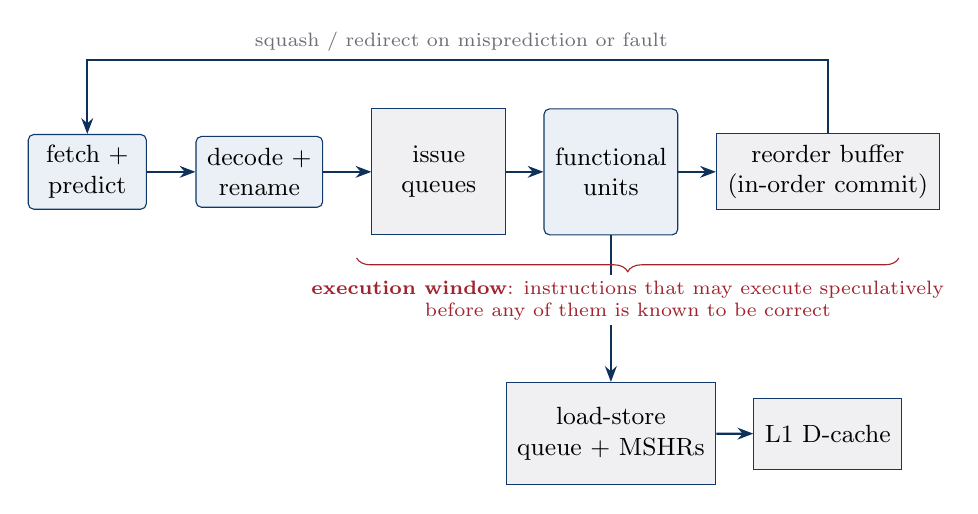
\begin{tikzpicture}[scale=0.95, every node/.style={font=\scriptsize}]
  \node[blk, minimum width=1.5cm, minimum height=0.9cm] (fe) at (0,0) {fetch +\\predict};
  \node[blk, minimum width=1.5cm, minimum height=0.9cm] (rn) at (2.3,0) {decode +\\rename};
  \node[memblk, minimum width=1.7cm, minimum height=1.6cm] (iq) at (4.7,0) {issue\\queues};
  \node[blk, minimum width=1.5cm, minimum height=1.6cm] (fu) at (7.0,0) {functional\\units};
  \node[memblk, minimum width=1.7cm, minimum height=1.3cm] (lsq) at (7.0,-3.5) {load-store\\queue + MSHRs};
  \node[memblk, minimum width=1.9cm, minimum height=0.9cm] (rob) at (9.9,0) {reorder buffer\\(in-order commit)};
  \node[memblk, minimum width=1.7cm, minimum height=0.9cm] (dc) at (9.9,-3.5) {L1 D-cache};

  \draw[sig] (fe)--(rn); \draw[sig] (rn)--(iq); \draw[sig] (iq)--(fu);
  \draw[sig] (fu)--(rob);
  \draw[sig] (fu.south)--(lsq.north);
  \draw[sig] (lsq)--(dc);
  \draw[sig] (rob.north) |- (5.0,1.5) -| (fe.north);
  \node[note, anchor=south] at (5.0,1.55) {squash / redirect on misprediction or fault};

  \draw[decorate, decoration={brace, amplitude=5pt, mirror}, attack]
       (3.6,-1.15) -- (10.85,-1.15)
       node[midway, below=6pt, text=attack, align=center, font=\scriptsize,
            fill=white, inner sep=2pt]
       {\textbf{execution window}: instructions that may execute speculatively\\
        before any of them is known to be correct};
\end{tikzpicture}
\caption[Out-of-order organisation]{Out-of-order organisation
(\SecRef{10.11.4}). The reorder buffer restores in-order, precise architectural
semantics on top of out-of-order execution. The reorder buffer, the issue
queues and the load queue bound how many instructions can be in flight;
operand readiness and the time at which a prediction resolves decide which of
them execute before a squash.}
\label{fig:ooo}
\end{figure}

How many instructions execute on a wrong path is decided by two quantities, not\index{speculation window}
one. The reorder buffer bounds how many can be \emph{in flight}; the time the
mispredicted branch takes to resolve bounds how many of those are fetched and
issued before the squash. A branch whose operands are ready resolves a cycle
after it is dispatched and leaves almost no window, whatever the size of the
buffer. A branch that waits for a load that misses the cache leaves a window of
tens or hundreds of cycles. \Cref{app:pipeline} derives the relation
\begin{equation}
  N_{\text{transient}} \;\le\; \min\bigl(R,\; W \cdot (t_{\text{resolve}} - t_{\text{dispatch}})\bigr),
  \label{eq:window}
\end{equation}
for a core of width $W$ with $R$ reorder-buffer entries.\index{in-order versus out-of-order cores}

\section{How large the window is: results from the model}
\label{sec:windowresults}

The model of \Cref{ch:study} executes the wrong path explicitly after each
misprediction, so the transient work can be counted. \Cref{fig:window} shows
the count per squash against the size of the reorder buffer, and
\Cref{tab:window} gives the detail for the default of 128 entries.

\begin{figure}[t]
\centering
%% BEGIN GENERATED fig_window
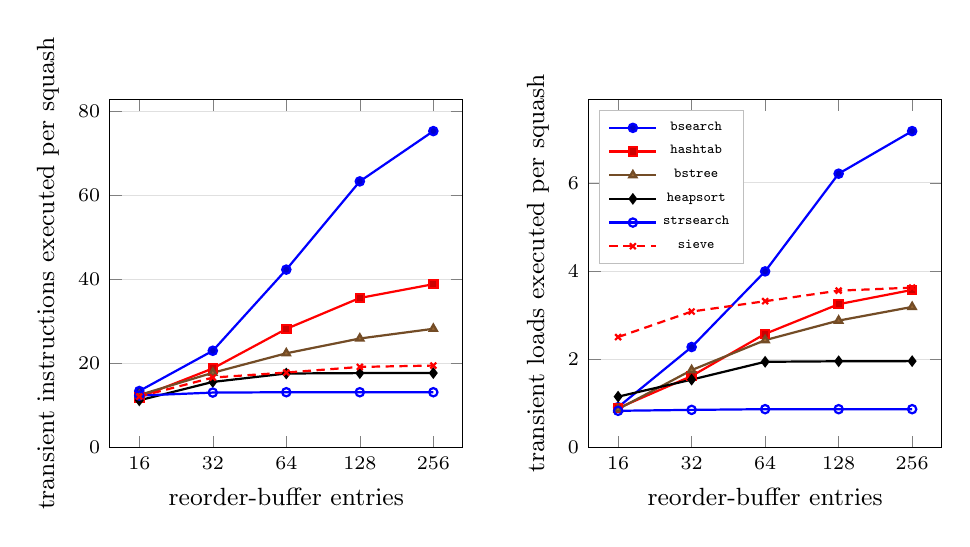
\begin{tikzpicture}
\begin{groupplot}[group style={group size=2 by 1, horizontal sep=1.6cm},
  width=0.50\linewidth, height=6.0cm, xmode=log, log basis x=2,
  xtick={16,32,64,128,256}, xticklabels={16,32,64,128,256},
  xlabel={reorder-buffer entries}, tick label style={font=\scriptsize},
  label style={font=\small}, ymajorgrids, grid style={draw=black!12},
  legend style={font=\tiny, draw=black!25}, ymin=0]
\nextgroupplot[ylabel={transient instructions executed per squash}]
\addplot+[mark=*, mark size=1.5pt, thick] coordinates {(16,13.417) (32,22.994) (64,42.301) (128,63.292) (256,75.256)};
\addplot+[mark=square*, mark size=1.5pt, thick] coordinates {(16,11.912) (32,18.784) (64,28.192) (128,35.551) (256,38.830)};
\addplot+[mark=triangle*, mark size=1.5pt, thick] coordinates {(16,12.461) (32,17.759) (64,22.391) (128,25.909) (256,28.219)};
\addplot+[mark=diamond*, mark size=1.5pt, thick] coordinates {(16,11.194) (32,15.576) (64,17.583) (128,17.676) (256,17.693)};
\addplot+[mark=o, mark size=1.5pt, thick] coordinates {(16,12.329) (32,13.042) (64,13.126) (128,13.126) (256,13.126)};
\addplot+[mark=x, mark size=1.5pt, thick] coordinates {(16,12.091) (32,16.614) (64,17.811) (128,19.149) (256,19.470)};
\nextgroupplot[ylabel={transient loads executed per squash}, legend pos=north west]
\addplot+[mark=*, mark size=1.5pt, thick] coordinates {(16,0.913) (32,2.277) (64,3.993) (128,6.210) (256,7.176)};
\addlegendentry{\texttt{bsearch}}
\addplot+[mark=square*, mark size=1.5pt, thick] coordinates {(16,0.890) (32,1.619) (64,2.576) (128,3.249) (256,3.573)};
\addlegendentry{\texttt{hashtab}}
\addplot+[mark=triangle*, mark size=1.5pt, thick] coordinates {(16,0.868) (32,1.753) (64,2.433) (128,2.877) (256,3.187)};
\addlegendentry{\texttt{bstree}}
\addplot+[mark=diamond*, mark size=1.5pt, thick] coordinates {(16,1.151) (32,1.537) (64,1.942) (128,1.954) (256,1.957)};
\addlegendentry{\texttt{heapsort}}
\addplot+[mark=o, mark size=1.5pt, thick] coordinates {(16,0.830) (32,0.851) (64,0.867) (128,0.867) (256,0.867)};
\addlegendentry{\texttt{strsearch}}
\addplot+[mark=x, mark size=1.5pt, thick] coordinates {(16,2.503) (32,3.082) (64,3.317) (128,3.556) (256,3.625)};
\addlegendentry{\texttt{sieve}}
\end{groupplot}
\end{tikzpicture}
%% END GENERATED fig_window
\caption[Transient work per squash against reorder-buffer size]{Transient
instructions (left) and transient loads (right) executed per squash in the
model, against the number of reorder-buffer entries. The curves saturate where
the resolution time of the branch, not the buffer, becomes the limit, as
\Cref{eq:window} predicts.}
\label{fig:window}
\end{figure}

\begin{table}[t]
\centering
\caption[Transient execution per kernel]{Transient execution in the model with a
128-entry reorder buffer and no defence. \emph{Disp.}, \emph{Exec.} and
\emph{Loads} are wrong-path instructions dispatched, executed and loads
executed, per squash. \emph{Fills} counts first-level cache fills caused by
transient loads over the whole run. \emph{Dep.\ loads} are transient loads
whose address was computed from the value of another transient load, and
\emph{Dep.\ fills} the fills they caused.}
\label{tab:window}
\footnotesize
%% BEGIN GENERATED tab_window
\begin{tabular}{@{}lrrrrrrr@{}}
\toprule
\textbf{Kernel} & \textbf{Squashes} & \textbf{Disp.} & \textbf{Exec.} & \textbf{Loads} & \textbf{Fills} & \textbf{Dep.\ loads} & \textbf{Dep.\ fills} \\
\midrule
\texttt{matmul} & 4\,300 & 8.0 & 2.0 & 1.91 & 56 & 0 & 0 \\
\texttt{heapsort} & 63\,106 & 29.7 & 17.7 & 1.95 & 13\,753 & 0 & 0 \\
\texttt{listwalk} & 80 & 10.8 & 4.0 & 0.89 & 4 & 32 & 2 \\
\texttt{bsearch} & 140\,010 & 82.0 & 63.3 & 6.21 & 422\,092 & 0 & 0 \\
\texttt{bstree} & 358\,660 & 32.0 & 25.9 & 2.88 & 131 & 7\,189 & 131 \\
\texttt{crc32} & 2\,033 & 9.3 & 3.3 & 0.00 & 1 & 0 & 0 \\
\texttt{sieve} & 19\,313 & 28.1 & 19.1 & 3.56 & 1\,109 & 0 & 0 \\
\texttt{hashtab} & 118\,064 & 51.5 & 35.6 & 3.25 & 90\,287 & 0 & 0 \\
\texttt{stream} & 68 & 6.0 & 2.4 & 0.12 & 8 & 0 & 0 \\
\texttt{fibcall} & 11\,466 & 9.9 & 5.0 & 0.00 & 0 & 0 & 0 \\
\texttt{strsearch} & 48\,096 & 16.2 & 13.1 & 0.87 & 267 & 0 & 0 \\
\bottomrule
\end{tabular}
%% END GENERATED tab_window
\end{table}

\begin{finding}
In \code{bsearch}, where each branch waits for a load from a large table, a
squash discards \R{wp.exec.bsearch} executed instructions on average with 128
reorder-buffer entries, against \R{wp.exec16.bsearch} with 16 and
\R{wp.exec256.bsearch} with 256. Over the run the transient loads of this one
kernel install \R{wp.fills.bsearch} lines in the first-level cache that no
committed instruction had asked for at the time. In \code{bstree}, \R{wp.dep.bstree}
transient loads used an address that had itself been loaded transiently: the
access-then-transmit shape of \Cref{ch:transient} occurs in an ordinary tree
search, without any attacker.
\end{finding}

Two observations follow. The window grows with the same parameters that buy
performance: a larger buffer and a wider pipeline both raise the number of
instructions that run before a squash. And wrong-path memory references are not
rare events: they are a constant by-product of speculation, known in the
performance literature for their prefetching and polluting
effects~\citep{mutlu2005analysis} long before they were a security concern.

\section{Metrics: what a defence costs}
\label{sec:metrics}

Pricing a defence needs four quantities: execution time through the iron law,
relative slowdown against an undefended baseline, dynamic power, and the
energy-delay product. Their definitions and the conditions under which each is
a valid comparison are set out in \Cref{app:metrics}. One point belongs here,
next to the machinery that creates the cost: a slowdown quoted as a ratio of
IPCs equals a ratio of execution times only if the defence changes neither the
dynamic instruction count nor the clock period, and software defences change
the first while hardware defences can change the second.


\chapter{The Memory System as an Attack Surface}
\label{ch:memsys}

\begin{tocmapbox}
Background: textbook \SecRef{11.1.2}--\SecRef{11.1.8} (memory access patterns,
temporal and spatial locality, hierarchical memory, cache blocks), \SecRef{11.2}
(caches), \SecRef{11.3} (the memory system) with \SecRef{11.3.1} (its
mathematical model), and \SecRef{11.4} (virtual memory) with \SecRef{11.4.2}
(the overlap and size problems), \SecRef{11.4.3} (implementation of virtual
memory with paging) and \SecRef{11.4.5} (the memory management
unit)~\citep{sarangi2025basic}.
\end{tocmapbox}

\Cref{ch:memories} explained why an array access takes time and
\Cref{ch:pipeline} why a processor runs instructions it may have to undo. This
chapter turns to the memory hierarchy: where loads are served, what that costs,
and how the difference is measured.

\section{Locality, hierarchy, and where loads are served}

Caches exist because programs exhibit temporal and spatial locality\index{locality!temporal and spatial}
(\SecRef{11.1.2}--\SecRef{11.1.5}). The hierarchy exploits it by placing a small
fast array close to the pipeline and larger, slower arrays behind it.
\Cref{fig:hierarchy} shows the four service latencies used in the model of this
paper, and \Cref{fig:service} shows how the loads of each kernel divide among
the levels.

\begin{figure}[t]
\centering
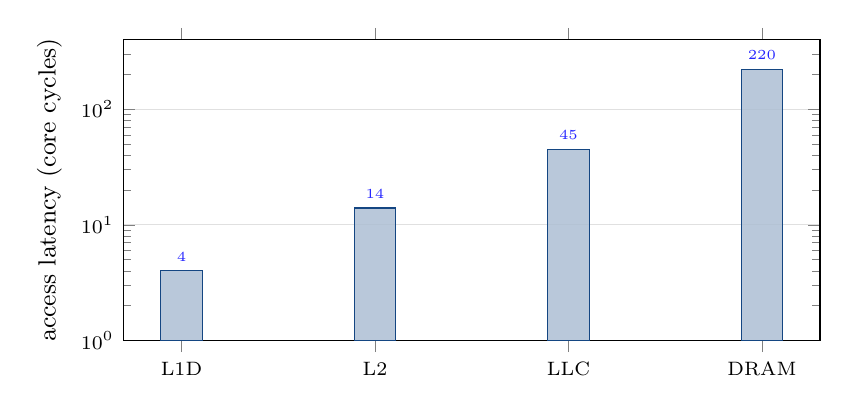
\begin{tikzpicture}
\begin{axis}[
  barstyle, height=5.4cm, width=0.86\linewidth,
  ybar, bar width=15pt,
  symbolic x coords={L1D,L2,LLC,DRAM},
  xtick=data, ymode=log, log basis y=10,
  ymin=1, ymax=400,
  ylabel={access latency (core cycles)},
  %% On a log axis pgfplots' default point meta is log10(y), so the bar labels
  %% must be given explicitly, otherwise they print 0.6, 1.15, ... not 4, 14, ...
  point meta=explicit symbolic,
  nodes near coords, nodes near coords style={font=\tiny},
  ]
  \addplot+[fill=accent!35, draw=accent] coordinates {
      (L1D,4) [4] (L2,14) [14] (LLC,45) [45] (DRAM,220) [220]};
\end{axis}
\end{tikzpicture}
\caption[Latencies of the memory hierarchy in the model]{The four load
latencies of the model of \Cref{ch:study}, on a logarithmic scale: a load
served by the first-level cache, by the second level, by the last-level cache
and by memory. These are \emph{parameters} of the model, chosen to be typical of
an application-class core; they are inputs, not measurements. What matters for
this chapter is the ratio: the fastest and the slowest service differ by a
factor of 55.}
\label{fig:hierarchy}
\end{figure}

\begin{figure}[t]
\centering
%% BEGIN GENERATED fig_service
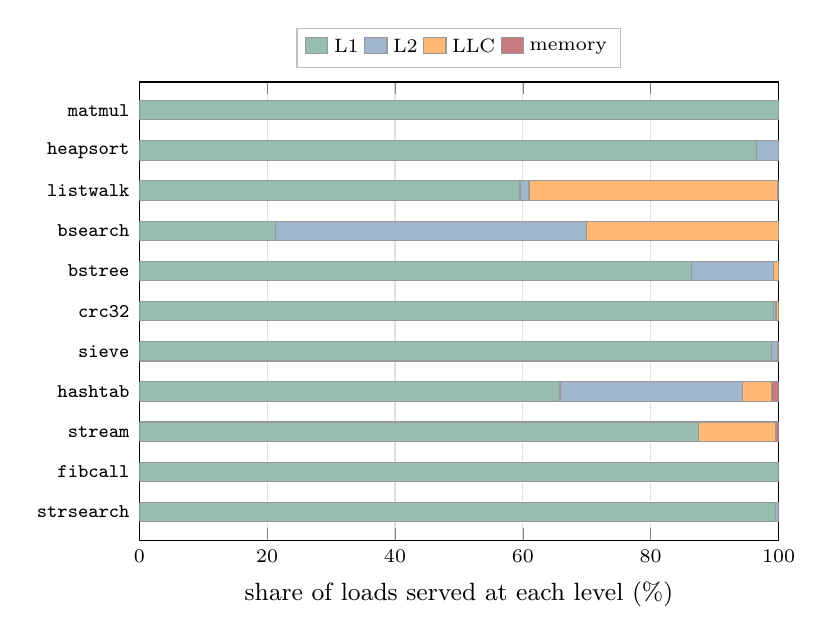
\begin{tikzpicture}
\begin{axis}[xbar stacked, width=0.80\linewidth, height=7.4cm,
  bar width=7pt, xmin=0, xmax=100, enlarge y limits=0.07,
  symbolic y coords={strsearch,fibcall,stream,hashtab,sieve,crc32,bstree,bsearch,listwalk,heapsort,matmul}, ytick=data,
  yticklabel style={font=\scriptsize\ttfamily}, xticklabel style={font=\scriptsize},
  xlabel={share of loads served at each level (\%)}, label style={font=\small},
  legend style={font=\scriptsize, draw=black!25, at={(0.5,1.03)}, anchor=south,
    legend columns=4}, xmajorgrids, grid style={draw=black!12}]
\addplot+[fill=defense!45, draw=black!40] coordinates {(99.497,strsearch) (100.000,fibcall) (87.501,stream) (65.808,hashtab) (98.963,sieve) (99.216,crc32) (86.386,bstree) (21.344,bsearch) (59.558,listwalk) (96.522,heapsort) (99.925,matmul)};
\addlegendentry{L1}
\addplot+[fill=accent!40, draw=black!40] coordinates {(0.503,strsearch) (0.000,fibcall) (0.019,stream) (28.509,hashtab) (0.844,sieve) (0.377,crc32) (12.839,bstree) (48.573,bsearch) (1.406,listwalk) (3.466,heapsort) (0.075,matmul)};
\addlegendentry{L2}
\addplot+[fill=orange!55, draw=black!40] coordinates {(0.000,strsearch) (0.000,fibcall) (11.998,stream) (4.616,hashtab) (0.193,sieve) (0.407,crc32) (0.775,bstree) (30.083,bsearch) (38.933,listwalk) (0.012,heapsort) (0.000,matmul)};
\addlegendentry{LLC}
\addplot+[fill=attack!60, draw=black!40] coordinates {(0.000,strsearch) (0.000,fibcall) (0.483,stream) (1.067,hashtab) (0.000,sieve) (0.000,crc32) (0.000,bstree) (0.000,bsearch) (0.104,listwalk) (0.000,heapsort) (0.000,matmul)};
\addlegendentry{memory}
\end{axis}
\end{tikzpicture}
%% END GENERATED fig_service
\caption[Where the loads of each kernel are served]{Share of committed loads
served by each level of the hierarchy in the model (32\,KiB first level,
256\,KiB second level, 2\,MiB last level). The kernels were chosen to spread
across the hierarchy: \code{fibcall} and \code{matmul} live in the first level,
while \code{bsearch} and \code{listwalk} take a large share of their loads from
the last.}
\label{fig:service}
\end{figure}

What an observer times is not the array of \Cref{fig:readtiming} but the whole
service path of a load. \Cref{fig:hitmiss} draws that view: one load, issued in
one cycle, returns its data at two different times depending on where the line
is found.

\begin{figure}[t]
\centering
\small
\begin{tikztimingtable}[timing/slope=0.08, xscale=1.9, yscale=1.5,
                        timing/rowdist=3.2ex,
                        timing/name/.style={font=\scriptsize}]
  \texttt{clk}                          & 14{C} \\
  load issued (\code{lbu t2,0(t1)})     & L H 12L \\
  data returned, L1 \emph{hit}       & 4L H 9L \\
  data returned, L1 \emph{miss}      & 11L H 2L \\
  attacker's timer                      & 2D{\texttt{rdcycle}} 9D{measured interval} 3D{\texttt{rdcycle}} \\
\end{tikztimingtable}
\par\vspace{2pt}
\caption[Hit versus miss on the load interface]{The measurement, drawn on the
core's load interface. One load instruction, one issue cycle, two return times.
The attacker brackets the load with two reads of the cycle counter and
classifies the interval against a threshold; the horizontal gap between rows
three and four is the entire channel. The miss latency is drawn compressed; the true gap is far wider, as \Cref{fig:hierarchy} shows.}
\label{fig:hitmiss}
\end{figure}

\section{Cache organisation and the address split}

Textbook \SecRef{11.2} develops the set-associative cache. An address is split
into three fields (\Cref{fig:addrsplit}): the block offset selects a byte\index{cache!address split}
within a line, the index selects a set, and the tag is compared with the tags
of all ways of that set. \Cref{app:caches} works through a lookup, the
replacement policies and a numerical example.

\begin{figure}[t]
\centering
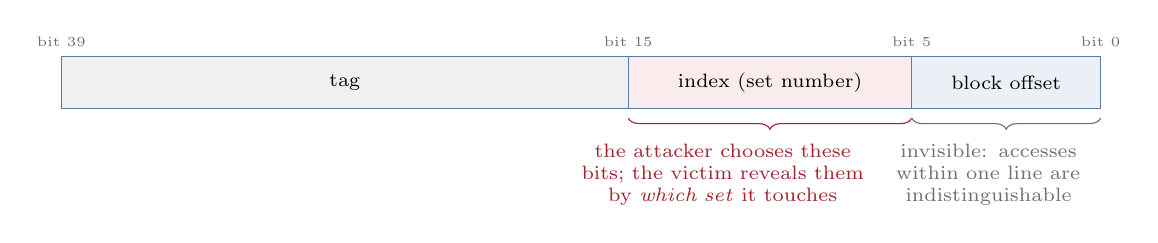
\begin{tikzpicture}[x=4.0mm, y=1cm]
  \newcommand{\afld}[5]{%
    \draw[fill=#5, draw=accent!70, line width=0.3pt] (#1,#2) rectangle ++(#3,0.66);
    \node[font=\scriptsize] at ({#1+#3/2}, {#2+0.33}) {#4};}
  \afld{0}{0}{18}{tag}{greyfill}
  \afld{18}{0}{9}{index (set number)}{attackfill}
  \afld{27}{0}{6}{block offset}{lightfill}
  \node[font=\tiny, text=muted] at (0,0.85) {bit 39};
  \node[font=\tiny, text=muted] at (18,0.85) {bit 15};
  \node[font=\tiny, text=muted] at (27,0.85) {bit 5};
  \node[font=\tiny, text=muted] at (33,0.85) {bit 0};
  % braces
  \draw[decorate, decoration={brace, amplitude=4pt, mirror}, attack] (18,-0.12) -- (27,-0.12);
  \draw[decorate, decoration={brace, amplitude=4pt, mirror}, muted]  (27,-0.12) -- (33,-0.12);
  % annotations, each kept inside its own horizontal band
  \node[font=\scriptsize, text=attack, align=center, text width=3.8cm,
        anchor=north] at (21,-0.32)
        {the attacker chooses these bits; the victim reveals them by
         \emph{which set} it touches};
  \node[font=\scriptsize, text=muted, align=center, text width=2.6cm,
        anchor=north east] at (33,-0.32)
        {invisible: accesses within one line are indistinguishable};
\end{tikzpicture}
\caption[Cache address split]{Address split for a \SI{256}{\kibi\byte},
8-way, \SI{64}{\byte}-line cache with a 40-bit physical address
(\SecRef{11.2}). The block offset determines the \emph{granularity of the
channel}: an attacker learns which \SI{64}{\byte} line was touched, never which
byte. Cryptographic implementations that fit a table into one line are therefore
immune to this particular channel, and table-free or scatter-gather AES
implementations were the first software mitigation for that reason.}
\label{fig:addrsplit}
\end{figure}

Three design parameters determine what an observation of the cache resolves.

\begin{itemize}
  \item \textbf{Associativity} $W$. A line can be displaced from a set only by
        bringing $W$ other lines into it. Higher associativity also removes
        conflict misses~\citep{hill1989evaluating}, which is why it is chosen.
  \item \textbf{Replacement policy.} Under true LRU the line displaced is a
        deterministic function of the access order; tree-based approximations
        and random replacement make it less predictable.\index{Prime+Probe}
  \item \textbf{Inclusivity.} In an inclusive hierarchy a line evicted from the
        last level must leave the private caches too, so activity in the shared\index{cache!inclusive last-level}
        cache reaches into another core's first level~\citep{liu2015llc}.
        Non-inclusive designs remove that coupling for data but still share a
        directory, which carries the same information~\citep{yan2019attack}.
\end{itemize}

\section{The quantitative model, and what it leaves out}
\label{sec:amat}

Textbook \SecRef{11.3.1} gives the average memory access time of a hierarchy.\index{average memory access time (AMAT)}
For three cache levels in front of memory,
\begin{equation}
  \text{AMAT} \;=\; t_{1} + m_{1}\bigl(\Delta_{2} + m_{2}\,(\Delta_{3} + m_{3}\,\Delta_{\text{mem}})\bigr),
  \label{eq:amat}
\end{equation}
where $t_1$ is the first-level hit time, $m_i$ the local miss rate of level
$i$, and $\Delta_i$ the additional time to reach level $i$. In the model
$t_1 = 4$, $\Delta_2 = 10$, $\Delta_3 = 31$ and $\Delta_{\text{mem}} = 175$
cycles.

\Cref{tab:baseline} compares \Cref{eq:amat} with the mean load latency that the
model actually produces. The two differ by exactly two terms, which the
simulator records separately: the time spent on page-table walks after a TLB
miss, and the time a load waits for a line that an earlier miss has already
requested but not yet received.

\begin{table}[t]
\centering
\caption[Baseline behaviour of the kernels]{The eleven kernels on the baseline
model: instructions executed (millions), instructions per cycle, misprediction
rate of conditional branches (\%), share of loads served by each level (\%),
and the mean load latency in cycles decomposed as AMAT (\Cref{eq:amat}) plus
page-walk time plus time spent waiting for a line already in flight.}
\label{tab:baseline}
\footnotesize
%% BEGIN GENERATED tab_baseline
\begin{tabular}{@{}lrrr@{\hspace{8pt}}rrrr@{\hspace{8pt}}rrrr@{}}
\toprule
\textbf{Kernel} & \textbf{Inst.} & \textbf{IPC} & \textbf{Mis.} & \textbf{L1} & \textbf{L2} & \textbf{LLC} & \textbf{Mem} & \textbf{AMAT} & \textbf{Walk} & \textbf{Wait} & \textbf{Mean} \\
\midrule
\texttt{matmul} & 2.24 & 3.70 & 1.6 & 99.9 & 0.1 & 0.0 & 0.0 & 4.01 & 0.00 & 0.01 & 4.02 \\
\texttt{heapsort} & 1.99 & 1.48 & 15.3 & 96.5 & 3.5 & 0.0 & 0.0 & 4.35 & 0.01 & 0.19 & 4.55 \\
\texttt{listwalk} & 1.08 & 0.19 & 0.1 & 59.6 & 1.4 & 38.9 & 0.1 & 20.33 & 4.06 & 21.27 & 45.66 \\
\texttt{bsearch} & 3.01 & 0.56 & 16.7 & 21.3 & 48.6 & 30.1 & 0.0 & 21.19 & 2.83 & 0.70 & 24.72 \\
\texttt{bstree} & 4.04 & 0.43 & 17.4 & 86.4 & 12.8 & 0.8 & 0.0 & 5.60 & 0.49 & 1.00 & 7.09 \\
\texttt{crc32} & 3.09 & 1.23 & 0.7 & 99.2 & 0.4 & 0.4 & 0.0 & 4.21 & 0.00 & 0.31 & 4.52 \\
\texttt{sieve} & 2.61 & 2.54 & 2.4 & 99.0 & 0.8 & 0.2 & 0.0 & 4.17 & 0.01 & 0.71 & 4.89 \\
\texttt{hashtab} & 3.21 & 0.79 & 17.3 & 65.8 & 28.5 & 4.6 & 1.1 & 11.05 & 1.41 & 3.65 & 16.11 \\
\texttt{stream} & 2.65 & 2.22 & 0.0 & 87.5 & 0.0 & 12.0 & 0.5 & 9.96 & 0.03 & 21.49 & 31.49 \\
\texttt{fibcall} & 2.55 & 2.42 & 4.7 & 100.0 & 0.0 & 0.0 & 0.0 & 4.00 & 0.00 & 0.00 & 4.00 \\
\texttt{strsearch} & 2.32 & 1.56 & 10.9 & 99.5 & 0.5 & 0.0 & 0.0 & 4.05 & 0.00 & 0.03 & 4.08 \\
\bottomrule
\end{tabular}
%% END GENERATED tab_baseline
\end{table}

\begin{finding}
For kernels that stay in the first-level cache, \Cref{eq:amat} predicts the
mean load latency to within about five per cent. For \code{listwalk} it predicts
\R{base.listwalk.amat_formula} cycles where the model gives
\R{base.listwalk.mean_load_latency}: \R{base.listwalk.walk_per_load} cycles per
load go to page walks and \R{base.listwalk.wait_per_load} to waiting on lines in
flight. For \code{stream} the formula gives \R{base.stream.amat_formula} cycles
against \R{base.stream.mean_load_latency}, almost all of the difference being
loads that queue behind a miss to the line they need. The textbook equation is
a model of \emph{where} a line is found; translation and overlap are costs of
\emph{how} it is fetched.
\end{finding}

\Cref{eq:amat} prices cache-level defences in three ways, and
\Cref{ch:tradeoffs} measures each. \textbf{Flushing} raises the miss rates for a
while after every switch, because the working set must be fetched again.
\textbf{Partitioning} removes capacity from each domain, which raises $m$ by an
amount that depends on how close the working set is to what remains.
\textbf{Randomisation} leaves capacity intact, adds latency to the level whose
index is encrypted, and changes which lines conflict. The equation does not
price defences that act on the pipeline, such as delaying loads; those need the
timing model of \Cref{ch:study}.

\section{Sensitivity to size and associativity}
\label{sec:capacity}

How much a program suffers when cache capacity is taken away is the quantity
that decides what partitioning costs. \Cref{fig:l1sweep} sweeps the size and
the associativity of the first-level cache, and \Cref{fig:llcsweep} the size of
the last level.

\begin{figure}[t]
\centering
%% BEGIN GENERATED fig_l1sweep
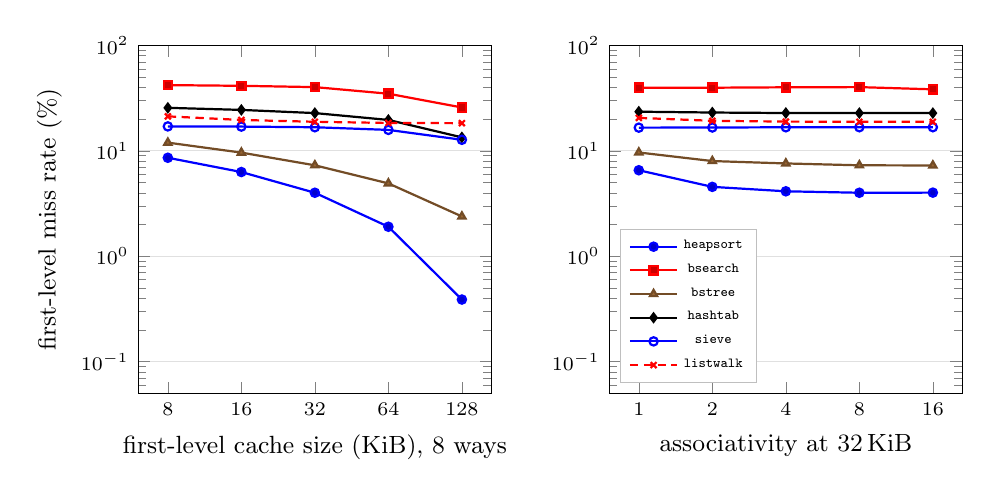
\begin{tikzpicture}
\begin{groupplot}[group style={group size=2 by 1, horizontal sep=1.5cm},
  width=0.50\linewidth, height=6.0cm, ymode=log, ymin=0.05, ymax=100,
  tick label style={font=\scriptsize}, label style={font=\small},
  ymajorgrids, grid style={draw=black!12}, legend style={font=\tiny, draw=black!25}]
\nextgroupplot[xmode=log, log basis x=2, xtick={8,16,32,64,128}, xticklabels={8,16,32,64,128}, xlabel={first-level cache size (KiB), 8 ways}, ylabel={first-level miss rate (\%)}]
\addplot+[mark=*, mark size=1.5pt, thick] coordinates {(8,8.6134) (16,6.3053) (32,4.0090) (64,1.9079) (128,0.3889)};
\addplot+[mark=square*, mark size=1.5pt, thick] coordinates {(8,42.1187) (16,41.4731) (32,40.3138) (64,34.9056) (128,25.8355)};
\addplot+[mark=triangle*, mark size=1.5pt, thick] coordinates {(8,11.9867) (16,9.6395) (32,7.3045) (64,4.9199) (128,2.3887)};
\addplot+[mark=diamond*, mark size=1.5pt, thick] coordinates {(8,25.6407) (16,24.5019) (32,22.8544) (64,19.6821) (128,13.4455)};
\addplot+[mark=o, mark size=1.5pt, thick] coordinates {(8,17.0834) (16,17.0143) (32,16.7775) (64,15.8294) (128,12.7560)};
\addplot+[mark=x, mark size=1.5pt, thick] coordinates {(8,21.2735) (16,19.6669) (32,18.9033) (64,18.4203) (128,18.3390)};
\nextgroupplot[xmode=log, log basis x=2, xtick={1,2,4,8,16}, xticklabels={1,2,4,8,16}, xlabel={associativity at 32\,KiB}, legend pos=south west]
\addplot+[mark=*, mark size=1.5pt, thick] coordinates {(1,6.5565) (2,4.5602) (4,4.1391) (8,4.0090) (16,4.0207)};
\addlegendentry{\texttt{heapsort}}
\addplot+[mark=square*, mark size=1.5pt, thick] coordinates {(1,39.8460) (2,39.8007) (4,40.1503) (8,40.3138) (16,38.4085)};
\addlegendentry{\texttt{bsearch}}
\addplot+[mark=triangle*, mark size=1.5pt, thick] coordinates {(1,9.6643) (2,8.0136) (4,7.6061) (8,7.3045) (16,7.2791)};
\addlegendentry{\texttt{bstree}}
\addplot+[mark=diamond*, mark size=1.5pt, thick] coordinates {(1,23.5565) (2,23.1365) (4,22.8866) (8,22.8544) (16,22.8490)};
\addlegendentry{\texttt{hashtab}}
\addplot+[mark=o, mark size=1.5pt, thick] coordinates {(1,16.6271) (2,16.6810) (4,16.7635) (8,16.7775) (16,16.7863)};
\addlegendentry{\texttt{sieve}}
\addplot+[mark=x, mark size=1.5pt, thick] coordinates {(1,20.5774) (2,19.3089) (4,18.9789) (8,18.9033) (16,18.8959)};
\addlegendentry{\texttt{listwalk}}
\end{groupplot}
\end{tikzpicture}
%% END GENERATED fig_l1sweep
\caption[First-level miss rate against size and associativity]{First-level
data-cache miss rate of six kernels in the model against cache size at eight ways (left) and
against associativity at 32\,KiB (right), both axes logarithmic. Halving the
cache is nearly free for some kernels and costly for others; the complete table
is in \Cref{app:results}.}
\label{fig:l1sweep}
\end{figure}

\begin{figure}[t]
\centering
%% BEGIN GENERATED fig_llcsweep
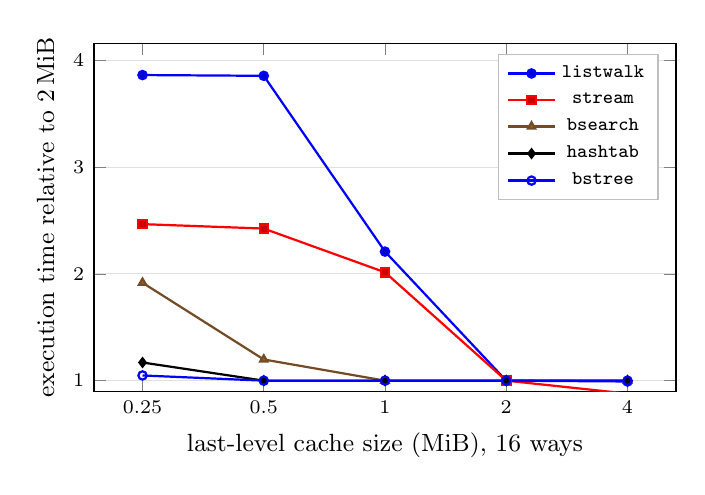
\begin{tikzpicture}
\begin{axis}[width=0.74\linewidth, height=6.0cm, xmode=log, log basis x=2,
  xtick={256,512,1024,2048,4096}, xticklabels={0.25,0.5,1,2,4},
  xlabel={last-level cache size (MiB), 16 ways}, ylabel={execution time relative to 2\,MiB},
  tick label style={font=\scriptsize}, label style={font=\small}, ymin=0.9,
  ymajorgrids, grid style={draw=black!12}, legend style={font=\scriptsize, draw=black!25},
  legend pos=north east]
\addplot+[mark=*, mark size=1.5pt, thick] coordinates {(256,3.8626) (512,3.8554) (1024,2.2090) (2048,1.0000) (4096,0.9924)};
\addlegendentry{\texttt{listwalk}}
\addplot+[mark=square*, mark size=1.5pt, thick] coordinates {(256,2.4662) (512,2.4247) (1024,2.0149) (2048,1.0000) (4096,0.8787)};
\addlegendentry{\texttt{stream}}
\addplot+[mark=triangle*, mark size=1.5pt, thick] coordinates {(256,1.9172) (512,1.1984) (1024,1.0000) (2048,1.0000) (4096,1.0000)};
\addlegendentry{\texttt{bsearch}}
\addplot+[mark=diamond*, mark size=1.5pt, thick] coordinates {(256,1.1701) (512,1.0000) (1024,1.0000) (2048,1.0000) (4096,1.0000)};
\addlegendentry{\texttt{hashtab}}
\addplot+[mark=o, mark size=1.5pt, thick] coordinates {(256,1.0488) (512,1.0000) (1024,1.0000) (2048,1.0000) (4096,1.0000)};
\addlegendentry{\texttt{bstree}}
\end{axis}
\end{tikzpicture}
%% END GENERATED fig_llcsweep
\caption[Execution time against last-level cache size]{Execution time of five
kernels in the model against the size of the last-level cache, relative to the 2\,MiB
default. \code{listwalk}, whose list occupies 1\,MiB, runs
\R{llc.half.listwalk}\pc{} longer when the cache is halved and
\R{llc.quarter.listwalk}\pc{} longer when it is quartered; kernels whose
working set fits either way are unaffected.}
\label{fig:llcsweep}
\end{figure}

The shape in \Cref{fig:llcsweep} is a cliff, not a slope: a kernel is
indifferent to capacity until its working set no longer fits, and then pays
heavily. This is the single most useful fact for reading the isolation results
of \Cref{ch:tradeoffs}.

\section{The measurement primitives}
\label{sec:primitives}

\Cref{fig:primitives} contrasts the two most important ways of observing a
cache, and \Cref{tab:primitives} compares the four that the literature
established.

\begin{figure}[t]
\centering
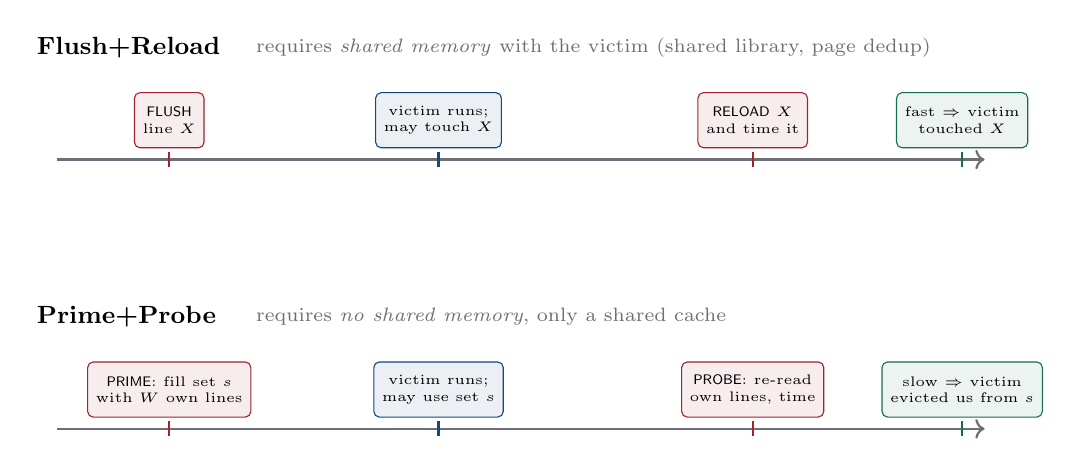
\begin{tikzpicture}[scale=0.95, every node/.style={font=\scriptsize}]
  % ---------- Flush+Reload ----------
  \node[anchor=west, font=\small\bfseries] at (-0.4,2.1) {Flush+Reload};
  \node[note, anchor=west] at (2.6,2.1) {requires \emph{shared memory} with the victim
       (shared library, page dedup)};
  \draw[->, thick, muted] (0,0.6) -- (12.4,0.6);
  \foreach \x/\lab/\c in {0.6/{\textsf{FLUSH}\\line $X$}/attack,
                          4.2/{victim runs;\\may touch $X$}/accent,
                          8.4/{\textsf{RELOAD} $X$\\and time it}/attack,
                          11.2/{fast $\Rightarrow$ victim\\touched $X$}/defense}
     {\node[draw=\c, fill=\c!8, rounded corners=2pt, minimum height=7mm, inner sep=3pt,
            align=center, font=\tiny, anchor=south] at (\x+0.9,0.75) {\lab};
      \draw[\c, thick] (\x+0.9,0.5) -- (\x+0.9,0.7);}
  % ---------- Prime+Probe ----------
  \node[anchor=west, font=\small\bfseries] at (-0.4,-1.5) {Prime+Probe};
  \node[note, anchor=west] at (2.6,-1.5) {requires \emph{no shared memory}, only a shared cache};
  \draw[->, thick, muted] (0,-3.0) -- (12.4,-3.0);
  \foreach \x/\lab/\c in {0.6/{\textsf{PRIME}: fill set $s$\\with $W$ own lines}/attack,
                          4.2/{victim runs;\\may use set $s$}/accent,
                          8.4/{\textsf{PROBE}: re-read\\own lines, time}/attack,
                          11.2/{slow $\Rightarrow$ victim\\evicted us from $s$}/defense}
     {\node[draw=\c, fill=\c!8, rounded corners=2pt, minimum height=7mm, inner sep=3pt,
            align=center, font=\tiny, anchor=south] at (\x+0.9,-2.85) {\lab};
      \draw[\c, thick] (\x+0.9,-3.1) -- (\x+0.9,-2.9);}
\end{tikzpicture}
\caption[Flush+Reload and Prime+Probe]{The two canonical cache measurement
primitives. Flush+Reload~\citep{yarom2014flushreload} is precise (line
granularity, low noise) but needs memory shared with the victim.
Prime+Probe~\citep{osvik2006cache,liu2015llc} needs no sharing at all and
therefore works across processes and across cores, at the cost of set-granular
resolution and more noise.}
\label{fig:primitives}
\end{figure}

\begin{table}[t]
\centering
\caption[Comparison of cache measurement primitives]{The four principal cache
measurement primitives, with the attacker scenarios of \Cref{tab:threat} in
which each has been demonstrated. ``Shared memory'' means that observer and
victim map the same physical page.}
\label{tab:primitives}
\footnotesize
\begin{tabularx}{\linewidth}{@{}>{\raggedright\arraybackslash}p{2.9cm}p{1.2cm}>{\raggedright\arraybackslash}p{2.9cm}X@{}}
\toprule
\textbf{Primitive} & \textbf{Scen.} & \textbf{Requires} & \textbf{Characteristics} \\
\midrule
Evict+Time \newline \citep{osvik2006cache} & S2 &
Ability to trigger the victim &
Times the victim's own run after displacing a set. Coarse; historically the
first. \\
\addlinespace
Prime+Probe \newline \citep{osvik2006cache,liu2015llc} & S2, S3 &
A shared cache &
Resolves activity to a set. Works across cores on a shared last-level cache.
Needs an eviction set for the set observed. \\
\addlinespace
Flush+Reload \newline \citep{yarom2014flushreload} & S2, S3 &
Shared memory and a way to evict a chosen line &
Resolves activity to a line, with little noise. On RISC-V the eviction is
\code{cbo.flush} where user mode may execute it, or displacement otherwise. \\
\addlinespace
Flush+Flush \newline \citep{gruss2016flushflush} & S2, S3 &
Shared memory and a flush instruction &
Times the flush instead of a reload, so the observer itself causes no
additional misses. \\
\bottomrule
\end{tabularx}
\end{table}

\Cref{lst:primeprobe} states Prime+Probe as pseudocode. Its first line hides the
main cost: finding an \emph{eviction set}, a group of $W$ of the observer's own\index{eviction set}
lines that map to the set of interest. For a first-level cache indexed with
bits of the page offset this is immediate. For a physically indexed last-level
cache the observer does not know its physical addresses and has to find
conflicting lines by experiment; the number of memory accesses needed is linear
in the size of the candidate pool with the best known
methods~\citep{vila2019theory}. This search is the step that randomised caches
(\Cref{sec:randomisation}) are designed to defeat.

\begin{lstlisting}[language=pseudo, caption={Prime+Probe on one cache set, as
pseudocode. $W$ is the associativity of the cache.}, label={lst:primeprobe}]
procedure PrimeProbe(set s)
    E = W lines of the observer that all map to set s   // the eviction set
    repeat
        access every line in E          // prime: set s now holds only E
        wait while the other party runs
        t = time to access every line in E again        // probe
        if t > threshold then record "set s was used in this round"
    until enough rounds are recorded
    combine the rounds, for example by majority vote
\end{lstlisting}

How reliable one such observation is depends on how far apart the hit and miss
latencies are compared with the noise of the timer. \Cref{app:leakage} models
the decision as a binary channel and tabulates the error rate, the capacity per
observation and the number of repetitions needed for a given reliability.
Coarsening the timer raises the number of repetitions; it does not remove the
difference being measured.

\section{Virtual memory and the translation path}
\label{sec:vm}

Textbook \SecRef{11.4} introduces virtual memory, \SecRef{11.4.3} paging, and
\SecRef{11.4.5} the memory management unit that caches recent translations in a\index{memory management unit (MMU)}
TLB. RISC-V uses a radix page table walked by hardware~\citep{riscv-priv};
\Cref{fig:sv39} shows the path, and \Cref{app:priv} works through a walk.

\begin{figure}[t]
\centering
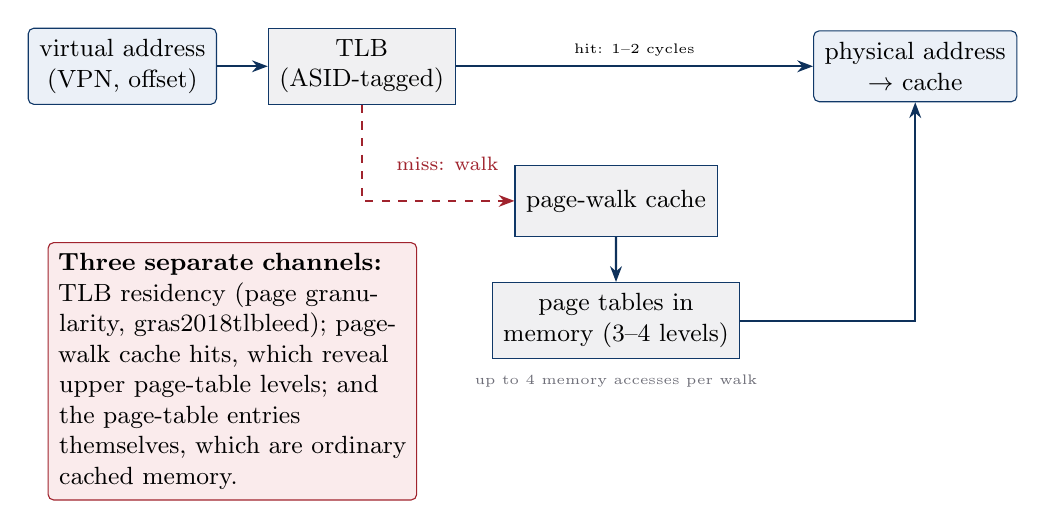
\begin{tikzpicture}[scale=0.95, every node/.style={font=\scriptsize}]
  \node[blk, minimum width=2.0cm, minimum height=0.9cm] (va) at (0,0) {virtual address\\(VPN, offset)};
  \node[memblk, minimum width=1.7cm, minimum height=0.9cm] (tlb) at (3.2,0) {TLB\\(ASID-tagged)};
  \node[blk, minimum width=1.9cm, minimum height=0.9cm] (pa) at (10.6,0) {physical address\\$\rightarrow$ cache};
  \node[memblk, minimum width=1.9cm, minimum height=0.9cm] (pwc) at (6.6,-1.8) {page-walk cache};
  \node[memblk, minimum width=1.9cm, minimum height=0.9cm] (pt) at (6.6,-3.4) {page tables in\\memory (3--4 levels)};

  \draw[sig] (va) -- (tlb);
  \draw[sig] (tlb) -- node[above, font=\tiny] {hit: 1--2 cycles} (pa);
  \draw[atksig] (tlb.south) |- (pwc.west);
  \node[note, anchor=north west, text=attack] at (3.6,-1.15) {miss: walk};
  \draw[sig] (pwc) -- (pt);
  \draw[sig] (pt.east) -| (pa.south);
  %% below the page-table box: the gap between it and the riser is too narrow
  \node[font=\tiny, anchor=north, text=muted] at (6.6,-4.0)
        {up to 4 memory accesses per walk};

  \node[atk, text width=4.4cm, align=left, anchor=north west] at (-1.0,-2.35)
    {\textbf{Three separate channels:} TLB residency (page granularity,
     \citep{gras2018tlbleed}); page-walk cache hits, which reveal upper
     page-table levels; and the page-table entries

     themselves, which are ordinary cached memory.};
\end{tikzpicture}
\caption[Address translation and its channels]{The RISC-V Sv39 translation path
(\SecRef{11.4.3}, \SecRef{11.4.5}). Each structure on the path keeps state of its
own: the TLB, the page-walk cache, and the page-table entries, which are
ordinary memory and are cached like any other. The address-space identifier
that tags TLB entries is defined by the privileged
architecture~\citep{riscv-priv}.}
\label{fig:sv39}
\end{figure}

The TLB resolves activity to a page, not to a line, but it is a separate\index{translation-lookaside buffer (TLB)!as a channel}
structure with separate contents, and a defence that flushes or partitions the
data caches does not thereby cover it. Gras \etal{} used exactly this to
observe a victim through the TLB on a system whose caches were
protected~\citep{gras2018tlbleed}. Translation is also a cost in its own right:
in the model \code{listwalk} misses its 32-entry TLB on
\R{base.listwalk.tlb_miss_pct}\pc{} of its accesses.

\begin{takeaway}
The memory system offers a family of channels at different granularities: line
(the caches), page (the TLB), page-table level (the walk cache), DRAM row (the\index{page-walk cache}
row buffer~\citep{pessl2016drama}), and the tables of the prefetcher, which
Gruss \etal{} used to learn about address
translation~\citep{gruss2016prefetch}. A defence scoped to one member of the
family does not constrain the others. This is the strongest argument for the
defences of \Cref{sec:taint}, which reason about information flow instead of
about one structure.
\end{takeaway}


\chapter{Multicore Systems: Sharing, Coherence and Cross-Domain Leakage}
\label{ch:multicore}

\begin{tocmapbox}
Background: textbook \SecRef{12.2} (software for multiprocessor systems,
including Amdahl's law in \SecRef{12.2.3}), \SecRef{12.3} (the design space of
multiprocessors), and \SecRef{12.4} (MIMD multiprocessors) with
\SecRef{12.4.1} (logical point of view), \SecRef{12.4.2} (coherence),
\SecRef{12.4.3} (memory consistency), \SecRef{12.4.4} (physical view of memory),
\SecRef{12.4.5} (shared caches), \SecRef{12.4.6} (coherent private caches) and
\SecRef{12.4.8} (multithreaded processors)~\citep{sarangi2025basic}.
\end{tocmapbox}

\section{What sharing adds}

So far the observer and the victim have taken turns on one core. In a multicore
system the observer can run \emph{at the same time} as the victim, on another
core, and still share the last-level cache, the interconnect, the memory
controller and DRAM. This is scenario S3 of \Cref{tab:threat}, the one that
matters commercially because it is the setting of cloud co-tenancy.
\Cref{fig:multicore} shows the organisation of \SecRef{12.3}--\SecRef{12.4.4}
for a four-core system.

\begin{figure}[t]
\centering
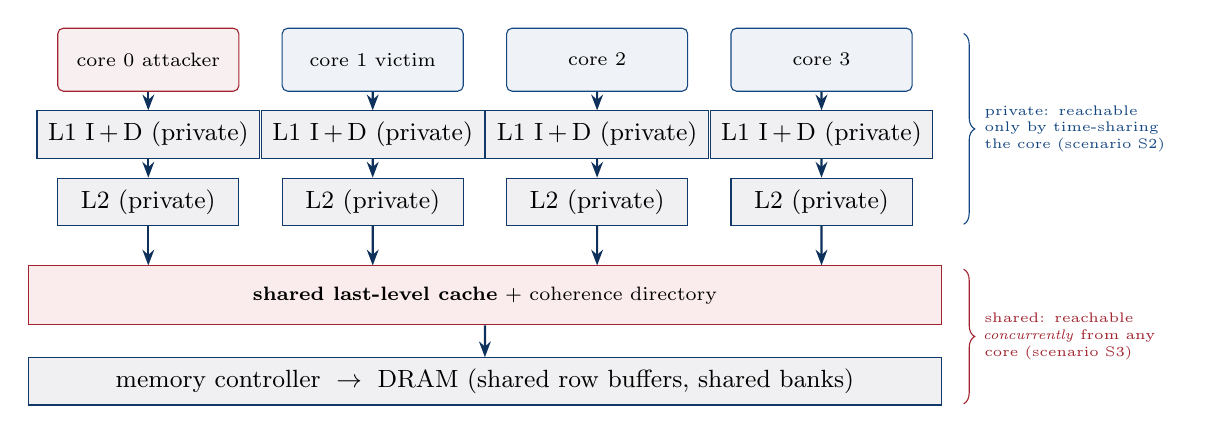
\begin{tikzpicture}[scale=0.95, every node/.style={font=\scriptsize}]
  \foreach \i/\x/\owner/\col in {0/0/attacker/attack, 1/3.0/victim/accent,
                                 2/6.0/{}/accent, 3/9.0/{}/accent}
  {
    \node[draw=\col, fill=\col!7, rounded corners=2pt, minimum width=2.3cm,
          minimum height=0.8cm] (c\i) at (\x,2.6) {core \i\ \owner};
    \node[memblk, minimum width=2.3cm, minimum height=0.6cm] (l1\i) at (\x,1.6) {L1 I\,+\,D (private)};
    \node[memblk, minimum width=2.3cm, minimum height=0.6cm] (l2\i) at (\x,0.7) {L2 (private)};
    \draw[sig] (c\i) -- (l1\i); \draw[sig] (l1\i) -- (l2\i);
    \draw[sig] (l2\i) -- (\x,-0.15);
  }
  \node[draw=attack, fill=attackfill, minimum width=11.6cm, minimum height=0.75cm]
       (llc) at (4.5,-0.55) {\textbf{shared last-level cache} + coherence directory};
  \node[memblk, minimum width=11.6cm, minimum height=0.6cm] (mc) at (4.5,-1.7)
       {memory controller \;$\rightarrow$\; DRAM (shared row buffers, shared banks)};
  \draw[sig] (llc) -- (mc);

  \draw[decorate, decoration={brace, amplitude=4pt}, accent]
       (10.9,2.95) -- (10.9,0.4)
       node[midway, right=4pt, align=left, text width=2.35cm, font=\tiny]
       {private: reachable only by time-sharing the core (scenario S2)};
  \draw[decorate, decoration={brace, amplitude=4pt}, attack]
       (10.9,-0.2) -- (10.9,-2.0)
       node[midway, right=4pt, align=left, text width=2.35cm, font=\tiny, text=attack]
       {shared: reachable \emph{concurrently} from any core (scenario S3)};

\end{tikzpicture}
\caption[Multicore sharing]{A four-core RISC-V system (\SecRef{12.4.4},
\SecRef{12.4.5}, \SecRef{12.4.6}). Private
caches require the attacker to time-share a core; the LLC, the directory, the
interconnect and DRAM are shared continuously. An \emph{inclusive} LLC couples
the two regions: evicting a line from the LLC forces its eviction from another
core's private L1, which is what makes cross-core Prime+Probe
practical~\citep{liu2015llc}.}
\label{fig:multicore}
\end{figure}

\section{Coherence as a channel}
\label{sec:coherence}

Textbook \SecRef{12.4.2} develops cache coherence, the invariant that all cores\index{cache coherence!MESI protocol}
observe a single value for each memory location, and \SecRef{12.4.6} applies it
to coherent private caches. \Cref{fig:mesi} shows the MESI states; the protocol
is walked through transition by transition in
\Cref{app:coherence}~\citep{nagarajan2020primer}.

\begin{figure}[t]
\centering
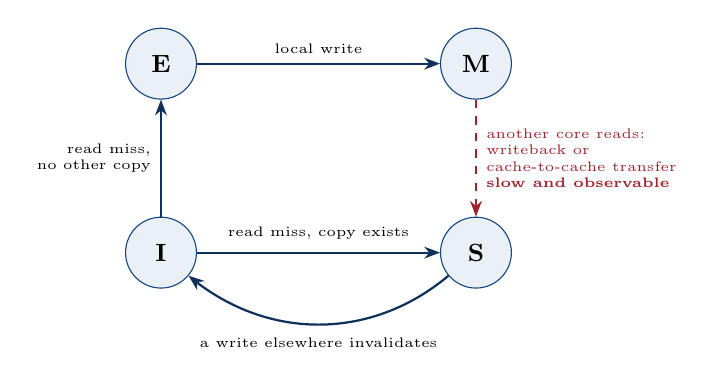
\begin{tikzpicture}[scale=1.0, every node/.style={font=\scriptsize},
                    st/.style={draw=accent, fill=lightfill, circle, minimum size=9mm,
                               font=\small\bfseries}]
  \node[st] (i) at (0,0)   {I};
  \node[st] (e) at (0,2.4) {E};
  \node[st] (m) at (4.0,2.4) {M};
  \node[st] (s) at (4.0,0) {S};
  \draw[sig] (i) -- node[left, font=\tiny, align=right]
        {read miss,\\no other copy} (e);
  \draw[sig] (e) -- node[above, font=\tiny] {local write} (m);
  \draw[atksig] (m) -- node[right, font=\tiny, align=left, text=attack]
        {another core reads:\\writeback or\\cache-to-cache transfer\\\textbf{slow and observable}} (s);
  %% bowed below so the label clears both state circles
  \draw[sig] (s) to[out=-140,in=-40] node[below=1pt, font=\tiny, pos=0.5]
        {a write elsewhere invalidates} (i);
  \draw[sig] (i) -- node[above=1pt, font=\tiny, pos=0.5]
        {read miss, copy exists} (s);
\end{tikzpicture}
\par\vspace{4pt}
\begin{tcolorbox}[enhanced, width=0.92\linewidth, colback=attackfill, colframe=attack,
  boxrule=0.4pt, arc=2pt, left=7pt, right=7pt, top=5pt, bottom=5pt, fontupper=\small]
\textbf{Why this is a channel.} Coherence transitions have different costs.
Reading a line that another core holds in M requires a writeback or a
cache-to-cache transfer and is measurably slower than reading a line in S. The
attacker therefore learns not only \emph{whether} the victim touched a line, but
\emph{whether it wrote to it}, a strictly stronger observation than the plain
cache-state channel of \Cref{ch:memsys}.
\end{tcolorbox}
\caption[MESI states and their timing]{The MESI coherence protocol
(\SecRef{12.4.2}, \SecRef{12.4.6}) and the transitions that create a channel. Coherence is a
correctness mechanism; the timing asymmetry between its transitions is an
unintended, and unavoidable, side effect.}
\label{fig:mesi}
\end{figure}

Two consequences follow from the fact that transitions differ in cost.
\textbf{Reads can be told from writes.} A read of a line that another core\index{cache coherence!read/write discrimination}
holds in Modified state needs a transfer from that core and takes longer than
a read of a line in Shared state, so an observer with access to a shared line
learns whether the other party wrote to it. \textbf{Invalidation is itself a
signal.} A write by one core invalidates the copies held by others, and an\index{cache coherence!invalidation as transmitter}
observer that held a copy sees its next access miss. Neither effect needs an
eviction or any pressure on capacity.

\section{Memory consistency and fences}

\SecRef{12.4.3} covers memory consistency, the rules governing the order in
which one core's memory operations become visible to others.\index{memory consistency!RVWMO} RISC-V specifies
the RVWMO model, in which \code{fence} constrains that
order~\citep{riscv-unpriv}. For this paper the relevant point is negative:
\textbf{a memory fence is an ordering instruction.}\index{fence instruction!ordering versus erasure} It does not remove cache
lines, TLB entries or predictor state, and the specification does not define it
as a barrier to speculative execution. Whether a particular instruction happens
to serialise the pipeline on a particular core is a property of that core; the
measurements on commercial RISC-V cores discussed in \Cref{ch:transient} found
no cheap, portable barrier. The \code{fence.t} proposal exists because erasure
is a different operation from ordering.

\section{Simultaneous multithreading}

When two hardware threads share one core (\SecRef{12.4.8}), they share the\index{simultaneous multithreading (SMT)}
first-level caches, the TLB, the predictors and the execution ports, at the
same time and not in alternation. Contention for a port can be observed at\index{port contention}
cycle granularity without any change of cache state~\citep{aldaya2019port}.
The open RISC-V cores discussed in this paper are single-threaded, so this
surface does not arise on them; it would arrive with multithreading.

\begin{takeaway}
Every sharing decision in \Cref{fig:multicore} is a performance decision that
also defines who can observe whom. An inclusive last-level cache simplifies
coherence \emph{and} couples the private caches of different cores.
ASID-tagged TLBs avoid flushes \emph{and} keep another address space's entries
resident. Multithreading raises throughput \emph{and} shares execution ports.
\end{takeaway}

\section{Partitioning and colouring}
\label{sec:partitioning}

The textbook explains why caches are shared (\SecRef{12.4.5},
\SecRef{12.4.6}). Dividing them again between security domains is not textbook
material; it comes from the research literature and is the oldest hardware
defence against cache channels. \Cref{fig:partition} contrasts the two
mechanisms, and \Cref{app:isolation} gives the details of each.

\begin{figure}[t]
\centering
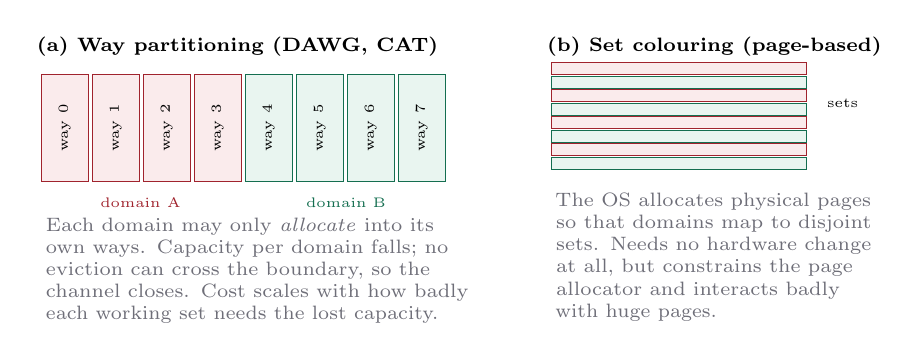
\begin{tikzpicture}[scale=0.9, every node/.style={font=\tiny}]
  % --- way partitioning ---
  \node[font=\scriptsize\bfseries, anchor=west] at (-0.2,3.1) {(a) Way partitioning (DAWG, CAT)};
  \foreach \w in {0,...,7}{
    \pgfmathsetmacro{\xx}{\w*0.72}
    \ifnum\w<4
      \draw[fill=attackfill, draw=attack] (\xx,1.2) rectangle ++(0.66,1.5);
    \else
      \draw[fill=defensefill, draw=defense] (\xx,1.2) rectangle ++(0.66,1.5);
    \fi
    \node[rotate=90] at (\xx+0.33,1.95) {way \w};}
  \node[anchor=north, text=attack] at (1.4,1.1) {domain A};
  \node[anchor=north, text=defense] at (4.3,1.1) {domain B};
  \node[note, anchor=north west, text width=5.4cm] at (0,0.75)
    {Each domain may only \emph{allocate} into its own ways. Capacity per domain
     falls; no eviction can cross the boundary, so the channel closes. Cost scales
     with how badly each working set needs the lost capacity.};

  % --- set partitioning / colouring ---
  \node[font=\scriptsize\bfseries, anchor=west] at (7.0,3.1) {(b) Set colouring (page-based)};
  \foreach \s in {0,...,7}{
    \pgfmathsetmacro{\yy}{2.7-\s*0.19}
    \ifodd\s
      \draw[fill=defensefill, draw=defense] (7.2,\yy) rectangle ++(3.6,0.17);
    \else
      \draw[fill=attackfill, draw=attack] (7.2,\yy) rectangle ++(3.6,0.17);
    \fi}
  \node[anchor=west] at (10.95,2.3) {sets};
  \node[note, anchor=north west, text width=4.0cm] at (7.2,1.1)
    {The OS allocates physical pages so that domains map to disjoint sets. Needs
     no hardware change at all, but constrains the page allocator and interacts
     badly with huge pages.};
\end{tikzpicture}
\caption[Two partitioning mechanisms]{Way partitioning and set colouring,
applied to the shared caches of \SecRef{12.4.5}. Both remove the possibility
that one domain displaces another's lines, and both pay for it in the capacity
left to each domain.}
\label{fig:partition}
\end{figure}

\textbf{Way partitioning} gives each domain a subset of the ways of every set.\index{cache partitioning!way partitioning}
It needs hardware support and limits the number of domains to the
associativity. DAWG~\citep{kiriansky2018dawg} is the worked-out design: it
isolates hits and replacement metadata as well as fills. Cache allocation
technology on commercial processors restricts fills only, and
CATalyst~\citep{liu2016catalyst} builds a defence on it.

\textbf{Page colouring} needs no hardware. The operating system hands each\index{page colouring}
domain physical pages whose frame numbers differ in the bits that take part in
the cache index, so that the domains occupy disjoint sets~\citep{kessler1992page}.
The number of colours a cache offers is the size of one of its ways divided by
the page size, and this arithmetic decides where colouring works:
\begin{itemize}
  \item a 32\,KiB eight-way first-level cache has ways of 4\,KiB, one colour:
        it cannot be coloured at all with 4\,KiB pages;
  \item the 256\,KiB eight-way second level of the model has 8 colours and its
        2\,MiB sixteen-way last level has 32;
  \item with 2\,MiB pages neither has any, because a page then covers every
        set. Large pages do not break colouring in principle; they remove the
        index bits that colouring uses for caches of this size.
\end{itemize}
A complete spatial defence therefore colours the outer caches and treats the
first-level cache, the TLB and the predictors separately, by flushing them at a
switch or by partitioning them.

\section{What isolation removes: results from the model}
\label{sec:interference}

The model of \Cref{ch:study} can run two kernels as two security domains that
alternate on one core. It counts, per context switch, how often a fill by one
domain displaces a line of the other, how often a prediction is made from an
entry that the other domain wrote, and how much state the outgoing domain
leaves in each structure. These counts are not an attack. They measure the
\emph{opportunity} for one: a channel between the domains needs at least one of
them to be non-zero. \Cref{tab:interference} gives them for five pairs of
kernels switching every \num{100000} instructions.

\begin{table}[t]
\centering
\caption[Cross-domain interference under each isolation mechanism]{Interference
between two domains sharing one core in the model, per context switch, averaged over five
pairs of kernels and five page-frame layouts. Left: lines of one domain evicted
by the other from each cache and from the TLB, and predictions made from the
other domain's entries. Right: valid entries the outgoing domain leaves behind
in the first-level data cache, the TLB, the BTB and the pattern table.
\emph{Flush} clears first-level caches, TLB and predictors at each switch;
\emph{Colour} assigns page frames by parity; \emph{WayPart} halves every cache,
the TLB and the predictor tables; \emph{RandLLC} encrypts the last-level
index.}
\label{tab:interference}
\footnotesize
%% BEGIN GENERATED tab_interference
\begin{tabular}{@{}l@{\hspace{10pt}}rrrrr@{\hspace{14pt}}rrrr@{}}
\toprule
 & \multicolumn{5}{c}{\textbf{cross-domain evictions and uses}} & \multicolumn{4}{c}{\textbf{state left behind}} \\
\textbf{Mechanism} & \textbf{L1D} & \textbf{L2} & \textbf{LLC} & \textbf{TLB} & \textbf{Pred.} & \textbf{L1D} & \textbf{TLB} & \textbf{BTB} & \textbf{PHT} \\
\midrule
No isolation & 329 & 693 & 16 & 13 & 3 & 421 & 22 & 7 & 257 \\
\midrule
Flush & 0 & 694 & 16 & 0 & 0 & 0 & 0 & 0 & 0 \\
Flush+Colour & 0 & 0 & 0 & 0 & 0 & 0 & 0 & 0 & 0 \\
Colour & 329 & 0 & 0 & 13 & 3 & 421 & 22 & 7 & 257 \\
WayPart & 0 & 0 & 0 & 0 & 0 & 256 & 15 & 7 & 188 \\
RandLLC & 329 & 693 & 17 & 13 & 3 & 421 & 22 & 7 & 257 \\
\bottomrule
\end{tabular}
%% END GENERATED tab_interference
\end{table}

\begin{finding}
Without isolation a domain evicts on average
\R{inter.shared.l1d_cross_evictions} first-level lines and
\R{inter.shared.l2_cross_evictions} second-level lines of the other per switch
and finds \R{inter.shared.residue_l1d} of the 512 first-level lines still
holding the other's data. Flushing removes the on-core part and leaves the
outer caches untouched; colouring removes the outer part and leaves the core
untouched; only the combination, or partitioning of every structure, brings
all interference counts to zero. A randomised last-level index leaves every
count where it was: it does not stop one domain displacing the other, it stops
the displacement being \emph{aimed}.
\end{finding}

The last row is a caution about the metric as much as about the mechanism.
Randomisation is designed to make evictions unpredictable, and a count of
evictions cannot show that. Its effect has to be argued from the cost of
finding conflicting lines, which is done analytically in \Cref{app:random}.


\chapter{Transient Execution Attacks}
\label{ch:transient}

This chapter has no single textbook counterpart, because transient-execution
attacks are more recent than most textbook treatments of pipelining. It is
built from \Cref{ch:pipeline} (speculation, squashing, precise exceptions, the
execution window) and \Cref{ch:memsys} (the cache as the place where a trace is
left and read). It describes the attacks at the level needed to understand the
defences and reports what has been demonstrated on RISC-V; it does not develop
attack code.

\section{Anatomy}

Every transient-execution attack has the four phases of \Cref{fig:anatomy},\index{transient execution!four phases}
following the systematisation of Canella \etal~\citep{canella2019systematic}.
In the \emph{setup} the attacker arranges for the core to mispredict or to
fault. In the \emph{access} phase the core transiently reads data. What makes
that data sensitive differs between the two families. In a Spectre attack the
victim is architecturally entitled to read it, and it is the victim's own
program logic, a bounds check for example, that is bypassed for the duration
of the misprediction. In a Meltdown-type attack the read is one that a
permission check forbids, and the data reaches later instructions before the
fault is taken. In the \emph{transmit} phase a transient instruction changes
\uarchadj{} state in a way that depends on the data, and in the \emph{receive}
phase that state is measured with one of the primitives of
\Cref{sec:primitives}.

\begin{figure}[t]
\centering
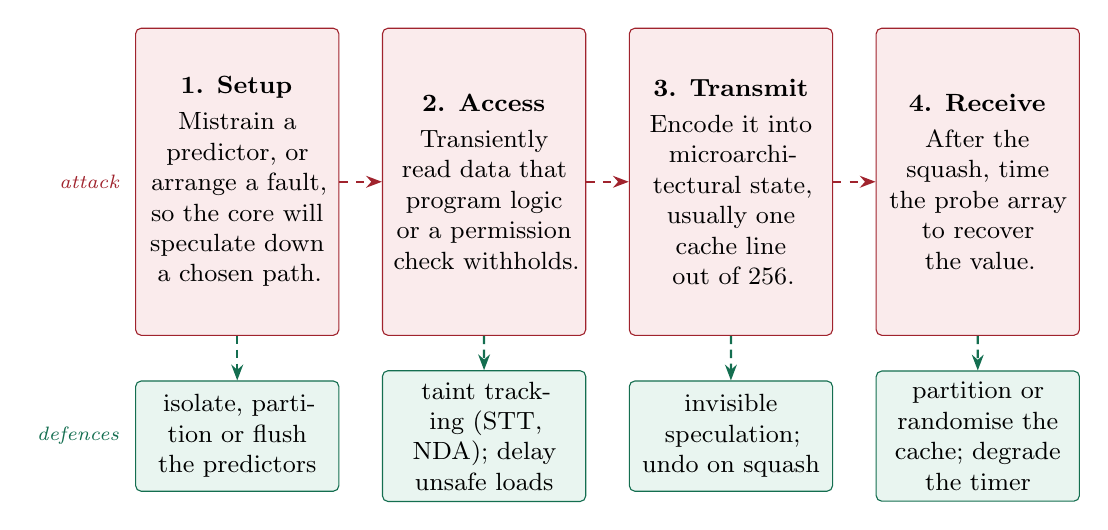
\begin{tikzpicture}[scale=0.95, every node/.style={font=\scriptsize}]
  \node[atk, minimum width=2.5cm, minimum height=3.9cm, text width=2.3cm] (p1) at (0,0)
       {\textbf{1. Setup}\\[2pt] Mistrain a predictor, or arrange a fault, so the core
        will speculate down a chosen path.};
  \node[atk, minimum width=2.5cm, minimum height=3.9cm, text width=2.3cm] (p2) at (3.3,0)
       {\textbf{2. Access}\\[2pt] Transiently read data that program logic or a
        permission check withholds.};
  \node[atk, minimum width=2.5cm, minimum height=3.9cm, text width=2.3cm] (p3) at (6.6,0)
       {\textbf{3. Transmit}\\[2pt] Encode it into \uarchadj{} state, usually one
        cache line out of 256.};
  \node[atk, minimum width=2.5cm, minimum height=3.9cm, text width=2.3cm] (p4) at (9.9,0)
       {\textbf{4. Receive}\\[2pt] After the squash, time the probe array to
        recover the value.};
  \foreach \a/\b in {p1/p2, p2/p3, p3/p4} {\draw[atksig] (\a) -- (\b);}

  \node[def, minimum width=2.5cm, text width=2.3cm, minimum height=1.4cm] (d1) at (0,-3.4)
       {isolate, partition or flush the predictors};

  \node[def, minimum width=2.5cm, text width=2.3cm, minimum height=1.4cm] (d2) at (3.3,-3.4)
       {taint tracking (STT, NDA); delay unsafe loads};
  \node[def, minimum width=2.5cm, text width=2.3cm, minimum height=1.4cm] (d3) at (6.6,-3.4)
       {invisible speculation; undo on squash};
  \node[def, minimum width=2.5cm, text width=2.3cm, minimum height=1.4cm] (d4) at (9.9,-3.4)
       {partition or randomise the cache; degrade the timer};
  \foreach \a/\b in {p1/d1, p2/d2, p3/d3, p4/d4} {\draw[defsig, densely dashed] (\a) -- (\b);}
  \node[anchor=east, font=\scriptsize\itshape, text=attack]  at (-1.45,0)    {attack};
  \node[anchor=east, font=\scriptsize\itshape, text=defense] at (-1.45,-3.4) {defences};
\end{tikzpicture}
\caption[Anatomy of a transient-execution attack]{The four phases of a
transient-execution attack, and the defence class that targets each. The
taxonomy of \Cref{ch:defenses} is organised by which phase a mechanism attacks,
because that determines what it can and cannot cover.}
\label{fig:anatomy}
\end{figure}

Naming the phases separately is useful because different defences act on
different phases. It does not follow that two defences acting on different
phases compose, or that two acting on the same phase are redundant; whether a
combination is sound depends on the assumptions each makes, and
\Cref{sec:composition} looks at what a combination costs.

\section{Spectre-v1: bounds-check bypass}

\Cref{lst:spectre1} is the code pattern from which the family takes its
name~\citep{kocher2019spectre}. The bounds check is correct: architecturally,\index{Spectre!v1, bounds-check bypass}
\code{x} is never out of range when the body runs. If the branch has recently
been taken many times with in-range values, the direction predictor predicts
it taken again, and for an out-of-range \code{x} the core executes the body
transiently until the comparison resolves.

\begin{lstlisting}[language=C, caption={The Spectre-v1 gadget in C. Phases 1--3
of \Cref{fig:anatomy} all occur inside these three lines; phase 4 happens in the
attacker's own code afterwards.}, label={lst:spectre1}]
if (x < array1_size) {          /* mistrained: predicted TAKEN  */
    uint8_t v = array1[x];      /* transient out-of-bounds read */
    temp &= array2[v * 512];    /* transmit: 1 line out of 256  */
}
\end{lstlisting}

\Cref{lst:spectre1rv} writes the same pattern in RISC-V assembly, for
illustration; it is not compiler output. Nothing in the RISC-V encoding, the
privilege model or the memory model prohibits any instruction in it. The two
loads are exactly the dependent pair of \Cref{lst:leak}, and
\Cref{tab:window} showed that such pairs also occur transiently in ordinary
code.

\begin{lstlisting}[language=riscv, caption={The same gadget in RISC-V assembly.
The branch at line~2 is the one that is mistrained; lines 3--9 are the transient
window; line~9 is the transmitter.}, label={lst:spectre1rv}]
  ld    t0, array1_size      # bound
  bgeu  a0, t0, .Lskip       # mistrained: predicted NOT taken
  la    t1, array1
  add   t1, t1, a0           # transiently computes an out-of-bounds address
  lbu   t2, 0(t1)            # transient read of forbidden data -> t2
  slli  t2, t2, 9            # scale by 512 bytes
  la    t3, array2
  add   t3, t3, t2
  lbu   t4, 0(t3)            # TRANSMIT: allocates one of 256 cache lines
.Lskip:
  ret                        # reached on both paths
\end{lstlisting}

\begin{takeaway}
Spectre-v1 needs no privilege escalation, no fault and no architectural bug:
only a mispredicted branch, a window long enough for two dependent loads, and
a cache. The mechanism exploited is the performance mechanism, which is why
the defences of \Cref{ch:defenses} cost performance.
\end{takeaway}

\section{The variant family}

\Cref{tab:variants} organises the main variants by the mechanism each relies
on, and summarises the evidence on RISC-V, which \Cref{tab:rvevidence} gives
in detail.

\begin{table}[t]
\centering
\caption[Transient-execution variants]{The principal transient-execution
variants, the mechanism each relies on, and the evidence for RISC-V cores in
the studies of \Cref{tab:rvevidence}. ``Silicon'' refers to the commercial
cores measured by Gerlach \etal~\citep{gerlach2026spectre}.}
\label{tab:variants}
\footnotesize
\begin{tabularx}{\linewidth}{@{}>{\raggedright\arraybackslash}p{2.8cm}>{\raggedright\arraybackslash}p{4.0cm}X@{}}
\toprule
\textbf{Variant} & \textbf{Mechanism} & \textbf{Evidence on RISC-V} \\
\midrule
Spectre-v1, bounds-check bypass \citep{kocher2019spectre} &
Mistrained direction predictor; transient out-of-bounds load &
Demonstrated on BOOM in cycle-exact simulation~\citep{gonzalez2019replicating}
and on silicon (XuanTie C910, SiFive P550). \\
\addlinespace
Spectre-v2, branch target injection \citep{kocher2019spectre} &
A target predicted from an entry written by other code redirects transient
execution &
Demonstrated on BOOM~\citep{gonzalez2019replicating,balucea2023software} and on
silicon, where the firmware of some boards ships with the target predictor
disabled. \\
\addlinespace
Spectre-RSB \citep{koruyeh2018spectre}, Retbleed \citep{wikner2022retbleed} &
A stale or foreign return-stack entry redirects a transient return &
Return-stack variant demonstrated on BOOM~\citep{balucea2023software} and on
silicon. A fall-back from an empty return stack to the BTB, which Retbleed
relies on, was not observed on the commercial cores. \\
\addlinespace
Spectre-v4, speculative store bypass &
A load executes before an older store to the same address is known, and reads
the stale value &
Demonstrated on silicon. A core that never issues a load ahead of an
unresolved store address is not affected. \\
\addlinespace
Meltdown-type \citep{lipp2018meltdown,vanbulck2018foreshadow} &
The data of a faulting load is forwarded to later instructions before the
fault is taken &
Not covered by the RISC-V studies surveyed here. Whether a core is affected
depends on when its permission check gates forwarding: an implementation
choice, not a property of the ISA. \\
\addlinespace
MDS-type \citep{vanschaik2019ridl,schwarz2019zombieload} &
Stale data is sampled from fill buffers, store buffers or load ports &
Not covered by the RISC-V studies surveyed here; listed for completeness of
the taxonomy. \\
\bottomrule
\end{tabularx}
\end{table}

Two rows show the argument of \Cref{ch:isa} at work. Whether the data of a
faulting load is forwarded before the fault is taken is not specified by\index{Meltdown}
RISC-V, so two conforming implementations can differ in whether they are
exposed to Meltdown-type attacks. And a core that does not speculate on memory\index{Spectre!v4, speculative store bypass}
dependences cannot bypass a store speculatively. In both cases the
architecture-versus-organization distinction that opens the textbook decides
the security property.

\section{What has been demonstrated on RISC-V}
\label{sec:rvevidence}

\Cref{tab:rvevidence} collects the RISC-V evidence and keeps three kinds apart:\index{Spectre!evidence on RISC-V}
measurements on silicon, measurements in simulation of published RTL, and
measurements of a defence.

\begin{table}[t]
\centering
\caption[Evidence on RISC-V platforms]{Published evidence on RISC-V platforms.
Each row states the medium, because a result obtained in RTL simulation of one
configuration is not a statement about silicon, and a result on one board is
not a statement about a core family.}
\label{tab:rvevidence}
\footnotesize
\begin{tabularx}{\linewidth}{@{}>{\raggedright\arraybackslash}p{2.5cm}>{\raggedright\arraybackslash}p{3.2cm}X@{}}
\toprule
\textbf{Study} & \textbf{Platform and medium} & \textbf{Finding and qualification} \\
\midrule
Gonzalez \etal, 2019 \citep{gonzalez2019replicating} &
BOOM; FPGA-accelerated cycle-exact simulation of the RTL (FireSim) &
Bounds-check bypass and branch-target injection both replicated. The paper
also implements and evaluates a mitigation in the same RTL. Rates are per
simulated cycle and do not establish throughput on silicon. \\
\addlinespace
B\u{a}lucea and Irofti, 2023 \citep{balucea2023software} &
Small BOOM configuration; RTL simulation &
Branch-target and return-stack variants within one address space; a
compiler-based software mitigation prototype. Its run-time cost is not
established by the authors. \\
\addlinespace
Gerlach \etal, 2026 \citep{gerlach2026spectre} &
XuanTie C910 and C920, SiFive P550; commercial silicon &
Direction-predictor, target-predictor, return-stack and store-bypass variants
observed. The in-order SiFive U74 and XuanTie C906 and C908 were tested and
showed no leakage, which is an observation about these tests, not a proof of
immunity. An end-to-end demonstration against a vendor kernel is given for one
board with the kernel's bytecode verifier disabled. \\
\addlinespace
Wistoff \etal, 2021 and 2023 \citep{wistoff2021fencet,wistoff2023systematic} &
CVA6; FPGA &
Timing channels between domains through the on-core state of an in-order
core, and their closure by a temporal fence (\Cref{sec:isolation}). \\
\bottomrule
\end{tabularx}
\end{table}

Three conclusions can be drawn, and no more. First, RISC-V provides no inherent
protection: the attacks follow from prediction and out-of-order execution, not
from any peculiarity of another instruction set. Second, the in-order cores
tested so far did not leak in this way, which agrees with the small window of
\Cref{fig:squash} and with \Cref{eq:window}; they remain exposed to the cache
channels of \Cref{ch:memsys}. Third, the configuration matters as much as the
core: a predictor disabled by firmware changes the result, which is why each
row of the table carries its qualification.

\section{Attacks on the defences}
\label{sec:attacksdef}

A survey that stopped at the list of defences would misrepresent the field. Two
results are essential context for \Cref{ch:defenses}.

\textbf{Speculative interference}~\citep{behnia2021interference} showed that\index{speculative interference attacks}
schemes which keep the effects of transient loads out of the cache can still
be observed, because transient instructions delay non-transient ones by
competing for execution ports, miss-status registers and queue entries, and
the delayed instructions then change cache state at a different time.
Concealing a state change is therefore not the same as concealing the
execution.

\textbf{Attacks on randomised caches}~\citep{qureshi2019ceasers,purnal2021systematic}
showed that a keyed index is secure only for as long as it takes to find
conflicting lines under the current key. Faster search algorithms shortened
that time by orders of magnitude, forcing shorter key lifetimes and new designs
(\Cref{sec:randomisation}).


\chapter{Defences: A Taxonomy with Residual Risk}
\label{ch:defenses}

\section{Organising the design space}

The defence literature is large and its mechanisms are heterogeneous, so a\index{defences!taxonomy}
taxonomy is needed before anything can be compared. \Cref{fig:taxonomy}
organises the space by \emph{what a mechanism does to the channel}: it can
remove the sharing, keep the sharing but hide the mapping, let speculation run
but conceal or undo its trace, restrict what speculation may do, or bound what
a successful attack can reach. The sections below take the five branches in
turn; the mechanisms of the first four are described in more detail in
\Cref{app:isolation,app:random,app:specdef}.

\begin{figure}[t]
\centering
\resizebox{\linewidth}{!}{%
\begin{forest}
  for tree={
    grow'=east, parent anchor=east, child anchor=west,
    edge={draw=muted, -{Stealth[length=1.6mm]}},
    l sep=6mm, s sep=1.6mm, anchor=west, align=left,
    font=\scriptsize,
    edge path={\noexpand\path[\forestoption{edge}]
      (!u.parent anchor) -- +(4mm,0) |- (.child anchor)\forestoption{edge label};},
  }
  [{\textbf{Defences against}\\\textbf{\uarchadj{} leakage}}, draw=accent, fill=lightfill,
    rounded corners, inner sep=3pt
    [{\textbf{Isolate}}\\{remove the sharing}, draw=defense, fill=defensefill, rounded corners, inner sep=2.5pt
      [{way partitioning (DAWG, CAT)}]
      [{set colouring / page colouring}]
      [{temporal flushing (\code{fence.t})}]
    ]
    [{\textbf{Obscure}}\\{keep sharing, break the mapping}, draw=defense, fill=defensefill, rounded corners, inner sep=2.5pt
      [{address randomisation (CEASER, ScatterCache)}]
      [{fully-associative emulation (Mirage)}]
      [{random or non-monopolisable replacement}]
    ]
    [{\textbf{Hide or undo}}\\{allow speculation, remove its trace}, draw=defense, fill=defensefill, rounded corners, inner sep=2.5pt
      [{invisible speculation (InvisiSpec, SafeSpec)}]
      [{rollback on squash (CleanupSpec)}]
      [{shadow structures (MuonTrap, GhostMinion)}]
    ]
    [{\textbf{Restrict}}\\{do not speculate on secrets}, draw=defense, fill=defensefill, rounded corners, inner sep=2.5pt
      [{taint tracking (STT, SPT, NDA)}]
      [{delay-on-miss / selective delay}]
      [{software: SLH, retpoline, fences}]
    ]
    [{\textbf{Contain}}\\{bound the damage architecturally}, draw=defense, fill=defensefill, rounded corners, inner sep=2.5pt
      [{PMP, enclaves (Sanctum, Keystone, MI6)}]
      [{CFI (\code{Zicfilp}, \code{Zicfiss})}]
      [{constant-time guarantees (\code{Zkt})}]
    ]
  ]
\end{forest}%
}
\caption[Defence taxonomy]{Taxonomy of defences by the operation each performs on
the channel, indexed against the attack phases of \Cref{fig:anatomy}:
\emph{isolate} and \emph{obscure} both attack the receiver by different means,
\emph{hide or undo} attacks the transmitter, \emph{restrict} attacks the access,
and \emph{contain} bounds what a successful attack yields. The mapping is not
one-to-one, and the two branches that share the receiver phase are the reason
\Cref{sec:incomparable} insists that a lower overhead may reflect a weaker
promise rather than a better design.}
\label{fig:taxonomy}
\end{figure}

\section{Isolation: partitioning and flushing}
\label{sec:isolation}

Partitioning (\Cref{sec:partitioning}) divides a shared structure in space. If\index{non-interference}
two domains cannot allocate into the same ways or sets, no allocation by one
can displace a line of the other, and the argument needs no assumption about
what the attacker tries. DAWG~\citep{kiriansky2018dawg} extends the division\index{DAWG}
from fills to hits and to replacement metadata, which closes the gaps that
make fill-only partitioning incomplete.

Temporal isolation divides in time instead: the structure is used by one domain
at a time and cleared in between.\index{fence.t (temporal fence)} Wistoff \etal{} added a \code{fence.t}
instruction to CVA6 that clears the on-core state at a domain switch. Their
first study~\citep{wistoff2021fencet} evaluates five timing channels on that
core and reports that the fence closes them, at about 320 additional cycles
per context switch. The follow-up~\citep{wistoff2023systematic} makes the reset
systematic, so that the duration of the switch does not depend on what ran
before, and reports an average slowdown of 0.7\pc{} on the SPLASH-2 benchmarks
with a time slice equivalent to \SI{10}{\milli\second}; a third study applies
the idea to an out-of-order core~\citep{wistoff2024fencets}. In all three the
caches outside the core are not flushed but partitioned by colouring, the
combination that \Cref{tab:interference} showed to be necessary.\index{flushing!cost at context switch}

\begin{takeaway}
Isolation gives a guarantee that does not depend on the attacker's method, and
it charges for it in two different currencies. Spatial partitioning costs
capacity all the time, whether or not anything switches. Temporal isolation
costs a refill at every switch and nothing in between. \Cref{ch:tradeoffs}
measures both.
\end{takeaway}

\section{Obscuring: randomised caches}
\label{sec:randomisation}

If an observer cannot tell which addresses collide in a set, it cannot build\index{cache!randomisation}
an eviction set, and Prime+Probe on a chosen set fails. The idea predates the
modern designs: Wang and Lee proposed locking lines and permuting the
address-to-set mapping~\citep{wang2007newcache}, and non-monopolisable caches
showed that merely preventing one thread from occupying a whole set raises the
attacker's cost~\citep{domnitser2012nonmono}.
CEASER~\citep{qureshi2018ceaser} encrypts the line address with a low-latency\index{CEASER}
cipher before indexing and changes the key gradually, a few sets at a time.
ScatterCache~\citep{werner2019scattercache} derives a different set for every\index{ScatterCache}
way and makes the mapping depend on the security domain.
MIRAGE~\citep{saileshwar2021mirage} goes further and decouples tag and data\index{Mirage}
stores so that the line evicted on a fill is chosen from the whole cache,
which makes set conflicts vanishingly rare.

The security of this class is a race.\index{re-keying rate} A set of conflicting lines can still be
found by experiment, so the key must change before the search succeeds, and
improved search algorithms have repeatedly forced shorter key lifetimes and
new designs~\citep{qureshi2019ceasers,purnal2021systematic}. \Cref{app:random}
gives the arithmetic. The general pattern is that a defence whose security
rests on the attacker's \emph{cost} has a parameter that must be re-tuned
whenever the best known attack improves.

\section{Hiding and undoing speculative effects}
\label{sec:hiding}

InvisiSpec~\citep{yan2018invisispec} lets a speculative load read into a\index{invisible speculation!InvisiSpec}
private buffer and makes the line visible in the cache hierarchy only when the
load reaches its visibility point, by a second access.
SafeSpec~\citep{khasawneh2019safespec} uses shadow structures to the same end.
CleanupSpec~\citep{saileshwar2019cleanupspec} inverts the approach: transient\index{CleanupSpec}
loads change the cache as usual, and the changes are rolled back when a squash
occurs, which is cheaper when most speculation is correct.
MuonTrap~\citep{ainsworth2020muontrap} confines speculative state to a small\index{MuonTrap}
filter cache that is cleared at protection-domain switches, and
GhostMinion~\citep{ainsworth2021ghostminion} orders speculative effects by
instruction age so that a younger transient instruction cannot influence an
older one.

The residual risk of the class is the one \citet{behnia2021interference}
identified: concealing the cache-state change does not conceal the contention
that transient instructions cause while they run. Of the designs above,
GhostMinion addresses this explicitly; for the others it is a limit of the
guarantee and is listed as such in \Cref{tab:defenses}.

\section{Restricting speculation}
\label{sec:taint}

The fourth class constrains what a speculative instruction may do.\index{information-flow tracking}
Delay-on-miss~\citep{sakalis2019delay} lets a speculative load proceed only if\index{delay-on-miss}
it hits the first-level cache, and delays it until it is safe otherwise.
NDA~\citep{weisse2019nda} lets instructions execute speculatively but withholds
their results from dependent instructions until they are safe. Speculative
taint tracking (STT)~\citep{yu2019stt} is the most selective: it marks the\index{speculative taint tracking (STT)}
output of a speculative access as tainted, propagates the mark through
dependent instructions, and delays only instructions that would \emph{transmit}
a tainted value, such as a load whose address is tainted, until the access
reaches its visibility point. STT comes with a proof of non-interference for
speculatively accessed data under its stated model. Speculative privacy
tracking (SPT)~\citep{choudhary2021spt} widens the protection to data that is\index{speculative privacy tracking (SPT)}
read non-speculatively and recovers performance by not protecting values that
the non-speculative execution reveals anyway.

This class reasons about information flow instead of about one structure, so it
does not need a separate patch for every member of the family listed at the end
of \Cref{ch:memsys}. Its cost depends on how often a transmitter has to wait,
which \Cref{ch:tradeoffs} measures.

\section{Architectural containment in RISC-V}

RISC-V contributes mechanisms that limit what a leak can reach.\index{physical memory protection (PMP)} PMP restricts
physical memory per privilege level~\citep{riscv-priv}.
Sanctum~\citep{costan2016sanctum} showed that strong isolation of enclaves,\index{Sanctum}
including against cache and page-table channels, needs only small hardware
additions to a RISC-V core; MI6~\citep{bourgeat2019mi6} carried this to a
speculative out-of-order core; and Keystone~\citep{lee2020keystone} is an open\index{Keystone}
framework for building such environments. \texttt{Zkt}~\citep{riscv-crypto}\index{Zkt extension!data-independent latency}
gives constant-time code an architectural footing for the instructions it
lists. Control-flow integrity by landing pads and shadow
stacks~\citep{riscv-cfi} is an architectural guarantee; the specification notes\index{control-flow integrity (CFI)}
that an implementation which also enforces the landing-pad check on speculative
targets reduces what branch-target injection can reach, but compliance alone
does not promise this. CHERI~\citep{watson2015cheri} replaces pointers with\index{CHERI}
bounded capabilities checked in hardware, which bounds what a transient access
can address.

\section{Software mitigations}
\label{sec:software}

Software mitigations matter because they can be deployed on processors that
already exist. Speculative load hardening (SLH)~\citep{carruth2018slh}\index{speculative load hardening (SLH)}
accumulates the outcomes of the branches on the current path in a predicate
register and uses it to mask loaded values or load addresses, so that on a
mis-speculated path a load cannot return useful data. A
retpoline~\citep{turner2018retpoline} replaces an indirect branch by a\index{retpoline}
construct whose speculative target is harmless. Both were designed and first
implemented for x86, and neither transfers to RISC-V unchanged.

For RISC-V two sources report on the transfer. B\u{a}lucea and
Irofti~\citep{balucea2023software} build retpoline-style sequences for RISC-V
in a modified compiler and evaluate them on BOOM in simulation. Gerlach
\etal~\citep{gerlach2026spectre} measure SLH on a commercial core and find that
RISC-V lacks a cheap instruction that reliably stops speculation: the barriers
that worked on the cores they tested were side effects of other instructions,
at high cost (\Cref{tab:reported}). All software mitigations add instructions,
so they raise the instruction count of \Cref{eq:iron}, and they protect only
code that has been recompiled.

\section{Coverage}
\label{sec:coverage}

\Cref{tab:coverage} states, for each class, which part of the problem it
addresses. The columns correspond to quantities that the model study counts:
the first three to the interference counts of \Cref{tab:interference}, the
fourth and fifth to the transient footprint that \Cref{tab:footprint} reports.
The last column is taken from the literature, because the model has no
execution ports to contend for.

\begin{table}[t]
\centering
\caption[Coverage of the defence classes]{What each defence class covers.
``yes'' means the quantity is removed, ``part'' that it is reduced or covered
for some structures only, ``no'' that the class does not address it, and ``--''
that the question does not arise. Entries for the first five columns agree
with the counts of \Cref{tab:interference,tab:footprint}; the last column
follows the cited papers.}
\label{tab:coverage}
\footnotesize
\setlength{\tabcolsep}{4pt}%
\begin{tabularx}{\linewidth}{@{}>{\raggedright\arraybackslash}X*{6}{>{\centering\arraybackslash}p{1.62cm}}@{}}
\toprule
 & \multicolumn{3}{c}{\textbf{between domains}} & \multicolumn{3}{c}{\textbf{transient execution}} \\
\cmidrule(lr){2-4}\cmidrule(l){5-7}
\textbf{Defence class} & cache evictions & state left on core & predictor training & fills left in cache & dependent loads run & contention while running \\
\midrule
Way partitioning of all structures & yes & yes & yes & no & no & no \\
Page colouring                     & part & no & no & no & no & no \\
Flush on-core state at a switch    & part & yes & yes & no & no & no \\
Flush plus colouring               & yes & yes & yes & no & no & no \\
Randomised last-level index        & part & no & no & no & no & no \\
\midrule
Invisible speculation              & -- & -- & -- & yes & no & no \\
Undo on squash                     & -- & -- & -- & yes & no & no \\
Delay-on-miss                      & -- & -- & -- & yes & part & part \\
Taint tracking                     & -- & -- & -- & no & yes & yes \\
No forwarding of speculative data  & -- & -- & -- & no & yes & yes \\
\midrule
Software hardening of loads        & -- & -- & -- & no & part & no \\
\bottomrule
\end{tabularx}
\end{table}

The two halves of the table do not overlap. Mechanisms that isolate domains do
nothing about transient execution inside a domain, which is scenario S1, and
mechanisms that constrain transient execution do nothing about the ordinary
cache channel between domains. A system that needs both has to combine a
mechanism from each half, and no column is covered by a single cheap one.

Within the lower half there is a second distinction, which the model makes
visible. The \emph{hiding} schemes leave no transient fill in the cache but let
the dependent load execute; the \emph{restricting} schemes stop the dependent
load but leave the independent transient fills where they are. The first group
protects the cache as a receiver, the second protects the data. Which one is
wanted depends on the threat model, and \Cref{sec:leakmodel} is the vocabulary
for stating it.

\section{Comparison}

\Cref{tab:defenses} summarises representative mechanisms with what each covers\index{residual risk}
and what it leaves. Reported costs are deliberately not in this table: they are
collected in \Cref{tab:reported} together with the platform on which each was
measured, because a cost without its baseline invites a ranking that the data
do not support.

\begin{table}[p]
\centering
\caption[Representative defences: coverage and residual risk]{Representative
defences, the class of each, what it covers and what it leaves open.}
\label{tab:defenses}
\scriptsize
\begin{tabularx}{\linewidth}{@{}>{\raggedright\arraybackslash}p{3.0cm}p{1.2cm}X@{}}
\toprule
\textbf{Mechanism} & \textbf{Class} & \textbf{Covers / residual risk} \\
\midrule
DAWG \citep{kiriansky2018dawg} & Isolate &
Covers cache channels between partitioned domains, including replacement
state. Residual: domains limited by associativity; capacity lost; TLB and
predictors need their own treatment. \\
\addlinespace
Page colouring \citep{kessler1992page} & Isolate &
Covers set conflicts in caches whose way is larger than a page. Residual:
first-level caches; no colours left with large pages; constrains the page
allocator. \\
\addlinespace
\code{fence.t} \citep{wistoff2021fencet,wistoff2023systematic} & Isolate &
Covers on-core residue across a domain switch, with a switch whose duration
does not depend on history. Residual: nothing within a time slice; off-core
state must be partitioned; not a ratified extension. \\
\addlinespace
CEASER \citep{qureshi2018ceaser}, ScatterCache \citep{werner2019scattercache} & Obscure &
Covers the construction of eviction sets for a chosen set. Residual: a race
against the search~\citep{qureshi2019ceasers,purnal2021systematic};
observation through shared memory is unaffected. \\
\addlinespace
MIRAGE \citep{saileshwar2021mirage} & Obscure &
Makes evictions by set conflict vanishingly rare. Residual: overall occupancy
of the cache remains observable. \\
\addlinespace
InvisiSpec \citep{yan2018invisispec}, SafeSpec \citep{khasawneh2019safespec} & Hide &
Covers the cache-state trace of transient loads. Residual: contention during
transient execution~\citep{behnia2021interference}; structures other than the
data caches. \\
\addlinespace
CleanupSpec \citep{saileshwar2019cleanupspec} & Undo &
Covers the cache-state trace by rollback. Residual: as above; the duration of
the rollback; relies on a randomised outer cache. \\
\addlinespace
MuonTrap \citep{ainsworth2020muontrap}, GhostMinion \citep{ainsworth2021ghostminion} & Hide &
Confine speculative state to small structures cleared or ordered by age;
GhostMinion also orders contention. Residual: MuonTrap protects across domain
switches, not within a domain. \\
\addlinespace
Delay-on-miss \citep{sakalis2019delay} & Restrict &
Covers transient loads that would miss. Residual: loads that hit execute; the
lost overlap of misses is the cost. \\
\addlinespace
STT \citep{yu2019stt}, SPT \citep{choudhary2021spt} & Restrict &
Cover transmission of speculatively accessed data (STT) and of data that is
secret in the non-speculative execution too (SPT), independent of the
structure used. Residual: the guarantee is relative to the stated model of
what can squash. \\
\addlinespace
NDA \citep{weisse2019nda} & Restrict &
Covers use of speculative results by dependent instructions, in several
policies of increasing strictness. Residual: the cost rises steeply with the
strictness. \\
\addlinespace
SLH \citep{carruth2018slh}, retpoline \citep{turner2018retpoline} & Software &
Deployable without new hardware. Residual: only recompiled code is protected;
the constructs depend on the ISA and on what the core treats as a barrier. \\
\addlinespace
Sanctum \citep{costan2016sanctum}, MI6 \citep{bourgeat2019mi6}, Keystone \citep{lee2020keystone} & Contain &
Isolation of enclaves on RISC-V, including flushing and partitioning at
enclave boundaries. Residual: protects enclaves, not general sharing between
ordinary processes. \\
\bottomrule
\end{tabularx}
\end{table}

Two lines of work check such claims mechanically. CheckMate synthesises
exploit patterns from a formal description of a
\uarch{}~\citep{trippel2018checkmate}, and Deng \etal{} enumerate the timing
vulnerabilities of a cache design as a benchmark
suite~\citep{deng2020benchmark}. Hardware-software
contracts~\citep{guarnieri2021hardware} give the vocabulary in which a defence
can state precisely what it guarantees, and against which a model such as the
one in \Cref{ch:study} can be tested.


\chapter{What Security Costs: Performance, Traffic and Storage}
\label{ch:tradeoffs}

\begin{tocmapbox}
Background: textbook \SecRef{10.9.3} (performance of a non-ideal pipeline) and
\SecRef{10.10} (power and temperature issues), applied here to the pricing of
security mechanisms; \SecRef{11.3.1} (the model of the memory system) supplies
\Cref{eq:amat}; \SecRef{12.2.3} (Amdahl's law) is used in
\Cref{app:metrics}~\citep{sarangi2025basic}.
\end{tocmapbox}

\section{Why a whole chapter}

A defence that closes a channel is an engineering result only if its cost is
known. This chapter does three things. It explains why the published costs
cannot be ranked against one another and collects them with their provenance
(\Cref{sec:incomparable,sec:reported}). It reports what representative
mechanisms cost on the single baseline of the model study, and what each
leaves behind (\Cref{sec:defcost,sec:isocost}). And it looks at the two
questions the literature answers least often: how the cost moves with the
baseline, and how costs combine (\Cref{sec:sensitivity,sec:composition}).

\section{Why published overheads are not comparable}
\label{sec:incomparable}

Four differences stand between any two published numbers.\index{overheads!incomparability of published}

\begin{enumerate}[leftmargin=1.8em]
  \item \textbf{Different baselines.} A slowdown of 10\pc{} against an
        eight-wide out-of-order core and one of 10\pc{} against a two-wide core
        are different quantities: the wider machine has more speculation to
        lose. \Cref{sec:sensitivity} measures this effect.
  \item \textbf{Different workloads.} Benchmark suites stress the memory
        hierarchy and the predictors very differently, and a defence whose cost
        depends on cache misses is flattered or punished accordingly.
  \item \textbf{Different coverage.} A mechanism that defends against attacks
        from another domain does less work than one that defends within an
        address space, so a lower overhead may reflect a narrower promise.
        The Spectre and Futuristic attack models of one and the same paper
        differ in cost by a factor of 1.7 to 4 (\Cref{tab:reported}).
  \item \textbf{Different reporting.} Some papers report an arithmetic mean,
        some a geometric mean, some a weighted speedup; few report the effect
        on clock frequency, and area and energy are reported inconsistently.
\end{enumerate}

\section{Published costs, with their provenance}
\label{sec:reported}

\Cref{tab:reported} collects the costs that the authors of the mechanisms
report, each with the platform and the workloads of the evaluation. The table\index{overheads!as reported in the literature}
is to be read row by row. Six of the hardware schemes were evaluated on the
same simulator, gem5~\citep{binkert2011gem5,lowepower2020gem5}, with a core of
the same shape, eight instructions wide with a
192-entry reorder buffer, and even those differ in instruction set, predictor
and benchmark suite.

\begin{table}[p]
\centering
\caption[Published costs of defences]{Costs as reported by the authors of each
mechanism, with the platform and workloads of the evaluation. ``S'' and ``F''
are the Spectre and Futuristic attack models. The rows are not ranked and
cannot be: see \Cref{sec:incomparable}.}
\label{tab:reported}
\scriptsize
\begin{tabularx}{\linewidth}{@{}>{\raggedright\arraybackslash}p{2.7cm}>{\raggedright\arraybackslash}p{4.2cm}X@{}}
\toprule
\textbf{Mechanism} & \textbf{Platform and workloads} & \textbf{Reported cost} \\
\midrule
InvisiSpec \citep{yan2018invisispec,yan2019invisispec} &
gem5, 8-wide, 192-entry ROB; SPEC CPU2006 &
7.6\pc{} (S) and 18.2\pc{} (F) average slowdown, from the corrected
evaluation; the original paper reported higher values that the corrigendum
supersedes. \\
\addlinespace
STT \citep{yu2019stt} &
gem5, 8-wide, 192-entry ROB; SPEC CPU2006 &
8.5\pc{} (S) and 14.5\pc{} (F) average slowdown. \\
\addlinespace
SPT \citep{choudhary2021spt} &
gem5, 8-wide, 192-entry ROB; SPEC CPU2017 and constant-time kernels &
11\pc{} (S) and 45\pc{} (F) average slowdown, for a broader secrecy property
than STT. \\
\addlinespace
NDA \citep{weisse2019nda} &
gem5, 8-wide, 192-entry ROB; SPEC CPU2017 &
10.7\pc{} to 125\pc{} slowdown across six policies of increasing strictness. \\
\addlinespace
Delay-on-miss \citep{sakalis2019delay} &
gem5 with an energy model, 8-wide; SPEC CPU2006 &
19\pc{} slowdown and 13\pc{} more energy for delay-on-miss alone; 11\pc{} and
7\pc{} with value prediction added. \\
\addlinespace
CleanupSpec \citep{saileshwar2019cleanupspec} &
gem5, 192-entry ROB; 19 SPEC CPU2006 workloads &
5.1\pc{} average slowdown; under 1\,KB of storage per core. \\
\addlinespace
MuonTrap \citep{ainsworth2020muontrap} &
gem5, 8-wide, 192-entry ROB, Arm; SPEC CPU2006 and Parsec &
4\pc{} slowdown on SPEC CPU2006; 5\pc{} \emph{speedup} on Parsec, because the
filter cache also acts as a small fast cache. \\
\addlinespace
GhostMinion \citep{ainsworth2021ghostminion} &
gem5, 8-wide, 192-entry ROB, Arm; SPEC CPU2006, SPECspeed 2017, Parsec &
2.5\pc{}, 0.6\pc{} and about 0\pc{} slowdown respectively (geometric means). \\
\addlinespace
CEASER \citep{qureshi2018ceaser} &
Simulation; 134 workloads &
About 1\pc{} slowdown with a two-cycle cipher; under 24 bytes of added
storage. \\
\addlinespace
MIRAGE \citep{saileshwar2021mirage} &
Trace-driven simulation, 8 cores, 16\,MiB last-level cache &
2\pc{} slowdown; 17--20\pc{} more storage than a conventional cache. \\
\addlinespace
\code{fence.t} \citep{wistoff2021fencet} &
CVA6 on FPGA; context-switch microbenchmark &
About 320 cycles added to a context switch (under 30\pc{} of a cold switch);
no notable area increase. \\
\addlinespace
Temporal partitioning \citep{wistoff2023systematic} &
CVA6 on FPGA; SPLASH-2, one switch per $10^7$ cycles &
0.7\pc{} average slowdown; 0.4\pc{} core area. \\
\addlinespace
\code{fence.t.s} \citep{wistoff2024fencets} &
Out-of-order OpenC910 on FPGA; SPLASH-2 &
1.0\pc{} average slowdown. \\
\addlinespace
SLH on RISC-V \citep{gerlach2026spectre} &
XuanTie C910 silicon; SPEC CPU2017 rate, test inputs &
Geometric-mean run time 1.34 times the unprotected run. Inserting a barrier
after every branch costs a factor of 2.69 with the cheapest instruction that
acted as a barrier, and 46.6 with \code{fence.i}. \\
\bottomrule
\end{tabularx}
\end{table}

Three things can be read from the table without ranking it. Costs span two
orders of magnitude, from under 1\pc{} to more than 100\pc{}. Within one paper
the attack model changes the cost by a factor of 1.7 to 4. And the cheapest
entries are those with the narrowest guarantee: a re-keyed index or a flush
between domains covers one step of one class of attack, while the expensive
entries constrain every speculative load.

\section{Speculation defences on one baseline}
\label{sec:defcost}

The model study removes the first two differences of \Cref{sec:incomparable} by
construction: every mechanism is applied to the same core and runs the same
kernels. Seven simplified mechanisms are modelled, one or two for each class
of \Cref{ch:defenses}; they are specified in \Cref{app:specdef} and are
\emph{not} implementations of the published designs whose ideas they follow.
\emph{NoSpecLoad} delays every load to its visibility point. \emph{DoM} delays
only loads that miss the first-level cache. \emph{Invis-E} and \emph{Invis-V}
let loads run invisibly and make them visible by a second access, without and
with a wait for that access. \emph{Taint} delays loads whose address derives
from a speculative load. \emph{NoFwd} withholds the result of a speculative
load from its dependents. \emph{Undo} rolls back transient fills at a squash.

\begin{figure}[t]
\centering
%% BEGIN GENERATED fig_overheads
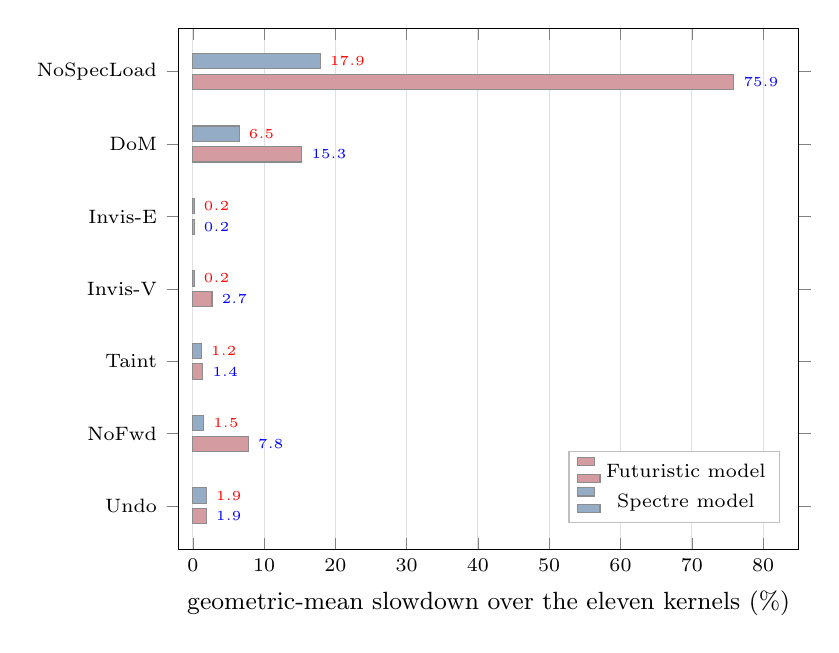
\begin{tikzpicture}
\begin{axis}[xbar, width=0.78\linewidth, height=8.2cm, bar width=5.5pt,
  xmin=-2, xmax=85, enlarge y limits=0.10,
  symbolic y coords={Undo,NoFwd,Taint,Invis-V,Invis-E,DoM,NoSpecLoad}, ytick=data,
  yticklabel style={font=\scriptsize}, xticklabel style={font=\scriptsize},
  xlabel={geometric-mean slowdown over the eleven kernels (\%)}, label style={font=\small},
  nodes near coords, nodes near coords style={font=\tiny},
  every node near coord/.append style={/pgf/number format/fixed, /pgf/number format/precision=1},
  legend style={font=\scriptsize, draw=black!25, at={(0.97,0.05)}, anchor=south east},
  xmajorgrids, grid style={draw=black!12}]
\addplot+[fill=attack!45, draw=black!45] coordinates {(1.9,Undo) (7.8,NoFwd) (1.4,Taint) (2.7,Invis-V) (0.2,Invis-E) (15.3,DoM) (75.9,NoSpecLoad)};
\addlegendentry{Futuristic model}
\addplot+[fill=accent!45, draw=black!45] coordinates {(1.9,Undo) (1.5,NoFwd) (1.2,Taint) (0.2,Invis-V) (0.2,Invis-E) (6.5,DoM) (17.9,NoSpecLoad)};
\addlegendentry{Spectre model}
\end{axis}
\end{tikzpicture}
%% END GENERATED fig_overheads
\caption[Cost of the speculation defences in the model]{Geometric-mean slowdown
of the seven modelled speculation defences over the eleven kernels, under the
Spectre model (a load is safe when all older branches have resolved) and the
Futuristic model (a load is safe when all older instructions have completed).
Results of the model of \Cref{ch:study}, not of hardware.}
\label{fig:overheads}
\end{figure}

\begin{table}[t]
\centering
\caption[Slowdown of each speculation defence per kernel]{Slowdown in per cent
of each modelled speculation defence, Spectre model, against the undefended
model. A negative value is a speedup. The Futuristic table is in
\Cref{app:results}.}
\label{tab:defcost}
\footnotesize
%% BEGIN GENERATED tab_defcost_spectre
\begin{tabular}{@{}lrrrrrrr@{}}
\toprule
\textbf{Kernel} & \textbf{NoSpecLoad} & \textbf{DoM} & \textbf{Invis-E} & \textbf{Invis-V} & \textbf{Taint} & \textbf{NoFwd} & \textbf{Undo} \\
\midrule
\texttt{matmul} & 0.0 & 0.0 & 0.0 & 0.0 & 0.0 & 0.0 & 0.0 \\
\texttt{heapsort} & 17.2 & 0.7 & $-$0.3 & $-$0.3 & 0.2 & 0.3 & $-$0.2 \\
\texttt{listwalk} & 1.8 & 1.8 & 0.0 & 0.0 & 0.0 & 0.0 & 0.0 \\
\texttt{bsearch} & 41.8 & 37.3 & $-$3.5 & $-$3.5 & 5.6 & 6.3 & 6.9 \\
\texttt{bstree} & 24.6 & 1.9 & 0.0 & 0.0 & 3.1 & 4.0 & 0.0 \\
\texttt{crc32} & 0.0 & 0.0 & 0.0 & 0.0 & 0.0 & 0.0 & 0.0 \\
\texttt{sieve} & 56.0 & 0.8 & 0.4 & 0.4 & 0.0 & 0.7 & 0.4 \\
\texttt{hashtab} & 55.1 & 38.7 & 5.8 & 6.1 & 4.8 & 5.9 & 14.9 \\
\texttt{stream} & 0.0 & 0.0 & 0.0 & 0.0 & 0.0 & 0.0 & 0.0 \\
\texttt{fibcall} & 4.7 & 0.0 & 0.0 & 0.0 & 0.0 & 0.0 & 0.0 \\
\texttt{strsearch} & 14.3 & 0.2 & 0.1 & 0.1 & 0.0 & 0.1 & 0.1 \\
\midrule
\textbf{geometric mean} & \textbf{17.9} & \textbf{6.5} & \textbf{0.2} & \textbf{0.2} & \textbf{1.2} & \textbf{1.5} & \textbf{1.9} \\
worst kernel & 56.0 & 38.7 & 5.8 & 6.1 & 5.6 & 6.3 & 14.9 \\
\bottomrule
\end{tabular}
%% END GENERATED tab_defcost_spectre
\end{table}

\begin{finding}
Under the Spectre model, delaying every speculative load costs
\R{geo.spectre.nospec}\pc{} in the geometric mean and up to
\R{worst.spectre.nospec}\pc{} on one kernel. Delaying only the loads that miss
costs \R{geo.spectre.dom}\pc{} (worst \R{worst.spectre.dom}\pc{}); tracking
taint costs \R{geo.spectre.stt}\pc{} (worst \R{worst.spectre.stt}\pc{}),
withholding results \R{geo.spectre.nda}\pc{}, and undoing transient fills
\R{geo.spectre.undo}\pc{}. Under the Futuristic model the same mechanisms cost
\R{geo.futuristic.nospec}\pc{}, \R{geo.futuristic.dom}\pc{},
\R{geo.futuristic.stt}\pc{}, \R{geo.futuristic.nda}\pc{} and
\R{geo.futuristic.undo}\pc{}.
\end{finding}

Three features of \Cref{tab:defcost} deserve comment.

\textbf{The mean hides the distribution.} Three of the eleven kernels pay
nothing for any defence, and two more pay only for the most restrictive one,
because their branches resolve before their loads could have issued anyway. The cost is concentrated in the kernels whose
branches depend on loaded data: \code{bsearch}, \code{hashtab}, \code{bstree}
and \code{heapsort}. A suite with more such programs would report a higher
mean for the same mechanism.

\textbf{Hiding can be a speedup.} For \code{bsearch} the invisible-load
schemes are \R{speedup.spectre.invis-e.bsearch}\pc{} \emph{faster} than no
defence. Its wrong paths issue loads into the wrong half of the table, and in
the undefended model those loads evict useful lines from the first-level
cache. For \code{hashtab} the same schemes cost
\R{slow.spectre.invis-e.hashtab}\pc{}, because there the wrong-path loads were
acting as prefetches. Both effects are known from the study of wrong-path
references~\citep{mutlu2005analysis}.

\textbf{The modelled costs are lower than the published ones} for the schemes
that have a published counterpart. The kernels are small, the model has no
limit on execution ports or queue entries, and its invisible-load scheme omits
the validation squashes and the buffer management of a real design. The model
supports statements about ordering and shape. It does not reproduce the
magnitudes of \Cref{tab:reported}.

\section{What each defence leaves behind}
\label{sec:footprint}

Cost is half of the comparison. \Cref{tab:footprint} gives the other half: the
transient activity that remains under each mechanism, summed over all kernels.

\begin{table}[t]
\centering
\caption[Transient footprint under each defence]{Transient activity under each
modelled defence, Spectre model, summed over the eleven kernels. The first four
rows are what remains for an observer to find; the last three are the work the
defence does.}
\label{tab:footprint}
\scriptsize
%% BEGIN GENERATED tab_footprint
\begin{tabularx}{\linewidth}{@{}Xrrrrrrrr@{}}
\toprule
\textbf{Summed over all kernels} & \textbf{none} & \textbf{NoSpecLoad} & \textbf{DoM} & \textbf{Invis-E} & \textbf{Invis-V} & \textbf{Taint} & \textbf{NoFwd} & \textbf{Undo} \\
\midrule
Transient loads executed & 2\,527\,122 & 0 & 1\,802\,038 & 2\,522\,459 & 2\,522\,031 & 2\,676\,792 & 2\,697\,476 & 2\,522\,493 \\
First-level fills left behind & 527\,708 & 0 & 0 & 0 & 0 & 538\,159 & 543\,661 & 0 \\
Dependent transient loads executed & 7\,221 & 0 & 6\,458 & 7\,101 & 7\,101 & 0 & 0 & 7\,101 \\
Dependent fills left behind & 133 & 0 & 0 & 0 & 0 & 0 & 0 & 0 \\
Fills hidden or rolled back & 0 & 0 & 0 & 832\,839 & 832\,450 & 0 & 0 & 832\,869 \\
Committed loads delayed & 0 & 2\,780\,416 & 410\,878 & 0 & 0 & 393\,453 & 0 & 0 \\
Second (exposure) accesses & 0 & 0 & 0 & 2\,734\,213 & 2\,732\,227 & 0 & 0 & 0 \\
\bottomrule
\end{tabularx}
%% END GENERATED tab_footprint
\end{table}

The table separates the mechanisms into the two groups of \Cref{sec:coverage}.
NoSpecLoad, DoM, the invisible schemes and Undo leave no transient fill in the
first-level cache; of these, only NoSpecLoad also prevents dependent transient
loads from executing. Taint and NoFwd execute no dependent transient load at
all, and leave the independent transient fills in place:
\R{foot.pct.stt}\pc{} and \R{foot.pct.nda}\pc{} of the undefended count, slightly
more than without a defence because the delays they introduce lengthen some
windows. \Cref{fig:pareto} plots the two dimensions against each other.

\begin{figure}[t]
\centering
%% BEGIN GENERATED fig_pareto
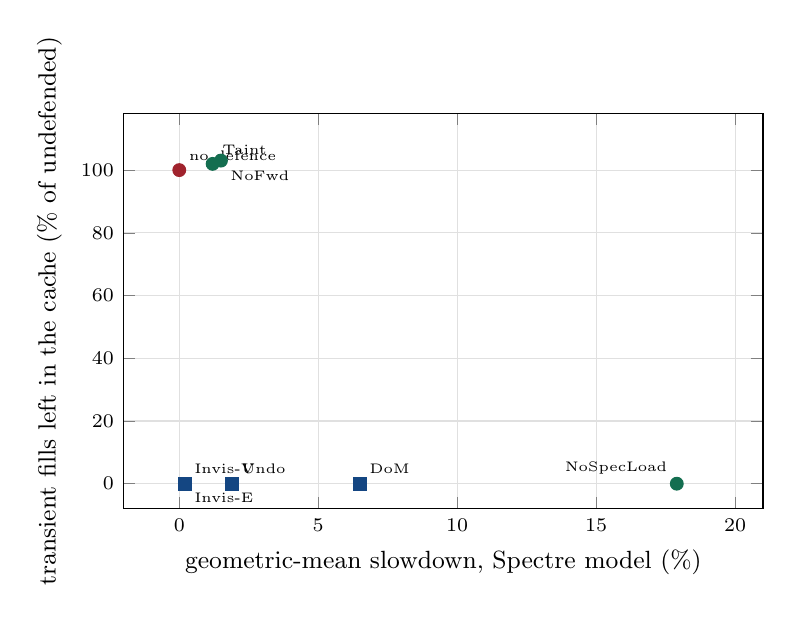
\begin{tikzpicture}
\begin{axis}[width=0.80\linewidth, height=6.6cm,
  xlabel={geometric-mean slowdown, Spectre model (\%)},
  ylabel={transient fills left in the cache (\% of undefended)},
  xmin=-2, xmax=21, ymin=-8, ymax=118, tick label style={font=\scriptsize},
  label style={font=\small}, xmajorgrids, ymajorgrids, grid style={draw=black!12}]
\addplot[only marks, mark=*, mark size=2.3pt, draw=attack, fill=attack] coordinates {(0.00,100.00)};
\node[font=\tiny, anchor=south west] at (axis cs:0.00,100.00) {no defence};
\addplot[only marks, mark=*, mark size=2.3pt, draw=defense, fill=defense] coordinates {(17.90,0.00)};
\node[font=\tiny, anchor=south east] at (axis cs:17.90,0.00) {NoSpecLoad};
\addplot[only marks, mark=square*, mark size=2.3pt, draw=accent, fill=accent] coordinates {(6.50,0.00)};
\node[font=\tiny, anchor=south west] at (axis cs:6.50,0.00) {DoM};
\addplot[only marks, mark=square*, mark size=2.3pt, draw=accent, fill=accent] coordinates {(0.20,0.00)};
\node[font=\tiny, anchor=north west] at (axis cs:0.20,0.00) {Invis-E};
\addplot[only marks, mark=square*, mark size=2.3pt, draw=accent, fill=accent] coordinates {(0.20,0.00)};
\node[font=\tiny, anchor=south west] at (axis cs:0.20,0.00) {Invis-V};
\addplot[only marks, mark=*, mark size=2.3pt, draw=defense, fill=defense] coordinates {(1.20,101.98)};
\node[font=\tiny, anchor=south west] at (axis cs:1.20,101.98) {Taint};
\addplot[only marks, mark=*, mark size=2.3pt, draw=defense, fill=defense] coordinates {(1.50,103.02)};
\node[font=\tiny, anchor=north west] at (axis cs:1.50,103.02) {NoFwd};
\addplot[only marks, mark=square*, mark size=2.3pt, draw=accent, fill=accent] coordinates {(1.90,0.00)};
\node[font=\tiny, anchor=south west] at (axis cs:1.90,0.00) {Undo};
\end{axis}
\end{tikzpicture}
%% END GENERATED fig_pareto
\caption[Cost against residual transient footprint]{Cost against what remains,
for the modelled defences under the Spectre model. Horizontal: geometric-mean
slowdown. Vertical: first-level fills left by transient loads, as a share of
the undefended count. The red marker is the undefended model. Round green
markers execute no dependent transient load; square blue markers do. No
mechanism is at the origin with a round marker.}
\label{fig:pareto}
\end{figure}

No point of \Cref{fig:pareto} dominates. The mechanisms near the origin hide
the fills but still run the dependent loads; the ones that stop the dependent
loads cheaply leave the fills; the one that does both costs an order of
magnitude more. A comparison on one axis alone would have picked a winner that
the other axis disqualifies.

\section{The baseline moves the cost}
\label{sec:sensitivity}

\Cref{tab:sensitivity} repeats the measurement while one parameter of the
baseline core is varied, and \Cref{fig:sens} plots two of the sweeps.

\begin{table}[t]
\centering
\caption[Defence cost against the baseline configuration]{Geometric-mean
slowdown in per cent of each modelled defence (Spectre model) when the
baseline core is varied in pipeline width, reorder-buffer size or first-level
cache latency. The second column is the geometric-mean IPC of the undefended
baseline.}
\label{tab:sensitivity}
\footnotesize
%% BEGIN GENERATED tab_sensitivity
\begin{tabular}{@{}lrrrrrrrr@{}}
\toprule
\textbf{Baseline} & \textbf{IPC} & \textbf{NoSpecLoad} & \textbf{DoM} & \textbf{Invis-E} & \textbf{Invis-V} & \textbf{Taint} & \textbf{NoFwd} & \textbf{Undo} \\
\midrule
Width = 2 & 0.937 & 11.0 & 5.5 & 0.1 & 0.1 & 1.1 & 1.3 & 1.2 \\
Width = 4 & 1.160 & 17.9 & 6.5 & 0.2 & 0.2 & 1.2 & 1.5 & 1.9 \\
Width = 8 & 1.300 & 22.2 & 7.2 & 0.5 & 0.5 & 1.3 & 1.7 & 2.4 \\
\midrule
ROB entries = 32 & 1.048 & 15.7 & 4.9 & 0.1 & 0.6 & 0.7 & 0.9 & 0.9 \\
ROB entries = 64 & 1.109 & 17.2 & 6.0 & 0.1 & 0.3 & 1.1 & 1.4 & 1.5 \\
ROB entries = 128 & 1.160 & 17.9 & 6.5 & 0.2 & 0.2 & 1.2 & 1.5 & 1.9 \\
ROB entries = 256 & 1.180 & 18.1 & 6.8 & 0.3 & 0.3 & 1.3 & 1.6 & 2.1 \\
\midrule
L1 latency = 2 & 1.248 & 11.3 & 6.3 & 0.2 & 0.2 & 1.2 & 1.6 & 1.7 \\
L1 latency = 4 & 1.160 & 17.9 & 6.5 & 0.2 & 0.2 & 1.2 & 1.5 & 1.9 \\
L1 latency = 6 & 1.089 & 25.2 & 6.8 & 0.3 & 0.3 & 1.3 & 1.5 & 2.2 \\
\bottomrule
\end{tabular}
%% END GENERATED tab_sensitivity
\end{table}

\begin{figure}[t]
\centering
%% BEGIN GENERATED fig_sens
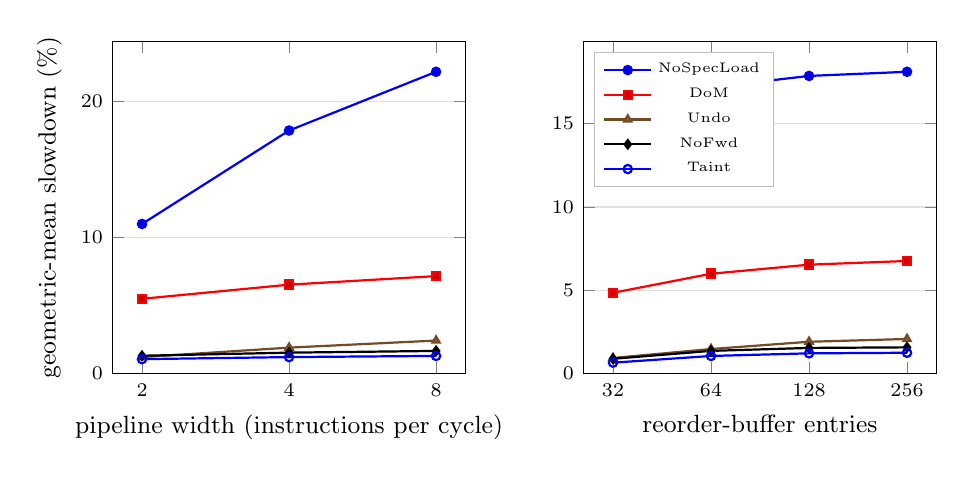
\begin{tikzpicture}
\begin{groupplot}[group style={group size=2 by 1, horizontal sep=1.5cm},
  width=0.50\linewidth, height=5.8cm, tick label style={font=\scriptsize},
  label style={font=\small}, ymajorgrids, grid style={draw=black!12}, ymin=0,
  legend style={font=\tiny, draw=black!25}]
\nextgroupplot[xmode=log, log basis x=2, xtick={2,4,8}, xticklabels={2,4,8}, ylabel={geometric-mean slowdown (\%)}, xlabel={pipeline width (instructions per cycle)}]
\addplot+[mark=*, mark size=1.5pt, thick] coordinates {(2,11.002) (4,17.865) (8,22.178)};
\addplot+[mark=square*, mark size=1.5pt, thick] coordinates {(2,5.503) (4,6.543) (8,7.171)};
\addplot+[mark=triangle*, mark size=1.5pt, thick] coordinates {(2,1.225) (4,1.918) (8,2.437)};
\addplot+[mark=diamond*, mark size=1.5pt, thick] coordinates {(2,1.322) (4,1.549) (8,1.676)};
\addplot+[mark=o, mark size=1.5pt, thick] coordinates {(2,1.072) (4,1.224) (8,1.309)};
\nextgroupplot[xmode=log, log basis x=2, xtick={32,64,128,256}, xticklabels={32,64,128,256}, legend pos=north west, xlabel={reorder-buffer entries}]
\addplot+[mark=*, mark size=1.5pt, thick] coordinates {(32,15.689) (64,17.183) (128,17.865) (256,18.114)};
\addlegendentry{NoSpecLoad}
\addplot+[mark=square*, mark size=1.5pt, thick] coordinates {(32,4.855) (64,5.999) (128,6.543) (256,6.765)};
\addlegendentry{DoM}
\addplot+[mark=triangle*, mark size=1.5pt, thick] coordinates {(32,0.945) (64,1.484) (128,1.918) (256,2.086)};
\addlegendentry{Undo}
\addplot+[mark=diamond*, mark size=1.5pt, thick] coordinates {(32,0.896) (64,1.372) (128,1.549) (256,1.584)};
\addlegendentry{NoFwd}
\addplot+[mark=o, mark size=1.5pt, thick] coordinates {(32,0.664) (64,1.067) (128,1.224) (256,1.259)};
\addlegendentry{Taint}
\end{groupplot}
\end{tikzpicture}
%% END GENERATED fig_sens
\caption[Defence cost against pipeline width and window size]{Geometric-mean
slowdown of five modelled defences against the width of the pipeline (left)
and the size of the reorder buffer (right). Every curve rises: the same
mechanism costs more on a more aggressive core.}
\label{fig:sens}
\end{figure}

\begin{finding}
Going from a two-wide to an eight-wide core raises the cost of delaying all
speculative loads from \R{sens.width.2.nospec}\pc{} to
\R{sens.width.8.nospec}\pc{}, of delay-on-miss from \R{sens.width.2.dom}\pc{} to
\R{sens.width.8.dom}\pc{}, and of undo from \R{sens.width.2.undo}\pc{} to
\R{sens.width.8.undo}\pc{}. Growing the reorder buffer from 32 to 256 entries
raises delay-on-miss from \R{sens.rob.32.dom}\pc{} to \R{sens.rob.256.dom}\pc{}.
The first reason of \Cref{sec:incomparable} is therefore not a caveat but a
measurable effect of a factor of two within one model.
\end{finding}

\section{Isolation between domains}
\label{sec:isocost}

For the isolation mechanisms the experiment of \Cref{sec:interference} is
repeated with timing: two kernels alternate on one core, and the time for both
to finish is compared with the unprotected run. \Cref{tab:isolation} gives the
result for a time slice of \num{100000} instructions.

\begin{table}[t]
\centering
\caption[Cost of isolation mechanisms]{Slowdown in per cent of five isolation
mechanisms in the model for five pairs of kernels sharing one core, with a context switch
every \num{100000} instructions. Each entry is the mean over five page-frame
layouts, with the smallest and largest value in parentheses.}
\label{tab:isolation}
\scriptsize\setlength{\tabcolsep}{3.5pt}%
%% BEGIN GENERATED tab_isolation
\begin{tabular}{@{}lrrrrr@{}}
\toprule
\textbf{Pair of kernels} & \textbf{Flush} & \textbf{Flush+Colour} & \textbf{Colour} & \textbf{WayPart} & \textbf{RandLLC} \\
\midrule
\texttt{crc32 + hashtab} & 2.9 {\tiny(2.9 to 3.0)} & 12.9 {\tiny(12.1 to 13.5)} & 9.0 {\tiny(8.2 to 9.6)} & 16.1 {\tiny(15.3 to 16.8)} & 0.3 {\tiny(0.3 to 0.4)} \\
\texttt{bsearch + stream} & 0.5 {\tiny(0.4 to 0.5)} & 17.9 {\tiny(11.7 to 25.6)} & 17.5 {\tiny(11.3 to 25.1)} & 24.6 {\tiny(19.5 to 30.0)} & 4.9 {\tiny(0.0 to 10.4)} \\
\texttt{heapsort + matmul} & 1.1 {\tiny(1.1 to 1.1)} & 2.2 {\tiny(2.0 to 2.4)} & 1.2 {\tiny(1.0 to 1.4)} & 5.2 {\tiny(4.7 to 5.5)} & 0.0 {\tiny(0.0 to 0.0)} \\
\texttt{listwalk + sieve} & 0.1 {\tiny(0.1 to 0.1)} & 117.9 {\tiny(94.7 to 144.4)} & 117.7 {\tiny(94.2 to 144.2)} & 125.2 {\tiny(102.3 to 151.2)} & 4.3 {\tiny($-$6.3 to 10.5)} \\
\texttt{bstree + strsearch} & 0.8 {\tiny(0.7 to 0.8)} & 12.0 {\tiny(10.9 to 14.1)} & 11.1 {\tiny(10.0 to 13.0)} & 28.2 {\tiny(27.1 to 31.2)} & 0.2 {\tiny(0.2 to 0.3)} \\
\midrule
\textbf{geometric mean} & \textbf{1.1} & \textbf{27.1} & \textbf{25.7} & \textbf{34.4} & \textbf{1.9} \\
\bottomrule
\end{tabular}
%% END GENERATED tab_isolation
\end{table}

\begin{figure}[t]
\centering
%% BEGIN GENERATED fig_flushq
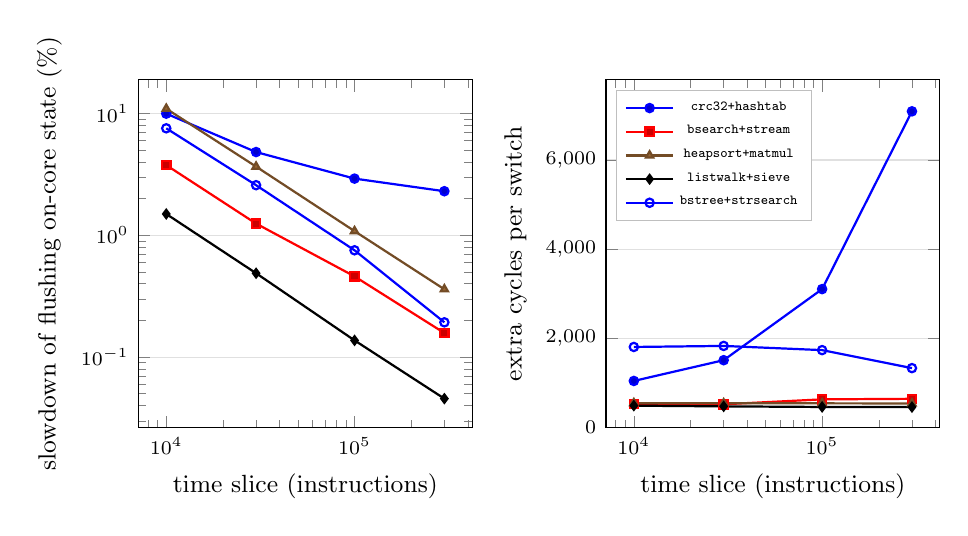
\begin{tikzpicture}
\begin{groupplot}[group style={group size=2 by 1, horizontal sep=1.7cm},
  width=0.48\linewidth, height=6.0cm, xmode=log, tick label style={font=\scriptsize},
  xlabel={time slice (instructions)}, label style={font=\small},
  ymajorgrids, grid style={draw=black!12}, legend style={font=\tiny, draw=black!25}]
\nextgroupplot[ymode=log, ylabel={slowdown of flushing on-core state (\%)}]
\addplot+[mark=*, mark size=1.5pt, thick] coordinates {(10000,9.9738) (30000,4.8258) (100000,2.9214) (300000,2.3014)};
\addplot+[mark=square*, mark size=1.5pt, thick] coordinates {(10000,3.7702) (30000,1.2482) (100000,0.4600) (300000,0.1576)};
\addplot+[mark=triangle*, mark size=1.5pt, thick] coordinates {(10000,10.9542) (30000,3.6662) (100000,1.0824) (300000,0.3604)};
\addplot+[mark=diamond*, mark size=1.5pt, thick] coordinates {(10000,1.4974) (30000,0.4882) (100000,0.1372) (300000,0.0456)};
\addplot+[mark=o, mark size=1.5pt, thick] coordinates {(10000,7.5628) (30000,2.5798) (100000,0.7534) (300000,0.1930)};
\nextgroupplot[ylabel={extra cycles per switch}, ymin=0, legend pos=north west]
\addplot+[mark=*, mark size=1.5pt, thick] coordinates {(10000,1046.5) (30000,1511.8) (100000,3105.3) (300000,7089.8)};
\addlegendentry{\texttt{crc32+hashtab}}
\addplot+[mark=square*, mark size=1.5pt, thick] coordinates {(10000,529.6) (30000,523.3) (100000,633.8) (300000,645.9)};
\addlegendentry{\texttt{bsearch+stream}}
\addplot+[mark=triangle*, mark size=1.5pt, thick] coordinates {(10000,549.1) (30000,545.4) (100000,544.5) (300000,541.9)};
\addlegendentry{\texttt{heapsort+matmul}}
\addplot+[mark=diamond*, mark size=1.5pt, thick] coordinates {(10000,492.3) (30000,476.6) (100000,463.3) (300000,460.8)};
\addlegendentry{\texttt{listwalk+sieve}}
\addplot+[mark=o, mark size=1.5pt, thick] coordinates {(10000,1808.2) (30000,1831.4) (100000,1737.3) (300000,1334.0)};
\addlegendentry{\texttt{bstree+strsearch}}
\end{groupplot}
\end{tikzpicture}
%% END GENERATED fig_flushq
\caption[Cost of flushing against the time slice]{Flushing the on-core state at
every context switch, in the model. Left: slowdown against the length of the time slice, both
axes logarithmic; the slowdown falls as the slice grows. Right: the additional
cycles per switch, which include the 322 cycles charged for the flush itself
and the refill that follows; they rise with the slice until the flushed
structures are full again.}
\label{fig:flushq}
\end{figure}

\textbf{Flushing costs per switch.} \Cref{fig:flushq} shows that the cost of
flushing the first-level caches, the TLB and the predictors is a bounded number
of cycles per switch, between \R{flush.perswitch.min} and
\R{flush.perswitch.max} in these runs. It grows with the amount of state the
incoming domain touches again during its slice and saturates once the flushed
structures are full, so the relative slowdown falls as the time slice grows. Scaled to a slice of $10^7$ cycles the same per-switch cost
would be between \R{flush.extrap.min}\pc{} and \R{flush.extrap.max}\pc{}. This
is below the 0.7\pc{} measured on CVA6~\citep{wistoff2023systematic}, as it
should be: the kernels here refill a few hundred lines, real applications
considerably more.

\textbf{Partitioning costs capacity.} Colouring and way partitioning cost the
same at every slice length (\Cref{app:results}), because what they take away is
capacity, not warm state. How much that costs is decided by the pair: between
\R{iso.WayPart.heapsort+matmul}\pc{} for two kernels that fit in half of each
cache and \R{iso.WayPart.listwalk+sieve}\pc{} for a pair in which one kernel no
longer fits. This is the cliff of \Cref{fig:llcsweep} seen from the other side.
The spread over page-frame layouts is itself large for the pairs near the
cliff, which is the page-placement effect of Kessler and
Hill~\citep{kessler1992page}.

\textbf{A randomised index costs latency.} Encrypting the last-level index adds
two cycles to every access that reaches that level and leaves capacity alone.
For single kernels the geometric-mean cost is \R{rand.1600.geo}\pc{} and the
worst \R{rand.1600.worst}\pc{} at the remapping rate that corresponds to
CEASER's default; remapping sixteen times as often raises the worst case to
\R{rand.100.worst}\pc{} (\Cref{app:results}).

\begin{finding}
In this model the cost of isolation is governed less by the mechanism than by
the distance between the working sets and the capacity that remains. Flushing
is cheap whenever time slices are long; partitioning is cheap whenever the
working sets are small; neither is cheap for a workload that switches often
\emph{and} fills the cache. A single average over pairs,
\R{iso.Flush.geo}\pc{} for flushing against \R{iso.WayPart.geo}\pc{} for way
partitioning here, conceals exactly the cases a system designer has to plan
for.
\end{finding}

\section{Memory traffic and energy}
\label{sec:traffic}

Cycles are not the only cost. \Cref{tab:traffic} shows how each speculation
defence changes the number of accesses at each level of the hierarchy,
including the accesses that hiding schemes make out of sight.

\begin{table}[t]
\centering
\caption[Memory-hierarchy traffic under each defence]{Change in the number of
accesses at each level of the hierarchy and in total cycles, summed over the
eleven kernels, relative to the undefended model (per cent, Spectre model).
Invisible and rolled-back accesses are counted at the levels they reach.}
\label{tab:traffic}
\footnotesize
%% BEGIN GENERATED tab_traffic
\begin{tabular}{@{}lrrrrr@{}}
\toprule
\textbf{Defence} & \textbf{L1 accesses} & \textbf{L2 accesses} & \textbf{LLC accesses} & \textbf{Memory accesses} & \textbf{Total cycles} \\
\midrule
NoSpecLoad & $-$27.8 & $-$40.1 & $-$33.2 & $-$4.4 & +23.6 \\
DoM & $-$10.0 & $-$40.1 & $-$33.2 & $-$4.4 & +11.5 \\
Invis-E & +24.7 & +50.7 & +63.9 & +29.0 & +0.2 \\
Invis-V & +24.7 & +50.7 & +63.9 & +29.0 & +0.2 \\
Taint & +1.5 & +0.6 & +0.4 & +0.1 & +2.3 \\
NoFwd & +1.7 & +0.9 & +0.5 & +0.3 & +2.9 \\
Undo & $-$2.7 & +20.5 & +31.7 & +29.0 & +2.9 \\
\bottomrule
\end{tabular}
%% END GENERATED tab_traffic
\end{table}

The mechanisms that stop transient loads reduce traffic, since the loads never
reach the outer levels. The invisible schemes increase it at every level:
each speculative load is made visible by a second access, and a transient load
that is hidden leaves nothing behind for the next one to hit, so the same line
is fetched again. Memory accesses rise by
$\R{traffic.invis-e.memory_accesses}$\pc{} for a scheme whose cost in cycles is
close to zero.

This matters for energy, which the model does not measure. What can be said
without a power model is a bound. If a defence leaves the energy of a run
unchanged, the energy-delay product grows in proportion to the run time; if it
leaves the average power unchanged, it grows with the square
(\Cref{app:metrics}). A defence with a slowdown $S$ therefore raises the
energy-delay product by between $S$ and $2S + S^2$, and \Cref{tab:traffic}
indicates on which side of that range a mechanism falls: one that adds memory
traffic adds energy as well as time. The only published energy figures in
\Cref{tab:reported}, those for delay-on-miss, are consistent with this
reading.\index{energy-delay product (EDP)}

\section{Storage}
\label{sec:storage}

\Cref{tab:area} accounts for the state that each modelled mechanism needs in
the configuration of the study. The figures are arithmetic on the parameters
of the model. They are not synthesis results and say nothing about logic or
timing; where the authors of a design report storage, their figure is given
for comparison.

\begin{table}[t]
\centering
\caption[Storage implied by each modelled mechanism]{State required by each
mechanism as modelled, for the study configuration: 8-way first- and
second-level caches, a 16-way last level of 2\,MiB, a 128-entry reorder buffer
and, for the per-load entries, the 32-entry load queue of the published
baselines. The author's accounting, not a synthesis result.}
\label{tab:area}
\footnotesize
\begin{tabularx}{\linewidth}{@{}>{\raggedright\arraybackslash}p{2.6cm}X>{\raggedright\arraybackslash}p{2.1cm}@{}}
\toprule
\textbf{Mechanism} & \textbf{State and how it is counted} & \textbf{Bits} \\
\midrule
Way partitioning &
A fill mask and a hit mask per domain for each of four caches (8, 8, 8 and 16
ways), two domains; a second history register (12 bits) and return stack
($16 \times 64$ bits). &
$160 + 1036$ \\
Page colouring & None in hardware; a constraint on the page allocator. & 0 \\
Flush at a switch &
A counter that walks the largest structure flushed (4096 pattern-table
entries). & 12 \\
Randomised index &
Two 64-bit keys, an 11-bit set pointer, an 11-bit access counter, and one
key-epoch bit per line ($\num{32768}$ lines). CEASER reports under 24 bytes for
its own bookkeeping. &
$\num{32918}$ \\
Invisible loads &
One line buffer per load-queue entry: 512 data bits, 58 address bits, one valid
bit. & $32 \times 571 = \num{18272}$ \\
Undo &
Per load-queue entry: set and way of the installed line (9 bits), address of
the evicted line (58 bits), one valid bit. CleanupSpec reports under 1\,KB. &
$32 \times 68 = \num{2176}$ \\
Delay-on-miss & One ``delayed'' bit per load-queue entry. & 32 \\
Taint &
Per physical register, the reorder-buffer index of the youngest speculative
access it depends on (7 bits) and a valid bit; 160 physical registers. &
$160 \times 8 = \num{1280}$ \\
No forwarding & One ``unsafe'' bit per reorder-buffer entry. & 128 \\
\bottomrule
\end{tabularx}
\end{table}

The largest entry is about 4\,KiB, a fifth of a per cent of the last-level
cache it protects, and most are far smaller. Storage is not where the cost of
these mechanisms lies. It lies in time (\Cref{tab:defcost}), in capacity
(\Cref{tab:isolation}) and in memory traffic (\Cref{tab:traffic}); and, for a
real design, in the logic on timing-critical paths and in verification effort,
neither of which a model of this kind can measure.

\section{Combining defences}
\label{sec:composition}

\Cref{tab:coverage} showed that a system which wants protection both between
domains and within one needs a mechanism from each half of the table. The
literature evaluates mechanisms singly. \Cref{tab:composition} measures five
combinations of an isolation mechanism $A$ with a speculation defence $B$ on
the five pairs of kernels, and compares the slowdown of the combination,
$S_{AB}$, with the product $(1+S_A)(1+S_B)-1$ that independent costs would
give.

\begin{table}[t]
\centering
\caption[Cost of combined defences]{Slowdown in per cent, in the model, of an
isolation mechanism $A$, a speculation defence $B$, and both together, for pairs of
kernels switching every \num{100000} instructions. \emph{Product} is
$(1+S_A)(1+S_B)-1$; \emph{Excess} is $S_{AB}$ minus the product, in percentage
points.}
\label{tab:composition}
\scriptsize
%% BEGIN GENERATED tab_composition
\begin{tabular}{@{}lllrrrrr@{}}
\toprule
\textbf{Pair} & \textbf{A} & \textbf{B} & $S_A$ & $S_B$ & $S_{AB}$ & \textbf{Product} & \textbf{Excess} \\
\midrule
\texttt{crc32 + hashtab} & Flush+Colour & Taint & 13.4 & 2.7 & 17.7 & 16.4 & +1.2 \\
\texttt{crc32 + hashtab} & Flush+Colour & DoM & 13.4 & 27.4 & 48.0 & 44.5 & +3.5 \\
\texttt{crc32 + hashtab} & WayPart & Taint & 16.6 & 2.7 & 20.0 & 19.7 & +0.3 \\
\texttt{crc32 + hashtab} & WayPart & Invis-V & 16.6 & 6.4 & 26.5 & 24.0 & +2.5 \\
\texttt{crc32 + hashtab} & RandLLC & NoFwd & 0.3 & 3.3 & 3.7 & 3.6 & +0.1 \\
\midrule
\texttt{bsearch + stream} & Flush+Colour & Taint & 11.7 & 4.1 & 15.6 & 16.3 & $-$0.7 \\
\texttt{bsearch + stream} & Flush+Colour & DoM & 11.7 & 34.5 & 44.1 & 50.2 & $-$6.2 \\
\texttt{bsearch + stream} & WayPart & Taint & 19.5 & 4.1 & 24.6 & 24.4 & +0.2 \\
\texttt{bsearch + stream} & WayPart & Invis-V & 19.5 & 1.7 & 15.0 & 21.5 & $-$6.5 \\
\texttt{bsearch + stream} & RandLLC & NoFwd & 0.0 & 4.6 & 4.8 & 4.5 & +0.3 \\
\midrule
\texttt{heapsort + matmul} & Flush+Colour & Taint & 2.1 & 0.2 & 3.1 & 2.3 & +0.7 \\
\texttt{heapsort + matmul} & Flush+Colour & DoM & 2.1 & 1.1 & 2.8 & 3.2 & $-$0.4 \\
\texttt{heapsort + matmul} & WayPart & Taint & 4.7 & 0.2 & 5.6 & 4.9 & +0.7 \\
\texttt{heapsort + matmul} & WayPart & Invis-V & 4.7 & 0.1 & 3.3 & 4.8 & $-$1.5 \\
\texttt{heapsort + matmul} & RandLLC & NoFwd & 0.0 & 0.3 & 0.3 & 0.3 & +0.0 \\
\midrule
\texttt{listwalk + sieve} & Flush+Colour & Taint & 94.7 & 0.0 & 94.7 & 94.7 & 0.0 \\
\texttt{listwalk + sieve} & Flush+Colour & DoM & 94.7 & 1.5 & 95.8 & 97.6 & $-$1.8 \\
\texttt{listwalk + sieve} & WayPart & Taint & 122.0 & 0.0 & 122.0 & 122.0 & 0.0 \\
\texttt{listwalk + sieve} & WayPart & Invis-V & 122.0 & 0.0 & 122.1 & 122.1 & +0.1 \\
\texttt{listwalk + sieve} & RandLLC & NoFwd & 5.8 & 0.1 & 5.8 & 5.8 & 0.0 \\
\midrule
\texttt{bstree + strsearch} & Flush+Colour & Taint & 11.8 & 2.6 & 14.4 & 14.7 & $-$0.3 \\
\texttt{bstree + strsearch} & Flush+Colour & DoM & 11.8 & 1.6 & 13.4 & 13.6 & $-$0.2 \\
\texttt{bstree + strsearch} & WayPart & Taint & 27.6 & 2.6 & 29.5 & 30.9 & $-$1.4 \\
\texttt{bstree + strsearch} & WayPart & Invis-V & 27.6 & 0.0 & 26.7 & 27.6 & $-$0.9 \\
\texttt{bstree + strsearch} & RandLLC & NoFwd & 0.2 & 3.5 & 3.7 & 3.7 & 0.0 \\
\bottomrule
\end{tabular}
%% END GENERATED tab_composition
\end{table}

\begin{finding}
In \R{comp.within1} of the \R{comp.n} combinations the measured slowdown is
within one percentage point of the product of the individual slowdowns, and
the largest deviations are $\R{comp.max}$ and $\R{comp.min}$ points. To first
order the costs multiply. The deviations have a common cause: an isolation
mechanism changes the miss rate, and the cost of a speculation defence depends
on how long loads take. Where partitioning turns hits into misses,
delay-on-miss has more loads to delay and the combination costs more than the
product; where a hiding scheme removes wrong-path pollution, the smaller
partition suffers less from it and the combination costs less.
\end{finding}

\begin{takeaway}
No mechanism dominates on cost and coverage together, the cost of each depends
on the baseline and on the workload, and the costs of combined mechanisms
multiply. A design therefore composes several, and the question to ask of a
proposed defence is not what it costs on average but which programs pay, and
what it leaves for the next mechanism to cover.
\end{takeaway}


\chapter{The Model Study: Instrument, Validation and Limits}
\label{ch:study}

\section{Purpose and design}

The model study exists to answer one question that the literature cannot:\index{model study!design}
what do representative defences cost, and what do they leave, when everything
except the defence is held constant? Four decisions follow from that purpose.

\begin{itemize}
  \item \textbf{One baseline.} All mechanisms are switches on one simulator,
        so the core, the caches, the workloads and the reporting are identical
        by construction.
  \item \textbf{Benign programs only.} The kernels are ordinary small
        programs. The study measures how a machine behaves and what a defence
        costs; it contains no attack.
  \item \textbf{Validated before use.} No result was taken from the model
        until its functional output agreed with two independent references and
        its timing agreed with values derived by hand (\Cref{sec:validation}).
  \item \textbf{Reproducible from this file.} The simulator and the kernels
        are listed in full in \Cref{app:source,app:kernels}; every table and
        plot of the study is generated from the result files by a script, and
        every number quoted in the text is inserted by a macro from the same
        files.
\end{itemize}

\section{The instrument}
\label{sec:instrument}

\Cref{fig:model} shows the tool chain. A small assembler turns each kernel
into a memory image. The image is executed twice: by QEMU~\citep{bellard2005qemu},
as an independent reference for the result, and by the simulator
\code{rvmodel}, which was written for this paper.

\begin{figure}[t]
\centering
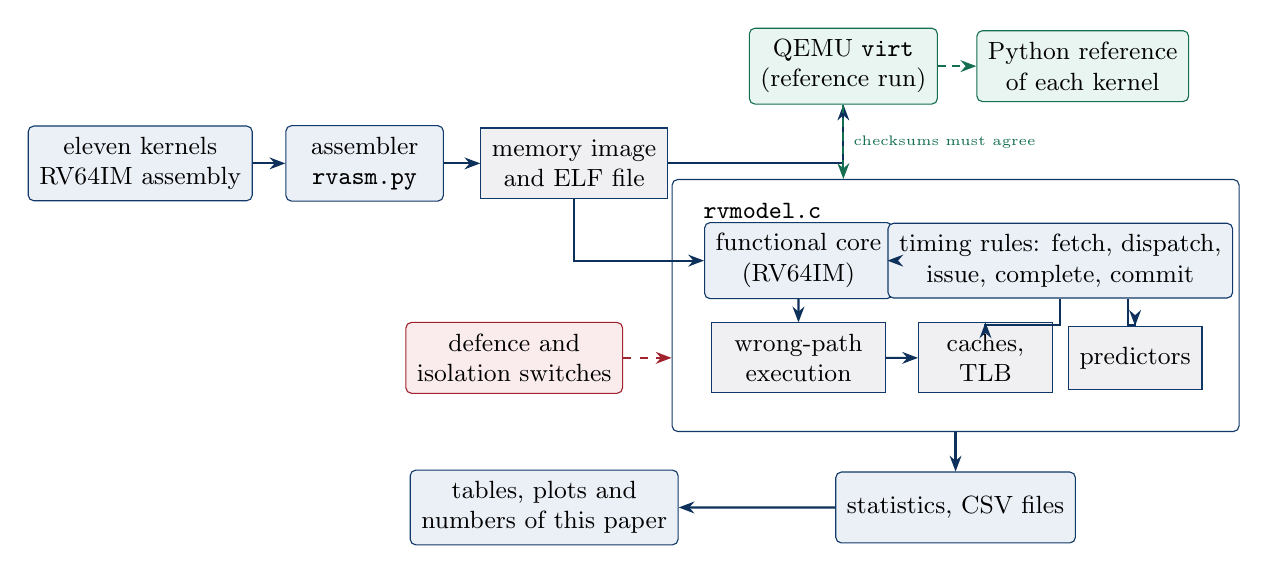
\begin{tikzpicture}[scale=0.95, every node/.style={font=\scriptsize}]
  \node[blk, minimum width=2.3cm, minimum height=0.9cm] (src) at (0,0) {eleven kernels\\RV64IM assembly};
  \node[blk, minimum width=2.0cm, minimum height=0.9cm] (asm) at (3.0,0) {assembler\\\code{rvasm.py}};
  \node[memblk, minimum width=1.9cm, minimum height=0.9cm] (bin) at (5.8,0) {memory image\\and ELF file};
  \node[def, minimum width=2.3cm, minimum height=0.9cm] (qemu) at (9.4,1.3) {QEMU \code{virt}\\(reference run)};
  \node[def, minimum width=2.3cm, minimum height=0.9cm] (ref) at (12.6,1.3) {Python reference\\of each kernel};
  \node[draw=accent!80!black, fill=white, rounded corners=2pt, minimum width=7.2cm,
        minimum height=3.2cm] (sim) at (10.9,-1.9) {};
  \node[font=\scriptsize\bfseries, anchor=north west] at (7.4,-0.4) {\code{rvmodel.c}};
  \node[blk, minimum width=2.2cm, minimum height=0.8cm] (fn) at (8.8,-1.3) {functional core\\(RV64IM)};
  \node[blk, minimum width=3.6cm, minimum height=0.8cm] (tm) at (12.3,-1.3) {timing rules: fetch, dispatch,\\issue, complete, commit};
  \node[memblk, minimum width=2.2cm, minimum height=0.8cm] (wp) at (8.8,-2.6) {wrong-path\\execution};
  \node[memblk, minimum width=1.7cm, minimum height=0.8cm] (ca) at (11.3,-2.6) {caches,\\TLB};
  \node[memblk, minimum width=1.7cm, minimum height=0.8cm] (bp) at (13.3,-2.6) {predictors};
  \node[atk, minimum width=2.4cm, minimum height=0.9cm] (df) at (5.0,-2.6) {defence and\\isolation switches};
  \node[blk, minimum width=2.3cm, minimum height=0.9cm] (csv) at (10.9,-4.6) {statistics, CSV files};
  \node[blk, minimum width=2.6cm, minimum height=0.9cm] (tex) at (5.4,-4.6) {tables, plots and\\numbers of this paper};
  \draw[sig] (src) -- (asm); \draw[sig] (asm) -- (bin);
  \draw[sig] (bin.east) -| (qemu.south);
  \draw[sig] (bin.south) |- (fn.west);
  \draw[sig] (fn) -- (tm); \draw[sig] (fn) -- (wp);
  \draw[sig] (tm.south) -- ++(0,-0.35) -| (ca.north);
  \draw[sig] (tm.south) ++(0.9,0) -- ++(0,-0.35) -| (bp.north);
  \draw[sig] (wp) -- (ca);
  \draw[atksig] (df.east) -- (sim.west |- df.east);
  \draw[sig] (sim.south) -- (csv.north);
  \draw[sig] (csv) -- (tex);
  \draw[defsig, densely dashed] (qemu.east) -- (ref.west);
  \draw[defsig, densely dashed] (qemu.south) -- (qemu.south |- sim.north)
        node[midway, right, font=\tiny, text=defense] {checksums must agree};
\end{tikzpicture}
\caption[Tool chain of the model study]{The tool chain of the model study. One
binary runs on QEMU and on the simulator; the checksum each kernel prints must
agree between QEMU, the simulator and an independent Python implementation of
the kernel. Defences and isolation mechanisms are switches on the timing
rules.}
\label{fig:model}
\end{figure}

The simulator has two layers, mirroring \Cref{ch:proc,ch:pipeline}. The
\emph{functional core} executes RV64IM instructions one at a time, exactly as
the reference machine of \Cref{fig:datapath} would. The \emph{timing layer}
assigns each executed instruction a fetch, dispatch, issue, completion and
commit time from a small set of rules: a fetch and commit width, a reorder
buffer that bounds the instructions in flight, operand readiness, load latency
from the cache and TLB models, and a redirect when a prediction turns out
wrong. This is a first-order model in the sense of Karkhanis and
Smith~\citep{karkhanis2004first}: it captures the window, the dependences and
the miss events, and deliberately not the circuit-level detail of a real core.
After every misprediction the simulator also executes the wrong path, on a
scratch copy of the registers, for as long as the rules say it would run, and
applies its loads to the cache model. \Cref{app:model} states every rule.
\Cref{tab:config} lists the default parameters.

\begin{table}[t]
\centering
\caption[Default configuration of the model]{Default configuration of the
model. Latencies are in cycles from the issue of a load to the availability of
its data.}
\label{tab:config}
\footnotesize
\begin{tabularx}{\linewidth}{@{}>{\raggedright\arraybackslash}p{3.4cm}X@{}}
\toprule
\textbf{Component} & \textbf{Default} \\
\midrule
Pipeline & Fetch, dispatch and commit four instructions per cycle; four cycles
from fetch to dispatch; 128-entry reorder buffer. \\
Execution latencies & One cycle for integer operations, three for
multiplication, twenty for division. \\
Direction predictor & 4096 two-bit counters indexed by the program counter
XORed with twelve bits of global history. \\
Target prediction & 512-entry direct-mapped branch target buffer; 16-entry
return-address stack. \\
First-level caches & Instruction and data, each 32\,KiB, 8 ways, 64-byte
lines, LRU; latency 4. \\
Second-level cache & 256\,KiB, 8 ways; latency 14. \\
Last-level cache & 2\,MiB, 16 ways; latency 45. Memory: latency 220. \\
Data TLB & 32 entries, fully associative, tagged with the domain; a miss
triggers a three-level walk whose loads go through the data caches. \\
Page frames & Assigned pseudo-randomly within each domain; five layouts where a
spread is reported. \\
Context switch & 322 cycles when any structure is flushed, the difference
between the fenced and unfenced switch measured on
CVA6~\citep{wistoff2021fencet}. \\
Randomised index & Two cycles added to last-level latency; one set remapped
every 1600 accesses to that level. \\
\bottomrule
\end{tabularx}
\end{table}

\section{The kernels}
\label{sec:kernels}

The eleven kernels of \Cref{tab:kernels} were written in RISC-V assembly for
this study. They were chosen to cover the behaviours that decide what a
defence costs: working sets from a stack frame to more than a megabyte,
branches from perfectly predictable to essentially random, and load addresses
that do or do not depend on loaded data. Each kernel generates its own input
with a fixed pseudo-random sequence and returns a 64-bit checksum of its
result.

\begin{table}[t]
\centering
\caption[The kernels of the model study]{The kernels of the model study. The
instruction counts are in \Cref{tab:validation}; the listings are in
\Cref{app:kernels}.}
\label{tab:kernels}
\footnotesize
\begin{tabularx}{\linewidth}{@{}l>{\raggedright\arraybackslash}p{4.4cm}rX@{}}
\toprule
\textbf{Kernel} & \textbf{What it computes} & \textbf{Data} & \textbf{Why it is in the set} \\
\midrule
\code{matmul} & Product of two $64\times64$ integer matrices & 48\,KiB & Regular loops and strides; predictable. \\
\code{heapsort} & Heap sort of 8192 keys & 64\,KiB & Data-dependent branches; scattered accesses. \\
\code{listwalk} & Six walks of a shuffled 16384-node list & 1\,MiB & Each address is the result of the previous load. \\
\code{bsearch} & 16000 binary searches among 65536 keys & 512\,KiB & An unpredictable branch that waits for a load. \\
\code{bstree} & 30000 look-ups in a binary search tree & 256\,KiB & Branch and next address both depend on loaded data. \\
\code{crc32} & Table-driven CRC of a buffer & 257\,KiB & Sequential stream plus data-indexed table look-up. \\
\code{sieve} & Sieve of Eratosthenes below 200000 & 195\,KiB & Store-dominated, growing strides. \\
\code{hashtab} & 80000 look-ups in an open-addressing table & 256\,KiB & Random probes, data-dependent probe loops. \\
\code{stream} & Three passes of $a = b + 3c$ & 1.1\,MiB & Pure streaming; larger than half the last level. \\
\code{fibcall} & Recursive Fibonacci number 25 & stack & Calls and returns; no data working set. \\
\code{strsearch} & Naive search in 120000 symbols & 117\,KiB & Short loops ending on a data-dependent mismatch. \\
\bottomrule
\end{tabularx}
\end{table}

\section{Validation}
\label{sec:validation}

The model was checked in three independent ways, documented in full in
\Cref{app:validation}.

\textbf{Functional agreement.} For each kernel the checksum was computed three\index{model study!validation}
times: by an independent implementation of the algorithm in Python, by QEMU
\R{tool.qemu} executing the binary, and by the simulator. \Cref{tab:validation}
shows that the three agree for all \R{val.kernels} kernels, over
\R{val.instructions.m} million executed instructions. This checks the
assembler, the kernels and the functional core against each other; an error in
any one of them would have to be matched by a compensating error in two others.

\begin{table}[t]
\centering
\caption[Functional validation of the kernels]{Functional validation. The
checksum printed by each kernel is identical for the Python reference, for
QEMU and for the simulator.}
\label{tab:validation}
\footnotesize
%% BEGIN GENERATED tab_validation
\begin{tabular}{@{}lrrlc@{}}
\toprule
\textbf{Kernel} & \textbf{Image (KiB)} & \textbf{Instructions} & \textbf{Checksum} & \textbf{All three agree} \\
\midrule
\texttt{matmul} & 52 & 2\,241\,051 & \texttt{2581533407110000} & yes \\
\texttt{heapsort} & 68 & 1\,987\,400 & \texttt{ded864cb2a47ba8a} & yes \\
\texttt{listwalk} & 1092 & 1\,081\,525 & \texttt{d6dbf4685edfe6a4} & yes \\
\texttt{bsearch} & 516 & 3\,010\,364 & \texttt{c82189e1cd109e84} & yes \\
\texttt{bstree} & 260 & 4\,040\,557 & \texttt{6b1eea611275f000} & yes \\
\texttt{crc32} & 261 & 3\,093\,430 & \texttt{00000000b7c8062e} & yes \\
\texttt{sieve} & 199 & 2\,614\,479 & \texttt{0000000065e6702d} & yes \\
\texttt{hashtab} & 260 & 3\,213\,402 & \texttt{018408b6961a46f8} & yes \\
\texttt{stream} & 1156 & 2\,654\,384 & \texttt{f409521800fb2000} & yes \\
\texttt{fibcall} & 4 & 2\,549\,383 & \texttt{0000000000012511} & yes \\
\texttt{strsearch} & 121 & 2\,319\,772 & \texttt{310bf24616ca30c6} & yes \\
\bottomrule
\end{tabular}
%% END GENERATED tab_validation
\end{table}

\textbf{Timing against hand derivation.} For \R{val.unit} small loops the cost
of one additional iteration was derived by hand from the rules of
\Cref{app:model}: a chain of dependent additions, a multiply chain, a divide
chain, load chains served by each level of the hierarchy, lines contending for
one set, and a branch that always mispredicts. In every case the simulator
reproduces the derived value exactly (\Cref{tab:unit}).

\textbf{Invariants of the defence models.} \R{val.invariants} properties that
must hold if a mechanism is coded as specified were checked on the full runs:
a hiding mechanism leaves no transient fill, a restricting mechanism executes
no dependent transient load, a partition admits no cross-domain eviction, a
flush leaves no residue, and repeated runs give identical cycle counts
(\Cref{tab:invariants}). All hold.

\section{The experiments}
\label{sec:experiments}

\Cref{tab:experiments} lists the experiments, the question each answers and
where its result is reported. Together they comprise \num{2251} simulation
runs, which take about two minutes on an eight-core laptop.

\begin{table}[t]
\centering
\caption[Experiments of the model study]{The experiments of the model study,
the research question (\Cref{sec:rqs}) each addresses, the number of simulation
runs, and where the results appear.}
\label{tab:experiments}
\footnotesize
\begin{tabularx}{\linewidth}{@{}p{0.6cm}>{\raggedright\arraybackslash}p{5.1cm}p{0.8cm}rX@{}}
\toprule
 & \textbf{Experiment} & \textbf{RQ} & \textbf{Runs} & \textbf{Reported in} \\
\midrule
E1 & Where loads are served and what they cost & 1, 2 & 11 &
\Cref{fig:service}, \Cref{tab:baseline} \\
E2 & Cache size and associativity & 2, 5 & 165 &
\Cref{fig:l1sweep,fig:llcsweep}, \Cref{tab:cachesweep} \\
E3 & Transient work against window size; predictors & 3 & 88 &
\Cref{fig:window}, \Cref{tab:window,tab:predictor} \\
E4 & Two domains under six isolation settings, four time slices, five layouts & 4, 5 & 600 &
\Cref{tab:interference,tab:isolation}, \Cref{fig:flushq} \\
E5 & Seven speculation defences, two attack models & 4, 5 & 176 &
\Cref{fig:overheads,fig:pareto}, \Cref{tab:defcost,tab:footprint,tab:traffic} \\
E6 & Defence cost against width, window and cache latency & 5 & 880 &
\Cref{tab:sensitivity}, \Cref{fig:sens} \\
E7 & Combinations of an isolation mechanism and a speculation defence & 4, 5 & 100 &
\Cref{tab:composition} \\
E8 & Randomised index; spread over page-frame layouts & 5 & 231 &
\Cref{tab:random,tab:seeds} \\
\bottomrule
\end{tabularx}
\end{table}

\section{Limits of the model}
\label{sec:limits}

The results are properties of a stated model, and the model is simpler than a\index{model study!limitations}
processor in ways that matter for how far they can be carried.

\begin{enumerate}[leftmargin=1.8em]
  \item \textbf{It is trace-driven.} Instructions are timed in program order,
        so the cache is updated in program order and not in the order in which
        loads would issue. Two loads that overlap in time see the cache in the
        order of the program.
  \item \textbf{It has no contention.} There is no limit on execution ports,
        issue-queue or load-queue entries, or miss-status registers. The IPC of
        the baseline is therefore optimistic, and contention channels
        (\Cref{sec:attacksdef}) cannot appear in it at all.
  \item \textbf{Memory dependences are resolved perfectly.} A load never
        issues ahead of an older store to the same address, so
        store-bypass speculation is absent.
  \item \textbf{There is no prefetcher} and no second-level TLB.
  \item \textbf{One core.} Two domains alternate on one core; concurrent
        observation from another core (scenario S3) is not modelled.
  \item \textbf{The defences are simplified.} Each follows the central idea of
        a class, not the design of a paper, and omits mechanisms that the
        published designs need for correctness under a real memory model.
  \item \textbf{The kernels are small.} They run for one to four million
        instructions with working sets up to about a megabyte. Absolute
        slowdowns are specific to them; \Cref{sec:defcost} notes where they are
        lower than published figures.
  \item \textbf{Latencies are parameters,} and the clock period is not
        modelled, so a mechanism that would lengthen a critical path shows no
        cost here. Energy and area are not measured.
\end{enumerate}

Within these limits the study supports comparisons of mechanisms on one
baseline, the direction and rough size of sensitivities, and the structure of
what each mechanism leaves behind. It does not support statements about the
absolute cost of any published design or about any particular chip.

\section{Reproducing the study}

The directory \code{study} of the repository named on the title page holds the
programs. Two commands regenerate everything from source:

\begin{lstlisting}[language=bash, caption={Regenerating the results of the model
study and the fragments embedded in this file.}, label={lst:repro}]
python3 study/run_study.py        # build, validate, run all experiments
python3 study/make_fragments.py   # CSV results -> LaTeX tables, plots, numbers
\end{lstlisting}

The first needs a C compiler, Python~3 and \code{qemu-system-riscv64}; no
RISC-V cross-compiler is required, because the assembler is part of the study.
The runs are deterministic, so the result files are reproduced byte for byte.
\Cref{app:toolchain} lists the versions used and the SHA-256 digests of the
sources.


\chapter{Conclusion}
\label{ch:conclusion}

\section{Answers to the research questions}

\textbf{RQ1: where the state lives.} Every structure that makes the reference
machine of \Cref{ch:proc} fast keeps state that the ISA does not define:
cache lines and their replacement order, TLB entries, predictor counters,
targets and return addresses, and the occupancy of queues
(\Cref{tab:statepartition,tab:arrayzoo}). The ISA requires none of it to be
cleared at a context switch. In the model a domain finds, on average,
\R{inter.shared.residue_l1d} of 512 first-level lines and
\R{inter.shared.residue_pht} pattern-table entries written by its predecessor
(\Cref{tab:interference}).

\textbf{RQ2: how it is read out.} The measurement is a timed access, and what
it resolves is set by the structure: a line for a cache, a page for the TLB, a
branch outcome for a predictor (\Cref{ch:memsys}). The observer needs to share
only the structure, not memory. How reliable one observation is follows from
the separation of the latencies and the noise of the timer
(\Cref{app:leakage}); a coarser timer costs repetitions and removes nothing.

\textbf{RQ3: what speculation adds.} Speculation makes the machine execute
instructions the program did not ask for, and conventional cores keep the
cache state those instructions leave. The amount of such work is bounded by
the reorder buffer and by the time a branch takes to resolve
(\Cref{eq:window}); in the model it reaches \R{wp.exec.bsearch} executed
instructions per squash for a kernel whose branches wait on memory, and
ordinary programs execute dependent pairs of transient loads without any
attacker being present (\Cref{tab:window}). On RISC-V the attacks that exploit
this have been demonstrated in RTL simulation and on commercial silicon
(\Cref{tab:rvevidence}).

\textbf{RQ4: what defences do.} The defences fall into classes that cover
disjoint parts of the problem (\Cref{tab:coverage}). Isolation between domains
does nothing about transient execution within one; hiding the cache trace of
transient loads does not stop them executing; restricting what transient
instructions may do leaves the independent transient fills in place
(\Cref{tab:footprint}). Each class has a documented residual risk
(\Cref{tab:defenses}).

\textbf{RQ5: what security costs.} Published costs range from under one per
cent to more than a hundred and cannot be ranked, because baseline, workload,
coverage and reporting all differ (\Cref{tab:reported}). On the single baseline
of the model, speculation defences cost between
$\R{geo.spectre.invis-e}$\pc{} and \R{geo.spectre.nospec}\pc{} in the geometric
mean under the Spectre model, with the whole cost concentrated in a few
kernels; isolation costs a fixed number of cycles per switch when it flushes
and a share of capacity when it partitions (\Cref{ch:tradeoffs}).

\section{Three findings}

Three results of the study go beyond what the survey alone could say.

\textbf{The cost of a defence is a property of the pair (defence, baseline).}
Widening the core from two to eight instructions per cycle doubles the cost of
the most restrictive mechanism (\Cref{tab:sensitivity}). A percentage quoted
without its baseline is half a measurement.

\textbf{For isolation, the workload matters more than the mechanism.} The same
partition costs \R{iso.WayPart.heapsort+matmul}\pc{} for one pair of kernels and
\R{iso.WayPart.listwalk+sieve}\pc{} for another, depending only on whether the
working sets still fit (\Cref{tab:isolation}). The textbook's memory-system
model explains the cliff; an average over workloads hides it.

\textbf{Costs multiply when defences are combined.} A system that needs
protection between domains and within them must combine mechanisms, and to
first order pays the product of their costs (\Cref{tab:composition}).

\section{Limitations}

The survey covers the sources named in the Bibliography and makes no claim of
completeness; in particular it does not cover Meltdown-type or data-sampling
behaviour on RISC-V cores beyond what \Cref{tab:rvevidence} lists. The
quantitative results come from a first-order model whose limits are set out in
\Cref{sec:limits}: it has no contention, no memory-dependence speculation and
only one core, its defences are simplified, and its kernels are small. It
supports comparisons and trends, not absolute numbers for any real design.
Energy and area were not measured.

\section{Further work}

The natural next step is to repeat the comparison where the model cannot go.
The open cores of \Cref{sec:opencores} can be simulated at the register-transfer
level, for instance with the Chipyard framework~\citep{amid2020chipyard} and
FPGA-accelerated simulation~\citep{karandikar2018firesim}, which would add the contention that this model lacks, the clock period
that it ignores, and the area that it can only count in bits. A second step is
to state each modelled defence as a hardware-software
contract~\citep{guarnieri2021hardware} and to check the model against it
mechanically, turning the invariants of \Cref{tab:invariants} from tests into
proofs. A third is to extend the kernels to full applications, so that the
distribution of costs, which this paper found more informative than the mean,
can be measured where it matters.

The broader conclusion does not depend on those steps. An instruction set
architecture promises values, a fast implementation remembers more than it
promises, and closing the gap is possible at a price that depends on the
machine, on the program and on what exactly is to be protected. Computer
architecture as taught in ELL 305 supplies the tools to name that price: the
performance equation, the memory-system model and the reorder buffer. This
paper has used them for that purpose.


%%=====================================================================
\appendix
%% cleveref names chapter-level labels "Chapter" unless told otherwise.
\crefalias{chapter}{appendix}
%%=====================================================================

\chapter{Plagiarism Report}
\label{app:plagiarism}

\newcommand{\turnitin}[1]{\if\relax\detokenize\expandafter{#1}\relax
  {\itshape to be entered from the Turnitin report}\else #1\fi}

\section{Similarity report}

The course requires the similarity report produced by Turnitin for the\index{plagiarism report}
submitted document. \Cref{tab:turnitin} reproduces the figures of that report.
They are entered in the preamble of this file from the report itself and are
not estimated; a field that has not yet been entered says so.

\begin{table}[ht]
\centering
\caption{Similarity report for this document, as issued by Turnitin.}
\label{tab:turnitin}
\footnotesize
\begin{tabularx}{\linewidth}{@{}p{5.2cm}X@{}}
\toprule
\textbf{Item} & \textbf{Value in the Turnitin report} \\
\midrule
Document submitted & This report, as one PDF compiled from this source file \\
Date of the report & \turnitin{\TurnitinDate} \\
Submission identifier & \turnitin{\TurnitinSubmissionID} \\
Overall similarity index & \turnitin{\TurnitinSimilarity} \\
\quad from internet sources & \turnitin{\TurnitinInternet} \\
\quad from publications & \turnitin{\TurnitinPublications} \\
\quad from student papers & \turnitin{\TurnitinStudentPapers} \\
Largest single source & \turnitin{\TurnitinLargestSource} \\
\bottomrule
\end{tabularx}
\end{table}

\section{Citation practice}

\begin{itemize}
  \item \textbf{Published numbers belong to whoever measured them.} Every
        slowdown, area or energy figure taken from the literature is attributed
        where it is quoted, and \Cref{tab:reported} states the platform and
        workloads of each.
  \item \textbf{Model results are marked as such.} Every table and plot of the
        model study is identified as a result of the model of \Cref{ch:study},
        in its caption or in the text that introduces it, and none is presented
        as a measurement of hardware. There is no figure in this report whose
        data are invented for illustration; \Cref{fig:hierarchy} shows
        parameters of the model and says so.
  \item \textbf{Every entry of the Bibliography is cited} in the text at least
        once, and every citation resolves to an entry.
  \item \textbf{Figures are drawn for this report.} Each is generated from the
        text of this file. Where a drawing shows a structure described in a
        cited work, the caption or the surrounding text names the work.
  \item \textbf{The programs are original to this report.} The simulator, the
        assembler and the kernels of \Cref{app:kernels,app:source} were written
        for it.
\end{itemize}

\section{Material that a similarity checker is expected to flag}
\label{sec:plagexpected}

Four kinds of overlap with other documents are expected and are not misconduct.

\begin{enumerate}
  \item \textbf{Textbook section titles.} The mapping tables of
        \Cref{tab:tocmap} and \Cref{app:tocmap} quote the section headings of
        the prescribed textbook~\citep{sarangi2025basic}, so that a reader can
        align this paper with the syllabus heading by heading.
  \item \textbf{Standard terminology.} Phrases such as ``bounds-check bypass'',
        ``inclusive last-level cache'' and the names of the attacks and
        defences are the fixed vocabulary of the field.
  \item \textbf{The bounds-check fragment of \Cref{lst:spectre1}.} It is quoted
        from Kocher \etal~\citep{kocher2019spectre} and cited as theirs; the
        literature reasons about that exact fragment.
  \item \textbf{Bibliography entries,} which are by construction identical to
        the publishers' records, and instruction mnemonics in the listings.
\end{enumerate}

Matches outside these four categories, if the report shows any, are listed with
the report when it is entered above.


\chapter{Reading Indices}
\label{app:readability}

The course guideline asks for reading indices. This appendix reports eight\index{reading indices}
standard readability measures for the prose of this report, states what text
they were computed over and how, and interprets the result.

\section{What was measured, and how}

The indices are computed by a script, \code{tools/readability.py} in the
repository, from the source of this document. The corpus is the running prose
of \Cref{ch:intro} to \Cref{ch:conclusion}. Front matter, appendices,
bibliography, tables, figures and their captions, listings, displayed equations
and the textbook-anchor boxes are removed before counting, and so are all
\LaTeX{} commands. Citations are removed; a cross-reference, an inline formula,
a number inserted from the model study and a code identifier are each replaced
by one short word, so that they count as one word and do not distort the
syllable counts. Sentences end at a full stop, question
mark or exclamation mark followed by white space and a capital letter or the
end of a paragraph; common abbreviations are protected. Syllables are counted
by the usual vowel-group rule with a correction for a silent final \emph{e}.
A word is \emph{polysyllabic} if it has three or more syllables and \emph{long}
if it has more than six letters. \Cref{tab:readcounts} gives the counts.

\begin{table}[ht]
\centering
\caption{Counts underlying the reading indices, over the prose of
\Cref{ch:intro}--\Cref{ch:conclusion}.}
\label{tab:readcounts}
\footnotesize
%% BEGIN GENERATED read_counts
\begin{tabular}{@{}lr@{}}
\toprule
\textbf{Quantity} & \textbf{Value} \\
\midrule
Sentences ($S$) & 654 \\
Words ($W$) & 13\,656 \\
Syllables ($Y$) & 22\,519 \\
Polysyllabic words, three or more syllables ($P$) & 2\,401 \\
Long words, more than six letters ($L$) & 3\,627 \\
Letters ($C$) & 67\,431 \\
Words per sentence & 20.88 \\
Syllables per word & 1.649 \\
\bottomrule
\end{tabular}
%% END GENERATED read_counts
\end{table}

\section{The indices}

\Cref{tab:readindices} gives the eight indices with the formula of each. Six of
them return a school grade: Flesch--Kincaid, Gunning Fog, SMOG, Coleman--Liau
and the Automated Readability Index estimate the years of education a reader
needs, and RIX is converted to a grade by a table. Flesch Reading Ease runs
from 0 to 100 with \emph{higher} meaning easier. LIX is a difficulty score on
its own scale, where values between 50 and 60 are classed as difficult and
values above 60 as very difficult. The
measures also differ in what they count: Flesch, Fog and SMOG count syllables,
Coleman--Liau and the Automated Readability Index count letters, and LIX and RIX
count long words. A technical vocabulary of long but familiar words therefore
raises the letter-based and long-word measures more than the syllable-based
ones.

\begin{table}[ht]
\centering
\caption{Reading indices for the body of the report. $W$, $S$ and $Y$ are the
numbers of words, sentences and syllables, $P$ the number of polysyllabic
words, $L$ the number of long words and $C$ the number of letters.}
\label{tab:readindices}
\footnotesize
%% BEGIN GENERATED read_indices
\begin{tabular}{@{}llrl@{}}
\toprule
\textbf{Index} & \textbf{Formula} & \textbf{Value} & \textbf{Scale} \\
\midrule
Flesch Reading Ease & $206.835 - 1.015\,W/S - 84.6\,Y/W$ & 46.1 & higher is easier \\
Flesch--Kincaid Grade & $0.39\,W/S + 11.8\,Y/W - 15.59$ & 12.0 & school grade \\
Gunning Fog & $0.4\,(W/S + 100\,P/W)$ & 15.4 & years of education \\
SMOG & $1.043\sqrt{30\,P/S} + 3.1291$ & 14.1 & school grade \\
Coleman--Liau & $5.88\,C/W - 29.6\,S/W - 15.8$ & 11.8 & school grade \\
Automated Readability & $4.71\,C/W + 0.5\,W/S - 21.43$ & 12.3 & school grade \\
LIX & $W/S + 100\,L/W$ & 47.4 & 50--60: difficult \\
RIX & $L/S$ & 5.5 & from 7.2: college \\
\bottomrule
\end{tabular}
%% END GENERATED read_indices
\end{table}

\Cref{tab:readchapters} repeats the two most common indices for each chapter,
so that a chapter that is much harder to read than the others would stand out.

\begin{table}[ht]
\centering
\caption{Sentence length and two reading indices by chapter.}
\label{tab:readchapters}
\footnotesize
%% BEGIN GENERATED read_chapters
\begin{tabular}{@{}rrrrrr@{}}
\toprule
\textbf{Chapter} & \textbf{Words} & \textbf{Sentences} & \textbf{Words per sentence} & \textbf{Reading Ease} & \textbf{Flesch--Kincaid} \\
\midrule
1 & 1\,828 & 81 & 22.6 & 34.3 & 14.1 \\
2 & 1\,502 & 75 & 20.0 & 45.9 & 11.8 \\
3 & 706 & 34 & 20.8 & 50.4 & 11.4 \\
4 & 597 & 41 & 14.6 & 48.6 & 10.1 \\
5 & 901 & 35 & 25.7 & 39.0 & 14.2 \\
6 & 1\,064 & 50 & 21.3 & 51.8 & 11.3 \\
7 & 959 & 45 & 21.3 & 47.1 & 12.0 \\
8 & 757 & 35 & 21.6 & 42.2 & 12.8 \\
9 & 1\,478 & 63 & 23.5 & 41.5 & 13.3 \\
10 & 2\,011 & 97 & 20.7 & 53.9 & 10.9 \\
11 & 1\,038 & 58 & 17.9 & 50.1 & 10.7 \\
12 & 815 & 40 & 20.4 & 50.0 & 11.4 \\
\midrule
All & 13\,656 & 654 & 20.9 & 46.1 & 12.0 \\
\bottomrule
\end{tabular}
%% END GENERATED read_chapters
\end{table}

\section{Reading the result}

The five grade-level formulae give values between \R{read.grade.min} and
\R{read.grade.max}: the last years of school to the first years of university.
The Flesch Reading Ease of \R{read.fre} lies in the band from 30 to 50 that is
conventionally labelled difficult, and LIX and RIX place the text below
their thresholds for difficult and college-level prose. This is the expected
register for a report on processor \uarch{}, and somewhat easier than that of
the literature it surveys.

Two properties of the subject push the indices up. The first is vocabulary:
words such as \emph{microarchitectural}, \emph{associativity} and
\emph{speculation} are long and are the correct terms; \R{read.poly.pct}\pc{} of
the words counted are polysyllabic. Replacing them would make the text less
precise, which is why the report has a glossary instead. The second is that
many statements are conditional, of the form \emph{this structure reveals that
under these conditions}, and such sentences are long; the mean sentence length
is \R{read.wps} words. The indices measure surface features of the text. They
say nothing about whether the content is correct, and a low score would not
have been a virtue in itself.


\chapter{Cost Metrics: Definitions and Validity Conditions}
\label{app:metrics}

This appendix collects the definitions used to price defences in
\Cref{ch:tradeoffs}, states when each comparison is valid, and works three
small examples. Textbook \SecRef{10.9.3} and \SecRef{10.10} supply the
vocabulary~\citep{sarangi2025basic}.

\section{Execution time and slowdown}

Execution time is\index{iron law of performance}
\begin{equation}
  T \;=\; \frac{N_{\text{inst}} \times \text{CPI}}{f}
  \;=\; \frac{N_{\text{inst}}}{\text{IPC} \times f},
  \label{eq:iron}
\end{equation}
with $N_{\text{inst}}$ the dynamic instruction count, CPI the cycles per
instruction, IPC its reciprocal and $f$ the clock frequency. A defence can
degrade any of the three factors.

\begin{itemize}
  \item Defences that add instructions (speculative load hardening,
        retpolines, inserted barriers) increase $N_{\text{inst}}$.
  \item Defences that delay execution (delay-on-miss, invisible speculation,
        taint tracking) increase CPI and leave $N_{\text{inst}}$ alone.
  \item Defences that add logic to a critical path (an extra tag comparison, a
        cipher in the index path) can reduce $f$. This effect needs a
        synthesis result to be seen, and few papers report it.
\end{itemize}

The relative slowdown against an undefended baseline is
\begin{equation}
  S \;=\; \frac{T_{\text{defended}}}{T_{\text{baseline}}} - 1 .
  \label{eq:slowdown}
\end{equation}
It equals the ratio of IPCs, $\text{IPC}_{\text{baseline}}/\text{IPC}_{\text{defended}} - 1$,
only if the defence leaves $N_{\text{inst}}$ and $f$ unchanged. Every mechanism
of the model study leaves $N_{\text{inst}}$ unchanged, and the model has no
notion of $f$; its slowdowns are therefore ratios of cycle counts, and they
omit any cost a mechanism would have in clock period. The software figures of
\Cref{tab:reported} are ratios of run times on one chip, with $N_{\text{inst}}$
increased and $f$ fixed.

When a suite of programs is summarised, this paper uses the geometric mean of
the ratios $T_{\text{defended}}/T_{\text{baseline}}$, which does not depend on
which configuration is called the baseline, and always gives the worst program
next to it.

\section{Power, energy and the energy-delay product}

Dynamic power in a CMOS circuit follows
\begin{equation}
  P_{\text{dyn}} \;=\; \alpha\,C\,V_{dd}^{2}\,f ,
  \label{eq:power}
\end{equation}
where $\alpha$ is the activity factor (\SecRef{10.10.2}). A defence that causes
additional cache fills raises the activity of the memory hierarchy, which is
why \Cref{tab:traffic} counts accesses. One combined figure of merit is the\index{energy-delay product (EDP)}
energy-delay product,
\begin{equation}
  \text{EDP} \;=\; E \times T \;=\; P_{\text{avg}} \times T^{2};
  \label{eq:edp}
\end{equation}
the textbook develops the closely related $ED^{2}$ metric in \SecRef{10.10.5}.

How the EDP responds to a slowdown $S$ depends on what happens to energy. If
the defence leaves the energy of the run unchanged, as when instructions merely
wait, then $\text{EDP}'/\text{EDP} = 1 + S$. If it leaves the average power
unchanged, as when the machine stays equally busy for longer, then
$E' = (1+S)E$ and $\text{EDP}'/\text{EDP} = (1+S)^2$. A real mechanism lies
between the two, and above the upper one if it adds traffic of its own. For
$S = 0.19$ the bounds are 1.19 and 1.42; the delay-on-miss paper reports 13\pc{}
more energy at that slowdown~\citep{sakalis2019delay}, which gives
$1.13 \times 1.19 = 1.34$, inside the range.

\section{Amdahl's law for defences}

A defence often slows only part of the execution. If a fraction $\phi$ of the\index{Amdahl's law}
baseline time is spent in the affected part and that part becomes $k$ times
slower, Amdahl's law (\SecRef{12.2.3}) read backwards gives
\begin{equation}
  S \;=\; \phi\,(k - 1).
  \label{eq:amdahl}
\end{equation}
Two uses follow.

\textbf{Flushing.} A flush adds $c$ cycles per context switch. With a time
slice of $q$ cycles the affected fraction is the switch itself, and
$S = c/q$. The model gives $c$ between \R{flush.perswitch.min} and
\R{flush.perswitch.max} cycles (\Cref{fig:flushq}); for $q = 10^{7}$ cycles this
is at most \R{flush.extrap.max}\pc{}, and for $q = 10^{5}$ a hundred times more.
The rate of switching, not the instruction mix, sets the cost.

\textbf{Delaying loads.} If loads that wait on an unresolved branch account for
a fraction $\phi$ of the time and each waits on average $d$ cycles in addition
to its latency $l$, then $k = 1 + d/l$. A kernel whose branches never depend on
loads has $\phi = 0$ and pays nothing, whatever the mechanism; this is the
row of zeros for \code{matmul}, \code{crc32} and \code{stream} in
\Cref{tab:defcost}. \Cref{eq:amdahl} also explains why the mean over a suite is
a poor summary: $\phi$ varies from program to program by more than the
mechanisms differ in $k$.


\chapter{Detailed Mapping to the Textbook Table of Contents}
\label{app:tocmap}

\Cref{tab:tocmap} in \Cref{sec:relevance} gives the mapping at chapter and section
granularity. \Cref{tab:tocdetail} below expands it to sub-section granularity, as
the assignment requires, stating for each sub-section the specific role it plays.
The textbook is S.~R.~Sarangi, \textit{Basic Computer Architecture},
\textbf{Version 3.09, 8 October 2025}~\citep{sarangi2025basic}, available at
\url{https://srsarangi.github.io/archbook/archbook.pdf}. Every section number
below was checked against that edition's Table of Contents; because the book is
revised periodically, the version is stated so that the mapping can be re-checked
against any later revision.

No second textbook is used as a structural guideline. Hennessy and
Patterson~\citep{hennessy2019quantitative} is cited as a secondary source only,
and every other cited work is a research paper or specification used as evidence
rather than as skeleton. Two topics in this paper have \emph{no} counterpart in
the prescribed text and are drawn entirely from the research literature: cache
partitioning and colouring viewed as defences (\Cref{sec:partitioning}), and the
whole of transient-execution attacks and their defences
(\Cref{ch:transient,ch:defenses}).

\footnotesize
\begin{longtable}{@{}p{2.0cm}p{3.4cm}p{8.1cm}@{}}
\caption{Sub-section-level mapping between the prescribed textbook and this term
paper.\label{tab:tocdetail}}\\
\toprule
\textbf{Sub-section} & \textbf{Topic} & \textbf{Role in this paper} \\
\midrule
\endfirsthead
\multicolumn{3}{@{}l}{\footnotesize\itshape \Cref{tab:tocdetail} continued from previous page}\\
\toprule
\textbf{Sub-section} & \textbf{Topic} & \textbf{Role in this paper} \\
\midrule
\endhead
\midrule
\multicolumn{3}{r@{}}{\footnotesize\itshape continued on next page}\\
\endfoot
\bottomrule
\endlastfoot

\multicolumn{3}{@{}l}{\textbf{Chapter 1, Introduction to Computer Architecture (supporting)}}\\
Ch.~1 opening & Definitions of \emph{architecture} and \emph{organization} &
Source of the central distinction of \Cref{sec:contract}: architecture is the
view presented to software designers, organization is the hardware
implementation. The ISA constrains results, not timing. \\
\S1.4 & The Language of Instructions & Establishes the ISA as the language shared
by hardware and software, used in \Cref{ch:isa} to argue that openness of the
contract does not imply absence of implementation leakage. \\
\S1.5 & Instruction Set Design & The completeness, conciseness, genericity and
simplicity criteria; \Cref{ch:isa} observes that \emph{constant-time behaviour}
is not among them. \\
\S1.7 & Design of Practical Machines & Harvard and Von Neumann organisations, and
the move to registers. Supplies the theme that implementation pressure shapes the
specification, illustrated by the fixed register-field positions of
\Cref{fig:encoding}. \\
\addlinespace
\multicolumn{3}{@{}l}{\textbf{Chapter 6, RISC-V Assembly Language (primary)}}\\
\S6.1.1 & RISC-V Base ISAs and Extensions & \Cref{tab:extensions}: which
extensions make timing promises and which do not. \\
\S6.1.2 & View of Registers & \Cref{ch:isa}: architectural registers are saved and restored
at a context switch; predictor state is not covered by the ISA. \\
\S6.3.1 & Conditional Branches & The instructions that train the direction
predictor (\Cref{fig:predictors}); the mistrained branch of Spectre-v1. \\
\S6.3.2 & Unconditional Branches & \code{jal}/\code{jalr}: the BTB and
return-address-stack channels, and Spectre-v2 and Retbleed. \\
\S6.3.3 & Load and Store Instructions & The data-dependent effective address:
the transmitter of \Cref{lst:leak}. \\
\S6.5 & Instruction Encoding & \Cref{fig:encoding}; also the argument that
security instructions must compete for finite encoding space. \\
\addlinespace
\multicolumn{3}{@{}l}{\textbf{Chapter 7, Logic Gates, Registers and Memories (supporting)}}\\
\S7.4.1 & Static RAM (SRAM) & \Cref{fig:sram,fig:array,fig:readtiming}: the cell,
the array around it, and the read timing that attacks measure. \\
\S7.4.2 & Content Addressable Memory (CAM) & \Cref{ch:memories}: TLBs, MSHRs and
store queues use associative lookup, so match/no-match is a timing path. \\
\S7.4.3 & Dynamic RAM (DRAM) & The row buffer as the coarsest member of the
channel family (\Cref{tab:statepartition}). \\
\addlinespace
\multicolumn{3}{@{}l}{\textbf{Chapter 9, Processor Design (primary)}}\\
\S9.1 & Design of a Basic Processor & Frames the reference machine of
\Cref{ch:proc}. \\
\S9.2.1 & Instruction Fetch: Fetch Unit & Where the I-cache and the predictors
are later inserted. \\
\S9.2.2 & Data Path and Control Path & The separation that \Cref{fig:datapath}
draws, and that \Cref{ch:pipeline} gives memory to. \\
\S9.2.3 & Operand Fetch Unit & Register read in parallel with decode; the
baseline for rename and issue queues. \\
\S9.2.4 & Execute Unit & The baseline for multiple functional units and the
port-contention channel. \\
\S9.2.5 & Memory Access Unit & The stage that \Cref{ch:memsys} is entirely
about. \\
\S9.2.6 & Register Writeback Unit & Completes the architectural contract;
contrasted with commit in an out-of-order core. \\
\S9.2.7 & The Data Path & The assembled reference machine of
\Cref{fig:datapath}. \\
\S9.3 & The Control Unit & Used to make the point that a branch predictor is a
control unit with memory. \\
\addlinespace
\multicolumn{3}{@{}l}{\textbf{Chapter 10, Principles of Pipelining (primary)}}\\
\S10.1--\S10.3 & A pipelined processor, design of a simple pipeline, pipeline
stages & \Cref{fig:pipeline}: several instructions in flight; the origin of
control hazards. \\
\S10.4 & Pipeline Hazards (data, control, structural) & \Cref{tab:hazards}: each
hazard resolution leaves a security-relevant residue. \\
\S10.8, \S10.8.2 & Support for interrupts/exceptions; exceptions & The mechanism
whose semantics \Cref{sec:precise} examines. \\
\S10.8.3 & Precise Exceptions & The single most important background result in
the paper: architectural restoration is complete, \uarchadj{} restoration is not. \\
\S10.9.3 & Performance of a Non-Ideal Pipeline & \Cref{eq:iron,eq:slowdown}: how
defence cost is measured. \\
\S10.10.2, \S10.10.5 & Dynamic power; the $ED^{2}$ metric &
\Cref{eq:power,eq:edp}: energy and energy-delay cost of flushing and refilling. \\
\S10.11.1 & Branch Prediction & \Cref{fig:predictors}: the shared, index-aliased,
persistent structures behind branch-target injection. \\
\S10.11.4 & Out-of-Order Pipelines & \Cref{fig:ooo}: the execution window whose
size bounds transient-attack capability. \\
\addlinespace
\multicolumn{3}{@{}l}{\textbf{Chapter 11, The Memory System (primary)}}\\
\S11.1.2--\S11.1.5 & Memory access patterns; temporal and spatial locality &
Why the latency gap of \Cref{fig:hierarchy} exists and cannot be designed away. \\
\S11.1.6--\S11.1.8 & Utilising locality; hierarchical memory; cache blocks &
Block granularity = channel granularity (\Cref{fig:addrsplit}). \\
\S11.2 & Caches: lookup and design, read/write, insert, replace, evict & The
mechanics behind Prime+Probe, Flush+Reload and eviction sets. \\
\S11.3.1 & Mathematical Model of the Memory System & \Cref{eq:amat}: the cost
model for flushing, partitioning and randomisation. \\
\S11.4.2 & The ``Overlap'' and ``Size'' Problems & Why virtual memory exists, and
therefore why a translation cache is unavoidable. \\
\S11.4.3 & Implementation of Virtual Memory with Paging & \Cref{fig:sv39}: the
page-table walk and the page-walk cache. \\
\S11.4.5 & Memory Management Unit (MMU) & The TLB itself: the page-granular
channel~\citep{gras2018tlbleed}. \\
\S11.4.6 & Advanced Features of the Paging System & Shared mappings and protection bits; the
ASID itself is defined by the privileged specification~\citep{riscv-priv}. \\
\addlinespace
\multicolumn{3}{@{}l}{\textbf{Chapter 12, Multiprocessor Systems (primary)}}\\
\S12.2, \S12.2.3 & Software for multiprocessor systems; Amdahl's law & Frames
\Cref{ch:multicore}; Amdahl's law is used in \Cref{app:metrics} for defences
that slow only a subset of instructions. \\
\S12.3, \S12.4.1 & Design space of multiprocessors; logical point of view &
The shared-memory model whose isolation guarantees this paper tests. \\
\S12.4.2 & Coherence & \Cref{fig:mesi}: transition costs distinguish victim reads
from victim writes. \\
\S12.4.3 & Memory Consistency & Why a \code{fence} orders but does not erase,
motivating \code{fence.t}. \\
\S12.4.4, \S12.4.5 & Physical view of memory; shared caches &
\Cref{fig:multicore}: why an inclusive shared LLC enables cross-core
Prime+Probe~\citep{liu2015llc}. \\
\S12.4.6 & Coherent Private Caches & The private/shared boundary that separates
scenario S2 from S3 (\Cref{tab:threat}). \\

\S12.4.8 & Multithreaded Processors & The tightest coupling of all: SMT threads
share issue ports, so contention is observable without any cache-state change. \\
\end{longtable}
\normalsize


\chapter{A Leakage Model for Timing Channels}
\label{app:leakage}

\Cref{sec:leakmodel} stated the non-interference condition and the capacity of
a binary channel. This appendix develops the model far enough to answer three
practical questions: how reliable a single timing observation is, how many
repetitions a given reliability needs, and what timer coarsening and noise do
to both. It contains arithmetic only; no measurement of a real system is
involved.

\section{From latencies to a binary channel}

Consider the simplest observation of \Cref{sec:primitives}: one timed access\index{leakage model!binary channel}
that is either a hit, with latency $t_h$, or a miss, with latency $t_m$, and
let $\Delta = t_m - t_h$. The observer does not see the latency exactly. Its
timer has finite resolution, other activity adds jitter, and on a real system
interrupts add outliers. Model the measured value as the true latency plus
Gaussian noise of standard deviation $\sigma$, and let the observer decide
``miss'' when the measurement exceeds the midpoint $t_h + \Delta/2$. The
decision is wrong when the noise exceeds $\Delta/2$ in the unfavourable
direction, which happens with probability
\begin{equation}
  \varepsilon \;=\; Q\!\left(\frac{d}{2}\right), \qquad d = \frac{\Delta}{\sigma},
  \qquad Q(x) = \frac{1}{\sqrt{2\pi}}\int_x^{\infty} e^{-u^2/2}\,du .
  \label{eq:qerr}
\end{equation}
The observation is then a binary symmetric channel with crossover probability
$\varepsilon$, and its capacity is $C = 1 - H_2(\varepsilon)$ bits per
observation (\Cref{eq:bsc})~\citep{cover2006elements}. Everything depends on the
single ratio $d$, the separation of the two latencies in units of the noise.

\begin{figure}[ht]
\centering
%% BEGIN GENERATED fig_capacity
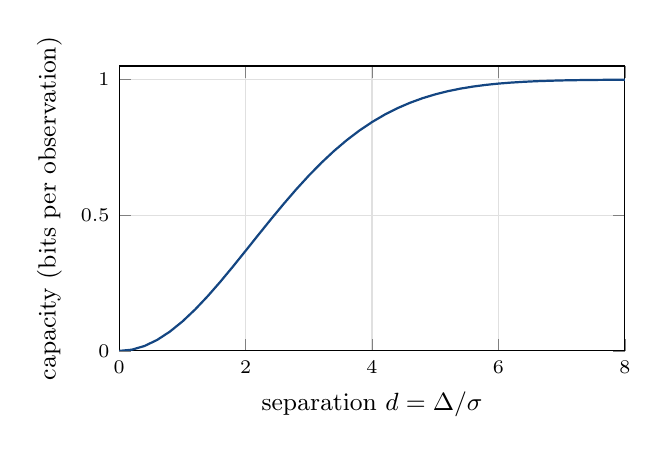
\begin{tikzpicture}
\begin{axis}[width=0.66\linewidth, height=5.2cm, xmin=0, xmax=8, ymin=0, ymax=1.05,
  xlabel={separation $d = \Delta/\sigma$}, ylabel={capacity (bits per observation)},
  tick label style={font=\scriptsize}, label style={font=\small},
  xmajorgrids, ymajorgrids, grid style={draw=black!12}]
\addplot[thick, accent] coordinates {(0.00,0.0000) (0.20,0.0046) (0.40,0.0182) (0.60,0.0405) (0.80,0.0709) (1.00,0.1085) (1.20,0.1525) (1.40,0.2017) (1.60,0.2550) (1.80,0.3111) (2.00,0.3689) (2.20,0.4272) (2.40,0.4850) (2.60,0.5412) (2.80,0.5952) (3.00,0.6461) (3.20,0.6936) (3.40,0.7372) (3.60,0.7767) (3.80,0.8121) (4.00,0.8434) (4.20,0.8707) (4.40,0.8943) (4.60,0.9144) (4.80,0.9314) (5.00,0.9455) (5.20,0.9572) (5.40,0.9667) (5.60,0.9743) (5.80,0.9804) (6.00,0.9852) (6.20,0.9889) (6.40,0.9918) (6.60,0.9940) (6.80,0.9956) (7.00,0.9969) (7.20,0.9978) (7.40,0.9984) (7.60,0.9989) (7.80,0.9992) (8.00,0.9995)};
\end{axis}
\end{tikzpicture}
%% END GENERATED fig_capacity
\caption[Capacity of the hit-or-miss channel]{Capacity of one hit-or-miss
observation against the separation $d = \Delta/\sigma$ of the two latencies,
from \Cref{eq:qerr,eq:bsc}.}
\label{fig:capacity}
\end{figure}

\section{Repetition}

If the same observation can be repeated $n$ times and the results combined by
majority vote, the combined decision is wrong when more than half of the
individual ones are, with probability
\begin{equation}
  \varepsilon_n \;=\; \sum_{k=(n+1)/2}^{n} \binom{n}{k}\,\varepsilon^{k}(1-\varepsilon)^{n-k}
  \qquad (n \text{ odd}).
  \label{eq:majority}
\end{equation}
\Cref{tab:channel} evaluates \Cref{eq:qerr,eq:bsc,eq:majority} for a range of
separations.

\begin{table}[ht]
\centering
\caption[Error, capacity and repetitions of the binary timing channel]{Error
probability of one observation, capacity, and the smallest odd number $n$ of
repetitions for which a majority vote is wrong with probability at most
$10^{-3}$ and $10^{-6}$, for several separations $d$.}
\label{tab:channel}
\footnotesize
%% BEGIN GENERATED tab_channel
\begin{tabular}{@{}rrrrr@{}}
\toprule
$d = \Delta/\sigma$ & $\varepsilon = Q(d/2)$ & $C$ (bits) & $n$ for $10^{-3}$ & $n$ for $10^{-6}$ \\
\midrule
0.5 & 0.4013 & 0.028 & 241 & 569 \\
1.0 & 0.3085 & 0.109 & 61 & 143 \\
2.0 & 0.1587 & 0.369 & 15 & 37 \\
3.0 & 0.0668 & 0.646 & 7 & 17 \\
4.0 & 0.0228 & 0.843 & 5 & 9 \\
6.0 & 0.0013 & 0.985 & 3 & 5 \\
\bottomrule
\end{tabular}
%% END GENERATED tab_channel
\end{table}

Three readings of the table are used in the paper.

\textbf{Large separations need no repetition.} In the model of
\Cref{ch:study} a first-level hit and a second-level hit differ by 10 cycles,
and a first-level hit and a memory access by 216. An observer whose
measurement is uncertain by $\sigma = 2.5$ cycles has $d = 4$ for the smaller
difference, an error of \R{chan.eps.4} per observation and
\R{chan.cap.4} bits of capacity; for the larger difference a single observation
is practically certain.

\textbf{Coarsening the timer costs repetitions, quadratically.} Reducing timer
resolution raises $\sigma$ and lowers $d$. For small $d$ the number of
repetitions needed grows as $1/d^{2}$: halving $d$ from 2 to 1 raises $n$ for
an error of $10^{-6}$ from \R{chan.n6.2} to \R{chan.n6.1}, and halving it again
to \R{chan.n6.0.5}. The channel is slowed, not closed. This is the quantitative
content of the remark in \Cref{sec:primitives}.

\textbf{Capacity is a bound, not a bandwidth.} $C$ is the largest number of bits
that one observation can convey with suitable coding. An attack's rate is $C$
times the number of observations per second, reduced by whatever it must spend
on preparing the state it observes and on waiting for the victim, and it is
further bounded by how much the victim's state depends on the secret at all.
Published rates therefore have to be read with the platform and the
preparation in mind, exactly like the published costs of \Cref{tab:reported}.

\section{What the defences do to the channel}

The model also gives a compact way to say what each defence class of
\Cref{ch:defenses} changes.

\begin{itemize}
  \item \textbf{Isolation} makes the observation independent of the other
        domain: \Cref{eq:ni} holds for the structure that is partitioned or
        flushed, and the capacity of that channel is zero by construction,
        whatever $d$ is.
  \item \textbf{Randomisation} leaves $d$ unchanged but removes the observer's
        knowledge of \emph{which} access to time. The channel exists; using it
        requires a search that the re-keying interrupts (\Cref{app:random}).
  \item \textbf{Hiding or undoing} transient effects removes the dependence of
        the cache state on transient data. The observation of committed
        execution is unaffected, so the ordinary cache channel remains.
  \item \textbf{Restricting} speculation removes the dependence of
        \emph{any} observable on speculatively accessed data, including
        observables other than the cache.
  \item \textbf{Adding noise or coarsening timers} lowers $d$, and
        \Cref{tab:channel} shows what that buys: a polynomial increase in the
        observer's effort.
\end{itemize}

A defence of the first kind can be checked by counting: if no access of one
domain ever changes what the other can observe, the channel is closed. This is
what the interference counts of \Cref{tab:interference} and the invariants of
\Cref{tab:invariants} test for the model.


\chapter{Array Access Time: Where the Latency Gap Comes From}
\label{app:arraymodel}

\Cref{ch:memories} asserted that a larger array is slower, and that the
difference between cache levels is a consequence of how arrays are built. This
appendix gives the first-order argument. It follows the structure of the
analytical model CACTI~\citep{muralimanohar2009cacti}, which estimates the
access time of a cache from its organisation; no numbers are taken from that
tool, only the decomposition.

\section{The components of an access}

A read of the array of \Cref{fig:array} passes through five stages in series,\index{SRAM!access time}
which are the events of \Cref{fig:readtiming}:
\begin{equation}
  t_{\text{access}} \;=\; t_{\text{decode}} + t_{\text{wordline}} + t_{\text{bitline}}
                      + t_{\text{sense}} + t_{\text{output}} .
  \label{eq:taccess}
\end{equation}
Each term scales differently with the number of rows $2^{r}$ and columns
$2^{c}$ of the array.

\textbf{Decode.} Selecting one of $2^{r}$ word lines needs a tree of gates whose
depth grows with $r$, so $t_{\text{decode}} \propto r = \log_2(\text{rows})$.

\textbf{Word line.} The word line runs across every cell of the row. It is a
distributed resistance and capacitance, each proportional to its length, so its
delay grows with the \emph{square} of the number of columns unless it is broken
into segments with repeaters, in which case it grows linearly.

\textbf{Bit line and sensing.} A cell discharges one bit line of the precharged
pair through a deliberately small transistor. The time to develop a voltage
difference $\Delta V$ that the sense amplifier can resolve is
\begin{equation}
  t_{\text{bitline}} \;\approx\; \frac{C_{\text{bl}}\,\Delta V}{I_{\text{cell}}},
  \qquad C_{\text{bl}} \propto \text{rows},
  \label{eq:bitline}
\end{equation}
because every cell in the column adds its drain capacitance to the line. The
cell current $I_{\text{cell}}$ is small by design, since the cell is sized for
density.

\textbf{Output.} The selected bits are driven through the column multiplexer
and, in a cache, through the way multiplexer that the tag comparison controls.
The tag array is read in parallel with the data array, and the comparison of
the stored tag with the address must complete before the correct way can be
selected; in a cache the tag path, not the data path, is usually the critical
one.

\section{Scaling with capacity}

For an array of $N$ bits laid out roughly square, rows and columns both grow
as $\sqrt{N}$. The decoder term then grows as $\log N$ and the wire-dominated
terms as $\sqrt{N}$:
\begin{equation}
  t_{\text{access}}(N) \;\approx\; a + b\,\log_2 N + c\,\sqrt{N}.
  \label{eq:tscale}
\end{equation}
Designers fight the last term by splitting a large array into banks and
sub-arrays, which shortens the lines at the price of extra decoding and wiring
between banks. The square-root growth can be moderated; it cannot be removed,
because the bits have to be somewhere and signals have to travel to them.

Two conclusions matter for this paper.

\textbf{The hierarchy is forced.} A first-level cache must answer within the
few cycles that a load is allowed in the pipeline, which by \Cref{eq:tscale}
caps its size at a few tens of kilobytes. More capacity can only be had
further away and later. The latencies of the model, 4, 14 and 45 cycles for
caches of 32\,KiB, 256\,KiB and 2\,MiB, grow somewhat faster than the square
root of the capacity, because each outer level also adds the cycles needed to
reach it and to return.

\textbf{The gap is robust.} The differences between levels are tens of cycles,
set by geometry and by the distance to the next level. They do not vary from
access to access by anything comparable, which is why the separation $d$ of
\Cref{app:leakage} is large for an observer with a cycle-accurate timer.

\section{Content-addressable arrays and DRAM}

A CAM cell adds a comparison to the storage cell and a match line per entry.
All match lines are evaluated on every lookup, so both the delay and the energy
of a lookup grow with the number of entries, which is why TLBs and the queues
of \Cref{tab:arrayzoo} have tens of entries and not thousands.

A DRAM cell is a capacitor and one transistor. Reading it is destructive, so a
whole row is read into the row buffer and written back; a later access to the
same row is served from the buffer without the activation, and an access to
another row of the same bank must first close the open row. The difference is
again set by the organisation of the array, and it is visible to any program
that shares the memory~\citep{pessl2016drama}.\index{DRAM!row buffer}


\chapter{The RISC-V Privileged Architecture: Three Walk-Throughs}
\label{app:priv}

\Cref{sec:privbrief} named three parts of the privileged
architecture~\citep{riscv-priv} that later chapters rely on. This appendix
walks through each, to make precise what is architectural, and therefore
restored or checked, and what is left to the implementation.

\section{A trap, step by step}

Suppose an instruction in user mode causes an exception that is handled in\index{privilege modes!trap handling}
machine mode. The hardware performs the following steps atomically.

\begin{enumerate}
  \item The address of the faulting instruction is written to \code{mepc}, and
        a code identifying the cause to \code{mcause}; for an access fault the
        offending address may be written to \code{mtval}.
  \item The current interrupt-enable bit and privilege mode are saved in the
        \code{MPIE} and \code{MPP} fields of \code{mstatus}, interrupts are
        disabled, and the mode becomes M.
  \item The program counter is set to the handler address in \code{mtvec}.
\end{enumerate}

The handler saves the integer registers, does its work, restores them and
executes \code{mret}, which reverses step 2 and jumps to \code{mepc}. The trap
is precise: every instruction before the faulting one has completed and none
after it has changed architectural state.

Nothing in these steps mentions a cache, a TLB or a predictor. The instructions
that were in flight behind the faulting one are discarded, and what they did to
\uarchadj{} state is not part of the definition. The handler then runs in the
same caches and trains the same predictors as the code it interrupted, unless
the core or the handler takes explicit action. This is the architectural basis
of scenario S2 in \Cref{tab:threat}.

\section{A PMP check}

Physical memory protection consists of up to 64 entries, each an address\index{physical memory protection (PMP)!matching}
register \code{pmpaddr}$i$ and an 8-bit configuration with read, write and
execute permission bits, an address-matching mode and a lock bit. An entry
matches a range that is either bounded by the previous entry's address (top of
range), a naturally aligned four-byte region, or a naturally aligned power-of-two
region whose size is encoded in the low bits of the address register. For an
access in S or U mode the entries are examined in order, the lowest-numbered
matching entry decides, and if no entry matches the access fails.

As an example, an entry with matching mode NAPOT and
$\code{pmpaddr} = \code{0x2000\_0FFF}$ covers the 32\,KiB region starting at
physical address \code{0x8000\_0000}: the address register holds the address
shifted right by two bits, and its twelve trailing one bits encode a region of
$2^{12+3}$ bytes. With permission bits R and W set and X clear, a user-mode load
from \code{0x8000\_1000} is permitted and an instruction fetch from the same
address raises an access fault.

The check produces one bit: fault or no fault. The specification defines what
happens architecturally when the bit is set. It does not define whether the
data of the load has already been read from the cache and passed to later
instructions by the time the fault is taken. A core that gates forwarding on
the check is not exposed to Meltdown-type leaks; one that does not is, and both
conform (\Cref{tab:variants}).

\section{An Sv39 translation}

Sv39 translates a 39-bit virtual address through a three-level table. The\index{paging!Sv39 walk}
address is split into three 9-bit virtual page numbers and a 12-bit offset;
\code{satp} holds the mode, a 16-bit address-space identifier and the physical
page number of the root table. \Cref{tab:sv39walk} follows the virtual address
\code{0x8020\_1ABC}.

\begin{table}[ht]
\centering
\caption[An Sv39 page-table walk]{The walk for virtual address
\code{0x8020\_1ABC} under Sv39. Each step is one load of an 8-byte page-table
entry; the physical page number found in it is the base of the next table.}
\label{tab:sv39walk}
\footnotesize
\begin{tabularx}{\linewidth}{@{}llX@{}}
\toprule
\textbf{Field} & \textbf{Value} & \textbf{Use} \\
\midrule
VPN[2] = bits 38--30 & 2 & Entry 2 of the root table, at
$\code{satp.PPN} \times 4096 + 2 \times 8$ \\
VPN[1] = bits 29--21 & 1 & Entry 1 of the second-level table that the first
entry points to \\
VPN[0] = bits 20--12 & 1 & Entry 1 of the third-level table; it is a leaf and
holds the physical page number \\
Offset = bits 11--0 & \code{0xABC} & Added to the physical page number shifted
left by 12 \\
\bottomrule
\end{tabularx}
\end{table}

A translation that misses the TLB therefore costs three loads before the load
that the program asked for can begin, and those loads go through the data
caches like any others. The model implements exactly this: its TLB miss
triggers three page-table loads whose latencies are added to that of the data
load, which is the ``walk'' column of \Cref{tab:baseline}. A core with a
page-walk cache skips the upper levels when it has seen them recently, which
is faster and is one more structure with history.

Two details matter for security. A leaf entry at an upper level maps a large
page of 2\,MiB or 1\,GiB, which reduces TLB pressure and also removes the
address bits that page colouring relies on (\Cref{sec:partitioning}). And the
address-space identifier in \code{satp} tags TLB entries, so that the operating\index{address-space identifier (ASID)!and the TLB}
system can switch address spaces without flushing; \code{sfence.vma}
invalidates entries by address, by identifier or both when a mapping changes or
an identifier is reused. Entries of an address space that is not running stay
in the TLB by design. Whether another process can detect them, by the
evictions they cause or suffer, is the TLB channel of \Cref{sec:vm}, and the
``TLB'' columns of \Cref{tab:interference} count the opportunity for it.


\chapter{Pipeline Timing: Worked Examples and the Window Bound}
\label{app:pipeline}

This appendix works three timing examples by hand. The first two concern the
five-stage pipeline of \Cref{fig:pipeline}; the third derives the bound of
\Cref{eq:window} and checks it against the rules of the model.

\section{A load followed by its use}

In the five-stage pipeline a load produces its value at the end of the memory\index{pipeline!load-use hazard}
stage. An instruction that uses the value immediately needs it at the start of
its execute stage, which would be the cycle in which the load is still in
memory access. Forwarding cannot move data backwards in time, so the pipeline
inserts one bubble:

\begin{center}
\footnotesize
\begin{tabular}{@{}lccccccc@{}}
\toprule
\textbf{Cycle} & 1 & 2 & 3 & 4 & 5 & 6 & 7 \\
\midrule
\code{ld   t0, 0(a0)}  & IF & ID & EX & MEM & WB &    &    \\
\code{add  t1, t0, t2} &    & IF & ID & --  & EX & MEM & WB \\
\bottomrule
\end{tabular}
\end{center}

The cost is one cycle per load-use pair, visible in the execution time. If the
load misses the cache the whole pipeline waits for the data, and the wait is
the miss latency. The time a program takes thus already depends on the
addresses it loads from, before any speculation is involved.

\section{A mispredicted branch}

A conditional branch is resolved in the execute stage. If the fetch stage
guessed wrongly, the two instructions fetched behind the branch are discarded
and fetch restarts at the correct target (\Cref{fig:squash}): the penalty is
two cycles, and the two discarded instructions got no further than decode. On
this machine a wrong-path load never reaches the memory stage, so it cannot
touch the data cache. The window exists; it is too short to do anything with.

\section{The window of an out-of-order core}

In an out-of-order core the distance between the stage that fetches and the\index{speculation window!bound}
point where a branch is resolved is not fixed. Let a mispredicted branch be
dispatched into the reorder buffer at time $t_d$ and resolved at $t_r$. From
$t_d$ until $t_r$ the front end keeps delivering instructions along the
predicted path at up to $W$ per cycle, and each needs a free reorder-buffer
entry. The number of wrong-path instructions that enter the window is
therefore at most
\[
  N_{\text{transient}} \;\le\; \min\bigl(R,\; W\,(t_r - t_d)\bigr),
\]
which is \Cref{eq:window}. Of these, an instruction \emph{executes} only if its
operands are ready and it is issued before $t_r$.

The resolution time is $t_r = t_{\text{issue}} + 1$ for a branch, and the
branch issues when its operands are ready. Two cases bracket the range.

\textbf{Operands ready.} If the compared registers were computed long ago, the
branch issues in the cycle after dispatch and resolves one cycle later:
$t_r - t_d = 2$, and at most $2W$ instructions follow it into the window. With
$W = 4$ that is eight instructions, however large the reorder buffer.

\textbf{Operand from a load.} If the branch compares a value that a load is
still fetching, it cannot issue until the load completes. For a load served by
the last-level cache that is 45 cycles in the model, and by memory 220. At
four instructions per cycle the front end could deliver 180 or 880
instructions in that time, so the reorder buffer becomes the limit: $R = 128$
instructions enter the window.

This is why \Cref{fig:window} has two regimes. For \code{bsearch}, whose every
branch compares a freshly loaded key, the number of transient instructions
grows with the reorder buffer up to the point where the kernel's own loop
structure limits it. For kernels whose branches depend on loop counters the
curves are flat: the buffer is never the constraint.

\section{The always-mispredicted branch in the model}

The simplest check of these rules is unit test 14 of \Cref{tab:unit}: a
three-instruction loop whose backward branch is predicted not taken every
time. By the rules of \Cref{app:model}, the three instructions of one
iteration are dispatched in the same cycle $t_d$. The decrement issues at
$t_d + 1$ and completes at $t_d + 2$; the branch needs its result, issues at
$t_d + 2$ and resolves at $t_d + 3$. Fetch is redirected in the next cycle,
$t_d + 4$, and the first instruction of the next iteration is dispatched four
cycles of front-end depth later, at $t_d + 8$. Each iteration therefore takes
exactly eight cycles, and ten when the front-end depth is set to six. The
simulator reports 8.000 and 10.000.


\chapter{Branch Predictors in Detail}
\label{app:predictors}

\Cref{sec:bp} introduced the three prediction structures. This appendix
describes how each works, how the model implements it, and what it means for
two contexts to share one.

\section{The two-bit counter}

A direction predictor entry is a saturating counter with four states: strongly\index{branch prediction!two-bit counter}
not taken, weakly not taken, weakly taken, strongly taken. The prediction is
``taken'' in the upper two states. A taken branch increments the counter and a
not-taken branch decrements it, without wrapping~\citep{smith1981study}. Two
bits instead of one give hysteresis: the single not-taken outcome at the end
of a loop moves the counter from strongly to weakly taken and does not flip the
prediction for the next execution of the loop. A loop of $n$ iterations is
then mispredicted once per execution instead of twice.

\section{Indexing with history}

A table of counters indexed by the low bits of the program counter (a
\emph{bimodal} predictor) gives each branch one counter and cannot learn
patterns. The \emph{gshare} scheme indexes the table with the exclusive-or of\index{branch prediction!gshare}
the program counter and a global history register that holds the outcomes of
the most recent branches~\citep{mcfarling1993combining}. A branch then has a
different counter for each recent history, so an alternating branch, or one
correlated with an earlier branch, becomes predictable. \Cref{tab:predictor}
shows the difference on \code{fibcall}: its base-case test alternates with the
recursion, and the bimodal predictor mispredicts half of the time where gshare
learns the pattern. BOOM's predictor~\citep{seznec2006case,zhao2020sonicboom}
extends the idea with several tables indexed by histories of geometrically
increasing length, with tags to tell colliding branches apart.

Hashing has a cost: two different (branch, history) pairs can select the same\index{predictor!aliasing}
counter. In a table of $2^{n}$ counters that $B$ pairs use uniformly at
random, a given pair shares its counter with at least one other with
probability
\begin{equation}
  1 - \left(1 - 2^{-n}\right)^{B-1} \;\approx\; \frac{B-1}{2^{n}} \quad (B \ll 2^{n}).
  \label{eq:alias}
\end{equation}
Aliasing between the branches of one program costs accuracy. Aliasing between
the branches of two programs is the same event seen as a security property: a
counter trained by one context is used to predict a branch of another.

\section{Targets and returns}

The direction is not enough: the fetch stage also needs the target, and before
decode it does not even know that an instruction is a branch. The \emph{branch
target buffer} caches, per branch address, the target of the last taken\index{branch target buffer (BTB)!operation}
execution. In the model it has 512 direct-mapped entries tagged with the full
address, and a taken branch or jump that is not found costs a short redirect
when decode computes the target.

Returns are predicted by a \emph{return-address stack}: a call pushes the\index{return address stack (RAS)!operation}
address after itself, a return pops. The stack predicts perfectly while the
call depth stays within its capacity; when the stack overflows the oldest
entries are overwritten and the corresponding returns mispredict. With sixteen
entries, \code{fibcall}, which recurses to depth 25, mispredicts fewer than a
hundred of its quarter of a million returns, because deep excursions are rare.

\section{Sharing between contexts in the model}

With two domains on one core the model records, for every prediction, whether
the entry consulted was last written by the other domain, and at every switch
how many entries of each table the outgoing domain owns
(\Cref{tab:interference}). Three policies are available.

\begin{itemize}
  \item \textbf{Shared}, the default: one pattern table, one history register,
        one target buffer and one return stack for both domains.
  \item \textbf{Flushed}: all four are reset at every switch. Nothing is
        inherited, and each domain pays for retraining after every switch.
  \item \textbf{Partitioned}: each domain owns half of the pattern table and of
        the target buffer and has its own history register and return stack.
        Nothing is inherited or lost at a switch, and each domain predicts
        with half the table, permanently.
\end{itemize}

The two isolating policies show the same trade-off as for caches. Flushing
costs per switch; partitioning costs capacity. For the kernels of this study
the predictor part of either cost is small, because the kernels have few
static branches and a table of 2048 counters is ample; a program with thousands
of active branches would feel the halved table through \Cref{eq:alias}.


\chapter{Cache Organisation: Worked Examples}
\label{app:caches}

This appendix works through the cache mechanics that \Cref{ch:memsys} uses:
the address split of the three caches of the model, the replacement policy,
and a numerical instance of \Cref{eq:amat}.

\section{The address split of the model's caches}

A cache of capacity $C$ bytes with associativity $W$ and lines of $B$ bytes has\index{cache!organisation of the model}
$C/(W B)$ sets. The offset field has $\log_2 B$ bits, the index field
$\log_2$ of the number of sets, and the tag is the rest of the address. One way
covers $C/W$ bytes, and with pages of 4\,KiB the cache offers $C/(W \cdot 4096)$
page colours. \Cref{tab:geometry} gives these quantities for the model.

\begin{table}[ht]
\centering
\caption[Geometry of the caches of the model]{Geometry of the caches of the
model for 64-byte lines and a 40-bit physical address. The last column is the
number of page colours with 4\,KiB pages.}
\label{tab:geometry}
\footnotesize
\begin{tabular}{@{}lrrrrrrr@{}}
\toprule
\textbf{Cache} & \textbf{Size} & \textbf{Ways} & \textbf{Sets} & \textbf{Index bits} & \textbf{Tag bits} & \textbf{Way size} & \textbf{Colours} \\
\midrule
First level (I and D) & 32\,KiB  & 8  & 64   & 6  & 28 & 4\,KiB   & 1 \\
Second level          & 256\,KiB & 8  & 512  & 9  & 25 & 32\,KiB  & 8 \\
Last level            & 2\,MiB   & 16 & 2048 & 11 & 23 & 128\,KiB & 32 \\
\bottomrule
\end{tabular}
\end{table}

Take the physical address \code{0x80\_1235\_D678}. Its low six bits,
\code{0x38}, are the offset within the line. Of the bits above them, the
lowest six select set \code{0x19} of the first-level cache, the lowest nine
set \code{0x159} of the second level, and the lowest eleven set \code{0x759}
of the last level.
The three caches are indexed by overlapping bit fields of one address, so two
addresses that collide in a set of the last-level cache also collide in the
second and first levels, but not conversely.

The first row explains two facts used in the text. The index of the
first-level cache lies entirely within the page offset, so it can be indexed
with the virtual address while the TLB is consulted, which is why first-level
caches are built with ways of exactly one page. For the same reason the
operating system has no influence on which first-level set a page occupies: it
has one colour.

\section{Replacement}

When a set is full, a fill must evict one of its lines. The model uses exact\index{replacement policy!LRU and its approximations}
least-recently-used replacement: every access stamps its line with a counter,
and the line with the oldest stamp is evicted. Exact LRU for $W$ ways needs to
order them, which takes $\lceil \log_2 W! \rceil$ bits per set: 16 bits for
eight ways, 45 for sixteen. Hardware therefore usually approximates it with a
binary tree of $W - 1$ bits per set, in which each bit points away from the
half of the set that was used more recently; an access flips the bits on its
path, and the victim is found by following the bits.

For an observer the policy matters because it determines \emph{which} line a
fill displaces. Under exact LRU, filling a set with $W$ fresh lines is
guaranteed to displace everything that was there. Under the tree
approximation the same is true after at most a few more accesses. Under random
replacement it is true only with a probability that approaches one as more
lines are brought in: after $k$ fills a given old line survives with
probability $(1 - 1/W)^{k}$, which for $W = 8$ is still 26\pc{} after ten fills
and 7\pc{} after twenty.

Unit tests 11 to 13 of \Cref{tab:unit} exercise the policy of the model. Eight
lines that map to one first-level set fit, and a loop over them takes four
cycles per load. A ninth line makes every access miss the first level under
LRU, because the line needed next is always the least recently used one, and
the loop takes fourteen cycles per load, the latency of the second level.
Doubling the associativity makes the nine lines fit again.

\section{A numerical instance of the access-time equation}

For \code{bsearch} the model serves \R{base.bsearch.l1_pct}\pc{} of loads from the
first level. \Cref{eq:amat} with the service shares of \Cref{tab:baseline}
gives \R{base.bsearch.amat_formula} cycles, the model's mean load latency is
\R{base.bsearch.mean_load_latency} cycles, and the difference is
\R{base.bsearch.walk_per_load} cycles of page walk and
\R{base.bsearch.wait_per_load} cycles of waiting for lines in flight per load.
The kernel searches a 512\,KiB table. Its first probes hit a few hot lines near
the middle of the table, which stay in the first level; the later probes land
on lines that only the last level holds. Halving the second level to 128\,KiB
would move part of the middle probes outwards, and \Cref{eq:amat} says what
that costs: every per cent of loads that moves from the second level to the
last costs $0.01 \times 31 = 0.31$ cycles per load, and every per cent that
moves from the last level to memory costs 1.75.

That arithmetic is the whole cost model of partitioning. A partition does not
slow anything down by itself; it changes the miss rates, and the hierarchy
multiplies each change by the distance to the next level. Because the distance
to memory is more than five times the distance to the last level, losing capacity at the
last level is far more expensive than losing it further in, which is what
\Cref{tab:isolation} shows for the pairs that no longer fit.

\section{Inclusion}

A hierarchy is \emph{inclusive} if every line in an inner cache is also in the\index{cache!inclusion policies}
outer ones, \emph{exclusive} if a line is in exactly one level, and
\emph{non-inclusive} if no relation is enforced. Inclusion simplifies
coherence, since the outer cache knows everything the inner ones hold, and it
means that evicting a line from the outer cache must evict it from the inner
ones too. The model fills every level on a miss and does not enforce
inclusion on eviction, so it is non-inclusive; it has a single core, and the
cross-core consequence of inclusion discussed in \Cref{ch:memsys} does not
arise in it.


\chapter{Cache Coherence: A Protocol Walk-Through}
\label{app:coherence}

\Cref{sec:coherence} used two properties of coherence protocols: that
transitions differ in cost, and that a write by one core is felt by the others.
This appendix walks through the MESI protocol to show where both come from.
The presentation follows the standard
treatment~\citep{nagarajan2020primer} and textbook \SecRef{12.4.2}.

\section{States and invariant}

Each cache holds each line in one of four states. \emph{Modified}: this cache\index{cache coherence!MESI states}
has the only copy and it differs from memory. \emph{Exclusive}: this cache has
the only copy and it is clean. \emph{Shared}: one or more caches hold a clean
copy. \emph{Invalid}: the cache holds no usable copy. The invariant is single
writer or multiple readers: at any time either one cache holds the line in M or
E, or any number hold it in S.

\section{Transitions and their cost}

\Cref{tab:mesi} lists what happens on a read or a write by the local core, as a
function of the state of the line in the local cache and elsewhere. The last
column is what the access costs beyond a first-level hit.

\begin{table}[ht]
\centering
\caption[MESI transitions and their cost]{MESI transitions for an access by the
local core. ``Elsewhere'' is the strongest state in which any other cache holds
the line.}
\label{tab:mesi}
\footnotesize
\begin{tabularx}{\linewidth}{@{}lll>{\raggedright\arraybackslash}Xl@{}}
\toprule
\textbf{Access} & \textbf{Local} & \textbf{Elsewhere} & \textbf{Action} & \textbf{New state} \\
\midrule
Read  & M, E or S & any  & None: served locally. & unchanged \\
Read  & I & none & Fetch from memory or the outer cache. & E \\
Read  & I & S    & Fetch; a copy may be supplied by the outer cache. & S \\
Read  & I & E    & The owner is asked to downgrade to S. & S \\
Read  & I & M    & The owner must supply the line or write it back, then
downgrade. & S \\
\addlinespace
Write & M & --   & None. & M \\
Write & E & --   & None: the upgrade is silent. & M \\
Write & S & S    & Invalidate all other copies, wait for acknowledgements. & M \\
Write & I & any  & Fetch with intent to write; all other copies are
invalidated. & M \\
\bottomrule
\end{tabularx}
\end{table}

Four costs can be read off the table, in increasing order: nothing; a fetch
from the outer cache; a round trip to another core to downgrade or invalidate
its copy; and a transfer of data that exists only in another core's cache. The
Exclusive state exists to make the common case cheap, a private line that is
read and then written, by making the upgrade from E to M silent.

\section{Why this is observable}

Consider two cores that both have access to one physical line, for instance in\index{cache coherence!as a channel}
a shared library.

\textbf{Reads versus writes.} If the first core only read the line, both hold
it in S and a read by the second is a local hit. If the first core wrote it,
the first holds it in M and the second holds it Invalid: the second core's read
needs the transfer of the fifth row of \Cref{tab:mesi}. The latency of one read
by the second core therefore reveals whether the first core wrote since the
second last looked.

\textbf{Invalidation.} If the second core holds the line in S and the first
writes it, the second core's copy is invalidated (eighth row). The second core
did nothing and its cache content changed; its next access misses. No
capacity pressure and no eviction set are involved.

Neither effect is a flaw in the protocol. Coherence is a correctness
requirement, and the invariant cannot be maintained without telling other
caches about writes. A defence has to remove the sharing of the line (no shared
writable or even readable pages across domains) or accept the channel.

\section{Directories and open RISC-V systems}

With more than a few cores the protocol is implemented with a directory, kept
with the shared cache, that records which cores hold each line, so that
requests go only to the caches concerned. The directory is itself an array
with limited associativity, and evicting a directory entry forces the lines it
tracks out of the private caches. Yan \etal{} showed that this couples the
private caches of different cores even when the data arrays are not
inclusive~\citep{yan2019attack}.

In the open RISC-V ecosystem the cores generated by Rocket
Chip~\citep{asanovic2016rocket} communicate with the rest of the system over
the TileLink interconnect, whose cached variant implements exactly this kind of
permission transfer between a cache and its parent: a cache acquires read or
write permission on a block, and the parent probes other holders to revoke
theirs. The states and costs of \Cref{tab:mesi} therefore apply to those
systems directly. The model of this paper has one core and no coherence
traffic; this appendix is background for \Cref{ch:multicore}, not a description
of the model.


\chapter{Isolation Mechanisms in Detail}
\label{app:isolation}

This appendix describes the three isolation mechanisms of
\Cref{sec:isolation} at the level at which the model implements them, and
derives the cost model for each.

\section{Way partitioning}

A way-partitioned cache gives every security domain a mask over the ways of\index{cache partitioning!way partitioning in the model}
each set. Three operations must respect the mask for the isolation to be
complete, and DAWG~\citep{kiriansky2018dawg} is the design that covers all
three.

\begin{itemize}
  \item \textbf{Fills.} A domain may place a new line only in its own ways.
        This alone prevents one domain from evicting another's lines, and is
        what commercial cache-allocation features provide.
  \item \textbf{Hits.} A domain may hit only on lines in its own ways.
        Otherwise a line cached by one domain would be a hit for another, which
        is the shared-memory channel in a different guise.
  \item \textbf{Replacement metadata.} The recency state of a set must be kept
        per domain, or one domain's accesses would steer another's evictions.
\end{itemize}

The model implements all three: lookup, victim selection and recency are
restricted to the half of the ways that belongs to the running domain, in both
first-level caches, the second level and the last level, and the TLB and the
predictor tables are halved likewise. The interference counts of
\Cref{tab:interference} are then zero by construction, and the invariant test
of \Cref{tab:invariants} confirms that the implementation achieves this.

The cost is that each domain sees caches of half the associativity and half the
capacity: four ways of 16\,KiB at the first level, four ways of 128\,KiB at the
second, eight ways of 1\,MiB at the last, and sixteen TLB entries. What that
costs a given program is read from \Cref{fig:l1sweep,fig:llcsweep}, and it is
paid whether or not another domain is running.

\section{Page colouring}

Colouring restricts the page frames a domain may receive so that the frame\index{page colouring!in the model}
number, in the bits that reach into the cache index, differs between domains.
\Cref{tab:geometry} gives the number of colours of each cache. The model splits
the colours by the lowest bit of the frame number: one domain receives even
frames, the other odd. In the second and last levels each domain can then
reach half of the sets; in the first level, which has one colour, nothing
changes.

Three properties distinguish colouring from way partitioning. It needs no
hardware. It halves the number of \emph{sets} a domain can use and keeps the
associativity, which is gentler on programs with conflict misses and harsher on
programs whose pages are few and hot. And it does nothing for the first-level
caches, the TLB or the predictors, which is why \Cref{tab:interference} shows
the first-level and TLB evictions unchanged under colouring alone. With pages
larger than a cache way there are no colours to distribute, so a system that
uses 2\,MiB pages cannot colour a cache whose ways are 128\,KiB.

\section{Flushing at a switch}

Temporal isolation clears a structure when the running domain changes. The\index{flushing!in the model}
model can flush the first-level caches, the TLB, the predictors, and optionally
the outer caches; the experiments flush the on-core state, as \code{fence.t}
does, and leave the outer caches to colouring. A real implementation must also
make the \emph{duration} of the flush independent of the state being flushed,
since otherwise the time taken would itself reveal how much the previous
domain had touched; a write-back cache, for example, has a variable number of
dirty lines to write. Wistoff \etal{} address this by padding the switch to a
worst-case time~\citep{wistoff2023systematic}. The model charges a constant.

The cost has two parts. The direct part is the flush itself, 322 cycles in the
model. The indirect part is the refill: after the switch the incoming domain
finds an empty first-level cache, TLB and predictor, and every line, page and
branch it touches for the first time costs a miss that the unflushed machine
would not have had. If the domain touches $n_1$ distinct lines that it would
otherwise have found in the first level, each now served by the second level,
the refill costs about $n_1 \Delta_2$ cycles, plus the page walks for the
pages it touches and the mispredictions of the branches it retrains:
\begin{equation}
  c_{\text{switch}} \;\approx\; c_{\text{flush}} + n_1\,\Delta_2
       + n_{\text{pages}}\,t_{\text{walk}} + n_{\text{br}}\,t_{\text{mispredict}} .
  \label{eq:switchcost}
\end{equation}
With $\Delta_2 = 10$ cycles, a first-level data cache of 512 lines bounds the
second term at about 5000 cycles, and the instruction cache adds a smaller
amount of the same kind. The measured totals of \Cref{fig:flushq}, between
\R{flush.perswitch.min} and \R{flush.perswitch.max} cycles, are of that order;
the largest belongs to a pair whose data-dependent branches must also be
learned again after every flush. The relative cost is $c_{\text{switch}}$ divided by the length of
the time slice (\Cref{app:metrics}).

\section{Which mechanism for which structure}

The three mechanisms are complements, not alternatives, and the arithmetic
above assigns each its place. The first-level caches, the TLB and the
predictors are small: they are cheap to flush and painful to halve, and the
first-level cache cannot be coloured at all. The last-level cache is large: it
is expensive to flush, since refilling 2\,MiB from memory costs tens of
thousands of misses at 220 cycles each, and cheap to colour if the working
sets leave room. Flushing the core and colouring the outer caches is therefore
the natural division, and it is the one that the temporal-partitioning work on
CVA6 adopts~\citep{wistoff2023systematic}.


\chapter{Randomised Caches in Detail}
\label{app:random}

\Cref{sec:randomisation} described randomised caches as a race between the
search for conflicting lines and the change of key. This appendix gives the
mechanism as the model implements it, the arithmetic of the race, and one side
effect that the model makes visible.

\section{Encrypted index and gradual remapping}

In a conventional cache the set is selected by the index bits of the line\index{cache!randomisation}
address. In CEASER~\citep{qureshi2018ceaser} the line address is first
encrypted with a secret key by a low-latency block cipher, and the set is
selected by bits of the ciphertext. Which addresses collide then depends on the
key, and an observer who does not know the key cannot compute an eviction set
from addresses.

The key cannot stay fixed, because collisions can be found by experiment. Nor
can it be changed all at once, because every line would then be in the wrong
set. CEASER changes it gradually. It keeps a current key, a next key and a
pointer. Periodically the lines of the set under the pointer are moved to the
sets that the next key assigns them, and the pointer advances; a lookup uses
the next key for an address whose current-key set lies below the pointer and
the current key otherwise. When the pointer has passed every set, the next key
becomes the current one and a fresh key is drawn. One \emph{epoch}, the time to
remap the whole cache, is the lifetime of a key.

The model implements this scheme for the last-level cache, with a 64-bit mixing
function standing in for the cipher. It remaps one set every 1600 accesses to
that level by default, which for 16 ways corresponds to CEASER's default rate
of one remapped line per hundred accesses, and charges two additional cycles
per access for the cipher, the latency CEASER assumes.

\section{The arithmetic of the race}

Let the cache have $S$ sets of $W$ ways. Under a random mapping, an address\index{re-keying rate!arithmetic}
chosen by the observer falls into a particular set with probability $1/S$. To
have $W$ addresses that share a set with a target line, the observer must on
average examine $S \cdot W$ candidates, and must test each for a collision
with the target. For the last-level cache of the model that is
$2048 \times 16 = \num{32768}$ candidates.

How many memory accesses the testing takes depends on the algorithm. A
straightforward search tests candidates in a way that costs a number of
accesses quadratic in the size of the pool; group-testing methods reduce this
to a number linear in it~\citep{vila2019theory}; and methods that exploit the
structure of a particular randomised design reduce it
further~\citep{qureshi2019ceasers,purnal2021systematic}. The defence holds as
long as an epoch contains fewer accesses than the search needs. At one remapped
set per 1600 accesses an epoch of the model's cache is
$2048 \times 1600 \approx 3.3$ million accesses to the last level.

This is why the class has needed repeated revision. The original remapping
rate was chosen against the quadratic search; the linear search made it
inadequate, and the response was either to remap far more often, which costs
performance, or to change the design so that a single key no longer determines
a single set. ScatterCache and the skewed variant of
CEASER~\citep{werner2019scattercache,qureshi2019ceasers} use a different
mapping per way, so that two addresses rarely collide in all ways, and
MIRAGE~\citep{saileshwar2021mirage} arranges that a fill almost never evicts a
line because of a set conflict at all.

\section{What remapping costs in the model}

\Cref{tab:random} in \Cref{app:results} gives the cost for each kernel at four
remapping rates. At the default rate the geometric-mean slowdown is
\R{rand.1600.geo}\pc{} and the worst case \R{rand.1600.worst}\pc{}, consistent
in magnitude with the roughly one per cent that CEASER reports for its own
workloads. Remapping sixteen times as often raises the worst case to
\R{rand.100.worst}\pc{}: each remapped set displaces lines that then have to be
fetched again. The dependence on the rate is steep, which is the performance
side of the race.

\section{A side effect: random placement and conflict misses}

The model shows one effect that is easy to overlook. A random mapping
distributes lines over sets like balls thrown into bins. If a program's working
set occupies a fraction $\rho$ of the cache, the number of its lines that fall
into a given set is approximately Poisson distributed with mean $\rho W$, and
sets that receive more than $W$ lines overflow even though the cache as a
whole has room. For $W = 16$ and $\rho = 0.5$ the mean is 8 and the probability
that a set overflows is under one per cent; for $\rho = 0.8$ the mean is 12.8
and about 15\pc{} of the sets overflow. A conventional cache with well-placed
pages would hold the same working set without a single conflict.

The effect appears in the column of \Cref{tab:random} for a static key with no
added latency, which isolates it: \code{listwalk}, whose list fills half of the
last-level cache, runs about 3\pc{} slower under the hashed mapping than under
the direct one, purely from conflicts, while \code{stream} happens to run
slightly faster, because the hash spreads its lines better than the page layout
it replaces. It also explains part of the spread over
page-frame layouts in \Cref{tab:isolation}, because an operating system that
hands out page frames without regard to colour produces the same kind of
random placement at the granularity of a page.


\chapter{The Modelled Speculation Defences}
\label{app:specdef}

\Cref{sec:defcost} reported the cost of seven speculation defences. This
appendix states the rule that each one adds to the model of \Cref{app:model},
on the committed path and on the wrong path, and says which published design
supplied the idea and what of that design is left out. The mechanisms are named
after what they do, not after the designs, to keep the two apart.

\section{The visibility point}

Every mechanism is defined relative to the \emph{visibility point} of an\index{visibility point}
instruction: the time from which it can no longer be squashed. Following the
literature~\citep{yan2018invisispec,yu2019stt}, two attack models give two
definitions.

\begin{itemize}
  \item \textbf{Spectre model.} Only control-flow mispredictions squash. An
        instruction reaches its visibility point when every older conditional
        branch and indirect jump has resolved.
  \item \textbf{Futuristic model.} Anything may squash. An instruction reaches
        its visibility point when every older instruction has finished
        executing.
\end{itemize}

In the model the first is the latest resolution time of any older control
transfer and the second the latest completion time of any older instruction. A
load is \emph{speculative} if it issues before its visibility point. On a
wrong path the visibility point never arrives: the mispredicted branch is
older than every wrong-path instruction and has, by definition, not resolved.

\section{The seven rules}

\Cref{tab:specrules} gives the rules. The left column of rules changes the
timing of committed instructions and is where the cost comes from. The right
column decides what the wrong path may do and is where the protection comes
from.

\begin{table}[ht]
\centering
\caption[Rules of the modelled speculation defences]{The modelled speculation
defences as rules on the timing model. ``VP'' is the visibility point of the
instruction concerned.}
\label{tab:specrules}
\footnotesize
\begin{tabularx}{\linewidth}{@{}l>{\raggedright\arraybackslash}X>{\raggedright\arraybackslash}X@{}}
\toprule
\textbf{Name} & \textbf{Committed path} & \textbf{Wrong path} \\
\midrule
NoSpecLoad &
A load does not issue before its VP. &
No load issues. \\
\addlinespace
DoM &
A load that would miss the first-level cache or the TLB does not issue before
its VP; a load that hits proceeds. &
A load that hits executes, without updating replacement state; a load that
would miss does not issue. \\
\addlinespace
Invis-E &
A speculative load is made visible by a second access at its VP; that access is
counted as traffic and delays nothing. &
Loads execute and read the hierarchy without changing it. \\
\addlinespace
Invis-V &
As Invis-E, and the load does not commit until the second access has completed,
which takes the latency of the level that served the first access, at most
that of the last level. &
As Invis-E. \\
\addlinespace
Taint &
The result of a speculative load is tainted until the load's VP. Taint
propagates through register dependences. A load whose address is tainted does
not issue, and a branch whose operand is tainted does not resolve, before the
taint expires. &
The result of a load is tainted for good; a load with a tainted address never
issues. Other loads execute and fill the cache. \\
\addlinespace
NoFwd &
The result of a speculative load is withheld from dependent instructions until
the load's VP. &
The result of a load is never forwarded. Loads whose address does not depend
on a transient load execute and fill the cache. \\
\addlinespace
Undo &
Unchanged. &
Loads execute; nothing they do to the cache persists. Each first-level fill
that had completed before the squash delays the redirect: restores run four at
a time, each group taking one second-level latency. \\
\bottomrule
\end{tabularx}
\end{table}

\section{Relation to the published designs}

\textbf{NoSpecLoad} is the baseline that the papers on invisible speculation
and on taint tracking compare against under names such as ``fence after every
branch'' or ``delay all speculative loads''. It bounds the cost of the class
from above.

\textbf{DoM} follows delay-on-miss~\citep{sakalis2019delay}. The published
design adds value prediction for the delayed loads, which recovers part of the
loss; the model has none.

\textbf{Invis-E and Invis-V} follow the two ways in which
InvisiSpec~\citep{yan2018invisispec} makes a load visible: an \emph{exposure},
which the load does not wait for, and a \emph{validation}, which it does. The
published design chooses between them per load according to the memory
consistency model, squashes when a validation fails, and keeps speculative
lines in buffers of limited size at the core and at the last-level cache. The
model has none of these, and under the weak memory model of RISC-V most loads
would need only an exposure; the two variants bracket the design.

\textbf{Taint} follows speculative taint tracking~\citep{yu2019stt}: outputs of
speculative accesses are tainted, and only \emph{transmitters} of tainted
values are delayed. The model treats a load address and a branch resolution as
transmitters. The published design also covers the prediction-based implicit
channels and proves non-interference for its rules; the model's version is
checked only by the invariant that no dependent transient load executes.

\textbf{NoFwd} is closest to the least restrictive policy of
NDA~\citep{weisse2019nda}, in which the results of speculative loads do not
propagate. NDA's stricter policies restrict every instruction's result, or do
not let loads execute speculatively at all; the latter coincides with
NoSpecLoad.

\textbf{Undo} follows CleanupSpec~\citep{saileshwar2019cleanupspec}. The
published design invalidates transiently installed lines, restores the lines
they evicted, discards fills that return after the squash, and relies on a
randomised second-level cache to make evictions there harmless. The model
keeps only the first-level rollback and its cost.

\section{What the rules imply}

Three properties follow from the table without any simulation, and each is
verified as an invariant in \Cref{tab:invariants}. Under NoSpecLoad, DoM, the
invisible schemes and Undo no transient load leaves a first-level fill, because
in each case either the load does not issue or its fill is suppressed or
reverted. Under NoSpecLoad, Taint and NoFwd no \emph{dependent} transient load
executes, because its address never becomes available untainted, or at all.
And under Taint and NoFwd the \emph{independent} transient loads still fill
the cache, since their addresses were computed from committed values and the
rules have no reason to stop them.

The last point is the one most easily misread. A taint-tracking scheme does
not promise an unchanged cache. It promises that what the cache reveals about
transient execution does not depend on transiently read data. Whether that is
the right promise depends on whether the addresses of the independent loads
are themselves sensitive, which is the question that separates STT's notion of
a secret from SPT's~\citep{choudhary2021spt}.


\chapter{The Timing Model: Specification}
\label{app:model}

This appendix specifies the timing model of the simulator \code{rvmodel}, whose
source is \Cref{lst:rvmodel}. The functional core needs no specification beyond
the RV64IM instruction set~\citep{riscv-unpriv}; everything below concerns
\emph{when} things happen. The rules are deliberately few, so that each result
of \Cref{ch:tradeoffs} can be traced to one of them.

\section{Times assigned to each instruction}

Instructions are processed in the order in which the functional core executes\index{model study!timing rules}
them, which is program order. Each committed instruction $i$ receives five
times, in cycles: fetch $f_i$, dispatch $d_i$, issue $s_i$, completion $x_i$
and commit $c_i$. Let $W$ be the width, $R$ the number of reorder-buffer
entries and $F$ the depth of the front end.

\textbf{Fetch.} At most $W$ instructions are fetched per cycle. A taken branch
or jump ends the fetch group: the next instruction is fetched one cycle later
if the target was found in the branch target buffer and three cycles later if
it had to be computed at decode. When fetch moves to a new cache line, the line
is looked up in the instruction cache, and a latency above that of a
first-level hit delays fetch by the excess. After a misprediction that resolves
at time $r$, fetch resumes at $r + 1$.

\textbf{Dispatch.} An instruction enters the reorder buffer $F$ cycles after it
is fetched, in order, at most $W$ per cycle, and only when the instruction $R$
places ahead of it has committed:
\begin{equation}
  d_i \;=\; \max\bigl(f_i + F,\; c_{i-R} + 1,\; d_{i-1}\bigr).
  \label{eq:dispatch}
\end{equation}
Fetch may not run more than $F$ cycles ahead of dispatch, so a full reorder
buffer stalls the front end.

\textbf{Issue.} An instruction issues one cycle after dispatch or when its
source registers are ready, whichever is later:
\begin{equation}
  s_i \;=\; \max\bigl(d_i + 1,\; \max_{r \in \text{src}(i)} \text{ready}(r)\bigr).
  \label{eq:issue}
\end{equation}
There is no limit on the number of instructions that issue in a cycle.

\textbf{Completion.} $x_i = s_i + l_i$, where the latency $l_i$ is one cycle for
integer operations, branches and stores, three for multiplication, twenty for
division, and the load latency defined below for loads. The destination
register becomes ready at $x_i$. The link register of a jump is ready at
$d_i + 1$.

\textbf{Commit.} Instructions commit in order, at most $W$ per cycle, no earlier
than the cycle after completion: $c_i = \max(x_i + 1, c_{i-1})$. The cycle count
of a run is the commit time of its last instruction.

\section{Loads, stores and the memory hierarchy}

A load first consults the TLB. On a miss, three page-table entries are loaded\index{model study!memory hierarchy}
one after another through the data caches, at addresses that depend on the
virtual page number as in Sv39, and the sum of their latencies is added to the
load. The data access then looks for the line in the first-level cache, the
second level and the last level in turn. Its latency is that of the first
level in which the line is found, or that of memory. On the way back the line
is filled into every level that missed, each fill evicting the least recently
used line of its set.

Every line carries the time at which its data arrives. A load that finds a
line whose data has not yet arrived waits for it. This models the merging of a
second miss with an outstanding one, and is the ``wait'' column of
\Cref{tab:baseline}.

A store completes one cycle after its operands are ready and accesses the cache
at its commit time; no latency is charged to it, as if it drained from a store
buffer in the background. A load to a doubleword that an older, not yet
committed store has written takes its data from that store, one cycle after
the store's data is ready, without accessing the cache. Loads never issue ahead
of an older store to the same address: memory dependences are assumed to be
known.

Because instructions are processed in program order, the cache is updated in
program order. Two loads that overlap in time see the cache in the order in
which the program contains them, not the order in which they would issue. This
is the main approximation of a trace-driven model.

\section{Prediction}

A conditional branch is predicted from the pattern table and resolves at its
completion time. The table and the history register are updated with the true
outcome when the branch is processed, so the model has no delay between
resolution and update and no pollution of the history by wrong-path branches.
A return is predicted from the return-address stack and any other indirect
jump from the branch target buffer. A direct jump is never mispredicted; if its
target is not in the target buffer it costs the short redirect described under
fetch.

\section{The wrong path}

When a conditional branch or an indirect jump is mispredicted, the simulator\index{model study!wrong-path execution}
executes the wrong path explicitly before continuing with the correct one. It
copies the architectural registers and the register-ready times into scratch
arrays, starts at the predicted target, and executes instructions
functionally, with stores going to a private buffer that later wrong-path loads
consult. Each wrong-path instruction is dispatched in the slot it would have
occupied behind the branch, $W$ per cycle, and receives an issue time by
\Cref{eq:issue}.

A wrong-path instruction is \emph{executed} if it issues before the branch
resolves. An executed wrong-path load accesses the TLB and the caches exactly
as a committed load does, including the fills, unless a defence rule of
\Cref{tab:specrules} says otherwise. Branches on the wrong path follow the
predictor without updating it. The wrong path ends when an instruction would
be dispatched at or after the resolution time, when $R$ instructions have been
dispatched, or when the path leaves the program's memory or reaches an
instruction that the simulator does not execute. The scratch registers and the
store buffer are then discarded.

The simulator tracks, for every scratch register, whether its value derives
from a wrong-path load. A wrong-path load whose address register is so marked
is a \emph{dependent} transient load, the quantity of \Cref{tab:window}.

\section{Two domains}

With two programs the simulator keeps two sets of registers and two memory
images and runs them alternately on the one timing state, switching after a
fixed number of instructions. Each domain's virtual pages are mapped to
physical frames by a fixed pseudo-random bijection, in disjoint frame ranges;
a seed selects the layout. Every cache line, TLB entry and predictor entry
records the domain that wrote it, which is what the interference counts of
\Cref{tab:interference} are computed from. At a switch the configured
structures are flushed, the flush cost is added if any structure is flushed,
and the incoming domain starts with all its registers ready.

\section{What the simulator reports}

For each run the simulator prints the checksum the program wrote to the serial
port, instruction and cycle counts per domain, counts of loads, stores,
branches and mispredictions, accesses and misses at each cache level and in the
TLB, the distribution of load service over the levels with its walk and wait
components, the wrong-path counts, and for two domains the interference and
residue counts. The driver of \Cref{lst:driver} collects these into the result
files from which every table and plot of the study is generated.


\chapter{Validation of the Model}
\label{app:validation}

\Cref{sec:validation} summarised three checks. This appendix gives the method
and the complete results of each, and a fourth check on the influence of the
page-frame layout.

\section{Functional agreement}

Each kernel returns a 64-bit checksum from \code{main}. The start-up code of\index{model study!functional validation}
\Cref{lst:crt} prints it as sixteen hexadecimal digits on the serial port and
switches the machine off. The same binary is run in three ways.

\begin{itemize}
  \item \textbf{QEMU.} The ELF file is loaded with
        \code{qemu-system-riscv64 -machine virt -bios none -kernel}, so that the
        program starts in machine mode at the base of memory with no firmware
        in between. The serial port and the power-off device are those of the
        \code{virt} board.
  \item \textbf{The simulator.} \code{rvmodel} loads the flat image at the same
        address and models the same two devices.
  \item \textbf{A Python reference.} The file \code{reference.py} in the
        repository implements the algorithm of each kernel in ordinary Python,
        with the same pseudo-random input sequence, without any reference to
        RISC-V. For the CRC it uses the library routine of the Python
        distribution.
\end{itemize}

A kernel is accepted only if the three checksums are identical;
\Cref{tab:validation} shows that all are. The check covers the instruction
encodings produced by the assembler (QEMU decodes them independently), the
semantics implemented by the functional core (QEMU executes them
independently), and the kernels themselves (the Python reference computes the
intended result independently). Every instruction that the kernels use, from
the base integer set and from the multiply and divide extension, is exercised
this way. The checksums are designed to depend on the order of the
results, not just on their sum, so that an error is unlikely to cancel.

\section{Timing against hand derivation}

The timing rules are checked differentially. A small loop is run for $n$ and\index{model study!timing validation}
for $2n$ iterations, and the difference in cycle count divided by $n$ is the
steady-state cost of one iteration, free of start-up effects. That cost is
derived by hand from the rules of \Cref{app:model} before the test is run.
\Cref{tab:unit} lists the fifteen tests; the derivations of four representative
ones follow. For these tests the page frames are assigned without scattering,
so that the placement of lines in sets is known exactly.

\begin{table}[ht]
\centering
\caption[Timing unit tests]{Timing unit tests: cycles per loop iteration derived
by hand from the rules of the model, and measured as the difference between
runs of $n$ and $2n$ iterations.}
\label{tab:unit}
\footnotesize
%% BEGIN GENERATED tab_unit
\begin{tabular}{@{}rlrrc@{}}
\toprule
\textbf{\#} & \textbf{Loop body under test} & \textbf{Derived} & \textbf{Measured} & \textbf{Equal} \\
\midrule
1 & 2 independent adds, width 4 & 1.0 & 1.000 & yes \\
2 & 6 independent adds, width 4 & 2.0 & 2.000 & yes \\
3 & 6 independent adds, width 2 & 4.0 & 4.000 & yes \\
4 & chain of 6 dependent adds & 6.0 & 6.000 & yes \\
5 & multiply chain & 3.0 & 3.000 & yes \\
6 & divide chain & 20.0 & 20.000 & yes \\
7 & load chain, first-level hit & 4.0 & 4.000 & yes \\
8 & load chain, second-level hit & 14.0 & 14.000 & yes \\
9 & load chain, last-level hit & 45.0 & 45.000 & yes \\
10 & load chain, memory & 220.0 & 220.000 & yes \\
11 & 8 lines in one 8-way set & 4.0 & 4.000 & yes \\
12 & 9 lines in one 8-way set & 14.0 & 14.000 & yes \\
13 & 9 lines in one 16-way set & 4.0 & 4.000 & yes \\
14 & always-mispredicted branch, depth 4 & 8.0 & 8.000 & yes \\
15 & always-mispredicted branch, depth 6 & 10.0 & 10.000 & yes \\
\bottomrule
\end{tabular}
%% END GENERATED tab_unit
\end{table}

\textbf{Test 2: six independent additions, width four.} The loop body has six
additions whose only source is the zero register, the decrement of the counter
and the branch: eight instructions. Four are fetched per cycle, so an
iteration occupies two fetch cycles, and the taken branch ends the second
group. Nothing else limits the loop, since the only dependence chain is the
counter with one cycle per iteration. Two cycles per iteration.

\textbf{Test 4: a chain of six dependent additions.} Each addition needs the
result of the previous one, one cycle each, and the chain continues into the
next iteration through the same register. The dependence chain, six cycles per
iteration, is longer than the two cycles that fetching takes, so the reorder
buffer fills and the chain sets the pace. Six cycles per iteration.

\textbf{Tests 8 to 10: load chains.} The loop follows a ring of pointers in
which every node is on its own cache line. With 1024 nodes the ring occupies
64\,KiB: twice the first-level cache, so with LRU replacement no node is ever
still in the first level when it is needed again, and well within the second
level. Each load is a first-level miss and a second-level hit, and the next
load cannot issue before its address arrives: fourteen cycles per iteration.
With 8192 nodes the ring exceeds the second level and fits the last, giving 45
cycles; with 65536 nodes it exceeds the last level, giving 220.

\textbf{Tests 11 to 13: contention for one set.} Nodes spaced a page apart have
the same index in the first-level cache. Eight of them fit in the eight ways
of the set and the loop runs at the first-level latency of four cycles. With a
ninth, each access evicts the least recently used node, which is exactly the
one the loop needs next, so each load misses the first level and hits the
second: fourteen cycles. With sixteen ways
the nine nodes fit again.

All fifteen measured values equal the derived ones to the three decimals
printed.

\section{Invariants of the mechanisms}

\Cref{tab:invariants} lists properties that follow from the definitions of the\index{model study!invariants}
mechanisms (\Cref{tab:specrules,app:isolation}) and must therefore hold exactly
in every run. Each was evaluated over the complete runs of all kernels or of a
pair of kernels.

\begin{table}[ht]
\centering
\caption[Invariants of the modelled mechanisms]{Invariants checked on full
runs. The two rows marked ``$> 0$'' confirm that the quantity being eliminated
is present when the mechanism is switched off.}
\label{tab:invariants}
\footnotesize
%% BEGIN GENERATED tab_invariants
\begin{tabularx}{\linewidth}{@{}Xrrc@{}}
\toprule
\textbf{Property} & \textbf{Measured} & \textbf{Required} & \textbf{Holds} \\
\midrule
Transient first-level fills under nospec, all kernels & 0 & 0 & yes \\
Transient first-level fills under dom, all kernels & 0 & 0 & yes \\
Transient first-level fills under invis-e, all kernels & 0 & 0 & yes \\
Transient first-level fills under invis-v, all kernels & 0 & 0 & yes \\
Transient first-level fills under undo, all kernels & 0 & 0 & yes \\
Dependent transient loads executed under nospec, all kernels & 0 & 0 & yes \\
Dependent transient loads executed under stt, all kernels & 0 & 0 & yes \\
Dependent transient loads executed under nda, all kernels & 0 & 0 & yes \\
Dependent transient loads executed with no defence & 7\,221 & > 0 & yes \\
Cross-domain evictions, way partitioning (all levels + tlb) & 0 & 0 & yes \\
Predictions made from the other domain's entries, partitioned predictors & 0 & 0 & yes \\
Cross-domain evictions in l2 and llc, page colouring & 0 & 0 & yes \\
First-level, tlb and predictor residue after a flush & 0 & 0 & yes \\
Predictions made from the other domain's entries, flushed predictors & 0 & 0 & yes \\
Cross-domain evictions with no isolation (first level) & 54\,406 & > 0 & yes \\
Repeatability of cycle count, matmul & 605\,057 & 605057 & yes \\
Repeatability of cycle count, bstree & 9\,476\,276 & 9476276 & yes \\
\bottomrule
\end{tabularx}
%% END GENERATED tab_invariants
\end{table}

The invariants are tests, not proofs: they show that the properties hold on
these runs. They are nevertheless strong evidence that the mechanisms are
implemented as specified, because each is an exact zero over several million
instructions, and a single misplaced update would break it.

\section{Sensitivity to the page-frame layout}

The model assigns page frames pseudo-randomly, as an operating system that has
been running for a while would. The layout decides which pages collide in the
outer caches, so it changes the results. \Cref{tab:seeds} shows by how much,
over five layouts.

\begin{table}[ht]
\centering
\caption[Spread of results over page-frame layouts]{Baseline cycle count of each
kernel over five page-frame layouts, the spread between the fastest and the
slowest as a percentage of the mean, and the range of the slowdown of two
defences over the same layouts.}
\label{tab:seeds}
\footnotesize
%% BEGIN GENERATED tab_seeds
\begin{tabular}{@{}lrrrrr@{}}
\toprule
\textbf{Kernel} & \textbf{Fewest cycles} & \textbf{Most cycles} & \textbf{Spread (\%)} & \textbf{DoM (\%)} & \textbf{Taint (\%)} \\
\midrule
\texttt{matmul} & 605\,057 & 605\,057 & 0.00 & 0.0--0.0 & 0.0--0.0 \\
\texttt{heapsort} & 1\,346\,292 & 1\,346\,541 & 0.02 & 0.7--0.7 & 0.2--0.3 \\
\texttt{listwalk} & 5\,639\,468 & 6\,777\,575 & 19.37 & 1.4--1.8 & 0.0--0.0 \\
\texttt{bsearch} & 5\,371\,712 & 5\,414\,795 & 0.80 & 37.1--37.3 & 5.5--5.7 \\
\texttt{bstree} & 9\,307\,884 & 9\,535\,994 & 2.41 & 1.8--1.9 & 3.0--3.1 \\
\texttt{crc32} & 2\,510\,733 & 2\,511\,229 & 0.02 & 0.0--0.0 & 0.0--0.0 \\
\texttt{sieve} & 1\,019\,522 & 1\,047\,344 & 2.70 & 0.6--1.2 & 0.0--0.0 \\
\texttt{hashtab} & 3\,958\,055 & 4\,135\,552 & 4.36 & 37.5--40.0 & 4.6--5.0 \\
\texttt{stream} & 1\,051\,151 & 1\,271\,297 & 19.10 & 0.0--0.0 & 0.0--0.0 \\
\texttt{fibcall} & 1\,052\,490 & 1\,052\,490 & 0.00 & 0.0--0.0 & 0.0--0.0 \\
\texttt{strsearch} & 1\,484\,894 & 1\,484\,894 & 0.00 & 0.2--0.2 & 0.0--0.0 \\
\bottomrule
\end{tabular}
%% END GENERATED tab_seeds
\end{table}

Kernels that fit in the first two cache levels are insensitive to the layout.
The two whose working sets approach the size of the last-level cache,
\code{listwalk} and \code{stream}, vary by \R{seed.spread.listwalk}\pc{} and
\R{seed.spread.stream}\pc{} in their baseline run time, purely from where their
pages happen to fall; this is the page-placement effect described by Kessler
and Hill~\citep{kessler1992page}. The \emph{slowdown} of a speculation defence
is much more stable than the absolute time, because it is a ratio of two runs
on the same layout. For this reason the single-domain results of
\Cref{ch:tradeoffs} are reported for one layout, and the isolation results,
which depend on capacity, as a mean and range over five.


\chapter{Complete Results of the Model Study}
\label{app:results}

This appendix holds the result tables that the chapters summarise or plot. All
are generated from the result files of the study.

\section{Speculation defences under the Futuristic model}

\Cref{tab:defcostfut} is the counterpart of \Cref{tab:defcost} for the
Futuristic attack model, in which a load is safe only when every older
instruction has completed. The mechanisms that delay loads become far more
expensive, because loads that would have overlapped now wait for one another:
NoSpecLoad turns a four-wide machine into one that issues one load at a time.
The mechanisms that act only at a squash, or only on dependent loads, change
little.

\begin{table}[ht]
\centering
\caption[Slowdown of each speculation defence, Futuristic model]{Slowdown in per
cent of each modelled speculation defence under the Futuristic model, against
the undefended model.}
\label{tab:defcostfut}
\footnotesize
%% BEGIN GENERATED tab_defcost_futuristic
\begin{tabular}{@{}lrrrrrrr@{}}
\toprule
\textbf{Kernel} & \textbf{NoSpecLoad} & \textbf{DoM} & \textbf{Invis-E} & \textbf{Invis-V} & \textbf{Taint} & \textbf{NoFwd} & \textbf{Undo} \\
\midrule
\texttt{matmul} & 427.7 & 0.4 & 0.0 & 0.0 & 0.0 & 79.8 & 0.0 \\
\texttt{heapsort} & 51.8 & 1.6 & $-$0.3 & $-$0.3 & 0.3 & 1.6 & $-$0.2 \\
\texttt{listwalk} & 15.4 & 2.2 & 0.0 & 0.1 & 1.8 & 2.4 & 0.0 \\
\texttt{bsearch} & 43.0 & 37.3 & $-$3.5 & $-$3.5 & 5.6 & 6.3 & 6.9 \\
\texttt{bstree} & 25.9 & 1.9 & 0.0 & 0.0 & 3.1 & 4.0 & 0.0 \\
\texttt{crc32} & 46.1 & 5.0 & 0.0 & 0.0 & 0.0 & 0.0 & 0.0 \\
\texttt{sieve} & 56.0 & 0.8 & 0.4 & 0.4 & 0.0 & 0.7 & 0.4 \\
\texttt{hashtab} & 56.0 & 38.9 & 5.8 & 6.1 & 4.9 & 6.0 & 14.9 \\
\texttt{stream} & 265.8 & 122.0 & 0.0 & 29.8 & 0.0 & 3.9 & 0.0 \\
\texttt{fibcall} & 46.4 & 0.0 & 0.0 & 0.0 & 0.0 & 0.0 & 0.0 \\
\texttt{strsearch} & 57.4 & 0.2 & 0.1 & 0.1 & 0.0 & 0.1 & 0.1 \\
\midrule
\textbf{geometric mean} & \textbf{75.9} & \textbf{15.3} & \textbf{0.2} & \textbf{2.7} & \textbf{1.4} & \textbf{7.8} & \textbf{1.9} \\
worst kernel & 427.7 & 122.0 & 5.8 & 29.8 & 5.6 & 79.8 & 14.9 \\
\bottomrule
\end{tabular}
%% END GENERATED tab_defcost_futuristic
\end{table}

\section{Cache size and associativity}

\Cref{tab:cachesweep} gives the first-level data-cache miss rates that
\Cref{fig:l1sweep} plots for six kernels, for all eleven.

\begin{table}[ht]
\centering
\caption[First-level miss rates for all kernels]{First-level data-cache miss
rate in per cent of all accesses, against cache size at eight ways and against
associativity at 32\,KiB.}
\label{tab:cachesweep}
\footnotesize
%% BEGIN GENERATED tab_cachesweep
\begin{tabular}{@{}l@{\hspace{10pt}}rrrrr@{\hspace{14pt}}rrrrr@{}}
\toprule
 & \multicolumn{5}{c}{\textbf{size in KiB (8 ways)}} & \multicolumn{5}{c}{\textbf{ways (32\,KiB)}} \\
\textbf{Kernel} & \textbf{8} & \textbf{16} & \textbf{32} & \textbf{64} & \textbf{128} & \textbf{1} & \textbf{2} & \textbf{4} & \textbf{8} & \textbf{16} \\
\midrule
\texttt{matmul} & 50.35 & 14.78 & 0.22 & 0.14 & 0.14 & 3.13 & 1.25 & 0.24 & 0.22 & 0.23 \\
\texttt{heapsort} & 8.61 & 6.31 & 4.01 & 1.91 & 0.39 & 6.56 & 4.56 & 4.14 & 4.01 & 4.02 \\
\texttt{listwalk} & 21.27 & 19.67 & 18.90 & 18.42 & 18.34 & 20.58 & 19.31 & 18.98 & 18.90 & 18.90 \\
\texttt{bsearch} & 42.12 & 41.47 & 40.31 & 34.91 & 25.84 & 39.85 & 39.80 & 40.15 & 40.31 & 38.41 \\
\texttt{bstree} & 11.99 & 9.64 & 7.30 & 4.92 & 2.39 & 9.66 & 8.01 & 7.61 & 7.30 & 7.28 \\
\texttt{crc32} & 1.48 & 1.48 & 1.48 & 1.48 & 1.48 & 1.62 & 1.48 & 1.48 & 1.48 & 1.48 \\
\texttt{sieve} & 17.08 & 17.01 & 16.78 & 15.83 & 12.76 & 16.63 & 16.68 & 16.76 & 16.78 & 16.79 \\
\texttt{hashtab} & 25.64 & 24.50 & 22.85 & 19.68 & 13.45 & 23.56 & 23.14 & 22.89 & 22.85 & 22.85 \\
\texttt{stream} & 10.20 & 9.99 & 9.97 & 9.97 & 9.97 & 21.89 & 10.60 & 10.01 & 9.97 & 9.97 \\
\texttt{fibcall} & 0.00 & 0.00 & 0.00 & 0.00 & 0.00 & 0.00 & 0.00 & 0.00 & 0.00 & 0.00 \\
\texttt{strsearch} & 0.78 & 0.78 & 0.78 & 0.78 & 0.52 & 0.92 & 0.78 & 0.78 & 0.78 & 0.78 \\
\bottomrule
\end{tabular}
%% END GENERATED tab_cachesweep
\end{table}

\section{Randomised last-level index}

\Cref{tab:random} gives the cost of the encrypted, gradually remapped index for
each kernel. The column ``Static'' uses a fixed key and no added latency, which
isolates the effect of random placement (\Cref{app:random}); the next four
columns add the two-cycle latency and remap one set every 6400, 1600, 400 and
100 accesses to the last level. The last column counts lines evicted by
remapping at the default rate of 1600.

\begin{table}[ht]
\centering
\caption[Cost of a randomised last-level index]{Slowdown in per cent of a
randomised last-level cache index for each kernel, with the number of accesses
to the last-level cache in the baseline run for reference.}
\label{tab:random}
\footnotesize
%% BEGIN GENERATED tab_random
\begin{tabular}{@{}lrrrrrrr@{}}
\toprule
 & & & \multicolumn{4}{c}{\textbf{accesses per remapped set}} & \\
\textbf{Kernel} & \textbf{LLC acc.} & \textbf{Static} & \textbf{6400} & \textbf{1600} & \textbf{400} & \textbf{100} & \textbf{Evictions} \\
\midrule
\texttt{matmul} & 779 & 0.00 & 0.00 & 0.00 & 0.00 & 0.00 & 0 \\
\texttt{heapsort} & 4\,565 & 0.00 & 0.01 & 0.01 & 0.01 & 0.01 & 0 \\
\texttt{listwalk} & 116\,580 & 2.93 & 6.44 & 6.77 & 8.79 & 25.68 & 9 \\
\texttt{bsearch} & 226\,194 & 0.00 & 1.51 & 1.51 & 1.51 & 1.51 & 0 \\
\texttt{bstree} & 14\,488 & 0.00 & 0.22 & 0.22 & 0.22 & 0.22 & 0 \\
\texttt{crc32} & 6\,266 & 0.00 & 0.00 & 0.00 & 0.00 & 0.00 & 0 \\
\texttt{sieve} & 18\,955 & 0.00 & 0.10 & 0.10 & 0.10 & 0.10 & 0 \\
\texttt{hashtab} & 34\,303 & 0.00 & 0.52 & 0.52 & 0.52 & 0.52 & 0 \\
\texttt{stream} & 73\,828 & $-$2.21 & $-$0.12 & 0.11 & 4.19 & 26.04 & 8 \\
\texttt{fibcall} & 19 & 0.00 & 0.00 & 0.00 & 0.00 & 0.00 & 0 \\
\texttt{strsearch} & 1\,888 & 0.00 & 0.00 & 0.00 & 0.00 & 0.00 & 0 \\
\bottomrule
\end{tabular}
%% END GENERATED tab_random
\end{table}

\section{Transient execution against window size}

\Cref{tab:windowfull} gives the wrong-path counts behind \Cref{fig:window} for
every kernel and every reorder-buffer size: instructions dispatched and
executed on wrong paths, transient loads, the first-level fills they caused,
and the transient loads whose address derived from another transient load.

{\footnotesize
\setlength{\LTcapwidth}{\linewidth}
%% BEGIN GENERATED tab_window_full
\begin{longtable}{@{}lrrrrrrr@{}}
\toprule
\textbf{Kernel} & \textbf{ROB} & \textbf{IPC} & \textbf{Dispatched} & \textbf{Executed} & \textbf{Loads} & \textbf{Fills} & \textbf{Dep.\ loads} \\
\midrule
\endfirsthead
\toprule
\textbf{Kernel} & \textbf{ROB} & \textbf{IPC} & \textbf{Dispatched} & \textbf{Executed} & \textbf{Loads} & \textbf{Fills} & \textbf{Dep.\ loads} \\
\midrule
\endhead
\midrule \multicolumn{8}{r@{}}{\footnotesize\itshape continued on next page}\\
\endfoot
\bottomrule
\endlastfoot
\texttt{matmul} & 16 & 1.836 & 30\,451 & 8\,767 & 8\,193 & 56 & 0 \\
 & 32 & 2.972 & 34\,419 & 8\,705 & 8\,193 & 56 & 0 \\
 & 64 & 3.699 & 34\,416 & 8\,703 & 8\,193 & 56 & 0 \\
 & 128 & 3.704 & 34\,419 & 8\,705 & 8\,193 & 56 & 0 \\
 & 256 & 3.704 & 34\,416 & 8\,703 & 8\,193 & 56 & 0 \\
\addlinespace
\texttt{heapsort} & 16 & 1.241 & 960\,843 & 706\,400 & 72\,618 & 5\,070 & 0 \\
 & 32 & 1.447 & 1\,681\,071 & 982\,930 & 96\,965 & 7\,872 & 0 \\
 & 64 & 1.476 & 1\,840\,850 & 1\,109\,597 & 122\,576 & 13\,493 & 0 \\
 & 128 & 1.476 & 1\,872\,686 & 1\,115\,472 & 123\,324 & 13\,753 & 0 \\
 & 256 & 1.476 & 1\,874\,189 & 1\,116\,557 & 123\,510 & 13\,811 & 0 \\
\addlinespace
\texttt{listwalk} & 16 & 0.180 & 532 & 197 & 17 & 2 & 6 \\
 & 32 & 0.185 & 586 & 227 & 33 & 3 & 18 \\
 & 64 & 0.188 & 676 & 270 & 54 & 4 & 31 \\
 & 128 & 0.190 & 868 & 319 & 71 & 4 & 32 \\
 & 256 & 0.191 & 1\,177 & 391 & 95 & 4 & 32 \\
\addlinespace
\texttt{bsearch} & 16 & 0.466 & 2\,134\,101 & 1\,878\,477 & 127\,892 & 90\,880 & 0 \\
 & 32 & 0.537 & 4\,068\,787 & 3\,219\,414 & 318\,733 & 241\,317 & 0 \\
 & 64 & 0.557 & 7\,519\,897 & 5\,922\,532 & 559\,089 & 385\,794 & 0 \\
 & 128 & 0.560 & 11\,485\,238 & 8\,861\,471 & 869\,529 & 422\,092 & 0 \\
 & 256 & 0.560 & 14\,878\,487 & 10\,536\,599 & 1\,004\,781 & 422\,139 & 0 \\
\addlinespace
\texttt{bstree} & 16 & 0.426 & 5\,143\,568 & 4\,469\,105 & 311\,255 & 80 & 637 \\
 & 32 & 0.426 & 7\,716\,772 & 6\,369\,530 & 628\,718 & 81 & 5\,065 \\
 & 64 & 0.426 & 9\,928\,276 & 8\,030\,683 & 872\,525 & 131 & 7\,189 \\
 & 128 & 0.426 & 11\,485\,889 & 9\,292\,475 & 1\,032\,016 & 131 & 7\,189 \\
 & 256 & 0.426 & 12\,439\,979 & 10\,121\,058 & 1\,142\,943 & 131 & 7\,189 \\
\addlinespace
\texttt{crc32} & 16 & 1.185 & 18\,842 & 6\,720 & 1 & 1 & 0 \\
 & 32 & 1.208 & 18\,874 & 6\,733 & 1 & 1 & 0 \\
 & 64 & 1.232 & 18\,888 & 6\,740 & 1 & 1 & 0 \\
 & 128 & 1.232 & 18\,884 & 6\,738 & 1 & 1 & 0 \\
 & 256 & 1.232 & 18\,881 & 6\,736 & 1 & 1 & 0 \\
\addlinespace
\texttt{sieve} & 16 & 2.154 & 303\,903 & 233\,515 & 48\,336 & 900 & 0 \\
 & 32 & 2.509 & 486\,343 & 320\,865 & 59\,531 & 1\,108 & 0 \\
 & 64 & 2.531 & 514\,094 & 343\,992 & 64\,063 & 1\,108 & 0 \\
 & 128 & 2.537 & 542\,166 & 369\,824 & 68\,678 & 1\,109 & 0 \\
 & 256 & 2.537 & 550\,803 & 376\,020 & 70\,004 & 1\,109 & 0 \\
\addlinespace
\texttt{hashtab} & 16 & 0.556 & 1\,729\,606 & 1\,406\,424 & 105\,079 & 19\,497 & 0 \\
 & 32 & 0.660 & 2\,792\,297 & 2\,217\,754 & 191\,133 & 44\,924 & 0 \\
 & 64 & 0.744 & 4\,447\,672 & 3\,328\,453 & 304\,189 & 69\,884 & 0 \\
 & 128 & 0.789 & 6\,084\,736 & 4\,197\,241 & 383\,615 & 90\,287 & 0 \\
 & 256 & 0.807 & 6\,829\,529 & 4\,584\,389 & 421\,885 & 99\,502 & 0 \\
\addlinespace
\texttt{stream} & 16 & 1.028 & 406 & 159 & 8 & 8 & 0 \\
 & 32 & 1.216 & 405 & 160 & 8 & 8 & 0 \\
 & 64 & 1.459 & 402 & 158 & 8 & 8 & 0 \\
 & 128 & 2.219 & 405 & 160 & 8 & 8 & 0 \\
 & 256 & 2.602 & 402 & 158 & 8 & 8 & 0 \\
\addlinespace
\texttt{fibcall} & 16 & 2.190 & 113\,727 & 56\,889 & 0 & 0 & 0 \\
 & 32 & 2.422 & 113\,748 & 56\,898 & 0 & 0 & 0 \\
 & 64 & 2.422 & 113\,780 & 56\,916 & 0 & 0 & 0 \\
 & 128 & 2.422 & 113\,844 & 56\,952 & 0 & 0 & 0 \\
 & 256 & 2.422 & 113\,907 & 56\,987 & 0 & 0 & 0 \\
\addlinespace
\texttt{strsearch} & 16 & 1.435 & 632\,092 & 592\,985 & 39\,916 & 267 & 0 \\
 & 32 & 1.559 & 772\,014 & 627\,255 & 40\,944 & 267 & 0 \\
 & 64 & 1.562 & 778\,907 & 631\,324 & 41\,687 & 267 & 0 \\
 & 128 & 1.562 & 778\,991 & 631\,324 & 41\,687 & 267 & 0 \\
 & 256 & 1.562 & 778\,991 & 631\,324 & 41\,687 & 267 & 0 \\
\end{longtable}
%% END GENERATED tab_window_full
\captionof{table}[Transient execution against reorder-buffer size]{Transient
execution over the whole run of each kernel, against the number of
reorder-buffer entries, with no defence.}
\label{tab:windowfull}
}

\section{Isolation at every time slice}

\Cref{tab:domainsfull} gives the slowdown of each isolation mechanism for each
pair of kernels at the four time slices, as the mean over five page-frame
layouts, and the additional cycles per context switch at a slice of
\num{100000} instructions. The columns for flushing fall with the slice length;
those for colouring and way partitioning do not.

{\footnotesize
%% BEGIN GENERATED tab_domains_full
\begin{longtable}{@{}llrrrrr@{}}
\toprule
\textbf{Pair} & \textbf{Mechanism} & \textbf{10\,k} & \textbf{30\,k} & \textbf{100\,k} & \textbf{300\,k} & \textbf{Cycles/switch} \\
\midrule
\endfirsthead
\toprule
\textbf{Pair} & \textbf{Mechanism} & \textbf{10\,k} & \textbf{30\,k} & \textbf{100\,k} & \textbf{300\,k} & \textbf{Cycles/switch} \\
\midrule
\endhead
\midrule \multicolumn{7}{r@{}}{\footnotesize\itshape continued on next page}\\
\endfoot
\bottomrule
\endlastfoot
\texttt{crc32 + hashtab} & Flush & 9.97 & 4.83 & 2.92 & 2.30 & 3\,105 \\
 & Flush+Colour & 20.34 & 15.06 & 12.93 & 12.48 & 13\,735 \\
 & Colour & 8.53 & 8.96 & 9.04 & 9.30 & 9\,608 \\
 & WayPart & 16.04 & 16.11 & 16.09 & 16.35 & 17\,097 \\
 & RandLLC & 0.29 & 0.30 & 0.30 & 0.29 & 322 \\
\addlinespace
\texttt{bsearch + stream} & Flush & 3.77 & 1.25 & 0.46 & 0.16 & 634 \\
 & Flush+Colour & 21.01 & 18.55 & 17.91 & 18.75 & 24\,484 \\
 & Colour & 17.18 & 17.28 & 17.45 & 18.60 & 23\,857 \\
 & WayPart & 24.30 & 24.37 & 24.60 & 25.83 & 33\,729 \\
 & RandLLC & 4.85 & 4.83 & 4.86 & 4.71 & 6\,542 \\
\addlinespace
\texttt{heapsort + matmul} & Flush & 10.95 & 3.67 & 1.08 & 0.36 & 545 \\
 & Flush+Colour & 12.00 & 4.80 & 2.21 & 1.68 & 1\,111 \\
 & Colour & 0.90 & 1.11 & 1.19 & 1.33 & 598 \\
 & WayPart & 3.99 & 4.36 & 5.16 & 5.45 & 2\,594 \\
 & RandLLC & 0.02 & 0.02 & 0.02 & 0.01 & 12 \\
\addlinespace
\texttt{listwalk + sieve} & Flush & 1.50 & 0.49 & 0.14 & 0.05 & 463 \\
 & Flush+Colour & 118.17 & 117.35 & 117.90 & 118.19 & 397\,316 \\
 & Colour & 116.53 & 116.80 & 117.68 & 118.12 & 396\,584 \\
 & WayPart & 124.02 & 124.27 & 125.21 & 125.75 & 421\,484 \\
 & RandLLC & 4.14 & 4.26 & 4.33 & 3.01 & 13\,612 \\
\addlinespace
\texttt{bstree + strsearch} & Flush & 7.56 & 2.58 & 0.75 & 0.19 & 1\,737 \\
 & Flush+Colour & 18.70 & 13.79 & 12.03 & 11.26 & 27\,718 \\
 & Colour & 11.14 & 11.15 & 11.09 & 11.06 & 25\,550 \\
 & WayPart & 27.95 & 28.15 & 28.24 & 28.20 & 65\,079 \\
 & RandLLC & 0.24 & 0.24 & 0.24 & 0.25 & 554 \\
\end{longtable}
%% END GENERATED tab_domains_full
\captionof{table}[Isolation cost at every time slice]{Slowdown in per cent of
each isolation mechanism against the time slice in instructions, and
additional cycles per switch at \num{100000} instructions.}
\label{tab:domainsfull}
}


\chapter{The Kernels}
\label{app:kernels}

This appendix lists the start-up code and the eleven kernels of the model
study, exactly as they were assembled and run. \Cref{tab:kernels} describes
what each computes and why it is in the set. All are written for RV64IM and
use only the integer registers; each returns its checksum in \code{a0}.

%% BEGIN GENERATED code:study/workloads/crt.s
\begin{lstlisting}[style=longcode, language=riscv, caption={Start-up code shared by all kernels (\code{crt.s}).}, label={lst:crt}]
# crt.s - startup code shared by every kernel.
# Sets up the stack, calls main, prints the 64-bit checksum returned in a0 as
# sixteen hexadecimal digits on the UART, and powers the machine off through
# the test-finisher device. The same code runs on QEMU 'virt' and on rvmodel.
.equ UART,   0x10000000
.equ FINISH, 0x00100000
.text
_start:
    li    sp, 0x83F00000
    call  main
    mv    s0, a0
    li    s1, 60
    li    s2, UART
crt_digit:
    srl   t0, s0, s1
    andi  t0, t0, 15
    addi  t1, t0, -10
    bltz  t1, crt_dec
    addi  t0, t0, 39
crt_dec:
    addi  t0, t0, 48
    sb    t0, 0(s2)
    addi  s1, s1, -4
    bgez  s1, crt_digit
    li    t0, 10
    sb    t0, 0(s2)
    li    t0, FINISH
    li    t1, 0x5555
    sw    t1, 0(t0)
crt_hang:
    j     crt_hang
\end{lstlisting}
%% END GENERATED code:study/workloads/crt.s

%% BEGIN GENERATED code:study/workloads/matmul.s
\begin{lstlisting}[style=longcode, language=riscv, caption={Kernel \code{matmul}: dense matrix product.}, label={lst:matmul}]
# matmul - dense matrix product C = A * B of two 64 x 64 matrices of 32-bit
# integers. Regular loops, unit-stride and row-stride accesses, a working set
# of 48 KiB (larger than the first-level cache, smaller than the second).
.equ N, 64
.text
main:
    la    s0, mat_a
    la    s1, mat_b
    la    s2, mat_c
    li    s3, N
    li    t0, 0                 # i
init_i:
    li    t1, 0                 # j
init_j:
    slli  t2, t0, 6             # i * N
    add   t2, t2, t1
    slli  t2, t2, 2             # byte offset of element (i, j)
    slli  t3, t1, 1
    add   t3, t3, t0
    addi  t3, t3, 1             # A[i][j] = i + 2j + 1
    add   t4, s0, t2
    sw    t3, 0(t4)
    slli  t3, t0, 1
    add   t3, t3, t0
    sub   t3, t3, t1
    addi  t3, t3, 2             # B[i][j] = 3i - j + 2
    add   t4, s1, t2
    sw    t3, 0(t4)
    addi  t1, t1, 1
    blt   t1, s3, init_j
    addi  t0, t0, 1
    blt   t0, s3, init_i
    li    t0, 0                 # i
mul_i:
    li    t1, 0                 # j
mul_j:
    li    t6, 0                 # accumulator
    slli  a1, t0, 8
    add   a1, s0, a1            # walks row i of A
    slli  a2, t1, 2
    add   a2, s1, a2            # walks column j of B
    li    t2, 0                 # k
mul_k:
    lw    a3, 0(a1)
    lw    a4, 0(a2)
    mulw  a3, a3, a4
    addw  t6, t6, a3
    addi  a1, a1, 4
    addi  a2, a2, 256           # next row of B
    addi  t2, t2, 1
    blt   t2, s3, mul_k
    slli  a5, t0, 8
    slli  a6, t1, 2
    add   a5, a5, a6
    add   a5, s2, a5
    sw    t6, 0(a5)             # C[i][j]
    addi  t1, t1, 1
    blt   t1, s3, mul_j
    addi  t0, t0, 1
    blt   t0, s3, mul_i
    li    a0, 0                 # checksum: a0 = a0 * 31 + C[idx]
    li    t0, 0
    li    t1, 4096
    li    t3, 31
sum:
    lw    t2, 0(s2)
    mul   a0, a0, t3
    add   a0, a0, t2
    addi  s2, s2, 4
    addi  t0, t0, 1
    blt   t0, t1, sum
    ret
.data
.align 6
mat_a: .zero 16384
mat_b: .zero 16384
mat_c: .zero 16384
\end{lstlisting}
%% END GENERATED code:study/workloads/matmul.s

%% BEGIN GENERATED code:study/workloads/heapsort.s
\begin{lstlisting}[style=longcode, language=riscv, caption={Kernel \code{heapsort}: in-place heap sort.}, label={lst:heapsort}]
# heapsort - in-place heap sort of 8192 pseudo-random 64-bit keys (64 KiB).
# Data-dependent branches and accesses that jump around the array.
.equ N, 8192
.text
main:
    mv    s11, ra               # sift is reached with call, so keep ra
    la    s0, arr
    li    s1, N
    li    t0, 0x5851F42D4C957F2D
    li    t1, 0x14057B7EF767814F
    li    t2, 12345             # seed of the generator
    mv    t3, s0
    li    t4, 0
gen:
    mul   t2, t2, t0
    add   t2, t2, t1
    srli  t5, t2, 16
    sd    t5, 0(t3)
    addi  t3, t3, 8
    addi  t4, t4, 1
    blt   t4, s1, gen
    addi  s2, s1, -1            # end = N - 1
    addi  s3, s1, -2
    srli  s3, s3, 1             # start = (N - 2) / 2
heapify:
    mv    a1, s3
    mv    a2, s2
    call  sift
    addi  s3, s3, -1
    bgez  s3, heapify
sortloop:
    blez  s2, sorted
    slli  t0, s2, 3
    add   t0, s0, t0
    ld    t1, 0(t0)             # swap a[end] with a[0]
    ld    t2, 0(s0)
    sd    t2, 0(t0)
    sd    t1, 0(s0)
    addi  s2, s2, -1
    li    a1, 0
    mv    a2, s2
    call  sift
    j     sortloop
sorted:
    li    a0, 0                 # checksum: sum of a[i] * (i + 1)
    li    t0, 0
    mv    t3, s0
chk:
    ld    t1, 0(t3)
    addi  t0, t0, 1
    mul   t1, t1, t0
    add   a0, a0, t1
    addi  t3, t3, 8
    blt   t0, s1, chk
    mv    ra, s11
    ret

# sift(a1 = root, a2 = end): restore the max-heap property below root
sift:
    slli  t0, a1, 1
    addi  t0, t0, 1             # child = 2 * root + 1
    bgt   t0, a2, sift_done
    slli  t1, t0, 3
    add   t1, s0, t1
    ld    t2, 0(t1)             # a[child]
    bge   t0, a2, sift_cmp      # there is no right child
    ld    t3, 8(t1)             # a[child + 1]
    bgeu  t2, t3, sift_cmp
    addi  t0, t0, 1
    addi  t1, t1, 8
    mv    t2, t3
sift_cmp:
    slli  t4, a1, 3
    add   t4, s0, t4
    ld    t5, 0(t4)             # a[root]
    bgeu  t5, t2, sift_done
    sd    t2, 0(t4)
    sd    t5, 0(t1)
    mv    a1, t0
    j     sift
sift_done:
    ret
.data
.align 6
arr: .zero 65536
\end{lstlisting}
%% END GENERATED code:study/workloads/heapsort.s

%% BEGIN GENERATED code:study/workloads/listwalk.s
\begin{lstlisting}[style=longcode, language=riscv, caption={Kernel \code{listwalk}: traversal of a shuffled linked list.}, label={lst:listwalk}]
# listwalk - builds a linked list of 16384 nodes, one cache line each (1 MiB),
# threaded in a random order, and walks it six times. Every load address is
# the result of the previous load: the worst case for a memory hierarchy.
.equ N, 16384
.text
main:
    la    s0, perm
    la    s1, nodes
    li    s2, N
    li    t0, 0
init:                           # perm[i] = i
    slli  t1, t0, 2
    add   t1, s0, t1
    sw    t0, 0(t1)
    addi  t0, t0, 1
    blt   t0, s2, init
    li    s3, 0x5851F42D4C957F2D
    li    s4, 0x14057B7EF767814F
    li    s5, 2024              # seed of the generator
    addi  t0, s2, -1            # i = N - 1
shuffle:                        # Fisher-Yates shuffle of perm
    mul   s5, s5, s3
    add   s5, s5, s4
    srli  t1, s5, 33
    addi  t2, t0, 1
    remu  t1, t1, t2            # j = random % (i + 1)
    slli  t3, t0, 2
    add   t3, s0, t3
    slli  t4, t1, 2
    add   t4, s0, t4
    lw    t5, 0(t3)
    lw    t6, 0(t4)
    sw    t6, 0(t3)
    sw    t5, 0(t4)
    addi  t0, t0, -1
    bgtz  t0, shuffle
    li    t0, 0
link:                           # node[perm[k]].next = &node[perm[k + 1]]
    slli  t1, t0, 2
    add   t1, s0, t1
    lwu   t2, 0(t1)
    slli  t3, t2, 6
    add   t3, s1, t3            # address of this node
    slli  t4, t2, 3
    sub   t4, t4, t2
    addi  t4, t4, 1             # payload = 7 * index + 1
    sd    t4, 8(t3)
    addi  t0, t0, 1
    bge   t0, s2, link_last
    lwu   t5, 4(t1)
    slli  t5, t5, 6
    add   t5, s1, t5
    sd    t5, 0(t3)
    j     link
link_last:
    sd    zero, 0(t3)
    li    a0, 0                 # checksum: a0 = a0 * 31 + payload
    li    t6, 31
    li    s6, 6                 # number of passes
    lwu   t0, 0(s0)
    slli  t0, t0, 6
    add   s7, s1, t0            # head of the list
pass:
    mv    t0, s7
walk:
    ld    t1, 8(t0)
    mul   a0, a0, t6
    add   a0, a0, t1
    ld    t0, 0(t0)
    bnez  t0, walk
    addi  s6, s6, -1
    bnez  s6, pass
    ret
.data
.align 6
perm:  .zero 65536
.align 6
nodes: .zero 1048576
\end{lstlisting}
%% END GENERATED code:study/workloads/listwalk.s

%% BEGIN GENERATED code:study/workloads/bsearch.s
\begin{lstlisting}[style=longcode, language=riscv, caption={Kernel \code{bsearch}: binary searches in a sorted table.}, label={lst:bsearch}]
# bsearch - 16000 binary searches in a sorted table of 65536 keys (512 KiB).
# The compare-and-branch in the loop is essentially unpredictable, and each
# wrong guess starts a load from the wrong half of the table.
.equ N, 65536
.equ Q, 16000
.text
main:
    la    s0, keys
    li    s1, N
    li    t0, 0
    li    t1, 1
    mv    t2, s0
fill:                           # keys[i] = 3i + 1, sorted by construction
    sd    t1, 0(t2)
    addi  t1, t1, 3
    addi  t2, t2, 8
    addi  t0, t0, 1
    blt   t0, s1, fill
    li    s3, 0x5851F42D4C957F2D
    li    s4, 0x14057B7EF767814F
    li    s5, 777               # seed of the generator
    li    s6, Q
    li    s7, 196608            # 3N: range of the query keys
    li    s8, 31
    li    a0, 0
query:
    mul   s5, s5, s3
    add   s5, s5, s4
    srli  t0, s5, 40
    remu  t0, t0, s7            # the key to look for
    li    t1, 0                 # lo
    addi  t2, s1, -1            # hi
search:
    bgt   t1, t2, miss
    add   t3, t1, t2
    srli  t3, t3, 1             # mid
    slli  t4, t3, 3
    add   t4, s0, t4
    ld    t5, 0(t4)
    beq   t5, t0, hit
    bltu  t5, t0, right
    addi  t2, t3, -1            # hi = mid - 1
    j     search
right:
    addi  t1, t3, 1             # lo = mid + 1
    j     search
hit:
    addi  t6, t3, 1
    j     fold
miss:
    li    t6, 0
fold:                           # checksum: a0 = a0 * 31 + (index + 1 or 0)
    mul   a0, a0, s8
    add   a0, a0, t6
    addi  s6, s6, -1
    bnez  s6, query
    ret
.data
.align 6
keys: .zero 524288
\end{lstlisting}
%% END GENERATED code:study/workloads/bsearch.s

%% BEGIN GENERATED code:study/workloads/bstree.s
\begin{lstlisting}[style=longcode, language=riscv, caption={Kernel \code{bstree}: look-ups in a binary search tree.}, label={lst:bstree}]
# bstree - builds an unbalanced binary search tree of 8192 random keys in a
# pool of 32-byte nodes (256 KiB) and performs 30000 lookups. Each step loads
# a key, branches on it unpredictably and then loads a child pointer, so both
# the branch and the next address depend on loaded data.
.equ N, 8192
.equ Q, 30000
.text
main:
    la    s0, pool              # node layout: key, left, right, value
    li    s3, 0x5851F42D4C957F2D
    li    s4, 0x14057B7EF767814F
    li    s5, 5150              # seed of the insertion keys
    li    s6, N
    mul   s5, s5, s3
    add   s5, s5, s4
    srli  t0, s5, 24
    sd    t0, 0(s0)             # the root holds the first key
    sd    zero, 24(s0)
    addi  s1, s0, 32            # next free node
    li    t6, 1                 # number of nodes inserted
insert:
    mul   s5, s5, s3
    add   s5, s5, s4
    srli  t0, s5, 24            # key
    mv    t1, s0                # current node
ins_walk:
    ld    t2, 0(t1)
    beq   t2, t0, ins_next      # duplicate keys are ignored
    bltu  t0, t2, ins_left
    ld    t3, 16(t1)            # right child
    beqz  t3, ins_right
    mv    t1, t3
    j     ins_walk
ins_left:
    ld    t3, 8(t1)             # left child
    beqz  t3, ins_new_left
    mv    t1, t3
    j     ins_walk
ins_new_left:
    sd    s1, 8(t1)
    j     ins_fill
ins_right:
    sd    s1, 16(t1)
ins_fill:
    sd    t0, 0(s1)
    sd    t6, 24(s1)            # value = insertion number
    addi  s1, s1, 32
ins_next:
    addi  t6, t6, 1
    blt   t6, s6, insert
    li    s5, 5150              # even lookups replay the insertion keys ...
    li    s7, 8086              # ... odd lookups use keys that are absent
    li    s8, Q
    li    s9, 31
    li    a0, 0
    li    t6, 0                 # q
lookup:
    andi  t5, t6, 1
    bnez  t5, use_b
    mul   s5, s5, s3
    add   s5, s5, s4
    srli  t0, s5, 24
    j     descend
use_b:
    mul   s7, s7, s3
    add   s7, s7, s4
    srli  t0, s7, 24
descend:
    mv    t1, s0
walk:
    ld    t2, 0(t1)             # key of this node
    beq   t2, t0, found
    bltu  t0, t2, go_left
    ld    t1, 16(t1)
    bnez  t1, walk
    j     absent
go_left:
    ld    t1, 8(t1)
    bnez  t1, walk
absent:
    li    a2, 0
    j     fold
found:
    ld    a2, 24(t1)
    addi  a2, a2, 1
fold:                           # checksum: a0 = a0 * 31 + (value + 1 or 0)
    mul   a0, a0, s9
    add   a0, a0, a2
    addi  t6, t6, 1
    blt   t6, s8, lookup
    ret
.data
.align 6
pool: .zero 262144
\end{lstlisting}
%% END GENERATED code:study/workloads/bstree.s

%% BEGIN GENERATED code:study/workloads/crc32.s
\begin{lstlisting}[style=longcode, language=riscv, caption={Kernel \code{crc32}: table-driven cyclic redundancy check.}, label={lst:crc32}]
# crc32 - table-driven CRC-32 of a 256 KiB buffer. A sequential stream plus a
# table lookup whose index is derived from the data, the access pattern of
# every table-based cipher.
.equ LEN, 262144
.text
main:
    la    s0, table
    li    s2, 0xEDB88320
    li    s3, 256
    li    t0, 0                 # n
tab_n:
    mv    t1, t0
    li    t2, 8
tab_k:
    andi  t3, t1, 1
    srli  t1, t1, 1
    beqz  t3, tab_skip
    xor   t1, t1, s2
tab_skip:
    addi  t2, t2, -1
    bnez  t2, tab_k
    slli  t4, t0, 2
    add   t4, s0, t4
    sw    t1, 0(t4)
    addi  t0, t0, 1
    blt   t0, s3, tab_n
    la    s1, buf
    li    s4, 0x5851F42D4C957F2D
    li    s5, 0x14057B7EF767814F
    li    t0, 99                # seed of the generator
    li    t1, 32768             # LEN / 8 doublewords
    mv    t2, s1
fillb:
    mul   t0, t0, s4
    add   t0, t0, s5
    sd    t0, 0(t2)
    addi  t2, t2, 8
    addi  t1, t1, -1
    bnez  t1, fillb
    li    a0, 0xFFFFFFFF
    mv    t2, s1
    li    t1, LEN
crc:
    lbu   t3, 0(t2)
    xor   t3, t3, a0
    andi  t3, t3, 255
    slli  t3, t3, 2
    add   t3, s0, t3
    lwu   t4, 0(t3)             # table[(crc ^ byte) & 255]
    srli  a0, a0, 8
    xor   a0, a0, t4
    addi  t2, t2, 1
    addi  t1, t1, -1
    bnez  t1, crc
    not   a0, a0
    slli  a0, a0, 32
    srli  a0, a0, 32            # the CRC is a 32-bit value
    ret
.data
.align 6
table: .zero 1024
.align 6
buf:   .zero 262144
\end{lstlisting}
%% END GENERATED code:study/workloads/crc32.s

%% BEGIN GENERATED code:study/workloads/sieve.s
\begin{lstlisting}[style=longcode, language=riscv, caption={Kernel \code{sieve}: sieve of Eratosthenes.}, label={lst:sieve}]
# sieve - sieve of Eratosthenes below 200000 on a byte array. Store-dominated,
# with strides that grow from 2 bytes to hundreds of bytes.
.equ N, 200000
.text
main:
    la    s0, flags
    li    s1, N
    li    t0, 2                 # p
outer:
    mul   t1, t0, t0            # first multiple to cross out is p * p
    bge   t1, s1, count
    add   t2, s0, t0
    lbu   t3, 0(t2)
    bnez  t3, next_p            # p is composite
    li    t4, 1
mark:
    add   t2, s0, t1
    sb    t4, 0(t2)
    add   t1, t1, t0
    blt   t1, s1, mark
next_p:
    addi  t0, t0, 1
    j     outer
count:
    li    a0, 0                 # checksum: the sum of all primes below N
    li    t0, 2
cnt:
    add   t2, s0, t0
    lbu   t3, 0(t2)
    bnez  t3, cnt_next
    add   a0, a0, t0
cnt_next:
    addi  t0, t0, 1
    blt   t0, s1, cnt
    ret
.data
.align 6
flags: .zero 200064
\end{lstlisting}
%% END GENERATED code:study/workloads/sieve.s

%% BEGIN GENERATED code:study/workloads/hashtab.s
\begin{lstlisting}[style=longcode, language=riscv, caption={Kernel \code{hashtab}: open-addressing hash table.}, label={lst:hashtab}]
# hashtab - an open-addressing hash table of 16384 sixteen-byte slots (256 KiB):
# 10000 insertions followed by 80000 lookups, of which about one in eight
# finds its key. Random accesses and data-dependent probe loops.
.equ SLOTS, 16384
.equ M, 10000
.equ LOOKUPS, 80000
.text
main:
    la    s0, tab
    li    s3, 0x5851F42D4C957F2D
    li    s4, 0x14057B7EF767814F
    li    s5, 0x9E3779B97F4A7C15    # multiplicative hashing constant
    li    s6, SLOTS - 1
    li    s7, M
    li    t0, 4242              # seed of key stream A
    li    t1, 0                 # i
insert:
    mul   t0, t0, s3
    add   t0, t0, s4
    srli  t2, t0, 20
    ori   t2, t2, 1             # the key; never zero, zero marks a free slot
    mul   t3, t2, s5
    srli  t3, t3, 50            # 14-bit slot number
ins_probe:
    slli  t4, t3, 4
    add   t4, s0, t4
    ld    t5, 0(t4)
    beqz  t5, ins_put
    beq   t5, t2, ins_put
    addi  t3, t3, 1
    and   t3, t3, s6
    j     ins_probe
ins_put:
    sd    t2, 0(t4)
    sd    t1, 8(t4)
    addi  t1, t1, 1
    blt   t1, s7, insert
    li    t0, 4242              # stream A again: its first M keys are present
    li    a1, 1717              # stream B: keys that are almost never present
    li    s8, LOOKUPS
    li    s9, 31
    li    a0, 0
    li    t1, 0                 # q
lookup:
    andi  t6, t1, 1
    bnez  t6, use_b
    mul   t0, t0, s3
    add   t0, t0, s4
    srli  t2, t0, 20
    j     have_key
use_b:
    mul   a1, a1, s3
    add   a1, a1, s4
    srli  t2, a1, 20
have_key:
    ori   t2, t2, 1
    mul   t3, t2, s5
    srli  t3, t3, 50
look_probe:
    slli  t4, t3, 4
    add   t4, s0, t4
    ld    t5, 0(t4)
    beqz  t5, look_miss
    beq   t5, t2, look_hit
    addi  t3, t3, 1
    and   t3, t3, s6
    j     look_probe
look_hit:
    ld    a2, 8(t4)
    addi  a2, a2, 1
    j     look_fold
look_miss:
    li    a2, 0
look_fold:                      # checksum: a0 = a0 * 31 + (value + 1 or 0)
    mul   a0, a0, s9
    add   a0, a0, a2
    addi  t1, t1, 1
    blt   t1, s8, lookup
    ret
.data
.align 6
tab: .zero 262144
\end{lstlisting}
%% END GENERATED code:study/workloads/hashtab.s

%% BEGIN GENERATED code:study/workloads/stream.s
\begin{lstlisting}[style=longcode, language=riscv, caption={Kernel \code{stream}: streaming triad over three arrays.}, label={lst:stream}]
# stream - three passes of a[i] = b[i] + 3 c[i] + pass over arrays of 49152
# doublewords (384 KiB each, 1.1 MiB in total). Pure sequential streaming.
.equ N, 49152
.text
main:
    la    s0, arr_a
    la    s1, arr_b
    la    s2, arr_c
    li    s3, N
    li    t0, 0
init:                           # b[i] = i, c[i] = 2i + 1
    slli  t1, t0, 3
    add   t2, s1, t1
    sd    t0, 0(t2)
    slli  t3, t0, 1
    addi  t3, t3, 1
    add   t2, s2, t1
    sd    t3, 0(t2)
    addi  t0, t0, 1
    blt   t0, s3, init
    li    s4, 3                 # passes left
pass:
    mv    t1, s0
    mv    t2, s1
    mv    t3, s2
    li    t0, 0
triad:
    ld    t4, 0(t2)
    ld    t5, 0(t3)
    slli  t6, t5, 1
    add   t5, t5, t6            # 3 * c[i]
    add   t4, t4, t5
    add   t4, t4, s4
    sd    t4, 0(t1)
    sd    t4, 0(t2)             # b[i] = a[i] feeds the next pass
    addi  t1, t1, 8
    addi  t2, t2, 8
    addi  t3, t3, 8
    addi  t0, t0, 1
    blt   t0, s3, triad
    addi  s4, s4, -1
    bnez  s4, pass
    li    a0, 0                 # checksum: a0 = a0 * 31 + a[i]
    li    t0, 0
    li    t6, 31
    mv    t1, s0
sum:
    ld    t4, 0(t1)
    mul   a0, a0, t6
    add   a0, a0, t4
    addi  t1, t1, 8
    addi  t0, t0, 1
    blt   t0, s3, sum
    ret
.data
.align 6
arr_a: .zero 393216
.align 6
arr_b: .zero 393216
.align 6
arr_c: .zero 393216
\end{lstlisting}
%% END GENERATED code:study/workloads/stream.s

%% BEGIN GENERATED code:study/workloads/fibcall.s
\begin{lstlisting}[style=longcode, language=riscv, caption={Kernel \code{fibcall}: recursive Fibonacci numbers.}, label={lst:fibcall}]
# fibcall - the doubly recursive Fibonacci function, fib(25). Nearly a quarter
# of a million calls and returns: exercises the return-address stack and
# store-to-load forwarding through the stack frame; no data working set.
.text
main:
    addi  sp, sp, -16
    sd    ra, 8(sp)
    li    a0, 25
    call  fib
    ld    ra, 8(sp)
    addi  sp, sp, 16
    ret
fib:
    li    t0, 2
    blt   a0, t0, fib_base
    addi  sp, sp, -32
    sd    ra, 24(sp)
    sd    s0, 16(sp)
    sd    s1, 8(sp)
    mv    s0, a0
    addi  a0, s0, -1
    call  fib
    mv    s1, a0
    addi  a0, s0, -2
    call  fib
    add   a0, a0, s1
    ld    ra, 24(sp)
    ld    s0, 16(sp)
    ld    s1, 8(sp)
    addi  sp, sp, 32
fib_base:
    ret
\end{lstlisting}
%% END GENERATED code:study/workloads/fibcall.s

%% BEGIN GENERATED code:study/workloads/strsearch.s
\begin{lstlisting}[style=longcode, language=riscv, caption={Kernel \code{strsearch}: naive substring search.}, label={lst:strsearch}]
# strsearch - naive search for an 6-symbol pattern in 120000 symbols of random
# text over a four-letter alphabet. Short inner loops that end on a
# data-dependent mismatch.
.equ LEN, 120000
.equ PLEN, 6
.text
main:
    la    s0, text
    li    s1, LEN
    li    s3, 0x5851F42D4C957F2D
    li    s4, 0x14057B7EF767814F
    li    t0, 31337             # seed of the generator
    li    t1, 0
gen:
    mul   t0, t0, s3
    add   t0, t0, s4
    srli  t2, t0, 62            # two random bits
    addi  t2, t2, 97            # one of the letters a, b, c, d
    add   t3, s0, t1
    sb    t2, 0(t3)
    addi  t1, t1, 1
    blt   t1, s1, gen
    la    s2, pat               # the pattern is a copy of text[1000..1005]
    li    s6, PLEN
    li    t1, 0
copy:
    add   t3, s0, t1
    lbu   t2, 1000(t3)
    add   t4, s2, t1
    sb    t2, 0(t4)
    addi  t1, t1, 1
    blt   t1, s6, copy
    li    a0, 0
    li    t0, 0                 # i
    addi  s5, s1, -PLEN         # last possible starting position
    li    s7, 31
scan:
    li    t1, 0                 # j
    add   t3, s0, t0
cmp:
    add   t4, t3, t1
    lbu   t5, 0(t4)
    add   t6, s2, t1
    lbu   a1, 0(t6)
    bne   t5, a1, nomatch
    addi  t1, t1, 1
    blt   t1, s6, cmp
    mul   a0, a0, s7            # checksum: a0 = a0 * 31 + (i + 1) per match
    add   a0, a0, t0
    addi  a0, a0, 1
nomatch:
    addi  t0, t0, 1
    ble   t0, s5, scan
    ret
.data
.align 6
pat:  .zero 64
.align 6
text: .zero 120064
\end{lstlisting}
%% END GENERATED code:study/workloads/strsearch.s


\chapter{The Programs of the Model Study}
\label{app:source}

This appendix lists the four programs that produce every result of the model
study. \Cref{lst:rvmodel} is the simulator, one C file, specified in
\Cref{app:model}. \Cref{lst:driver} is the driver that builds the tools, runs
the validation of \Cref{app:validation} and the experiments of
\Cref{tab:experiments}, and writes the result files. \Cref{lst:rvasm} is the
assembler that turns the kernels of \Cref{app:kernels} into binaries, and
\Cref{lst:reference} the independent Python implementation of each kernel
against which the binaries are checked. The script that turns the result files
into the tables and plots of this document is in the repository named on the
title page. The SHA-256 digests of all sources are in \Cref{tab:manifest}.

%% BEGIN GENERATED code:study/rvmodel.c
\begin{lstlisting}[style=longcode, language=C, caption={The simulator \code{rvmodel.c}: RV64IM functional core, timing rules, caches, TLB, predictors, defence and isolation switches.}, label={lst:rvmodel}]
/* rvmodel.c - an RV64IM instruction-set simulator with a first-order timing
 * model of an out-of-order core, written for the ELL 305 term paper
 * "Microarchitectural Security in Modern RISC-V Processors".
 *
 * The functional part executes real RV64IM machine code (the same binaries run
 * unmodified on QEMU). The timing part assigns every dynamic instruction a
 * fetch, dispatch, issue, completion and commit time using a reorder-buffer
 * window model, a three-level cache hierarchy, a TLB and branch predictors.
 * Defences are modelled as changes to those rules. Wrong-path (transient)
 * execution after a misprediction is simulated explicitly so that its effect
 * on cache state can be counted.
 *
 * Usage: rvmodel prog.bin [prog2.bin] [key=value ...]
 * Build: cc -O2 -std=c11 -Wall -Wextra -o rvmodel rvmodel.c
 */
#include <stdint.h>
#include <stdio.h>
#include <stdlib.h>
#include <string.h>

typedef uint64_t u64; typedef int64_t s64;
typedef uint32_t u32; typedef int32_t s32; typedef uint8_t u8;

#define BASE    0x80000000ULL       /* RAM base of the QEMU 'virt' machine   */
#define MEMSZ   (64u << 20)         /* RAM modelled per domain               */
#define UART    0x10000000ULL
#define FINISH  0x00100000ULL
#define NDOM    2
#define FRAME0  0x80000ULL          /* first physical frame of program RAM   */
#define PTFRAME 0x400000ULL         /* first physical frame of page tables   */
#define NEVER   (~0ULL >> 2)
#define MAX(a, b) ((a) > (b) ? (a) : (b))
#define MIN(a, b) ((a) < (b) ? (a) : (b))

enum { D_NONE, D_NOSPEC, D_DOM, D_INVE, D_INVV, D_STT, D_NDA, D_UNDO };
enum { P_NONE, P_WAY };
enum { B_GSHARE, B_BIMODAL, B_TAKEN, B_NOTTAKEN };
enum { C_ALU, C_MUL, C_DIV, C_LOAD, C_STORE, C_BR, C_JAL, C_JALR };

/* ------------------------------------------------------------ configuration */
static struct {
    int width, rob, fdepth;                  /* pipeline shape               */
    int l1, l2, llc, mem, mul, div;          /* latencies in cycles          */
    int l1sets, l1ways, l2sets, l2ways, llcsets, llcways, tlbn;
    int repl;                                /* 0 = LRU, 1 = random          */
    int bp, bpbits, btbn, rasn, isolbp;      /* predictors                   */
    int def, fut;                            /* speculation defence, VP model */
    int part, color, flush, flushcost;       /* isolation between domains    */
    int frames;                              /* 1 = scattered page frames    */
    int rnd, rndlat, remap;                  /* randomised LLC index         */
    int wp;                                  /* simulate wrong-path execution */
    u64 quantum, seed, maxinst;
} C = { 4, 128, 4,  4, 14, 45, 220, 3, 20,  64, 8, 512, 8, 2048, 16, 32,  0,
        B_GSHARE, 12, 512, 16, 0,  D_NONE, 0,  P_NONE, 0, 0, 322,  1,  0, 2, 1600,
        1,  0, 1, 2000000000ULL };

static const char *DEFN[] = { "none", "nospec", "dom", "invis-e", "invis-v",
                              "stt", "nda", "undo", 0 };
static const char *BPN[] = { "gshare", "bimodal", "taken", "nottaken", 0 };

/* ----------------------------------------------------------------- machine */
typedef struct {
    u64 x[32], pc, ninst, cycles;
    u8 *mem; int halted, outn; char out[64];
} Hart;
static Hart H[NDOM];

typedef struct {                 /* what one executed instruction did        */
    int cls, rd, rs1, rs2, size, taken;
    u64 addr, npc, tgt;
} Ev;

typedef struct { u64 a, v; int n; } Wsb;      /* wrong-path store buffer     */
static Wsb wsb[64]; static int nwsb;

static u64 rng_state;
static u64 rnd(void)
{
    rng_state ^= rng_state << 13; rng_state ^= rng_state >> 7;
    rng_state ^= rng_state << 17; return rng_state;
}
static u64 mix(u64 x)            /* stands in for the low-latency cipher     */
{
    x ^= x >> 33; x *= 0xff51afd7ed558ccdULL; x ^= x >> 33;
    x *= 0xc4ceb9fe1a85ec53ULL; x ^= x >> 33; return x;
}
static int inram(u64 a, int n) { return a >= BASE && a + (u64)n <= BASE + MEMSZ; }

static u64 rdmem(Hart *h, u64 a, int n, int wp)
{
    u64 v = 0;
    memcpy(&v, h->mem + (a - BASE), (size_t)n);
    if (wp)                      /* overlay bytes of buffered transient stores */
        for (int k = 0; k < nwsb; k++)
            for (int b = 0; b < wsb[k].n; b++) {
                u64 o = wsb[k].a + (u64)b - a;
                if (o < (u64)n) {
                    v &= ~(0xffULL << (8 * o));
                    v |= (wsb[k].v >> (8 * b) & 0xff) << (8 * o);
                }
            }
    return v;
}

/* Execute the instruction at pc on register file x. Returns 0 on success, 1 for
 * a bad pc, 2 for an unsupported instruction, 3 for an access outside RAM.
 * With wp=1 the instruction is transient: stores go to a private buffer and
 * nothing architectural is modified except the scratch register file x. */
static int exec(Hart *h, u64 *x, u64 pc, Ev *e, int wp)
{
    if (!inram(pc, 4) || (pc & 3)) return 1;
    u32 in; memcpy(&in, h->mem + (pc - BASE), 4);
    u32 op = in & 127, rd = in >> 7 & 31, f3 = in >> 12 & 7;
    u32 rs1 = in >> 15 & 31, rs2 = in >> 20 & 31, f7 = in >> 25;
    s64 ii = (s32)in >> 20;
    u64 a = x[rs1], b = x[rs2], r = 0;
    e->cls = C_ALU; e->rd = (int)rd; e->rs1 = (int)rs1; e->rs2 = -1;
    e->npc = pc + 4; e->taken = 0; e->tgt = 0; e->addr = 0; e->size = 0;
    switch (op) {
    case 0x37: r = (u64)(s64)(s32)(in & 0xfffff000); e->rs1 = -1; break;
    case 0x17: r = pc + (u64)(s64)(s32)(in & 0xfffff000); e->rs1 = -1; break;
    case 0x6f: {
        s64 o = ((s32)(in & 0x80000000) >> 11) | (s64)(in & 0xff000)
              | (in >> 9 & 0x800) | (in >> 20 & 0x7fe);
        r = pc + 4; e->cls = C_JAL; e->rs1 = -1; e->npc = e->tgt = pc + (u64)o;
        break; }
    case 0x67:
        r = pc + 4; e->cls = C_JALR; e->npc = e->tgt = (a + (u64)ii) & ~1ULL;
        break;
    case 0x63: {
        s64 o = ((s32)(in & 0x80000000) >> 19) | (s64)((in & 0x80) << 4)
              | (in >> 20 & 0x7e0) | (in >> 7 & 0x1e);
        int t;
        switch (f3) {
        case 0: t = a == b; break;            case 1: t = a != b; break;
        case 4: t = (s64)a < (s64)b; break;   case 5: t = (s64)a >= (s64)b; break;
        case 6: t = a < b; break;             case 7: t = a >= b; break;
        default: return 2;
        }
        e->cls = C_BR; e->rd = 0; e->rs2 = (int)rs2; e->taken = t;
        e->tgt = pc + (u64)o; if (t) e->npc = e->tgt;
        break; }
    case 0x03: {
        u64 ad = a + (u64)ii; int n = 1 << (f3 & 3);
        if (f3 == 7) return 2;
        if (!inram(ad, n)) return 3;
        e->cls = C_LOAD; e->addr = ad; e->size = n;
        u64 v = rdmem(h, ad, n, wp);
        switch (f3) {
        case 0: r = (u64)(s64)(int8_t)v; break;
        case 1: r = (u64)(s64)(int16_t)v; break;
        case 2: r = (u64)(s64)(s32)v; break;
        default: r = v;
        }
        break; }
    case 0x23: {
        u64 ad = a + (u64)((s64)((s32)in >> 25) * 32 + (s64)rd);
        int n = 1 << (f3 & 3);
        if (f3 > 3) return 2;
        e->cls = C_STORE; e->rd = 0; e->rs2 = (int)rs2; e->addr = ad; e->size = n;
        if (wp) {
            if (!inram(ad, n) || nwsb == 64) return 3;
            wsb[nwsb].a = ad; wsb[nwsb].v = b; wsb[nwsb++].n = n;
        } else if (inram(ad, n)) {
            memcpy(h->mem + (ad - BASE), &b, (size_t)n);
        } else {                 /* memory-mapped devices of the 'virt' board */
            if (ad == UART) { if (h->outn < 63) h->out[h->outn++] = (char)b; }
            else if (ad == FINISH) h->halted = 1;
            else return 3;
            e->cls = C_ALU;
        }
        break; }
    case 0x13: case 0x1b: {
        int w = op == 0x1b, sh = (int)(in >> 20 & (w ? 31 : 63));
        int ar = in >> 30 & 1;
        switch (f3) {
        case 0: r = a + (u64)ii; break;       case 1: r = a << sh; break;
        case 2: r = (s64)a < ii; break;       case 3: r = a < (u64)ii; break;
        case 4: r = a ^ (u64)ii; break;       case 6: r = a | (u64)ii; break;
        case 7: r = a & (u64)ii; break;
        default:
            if (w) r = ar ? (u64)(s64)((s32)a >> sh) : (u64)((u32)a >> sh);
            else   r = ar ? (u64)((s64)a >> sh) : a >> sh;
        }
        if (w) r = (u64)(s64)(s32)r;
        break; }
    case 0x33: case 0x3b: {
        int w = op == 0x3b;
        e->rs2 = (int)rs2;
        if (f7 == 1 && w) {                       /* RV64M, 32-bit forms      */
            s32 p = (s32)a, q = (s32)b;
            e->cls = f3 < 4 ? C_MUL : C_DIV;
            switch (f3) {
            case 0: r = (u64)(s64)(s32)((u32)p * (u32)q); break;
            case 4: r = q == 0 ? ~0ULL : (p == INT32_MIN && q == -1)
                        ? (u64)(s64)p : (u64)(s64)(p / q); break;
            case 5: r = q == 0 ? ~0ULL : (u64)(s64)(s32)((u32)p / (u32)q); break;
            case 6: r = q == 0 ? (u64)(s64)p : (p == INT32_MIN && q == -1)
                        ? 0 : (u64)(s64)(p % q); break;
            case 7: r = q == 0 ? (u64)(s64)p
                        : (u64)(s64)(s32)((u32)p % (u32)q); break;
            default: return 2;
            }
        } else if (f7 == 1) {                     /* RV64M, 64-bit forms      */
            s64 p = (s64)a, q = (s64)b;
            e->cls = f3 < 4 ? C_MUL : C_DIV;
            switch (f3) {
            case 0: r = a * b; break;
            case 1: r = (u64)(((__int128)p * (__int128)q) >> 64); break;
            case 2: r = (u64)(((__int128)p * (__int128)b) >> 64); break;
            case 3: r = (u64)(((unsigned __int128)a * b) >> 64); break;
            case 4: r = b == 0 ? ~0ULL : (p == INT64_MIN && q == -1)
                        ? a : (u64)(p / q); break;
            case 5: r = b == 0 ? ~0ULL : a / b; break;
            case 6: r = b == 0 ? a : (p == INT64_MIN && q == -1)
                        ? 0 : (u64)(p % q); break;
            default: r = b == 0 ? a : a % b;
            }
        } else {
            int sh = (int)(b & (w ? 31 : 63)), alt = f7 == 0x20;
            switch (f3) {
            case 0: r = alt ? a - b : a + b; break;  case 1: r = a << sh; break;
            case 2: r = (s64)a < (s64)b; break;      case 3: r = a < b; break;
            case 4: r = a ^ b; break;                case 6: r = a | b; break;
            case 7: r = a & b; break;
            default:
                if (w) r = alt ? (u64)(s64)((s32)a >> sh) : (u64)((u32)a >> sh);
                else   r = alt ? (u64)((s64)a >> sh) : a >> sh;
            }
            if (w) r = (u64)(s64)(s32)r;
        }
        break; }
    case 0x0f: e->rd = 0; e->rs1 = -1; break;     /* fence: no functional effect */
    default: return 2;
    }
    if (e->rd) x[e->rd] = r;
    return 0;
}

/* ------------------------------------------------------------------ caches */
typedef struct { u64 tag, ready; u32 lru; u8 valid, owner, ep; } Line;
typedef struct {
    int sets, ways, part, rnd; Line *l;
    u64 key[2], sptr, racc;                  /* randomised-index state       */
    u64 acc, miss, evict, xevict, remapev;   /* statistics                   */
} Cache;
static Cache L1D, L1I, L2, LLC;
static u32 tick;
static int last_wait, last_walk;      /* components of the latest load latency */

static void c_init(Cache *c, int sets, int ways)
{
    c->sets = sets; c->ways = ways;
    c->l = calloc((size_t)sets * (size_t)ways, sizeof(Line));
}
static void c_flush(Cache *c)
{
    for (long i = 0; i < (long)c->sets * c->ways; i++) c->l[i].valid = 0;
}
static u64 c_owned(Cache *c, int dom)        /* lines a domain leaves behind */
{
    u64 n = 0;
    for (long i = 0; i < (long)c->sets * c->ways; i++)
        n += c->l[i].valid && c->l[i].owner == dom;
    return n;
}
static int c_set(Cache *c, u64 line)
{
    u64 m = (u64)c->sets - 1, s;
    if (!c->rnd) return (int)(line & m);
    s = mix(line ^ c->key[0]) & m;           /* current key ...              */
    if (s < c->sptr) s = mix(line ^ c->key[1]) & m;   /* ... or already remapped */
    return (int)s;
}
static void c_range(Cache *c, int dom, int *lo, int *hi)
{
    *lo = 0; *hi = c->ways;
    if (c->part) { *lo = dom * (c->ways / 2); *hi = *lo + c->ways / 2; }
}
static Line *c_find(Cache *c, u64 line, int dom)
{
    int lo, hi; c_range(c, dom, &lo, &hi);
    Line *s = c->l + (size_t)c_set(c, line) * (size_t)c->ways;
    for (int w = lo; w < hi; w++)
        if (s[w].valid && s[w].tag == line) return s + w;
    return 0;
}
static Line *c_victim(Cache *c, int set, int dom)
{
    int lo, hi; c_range(c, dom, &lo, &hi);
    Line *s = c->l + (size_t)set * (size_t)c->ways, *v = s + lo;
    for (int w = lo; w < hi; w++) {
        if (!s[w].valid) return s + w;
        if (s[w].lru < v->lru) v = s + w;
    }
    if (C.repl) v = s + lo + (int)(rnd() % (u64)(hi - lo));
    return v;
}
static void c_fill(Cache *c, u64 line, int dom, u64 ready)
{
    u64 m = (u64)c->sets - 1;
    Line *v = c_victim(c, c_set(c, line), dom);
    if (v->valid) { c->evict++; if (v->owner != dom) c->xevict++; }
    v->valid = 1; v->tag = line; v->owner = (u8)dom; v->lru = ++tick;
    v->ready = ready;
    v->ep = (u8)(c->rnd && (mix(line ^ c->key[0]) & m) < c->sptr);
}
/* One step of gradual remapping: the lines of set sptr move to the sets that
 * the next key assigns them; when every set has been visited the keys rotate. */
static void c_remap(Cache *c)
{
    u64 m = (u64)c->sets - 1;
    Line *s = c->l + (size_t)c->sptr * (size_t)c->ways;
    c->sptr++;
    for (int w = 0; w < c->ways; w++)
        if (s[w].valid && !s[w].ep) {
            Line moved = s[w];
            s[w].valid = 0;
            Line *v = c_victim(c, (int)(mix(moved.tag ^ c->key[1]) & m), moved.owner);
            if (v->valid) c->remapev++;
            *v = moved; v->ep = 1;
        }
    if (c->sptr == (u64)c->sets) {
        c->key[0] = c->key[1]; c->key[1] = rnd(); c->sptr = 0;
        for (long i = 0; i < (long)c->sets * c->ways; i++) c->l[i].ep = 0;
    }
}

/* Access the hierarchy below first-level cache c1 for physical address pa at
 * time t. Returns the latency in cycles and the level that served the access
 * (1 = L1, 2 = L2, 3 = LLC, 4 = memory). With upd=0 nothing is modified. */
static int hier(Cache *c1, u64 pa, int dom, u64 t, int upd, int *lvl)
{
    u64 ln = pa >> 6; Line *p; int lat, lv;
    int extra = LLC.rnd ? C.rndlat : 0;
    if ((p = c_find(c1, ln, dom)))        { lv = 1; lat = C.l1; }
    else if ((p = c_find(&L2, ln, dom)))  { lv = 2; lat = C.l2; }
    else if ((p = c_find(&LLC, ln, dom))) { lv = 3; lat = C.llc + extra; }
    else                                  { lv = 4; lat = C.mem + extra; }
    last_wait = 0;
    if (p && p->ready > t + (u64)lat) {   /* line still in flight: wait for it */
        last_wait = (int)MIN(p->ready - t, (u64)(C.mem + extra)) - lat;
        lat += last_wait;
    }
    if (upd) {
        c1->acc++;
        if (p) p->lru = ++tick;
        if (lv > 1) { c1->miss++; L2.acc++; }
        if (lv > 2) { L2.miss++; LLC.acc++; }
        if (lv > 3) { LLC.miss++; c_fill(&LLC, ln, dom, t + (u64)lat); }
        if (lv > 2) c_fill(&L2, ln, dom, t + (u64)lat);
        if (lv > 1) c_fill(c1, ln, dom, t + (u64)lat);
        if (lv > 2 && LLC.rnd && ++LLC.racc >= (u64)C.remap) {
            LLC.racc = 0; c_remap(&LLC);
        }
    }
    if (lvl) *lvl = lv;
    return lat;
}

/* --------------------------------------------- address translation and TLB */
typedef struct { u64 vpn; u32 lru; u8 valid, asid; } Tlbe;
static Tlbe *tlb;
static u64 tlb_acc, tlb_miss, tlb_xevict;

/* Page frames. Each domain owns 2^14 frames; within them a virtual page is
 * placed either at the same offset (frames=0) or at a pseudo-random one, as a
 * long-running allocator would (frames=1). With colouring a domain receives
 * only frames of its own parity, which halves the sets it can reach in every
 * cache whose way is larger than a page. */
static u64 scatter(int dom, u64 v)            /* a bijection on 14-bit numbers */
{
    v = (v + (C.seed + 7 * (u64)dom) * 0x9e5) & 0x3fff;
    v = v * 0x2c9d & 0x3fff; v ^= v >> 7;
    v = v * 0x1b65 & 0x3fff; v ^= v >> 5;
    return v;
}
static u64 va2pa(int dom, u64 va)
{
    u64 vpn = (va - BASE) >> 12, f = C.frames ? scatter(dom, vpn) : vpn;
    if (C.color) f = FRAME0 + ((u64)dom << 15) + 2 * f + (u64)dom;
    else         f = FRAME0 + ((u64)dom << 14) + f;
    return f << 12 | (va & 4095);
}
static u64 pte_pa(int dom, u64 vpn, int lev)  /* synthetic Sv39 page tables   */
{
    u64 i2 = vpn >> 18 & 511, i1 = vpn >> 9 & 511, i0 = vpn & 511;
    u64 page = lev == 2 ? 0 : lev == 1 ? 1 + i2 : 513 + (i2 * 512 + i1) % 4096;
    u64 idx = lev == 2 ? i2 : lev == 1 ? i1 : i0;
    return (PTFRAME + 2 * page + (u64)dom) << 12 | idx << 3;
}
/* Returns the extra latency of translating va (0 on a TLB hit). */
static int tlb_access(int dom, u64 va, u64 t, int upd)
{
    u64 vpn = va >> 12; int lo = 0, hi = C.tlbn, lat = 0;
    if (C.part) { lo = dom * (C.tlbn / 2); hi = lo + C.tlbn / 2; }
    Tlbe *v = tlb + lo;
    if (upd) tlb_acc++;
    for (int i = lo; i < hi; i++) {
        if (tlb[i].valid && tlb[i].vpn == vpn && tlb[i].asid == dom) {
            if (upd) tlb[i].lru = ++tick;
            return 0;
        }
        if (v->valid && (!tlb[i].valid || tlb[i].lru < v->lru)) v = tlb + i;
    }
    for (int lev = 2; lev >= 0; lev--)        /* three-level walk             */
        lat += hier(&L1D, pte_pa(dom, vpn, lev), dom, t + (u64)lat, upd, 0);
    if (upd) {
        tlb_miss++;
        if (v->valid && v->asid != dom) tlb_xevict++;
        v->valid = 1; v->vpn = vpn; v->asid = (u8)dom; v->lru = ++tick;
    }
    return lat;
}
/* A load's translation plus cache access. hit1 reports a TLB and L1 hit. */
static int dload(int dom, u64 va, u64 t, int upd, int *lvl, int *hit1)
{
    u64 pa = va2pa(dom, va);
    int resident = c_find(&L1D, pa >> 6, dom) != 0;
    int w = tlb_access(dom, va, t, upd);
    if (hit1) *hit1 = resident && w == 0;
    last_walk = w;
    return w + hier(&L1D, pa, dom, t + (u64)w, upd, lvl);
}

/* -------------------------------------------------------- branch predictors */
typedef struct { u64 tag, tgt; u8 valid, owner; } Btbe;
static u8 *pht, *pht_own; static Btbe *btb;
static u32 ghr[NDOM];
static u64 ras[NDOM][64]; static int ras_top[NDOM], ras_cnt[NDOM];
static u64 n_xpred;                           /* predictions from foreign state */

/* With isolbp=1 each domain owns one half of the pattern table and of the
 * target buffer, its own history register and its own return stack. */
static u32 pht_idx(int dom, u64 pc)
{
    u32 g = C.bp == B_GSHARE ? ghr[C.isolbp ? dom : 0] : 0;
    u32 i = ((u32)(pc >> 2) ^ g) & ((1u << C.bpbits) - 1);
    return C.isolbp ? (i >> 1) | (u32)dom << (C.bpbits - 1) : i;
}
static int bp_predict(int dom, u64 pc, int peek)
{
    if (C.bp == B_TAKEN) return 1;
    if (C.bp == B_NOTTAKEN) return 0;
    u32 i = pht_idx(dom, pc);
    if (!peek && pht_own[i] == (u8)(1 - dom)) n_xpred++;
    return pht[i] >= 2;
}
static void bp_update(int dom, u64 pc, int taken)
{
    u32 i = pht_idx(dom, pc); int k = C.isolbp ? dom : 0;
    if (taken && pht[i] < 3) pht[i]++;
    if (!taken && pht[i] > 0) pht[i]--;
    pht_own[i] = (u8)dom;
    ghr[k] = (ghr[k] << 1 | (u32)taken) & ((1u << C.bpbits) - 1);
}
static Btbe *btb_entry(int dom, u64 pc)
{
    u64 i = pc >> 2 & (u64)(C.btbn - 1);
    return btb + (C.isolbp ? (i >> 1) + (u64)(dom * (C.btbn / 2)) : i);
}
static int btb_lookup(int dom, u64 pc, u64 *tgt, int peek)
{
    Btbe *b = btb_entry(dom, pc);
    if (!b->valid || b->tag != pc) return 0;
    if (!peek && b->owner != dom) n_xpred++;
    *tgt = b->tgt;
    return 1;
}
static void btb_update(int dom, u64 pc, u64 tgt)
{
    Btbe *b = btb_entry(dom, pc);
    b->valid = 1; b->tag = pc; b->tgt = tgt; b->owner = (u8)dom;
}
static void ras_push(int dom, u64 a)
{
    int k = C.isolbp ? dom : 0;
    ras[k][ras_top[k]] = a; ras_top[k] = (ras_top[k] + 1) % C.rasn;
    if (ras_cnt[k] < C.rasn) ras_cnt[k]++;
}
static int ras_peek(int dom, int depth, u64 *a)     /* depth 0 = top of stack */
{
    int k = C.isolbp ? dom : 0;
    if (depth >= ras_cnt[k]) return 0;
    *a = ras[k][(ras_top[k] - 1 - depth + 2 * C.rasn) % C.rasn];
    return 1;
}
static int ras_pop(int dom, u64 *a)
{
    int k = C.isolbp ? dom : 0;
    if (!ras_peek(dom, 0, a)) return 0;
    ras_top[k] = (ras_top[k] - 1 + C.rasn) % C.rasn; ras_cnt[k]--;
    return 1;
}
static int is_link(int r) { return r == 1 || r == 5; }
static void bp_flush(void)
{
    memset(pht, 1, (size_t)1 << C.bpbits); memset(pht_own, 255, (size_t)1 << C.bpbits);
    memset(btb, 0, (size_t)C.btbn * sizeof *btb);
    memset(ghr, 0, sizeof ghr); memset(ras_cnt, 0, sizeof ras_cnt);
}

/* ------------------------------------------------------------ timing state */
static u64 reg_rdy[32], reg_tnt[32];   /* value-ready and taint-until times  */
static u64 *rob_c, n_seq;              /* commit times of the last ROB insts */
static u64 f_cyc, d_cyc, c_cyc, br_max, comp_max, last_iline = ~0ULL;
static int f_cnt, d_cnt, c_cnt;
typedef struct { u64 a8, tcomp, tcommit; } Stf;     /* store-to-load forwarding */
static Stf stf[1024];

static struct {
    u64 load, store, br, mis, jalr, jmis, fwd, blocked, second;
    u64 dl_n, dl_sum, dl_lvl[5], dl_walk, dl_wait;
    u64 wp_disp, wp_exec, wp_load, wp_fill, wp_dep, wp_depfill, wp_hidden;
    u64 undo_lines, nswitch, resid[7];
    u64 extra[5];              /* hidden accesses: transient probes, exposures */
} S;

/* Count an access that reached level lv without being a normal cache access. */
static void hidden_access(int lv)
{
    for (int i = 1; i <= lv; i++) S.extra[i]++;
}

/* Simulate the wrong path that starts at wpc after a misprediction. td/cnt is
 * the dispatch slot of the mispredicted instruction and tres the time at which
 * it resolves; an instruction is transient-executed if it issues before tres.
 * Returns the number of first-level fills that completed before the squash,
 * which is what an undo scheme has to roll back. */
static int wrong_path(Hart *h, int dom, u64 wpc, u64 td, int cnt, u64 tres)
{
    u64 x[32], rdy[32], tnt[32], wras[16]; u8 dep[32] = { 0 };
    int nw = 0, rdepth = 0, undo = 0;
    memcpy(x, h->x, sizeof x); memcpy(rdy, reg_rdy, sizeof rdy);
    memcpy(tnt, reg_tnt, sizeof tnt);
    nwsb = 0;
    for (int j = 0; j < C.rob; j++) {
        Ev e;
        if (cnt >= C.width) { td++; cnt = 0; }
        cnt++;
        if (td >= tres || exec(h, x, wpc, &e, 1)) break;
        S.wp_disp++;
        u64 ti = td + 1, tc; int d = 0, lat = 1;
        if (e.rs1 > 0) { ti = MAX(ti, rdy[e.rs1]); d |= dep[e.rs1]; }
        if (e.rs2 > 0) { ti = MAX(ti, rdy[e.rs2]); d |= dep[e.rs2]; }
        u64 next = e.npc;
        if (e.cls == C_LOAD) {
            int lv, hit1, upd = 1, ok;
            int da = e.rs1 > 0 && dep[e.rs1];     /* address from a transient load */
            if (C.def == D_STT) ti = MAX(ti, tnt[e.rs1]);
            if (C.def == D_NOSPEC) ti = MAX(ti, tres);
            dload(dom, e.addr, ti, 0, &lv, &hit1);
            if (C.def == D_DOM && !hit1) ti = MAX(ti, tres);
            ok = ti < tres;
            if (C.def == D_DOM || C.def == D_INVE || C.def == D_INVV
                || C.def == D_UNDO) upd = 0;
            lat = ok ? dload(dom, e.addr, ti, upd, &lv, &hit1) : 1;
            if (ok) {
                S.wp_load++; S.wp_dep += (u64)da;
                if (!hit1 && upd) { S.wp_fill++; S.wp_depfill += (u64)da; }
                if (!upd) hidden_access(lv);
                if (!hit1 && !upd) {      /* a fill that is hidden or rolled back */
                    S.wp_hidden++;
                    undo += C.def == D_UNDO && ti + (u64)lat < tres;
                }
            }
            tc = ok ? ti + (u64)lat : NEVER;
            if (C.def == D_NDA) tc = NEVER;       /* value is never forwarded  */
            if (e.rd) { rdy[e.rd] = tc; dep[e.rd] = 1; tnt[e.rd] = NEVER; }
        } else {
            if (e.cls == C_MUL) lat = C.mul;
            if (e.cls == C_DIV) lat = C.div;
            tc = ti < tres ? ti + (u64)lat : NEVER;
            if (e.rd) {
                rdy[e.rd] = tc; dep[e.rd] = (u8)d;
                tnt[e.rd] = MAX(e.rs1 > 0 ? tnt[e.rs1] : 0, e.rs2 > 0 ? tnt[e.rs2] : 0);
            }
            if (e.cls == C_BR) {                  /* the fetcher follows predictions */
                next = bp_predict(dom, wpc, 1) ? e.tgt : wpc + 4;
            } else if (e.cls == C_JAL || e.cls == C_JALR) {
                if (e.cls == C_JALR && e.rd == 0 && is_link(e.rs1)) {
                    if (nw) next = wras[--nw];
                    else if (!ras_peek(dom, rdepth++, &next)) break;
                } else if (e.cls == C_JALR && !btb_lookup(dom, wpc, &next, 1)) {
                    next = wpc + 4;
                }
                if (is_link(e.rd) && nw < 16) wras[nw++] = wpc + 4;
            }
        }
        if (ti < tres) S.wp_exec++;
        wpc = next;
    }
    return undo;
}

/* Assign times to one committed instruction and update all timing state. */
static void timing(Hart *h, int dom, u64 pc, const Ev *e)
{
    /* fetch: one line of the instruction cache per new line, width per cycle */
    u64 il = va2pa(dom, pc) >> 6;
    if (il != last_iline) {
        int lat = hier(&L1I, il << 6, dom, f_cyc, 1, 0);
        if (lat > C.l1) { f_cyc += (u64)(lat - C.l1); f_cnt = 0; }
        last_iline = il;
    }
    if (f_cnt >= C.width) { f_cyc++; f_cnt = 0; }
    u64 tf = f_cyc; f_cnt++;

    /* dispatch: needs a free reorder-buffer entry, width per cycle */
    u64 td = tf + (u64)C.fdepth, oldest = rob_c[n_seq % (u64)C.rob];
    if (td <= oldest) td = oldest + 1;
    if (td < d_cyc) td = d_cyc;
    if (td == d_cyc && d_cnt >= C.width) td++;
    if (td != d_cyc) { d_cyc = td; d_cnt = 0; }
    d_cnt++;
    if (td - (u64)C.fdepth > f_cyc) { f_cyc = td - (u64)C.fdepth; f_cnt = 1; }
    int dslot = d_cnt;

    /* issue: operands ready */
    u64 ti = td + 1, tnt = 0;
    if (e->rs1 > 0) { ti = MAX(ti, reg_rdy[e->rs1]); tnt = MAX(tnt, reg_tnt[e->rs1]); }
    if (e->rs2 > 0) { ti = MAX(ti, reg_rdy[e->rs2]); tnt = MAX(tnt, reg_tnt[e->rs2]); }
    /* Visibility point: every older control transfer has resolved (Spectre
     * model), or every older instruction has finished executing (Futuristic). */
    u64 vp = C.fut ? comp_max : br_max;
    u64 tcomp, cfloor = 0, redirect = 0;
    int lat = 1, spec = 0, bubble = 0;

    switch (e->cls) {
    case C_LOAD: {
        Stf *s = &stf[e->addr >> 3 & 1023];
        S.load++;
        if (C.def == D_STT && reg_tnt[e->rs1] > ti) { ti = reg_tnt[e->rs1]; S.blocked++; }
        if (C.def == D_NOSPEC && vp > ti) { ti = vp; S.blocked++; }
        if (s->a8 == ((e->addr >> 3) << 1 | (u64)dom) && s->tcommit > ti) {
            lat = (int)(MAX(ti, s->tcomp) - ti) + 1;      /* forwarded from a store */
            spec = vp > ti; S.fwd++;
        } else {
            int lv, hit1;
            if (C.def == D_DOM && vp > ti) {
                dload(dom, e->addr, ti, 0, &lv, &hit1);
                if (!hit1) { ti = vp; S.blocked++; }
            }
            spec = vp > ti;
            lat = dload(dom, e->addr, ti, 1, &lv, &hit1);
            S.dl_n++; S.dl_sum += (u64)lat; S.dl_lvl[lv]++;
            S.dl_walk += (u64)last_walk; S.dl_wait += (u64)last_wait;
            if (spec && (C.def == D_INVE || C.def == D_INVV)) {
                S.second++;                  /* exposure or validation access */
                hidden_access(MIN(lv, 3));
                if (C.def == D_INVV)
                    cfloor = vp + (u64)(lv == 1 ? C.l1 : lv == 2 ? C.l2 : C.llc);
            }
        }
        tcomp = ti + (u64)lat;
        if (e->rd) {
            reg_rdy[e->rd] = (C.def == D_NDA && spec) ? MAX(tcomp, vp) : tcomp;
            reg_tnt[e->rd] = (C.def == D_STT && spec) ? vp : 0;
        }
        break; }
    case C_STORE:
        S.store++;
        tcomp = ti + 1;
        break;
    case C_BR: case C_JALR: {
        u64 tgt = 0, wpc = 0; int mis;
        tcomp = ti + 1;
        u64 tres = C.def == D_STT ? MAX(tcomp, tnt) : tcomp;
        if (e->cls == C_BR) {
            int pred = bp_predict(dom, pc, 0), bhit = btb_lookup(dom, pc, &tgt, 0);
            S.br++;
            mis = pred != e->taken; wpc = pred ? e->tgt : pc + 4;
            bp_update(dom, pc, e->taken);
            if (e->taken) { btb_update(dom, pc, e->tgt); bubble = bhit ? 1 : 3; }
        } else {
            int have;
            S.jalr++;
            if (e->rd == 0 && is_link(e->rs1)) have = ras_pop(dom, &tgt);
            else { have = btb_lookup(dom, pc, &tgt, 0); btb_update(dom, pc, e->tgt); }
            mis = !have || tgt != e->tgt; wpc = have ? tgt : pc + 4;
            if (is_link(e->rd)) ras_push(dom, pc + 4);
            bubble = 1;
            if (e->rd) { reg_rdy[e->rd] = td + 1; reg_tnt[e->rd] = 0; }
        }
        if (mis) {
            int undo = 0;
            if (e->cls == C_BR) S.mis++; else S.jmis++;
            if (C.wp) undo = wrong_path(h, dom, wpc, td, dslot, tres);
            S.undo_lines += (u64)undo;       /* restores run four at a time   */
            redirect = tres + 1 + (u64)((undo + 3) / 4 * C.l2);
            bubble = 0;
        }
        br_max = MAX(br_max, tres); comp_max = MAX(comp_max, tres);
        break; }
    case C_JAL: {
        u64 tgt;
        tcomp = ti + 1;
        bubble = btb_lookup(dom, pc, &tgt, 0) ? 1 : 3;
        btb_update(dom, pc, e->tgt);
        if (is_link(e->rd)) ras_push(dom, pc + 4);
        if (e->rd) { reg_rdy[e->rd] = td + 1; reg_tnt[e->rd] = 0; }
        break; }
    default:
        lat = e->cls == C_MUL ? C.mul : e->cls == C_DIV ? C.div : 1;
        tcomp = ti + (u64)lat;
        if (e->rd) { reg_rdy[e->rd] = tcomp; reg_tnt[e->rd] = tnt; }
    }

    /* commit: in order, width per cycle */
    comp_max = MAX(comp_max, tcomp);
    u64 tc = MAX(tcomp + 1, cfloor);
    if (tc < c_cyc) tc = c_cyc;
    if (tc == c_cyc && c_cnt >= C.width) tc++;
    if (tc != c_cyc) { c_cyc = tc; c_cnt = 0; }
    c_cnt++;
    rob_c[n_seq++ % (u64)C.rob] = tc;

    if (e->cls == C_STORE) {             /* stores write the cache at commit  */
        Stf *s = &stf[e->addr >> 3 & 1023];
        s->a8 = (e->addr >> 3) << 1 | (u64)dom; s->tcomp = tcomp; s->tcommit = tc;
        dload(dom, e->addr, tc, 1, 0, 0);
    }
    if (redirect) { if (redirect > f_cyc) f_cyc = redirect; f_cnt = 0; }
    else if (bubble) { f_cyc += (u64)bubble; f_cnt = 0; }
}

/* ---------------------------------------------------------- context switch */
static void context_switch(int from)
{
    if (C.flush & 1) c_flush(&L1D);
    if (C.flush & 2) c_flush(&L1I);
    if (C.flush & 4) for (int i = 0; i < C.tlbn; i++) tlb[i].valid = 0;
    if (C.flush & 8) bp_flush();
    if (C.flush & 16) c_flush(&L2);
    if (C.flush & 32) c_flush(&LLC);
    S.nswitch++;                         /* state left for the next domain    */
    S.resid[0] += c_owned(&L1D, from); S.resid[1] += c_owned(&L1I, from);
    S.resid[2] += c_owned(&L2, from);  S.resid[3] += c_owned(&LLC, from);
    for (int i = 0; i < C.tlbn; i++) S.resid[4] += tlb[i].valid && tlb[i].asid == from;
    for (int i = 0; i < C.btbn; i++) S.resid[5] += btb[i].valid && btb[i].owner == from;
    for (u32 i = 0; i < (1u << C.bpbits); i++) S.resid[6] += pht_own[i] == from;
    f_cyc = c_cyc + 1 + (u64)(C.flush ? C.flushcost : 0); f_cnt = 0;
    memset(reg_rdy, 0, sizeof reg_rdy); memset(reg_tnt, 0, sizeof reg_tnt);
    last_iline = ~0ULL;
}

static void step(int dom)
{
    Hart *h = &H[dom]; Ev e; u64 pc = h->pc;
    int rc = exec(h, h->x, pc, &e, 0);
    if (rc) {
        fprintf(stderr, "rvmodel: stop %d at pc=%llx, domain %d\n", rc,
                (unsigned long long)pc, dom);
        exit(2);
    }
    h->pc = e.npc; h->ninst++;
    timing(h, dom, pc, &e);
}

static int lookup(const char **names, const char *v)
{
    for (int i = 0; names[i]; i++) if (!strcmp(names[i], v)) return i;
    fprintf(stderr, "rvmodel: unknown value '%s'\n", v); exit(1);
}
static void option(char *arg)
{
    static const struct { const char *k; int *p; } T[] = {
        { "width", &C.width }, { "rob", &C.rob }, { "fdepth", &C.fdepth },
        { "l1", &C.l1 }, { "l2", &C.l2 }, { "llc", &C.llc }, { "mem", &C.mem },
        { "mul", &C.mul }, { "div", &C.div }, { "l1sets", &C.l1sets },
        { "l1ways", &C.l1ways }, { "l2sets", &C.l2sets }, { "l2ways", &C.l2ways },
        { "llcsets", &C.llcsets }, { "llcways", &C.llcways }, { "tlb", &C.tlbn },
        { "repl", &C.repl }, { "bpbits", &C.bpbits }, { "btb", &C.btbn },
        { "ras", &C.rasn }, { "isolbp", &C.isolbp }, { "fut", &C.fut },
        { "part", &C.part }, { "color", &C.color }, { "flush", &C.flush },
        { "flushcost", &C.flushcost }, { "frames", &C.frames }, { "rnd", &C.rnd },
        { "rndlat", &C.rndlat },
        { "remap", &C.remap }, { "wp", &C.wp }, { 0, 0 } };
    char *v = strchr(arg, '=');
    *v++ = 0;
    if (!strcmp(arg, "def")) { C.def = lookup(DEFN, v); return; }
    if (!strcmp(arg, "bp")) { C.bp = lookup(BPN, v); return; }
    if (!strcmp(arg, "quantum")) { C.quantum = strtoull(v, 0, 0); return; }
    if (!strcmp(arg, "seed")) { C.seed = strtoull(v, 0, 0); return; }
    if (!strcmp(arg, "maxinst")) { C.maxinst = strtoull(v, 0, 0); return; }
    for (int i = 0; T[i].k; i++)
        if (!strcmp(T[i].k, arg)) { *T[i].p = atoi(v); return; }
    fprintf(stderr, "rvmodel: unknown option '%s'\n", arg); exit(1);
}

int main(int argc, char **argv)
{
    int nprog = 0, cur = 0;
    for (int i = 1; i < argc; i++) {
        if (strchr(argv[i], '=')) { option(argv[i]); continue; }
        if (nprog == NDOM) { fprintf(stderr, "rvmodel: too many programs\n"); return 1; }
        FILE *f = fopen(argv[i], "rb");
        if (!f) { perror(argv[i]); return 1; }
        H[nprog].mem = calloc(MEMSZ, 1);
        if (!fread(H[nprog].mem, 1, MEMSZ, f)) { fprintf(stderr, "empty image\n"); return 1; }
        fclose(f);
        H[nprog++].pc = BASE;
    }
    if (!nprog) {
        fprintf(stderr, "usage: rvmodel prog.bin [prog2.bin] [key=value ...]\n");
        return 1;
    }
    rng_state = C.seed * 0x9e3779b97f4a7c15ULL + 1;
    c_init(&L1D, C.l1sets, C.l1ways); c_init(&L1I, C.l1sets, C.l1ways);
    c_init(&L2, C.l2sets, C.l2ways);  c_init(&LLC, C.llcsets, C.llcways);
    L1D.part = L1I.part = L2.part = LLC.part = C.part;
    LLC.rnd = C.rnd; LLC.key[0] = rnd(); LLC.key[1] = rnd();
    tlb = calloc((size_t)C.tlbn, sizeof *tlb);
    pht = malloc((size_t)1 << C.bpbits); pht_own = malloc((size_t)1 << C.bpbits);
    btb = calloc((size_t)C.btbn, sizeof *btb);
    rob_c = calloc((size_t)C.rob, sizeof *rob_c);
    bp_flush();

    u64 slice = 0, start = 0, total = 0;
    while (!H[cur].halted && total < C.maxinst) {
        step(cur); slice++; total++;
        int other = 1 - cur, alive = nprog == 2 && !H[other].halted;
        if (H[cur].halted || (C.quantum && slice >= C.quantum && alive)) {
            H[cur].cycles += c_cyc - start;
            if (!alive) break;
            context_switch(cur);
            start = c_cyc; slice = 0; cur = other;
        }
    }
    if (!H[cur].halted) H[cur].cycles += c_cyc - start;

    for (int d = 0; d < nprog; d++) {
        H[d].out[H[d].outn] = 0;
        if (H[d].outn && H[d].out[H[d].outn - 1] == '\n') H[d].out[H[d].outn - 1] = 0;
        printf("out%d=%s inst%d=%llu cyc%d=%llu halted%d=%d ", d, H[d].out, d,
               (unsigned long long)H[d].ninst, d, (unsigned long long)H[d].cycles,
               d, H[d].halted);
    }
#define P(name, v) printf(name "=%llu ", (unsigned long long)(v))
    P("inst", total); P("cycles", c_cyc); P("load", S.load); P("store", S.store);
    P("br", S.br); P("mis", S.mis); P("jalr", S.jalr); P("jmis", S.jmis);
    P("fwd", S.fwd); P("blocked", S.blocked); P("second", S.second);
    P("dl_n", S.dl_n); P("dl_sum", S.dl_sum); P("dl_l1", S.dl_lvl[1]);
    P("dl_l2", S.dl_lvl[2]); P("dl_llc", S.dl_lvl[3]); P("dl_mem", S.dl_lvl[4]);
    P("dl_walk", S.dl_walk); P("dl_wait", S.dl_wait);
    P("l1d_acc", L1D.acc); P("l1d_miss", L1D.miss); P("l1d_xev", L1D.xevict);
    P("l1i_acc", L1I.acc); P("l1i_miss", L1I.miss);
    P("l2_acc", L2.acc); P("l2_miss", L2.miss); P("l2_xev", L2.xevict);
    P("llc_acc", LLC.acc); P("llc_miss", LLC.miss); P("llc_xev", LLC.xevict);
    P("llc_remapev", LLC.remapev);
    P("tlb_acc", tlb_acc); P("tlb_miss", tlb_miss); P("tlb_xev", tlb_xevict);
    P("xpred", n_xpred);
    P("wp_disp", S.wp_disp); P("wp_exec", S.wp_exec); P("wp_load", S.wp_load);
    P("wp_fill", S.wp_fill); P("wp_dep", S.wp_dep); P("wp_depfill", S.wp_depfill);
    P("wp_hidden", S.wp_hidden); P("undo_lines", S.undo_lines);
    P("x_l1", S.extra[1]); P("x_l2", S.extra[2]); P("x_llc", S.extra[3]); P("x_mem", S.extra[4]);
    P("nswitch", S.nswitch); P("res_l1d", S.resid[0]); P("res_l1i", S.resid[1]);
    P("res_l2", S.resid[2]); P("res_llc", S.resid[3]); P("res_tlb", S.resid[4]);
    P("res_btb", S.resid[5]); P("res_pht", S.resid[6]);
    printf("\n");
    return 0;
}
\end{lstlisting}
%% END GENERATED code:study/rvmodel.c

%% BEGIN GENERATED code:study/run_study.py
\begin{lstlisting}[style=longcode, language=Python, caption={The driver \code{run\_study.py}: build, validation and experiments.}, label={lst:driver}]
#!/usr/bin/env python3
"""run_study.py - build the tools, validate them, and run every experiment of
the model study reported in the term paper.

    python3 run_study.py            # everything
    python3 run_study.py validate   # only the validation steps

Outputs are CSV files in results/. Every run is deterministic, so a second
invocation reproduces the files byte for byte.
"""
import csv
import hashlib
import json
import math
import os
import subprocess
import sys
from concurrent.futures import ThreadPoolExecutor

import reference
import rvasm

HERE = os.path.dirname(os.path.abspath(__file__))
BUILD = os.path.join(HERE, "build")
RESULTS = os.path.join(HERE, "results")
MODEL = os.path.join(BUILD, "rvmodel")
KERNELS = reference.KERNELS
DEFENCES = ["none", "nospec", "dom", "invis-e", "invis-v", "stt", "nda", "undo"]
PAIRS = [("crc32", "hashtab"), ("bsearch", "stream"), ("heapsort", "matmul"),
         ("listwalk", "sieve"), ("bstree", "strsearch")]
QEMU = ["qemu-system-riscv64", "-machine", "virt", "-cpu", "rv64", "-m", "128M",
        "-display", "none", "-monitor", "none", "-serial", "stdio", "-bios", "none"]


def sh(cmd, timeout=600):
    return subprocess.run(cmd, check=True, capture_output=True, text=True,
                          timeout=timeout).stdout


def assemble_text(name, text):
    asm = rvasm.Assembler()
    image = asm.assemble(text)
    with open(os.path.join(BUILD, name + ".bin"), "wb") as f:
        f.write(image)
    with open(os.path.join(BUILD, name + ".elf"), "wb") as f:
        f.write(rvasm.make_elf(image))


def crt():
    return open(os.path.join(HERE, "workloads", "crt.s")).read()


def build():
    os.makedirs(BUILD, exist_ok=True)
    os.makedirs(RESULTS, exist_ok=True)
    sh(["cc", "-O2", "-std=c11", "-Wall", "-Wextra", "-o", MODEL,
        os.path.join(HERE, "rvmodel.c")])
    for k in KERNELS:
        src = open(os.path.join(HERE, "workloads", k + ".s")).read()
        assemble_text(k, crt() + "\n" + src)


def model(progs, **opts):
    """Run rvmodel on one or two programs; returns its statistics as a dict."""
    if isinstance(progs, str):
        progs = [progs]
    cmd = [MODEL] + [os.path.join(BUILD, p + ".bin") for p in progs]
    cmd += ["%s=%s" % kv for kv in opts.items()]
    stats = {}
    for token in sh(cmd).split():
        key, value = token.split("=", 1)
        stats[key] = value if key.startswith("out") else int(value)
    return stats


def run_many(jobs):
    """jobs: list of (progs, opts). Runs them in parallel, keeps the order."""
    with ThreadPoolExecutor(max_workers=os.cpu_count() or 4) as pool:
        return list(pool.map(lambda j: model(j[0], **j[1]), jobs))


def write_csv(name, header, rows):
    with open(os.path.join(RESULTS, name), "w", newline="") as f:
        w = csv.writer(f, lineterminator="\n")
        w.writerow(header)
        w.writerows(rows)
    print("wrote results/%s (%d rows)" % (name, len(rows)))


def pct(new, old):
    return "%.3f" % (100.0 * (new / old - 1.0))


# ------------------------------------------------------------------ validation
def validate_kernels():
    rows, ok = [], True
    for k in KERNELS:
        ref = reference.expected(k)
        emu = sh(QEMU + ["-kernel", os.path.join(BUILD, k + ".elf")], 300).strip()
        st = model(k)
        good = ref == emu == st["out0"]
        ok &= good
        size = os.path.getsize(os.path.join(BUILD, k + ".bin"))
        rows.append([k, size, st["inst"], ref, emu, st["out0"], "yes" if good else "NO"])
    write_csv("validation.csv", ["kernel", "image_bytes", "instructions", "reference",
                                 "qemu", "model", "agree"], rows)
    return ok


LOOP = """
main:
    {setup}
    li    t0, {n}
loop:
    {body}
    addi  t0, t0, -1
    bnez  t0, loop
    li    a0, 0
    ret
.data
.align 6
cell: .dword cell
"""

RING = """
.equ P, {p}
.equ STRIDE, {stride}
main:
    la    s0, ring
    li    s1, P
    li    t3, STRIDE
    li    t0, 0
build:
    addi  t2, t0, 1
    remu  t2, t2, s1
    mul   t4, t2, t3
    add   t4, s0, t4
    mul   t5, t0, t3
    add   t5, s0, t5
    sd    t4, 0(t5)
    addi  t0, t0, 1
    blt   t0, s1, build
    mv    t1, s0
    li    t0, {n}
loop:
    ld    t1, 0(t1)
    addi  t0, t0, -1
    bnez  t0, loop
    li    a0, 0
    ret
.data
.align 12
ring: .zero P * STRIDE
"""


def unit_tests():
    """Differential timing tests: the cost of one more loop iteration must
    equal the value derived by hand from the rules of the timing model."""
    indep = lambda k: "\n    ".join("addi  a%d, zero, %d" % (i + 1, i) for i in range(k))
    chain = lambda k: "\n    ".join(["addi  t1, t1, 1"] * k)
    loop = lambda body, setup="nop": lambda n: LOOP.format(n=n, body=body, setup=setup)
    ring = lambda p, stride: lambda n: RING.format(n=n, p=p, stride=stride)
    big = {"tlb": 4096}
    exact = {"frames": 0}     # unscattered page frames keep the sums hand-checkable
    tests = [
        ("2 independent adds, width 4", loop(indep(2)), {}, 1.0, 4000),
        ("6 independent adds, width 4", loop(indep(6)), {}, 2.0, 4000),
        ("6 independent adds, width 2", loop(indep(6)), {"width": 2}, 4.0, 4000),
        ("chain of 6 dependent adds", loop(chain(6)), {}, 6.0, 4000),
        ("multiply chain", loop("mul   t1, t1, t2", "li    t2, 3"), {}, 3.0, 4000),
        ("divide chain", loop("divu  t1, t1, t2", "li    t2, 1"), {}, 20.0, 4000),
        ("load chain, first-level hit", loop("ld    t1, 0(t1)", "la    t1, cell"), {}, 4.0, 4000),
        ("load chain, second-level hit", ring(1024, 64), big, 14.0, 2048),
        ("load chain, last-level hit", ring(8192, 64), big, 45.0, 16384),
        ("load chain, memory", ring(65536, 64), big, 220.0, 131072),
        ("8 lines in one 8-way set", ring(8, 4096), {}, 4.0, 4000),
        ("9 lines in one 8-way set", ring(9, 4096), {}, 14.0, 4005),
        ("9 lines in one 16-way set", ring(9, 4096), {"l1sets": 32, "l1ways": 16}, 4.0, 4005),
        ("always-mispredicted branch, depth 4", loop("nop"), {"bp": "nottaken"}, 8.0, 4000),
        ("always-mispredicted branch, depth 6", loop("nop"),
         {"bp": "nottaken", "fdepth": 6}, 10.0, 4000),
    ]
    rows, ok = [], True
    for i, (name, gen, opts, expect, n) in enumerate(tests):
        cycles = []
        for count in (n, 2 * n):
            assemble_text("unit", crt() + gen(count))
            cycles.append(model("unit", **dict(exact, **opts))["cycles"])
        got = (cycles[1] - cycles[0]) / n
        good = abs(got - expect) < 0.002 * expect
        ok &= good
        rows.append([i + 1, name, "%.3f" % expect, "%.3f" % got, "yes" if good else "NO"])
    write_csv("unit_tests.csv", ["test", "description", "expected_cycles_per_iteration",
                                 "measured_cycles_per_iteration", "pass"], rows)
    return ok


def invariants():
    """Properties that must hold exactly if the defence models are coded as
    specified: a hiding defence leaves no transient fills, a restricting
    defence executes no dependent transient loads, and so on."""
    rows, ok = [], True

    def check(name, value, want):
        nonlocal ok
        good = value == want
        ok &= good
        rows.append([name, value, want, "yes" if good else "NO"])

    for d in ("nospec", "dom", "invis-e", "invis-v", "undo"):
        total = sum(model(k, **{"def": d})["wp_fill"] for k in KERNELS)
        check("transient first-level fills under %s, all kernels" % d, total, 0)
    for d in ("nospec", "stt", "nda"):
        total = sum(model(k, **{"def": d})["wp_dep"] for k in KERNELS)
        check("dependent transient loads executed under %s, all kernels" % d, total, 0)
    base = sum(model(k)["wp_dep"] for k in KERNELS)
    rows.append(["dependent transient loads executed with no defence", base, "> 0",
                 "yes" if base > 0 else "NO"])
    ok &= base > 0
    pair = ["bsearch", "stream"]
    st = model(pair, quantum=50000, part=1, isolbp=1)
    check("cross-domain evictions, way partitioning (all levels + TLB)",
          st["l1d_xev"] + st["l2_xev"] + st["llc_xev"] + st["tlb_xev"], 0)
    check("predictions made from the other domain's entries, partitioned predictors",
          st["xpred"], 0)
    st = model(pair, quantum=50000, color=1)
    check("cross-domain evictions in L2 and LLC, page colouring",
          st["l2_xev"] + st["llc_xev"], 0)
    st = model(pair, quantum=50000, flush=15)
    check("first-level, TLB and predictor residue after a flush",
          st["res_l1d"] + st["res_l1i"] + st["res_tlb"] + st["res_btb"] + st["res_pht"], 0)
    check("predictions made from the other domain's entries, flushed predictors",
          st["xpred"], 0)
    shared = model(pair, quantum=50000)
    rows.append(["cross-domain evictions with no isolation (first level)",
                 shared["l1d_xev"], "> 0", "yes" if shared["l1d_xev"] > 0 else "NO"])
    ok &= shared["l1d_xev"] > 0
    for k in ("matmul", "bstree"):
        a, b = model(k), model(k)
        check("repeatability of cycle count, %s" % k, a["cycles"], b["cycles"])
    write_csv("invariants.csv", ["property", "measured", "required", "holds"], rows)
    return ok


# ----------------------------------------------------------------- experiments
def exp_baseline():
    """E1: where the loads of each kernel are served, and what that costs."""
    rows = []
    for k, st in zip(KERNELS, run_many([(k, {}) for k in KERNELS])):
        n = st["dl_n"]
        p = [st["dl_l1"] / n, st["dl_l2"] / n, st["dl_llc"] / n, st["dl_mem"] / n]
        m1 = 1 - p[0]
        m2 = (p[2] + p[3]) / m1 if m1 else 0.0
        m3 = p[3] / (p[2] + p[3]) if p[2] + p[3] else 0.0
        amat = 4 + m1 * (10 + m2 * (31 + m3 * 175))
        walk, wait = st["dl_walk"] / n, st["dl_wait"] / n
        assert abs(amat + walk + wait - st["dl_sum"] / n) < 1e-6      # exact identity
        rows.append([k, st["inst"], st["cycles"], "%.3f" % (st["inst"] / st["cycles"]),
                     st["load"], st["store"], st["br"],
                     "%.3f" % (100 * st["mis"] / max(1, st["br"])),
                     "%.3f" % (100 * p[0]), "%.3f" % (100 * p[1]), "%.3f" % (100 * p[2]),
                     "%.3f" % (100 * p[3]), "%.3f" % (st["dl_sum"] / n), "%.3f" % amat,
                     "%.3f" % walk, "%.3f" % wait,
                     "%.4f" % (100 * st["tlb_miss"] / max(1, st["tlb_acc"])),
                     st["fwd"], st["jalr"], st["jmis"]])
    write_csv("baseline.csv", ["kernel", "instructions", "cycles", "ipc", "loads", "stores",
                               "branches", "mispredict_pct", "l1_pct", "l2_pct", "llc_pct",
                               "mem_pct", "mean_load_latency", "amat_formula",
                               "walk_per_load", "wait_per_load",
                               "tlb_miss_pct", "forwarded", "indirect", "indirect_mis"], rows)


def exp_cache():
    """E2: sensitivity of each kernel to cache size and associativity."""
    jobs, tags = [], []
    for k in KERNELS:
        for sets in (16, 32, 64, 128, 256):
            jobs.append((k, {"l1sets": sets}))
            tags.append((k, "l1_size_kib", sets * 8 * 64 // 1024))
        for ways in (1, 2, 4, 8, 16):
            jobs.append((k, {"l1ways": ways, "l1sets": 512 // ways}))
            tags.append((k, "l1_ways", ways))
        for sets in (256, 512, 1024, 2048, 4096):
            jobs.append((k, {"llcsets": sets}))
            tags.append((k, "llc_size_kib", sets * 16 * 64 // 1024))
    rows = []
    for (k, what, value), st in zip(tags, run_many(jobs)):
        rows.append([k, what, value, st["cycles"],
                     "%.4f" % (100 * st["l1d_miss"] / st["l1d_acc"]),
                     "%.4f" % (100 * st["llc_miss"] / max(1, st["llc_acc"])),
                     "%.4f" % (1000 * st["llc_miss"] / st["inst"]),
                     "%.3f" % (st["dl_sum"] / st["dl_n"])])
    write_csv("cache_sweep.csv", ["kernel", "parameter", "value", "cycles", "l1d_miss_pct",
                                  "llc_local_miss_pct", "llc_mpki", "mean_load_latency"], rows)


def exp_window():
    """E3: how much transient work fits in the window, against ROB size."""
    jobs, tags = [], []
    for k in KERNELS:
        for rob in (16, 32, 64, 128, 256):
            jobs.append((k, {"rob": rob})); tags.append((k, rob))
    rows = []
    for (k, rob), st in zip(tags, run_many(jobs)):
        squashes = max(1, st["mis"] + st["jmis"])
        rows.append([k, rob, st["cycles"], "%.3f" % (st["inst"] / st["cycles"]),
                     st["mis"] + st["jmis"], st["wp_disp"], st["wp_exec"], st["wp_load"],
                     st["wp_fill"], st["wp_dep"], st["wp_depfill"],
                     "%.3f" % (st["wp_exec"] / squashes), "%.3f" % (st["wp_load"] / squashes),
                     "%.4f" % (st["wp_fill"] / squashes)])
    write_csv("window.csv", ["kernel", "rob", "cycles", "ipc", "squashes", "wp_dispatched",
                             "wp_executed", "wp_loads", "wp_fills", "wp_dependent_loads",
                             "wp_dependent_fills", "executed_per_squash", "loads_per_squash",
                             "fills_per_squash"], rows)
    jobs, tags = [], []
    for k in KERNELS:
        for bp in ("gshare", "bimodal", "nottaken"):
            jobs.append((k, {"bp": bp})); tags.append((k, bp))
    rows = []
    for (k, bp), st in zip(tags, run_many(jobs)):
        rows.append([k, bp, st["cycles"], "%.3f" % (st["inst"] / st["cycles"]),
                     "%.3f" % (100 * st["mis"] / max(1, st["br"])), st["wp_exec"], st["wp_fill"]])
    write_csv("predictor.csv", ["kernel", "predictor", "cycles", "ipc", "mispredict_pct",
                                "wp_executed", "wp_fills"], rows)


def exp_defence():
    """E5: cost and residual transient footprint of each speculation defence."""
    jobs, tags = [], []
    for k in KERNELS:
        for fut in (0, 1):
            for d in DEFENCES:
                jobs.append((k, {"def": d, "fut": fut})); tags.append((k, fut, d))
    res = dict(zip(tags, run_many(jobs)))
    rows = []
    for (k, fut, d), st in res.items():
        base = res[(k, fut, "none")]
        rows.append([k, "futuristic" if fut else "spectre", d, st["cycles"],
                     pct(st["cycles"], base["cycles"]), st["blocked"], st["second"],
                     st["wp_exec"], st["wp_load"], st["wp_fill"], st["wp_dep"],
                     st["wp_depfill"], st["wp_hidden"], st["undo_lines"],
                     st["l1d_acc"] + st["x_l1"], st["l2_acc"] + st["x_l2"],
                     st["llc_acc"] + st["x_llc"], st["llc_miss"] + st["x_mem"]])
    write_csv("defence.csv", ["kernel", "model", "defence", "cycles", "slowdown_pct",
                              "blocked_loads", "second_accesses", "wp_executed", "wp_loads",
                              "wp_fills", "wp_dependent_loads", "wp_dependent_fills",
                              "wp_hidden_fills", "undo_lines", "l1_accesses", "l2_accesses",
                              "llc_accesses", "memory_accesses"], rows)


def exp_sensitivity():
    """How the price of a defence moves with the baseline it is measured on."""
    jobs, tags = [], []
    for name, opts in (("rob", {"rob": r}) for r in (32, 64, 128, 256)):
        for d in DEFENCES:
            for k in KERNELS:
                jobs.append((k, dict(opts, **{"def": d}))); tags.append(("rob", opts["rob"], d, k))
    for width in (2, 4, 8):
        for d in DEFENCES:
            for k in KERNELS:
                jobs.append((k, {"width": width, "def": d})); tags.append(("width", width, d, k))
    for l1 in (2, 4, 6):
        for d in DEFENCES:
            for k in KERNELS:
                jobs.append((k, {"l1": l1, "def": d})); tags.append(("l1_latency", l1, d, k))
    res = dict(zip(tags, run_many(jobs)))
    rows = []
    for what, value in sorted({(t[0], t[1]) for t in tags}):
        base_ipc = [res[(what, value, "none", k)]["inst"] / res[(what, value, "none", k)]["cycles"]
                    for k in KERNELS]
        for d in DEFENCES[1:]:
            ratios = [res[(what, value, d, k)]["cycles"] / res[(what, value, "none", k)]["cycles"]
                      for k in KERNELS]
            geo = math.exp(sum(math.log(r) for r in ratios) / len(ratios))
            rows.append([what, value, d, "%.3f" % (100 * (geo - 1)),
                         "%.3f" % (100 * (max(ratios) - 1)),
                         "%.3f" % math.exp(sum(math.log(i) for i in base_ipc) / len(base_ipc))])
    write_csv("sensitivity.csv", ["parameter", "value", "defence", "geomean_slowdown_pct",
                                  "worst_slowdown_pct", "baseline_geomean_ipc"], rows)


ISOLATION = [
    ("shared", {}),
    ("flush on-core state", {"flush": 15}),
    ("flush + colouring", {"flush": 15, "color": 1}),
    ("colouring only", {"color": 1}),
    ("way partitioning", {"part": 1, "isolbp": 1}),
    ("randomised LLC", {"rnd": 1}),
]


SEEDS = (1, 2, 3, 4, 5)


def exp_domains():
    """E4: two domains sharing one core, under each isolation mechanism. Every
    point is repeated for five page-frame layouts (seeds)."""
    jobs, tags = [], []
    for pair in PAIRS:
        for q in (10000, 30000, 100000, 300000):
            for name, opts in ISOLATION:
                for seed in SEEDS:
                    jobs.append((list(pair), dict(opts, quantum=q, seed=seed)))
                    tags.append((pair, q, name, seed))
    res = dict(zip(tags, run_many(jobs)))
    rows = []
    for (pair, q, name, seed), st in res.items():
        base = res[(pair, q, "shared", seed)]
        sw = max(1, st["nswitch"])
        rows.append(["+".join(pair), q, name, seed, st["cycles"], pct(st["cycles"], base["cycles"]),
                     st["nswitch"], "%.1f" % ((st["cycles"] - base["cycles"]) / sw),
                     st["l1d_xev"], st["l2_xev"], st["llc_xev"], st["tlb_xev"], st["xpred"],
                     "%.1f" % (st["res_l1d"] / sw), "%.1f" % (st["res_l2"] / sw),
                     "%.1f" % (st["res_llc"] / sw), "%.1f" % (st["res_tlb"] / sw),
                     "%.1f" % (st["res_btb"] / sw), "%.1f" % (st["res_pht"] / sw),
                     "%.3f" % (100 * st["mis"] / max(1, st["br"])), st["llc_miss"]])
    write_csv("domains.csv", ["pair", "quantum", "isolation", "seed", "cycles", "slowdown_pct",
                              "switches", "extra_cycles_per_switch", "l1d_cross_evictions",
                              "l2_cross_evictions", "llc_cross_evictions", "tlb_cross_evictions",
                              "cross_predictions", "residue_l1d", "residue_l2", "residue_llc",
                              "residue_tlb", "residue_btb", "residue_pht", "mispredict_pct",
                              "memory_accesses"], rows)


def exp_seeds():
    """Spread of the single-program results over page-frame layouts."""
    jobs, tags = [], []
    for k in KERNELS:
        for seed in SEEDS:
            for d in ("none", "dom", "stt"):
                jobs.append((k, {"seed": seed, "def": d})); tags.append((k, seed, d))
    res = dict(zip(tags, run_many(jobs)))
    rows = [[k, seed, d, st["cycles"], pct(st["cycles"], res[(k, seed, "none")]["cycles"]),
             st["llc_miss"]] for (k, seed, d), st in res.items()]
    write_csv("seeds.csv", ["kernel", "seed", "defence", "cycles", "slowdown_pct",
                            "memory_accesses"], rows)


def exp_random():
    """Cost of an encrypted, gradually remapped last-level cache index."""
    jobs, tags = [], []
    for k in KERNELS:
        jobs.append((k, {})); tags.append((k, "none", 0))
        jobs.append((k, {"rnd": 1, "rndlat": 0, "remap": 1 << 30}))
        tags.append((k, "static key, no latency", 0))
        for remap in (100, 400, 1600, 6400):
            jobs.append((k, {"rnd": 1, "remap": remap})); tags.append((k, "remapped", remap))
    res = dict(zip(tags, run_many(jobs)))
    rows = []
    for (k, mode, remap), st in res.items():
        base = res[(k, "none", 0)]
        rows.append([k, mode, remap, st["cycles"], pct(st["cycles"], base["cycles"]),
                     st["llc_acc"], st["llc_miss"], st["llc_remapev"]])
    write_csv("random.csv", ["kernel", "mode", "accesses_per_remapped_set", "cycles",
                             "slowdown_pct", "llc_accesses", "llc_misses", "remap_evictions"], rows)


def exp_composition():
    """E7: do the costs of two defences add when both are switched on?"""
    combos = [("flush + colouring", {"flush": 15, "color": 1}, "stt", {"def": "stt"}),
              ("flush + colouring", {"flush": 15, "color": 1}, "dom", {"def": "dom"}),
              ("way partitioning", {"part": 1, "isolbp": 1}, "stt", {"def": "stt"}),
              ("way partitioning", {"part": 1, "isolbp": 1}, "invis-v", {"def": "invis-v"}),
              ("randomised LLC", {"rnd": 1}, "nda", {"def": "nda"})]
    jobs, tags = [], []
    for pair in PAIRS:
        for na, oa, nb, ob in combos:
            for label, opts in (("none", {}), ("a", oa), ("b", ob), ("ab", dict(oa, **ob))):
                jobs.append((list(pair), dict(opts, quantum=100000)))
                tags.append((pair, na, nb, label))
    res = dict(zip(tags, run_many(jobs)))
    rows = []
    for pair in PAIRS:
        for na, _, nb, _ in combos:
            c = {l: res[(pair, na, nb, l)]["cycles"] for l in ("none", "a", "b", "ab")}
            sa, sb, sab = (c[l] / c["none"] - 1 for l in ("a", "b", "ab"))
            rows.append(["+".join(pair), na, nb, "%.3f" % (100 * sa), "%.3f" % (100 * sb),
                         "%.3f" % (100 * sab), "%.3f" % (100 * (sa + sb)),
                         "%.3f" % (100 * ((1 + sa) * (1 + sb) - 1)),
                         "%.3f" % (100 * (sab - (sa + sb)))])
    write_csv("composition.csv", ["pair", "isolation", "speculation_defence", "s_a_pct",
                                  "s_b_pct", "s_ab_pct", "additive_pct", "multiplicative_pct",
                                  "interaction_pct"], rows)


def manifest():
    def digest(path):
        return hashlib.sha256(open(path, "rb").read()).hexdigest()

    files = ["rvmodel.c", "rvasm.py", "reference.py", "run_study.py"]
    files += ["workloads/%s.s" % k for k in ["crt"] + KERNELS]
    info = {
        "sources_sha256": {f: digest(os.path.join(HERE, f)) for f in files},
        "results_sha256": {f: digest(os.path.join(RESULTS, f))
                           for f in sorted(os.listdir(RESULTS)) if f.endswith(".csv")},
        "qemu": sh(["qemu-system-riscv64", "--version"]).splitlines()[0],
        "cc": sh(["cc", "--version"]).splitlines()[0],
        "python": sys.version.split()[0],
    }
    with open(os.path.join(RESULTS, "manifest.json"), "w") as f:
        json.dump(info, f, indent=1, sort_keys=True)
        f.write("\n")


def main():
    build()
    good = validate_kernels() and unit_tests() and invariants()
    print("validation:", "PASS" if good else "FAIL")
    if not good:
        sys.exit(1)
    if len(sys.argv) > 1 and sys.argv[1] == "validate":
        return
    exp_baseline()
    exp_cache()
    exp_window()
    exp_defence()
    exp_sensitivity()
    exp_domains()
    exp_seeds()
    exp_random()
    exp_composition()
    manifest()


if __name__ == "__main__":
    main()
\end{lstlisting}
%% END GENERATED code:study/run_study.py

%% BEGIN GENERATED code:study/rvasm.py
\begin{lstlisting}[style=longcode, language=Python, caption={The assembler \code{rvasm.py} for the RV64IM subset used by the kernels.}, label={lst:rvasm}]
#!/usr/bin/env python3
"""rvasm.py - a small two-pass assembler for the RV64IM subset used by the
study kernels of the ELL 305 term paper.

It produces a flat memory image (loaded at 0x80000000, the RAM base of the
QEMU 'virt' machine) and a minimal ELF64 executable wrapping the same image,
so that one binary runs both on the timing model (rvmodel) and on QEMU.

Supported: all RV64I integer instructions, the M extension, the usual
pseudo-instructions (li, la, mv, j, call, ret, beqz, bgt, ...), labels,
.text/.data, .equ, .align, .byte/.half/.word/.dword and .zero.
"""
import re
import struct
import sys

BASE = 0x80000000
PAGE = 4096

ABI = ("zero ra sp gp tp t0 t1 t2 s0 s1 a0 a1 a2 a3 a4 a5 a6 a7 "
       "s2 s3 s4 s5 s6 s7 s8 s9 s10 s11 t3 t4 t5 t6").split()
REG = {"x%d" % i: i for i in range(32)}
REG.update({n: i for i, n in enumerate(ABI)})
REG["fp"] = 8

# name: (funct7, funct3, opcode)
RTYPE = {
    "add": (0x00, 0, 0x33), "sub": (0x20, 0, 0x33), "sll": (0x00, 1, 0x33),
    "slt": (0x00, 2, 0x33), "sltu": (0x00, 3, 0x33), "xor": (0x00, 4, 0x33),
    "srl": (0x00, 5, 0x33), "sra": (0x20, 5, 0x33), "or": (0x00, 6, 0x33),
    "and": (0x00, 7, 0x33),
    "addw": (0x00, 0, 0x3B), "subw": (0x20, 0, 0x3B), "sllw": (0x00, 1, 0x3B),
    "srlw": (0x00, 5, 0x3B), "sraw": (0x20, 5, 0x3B),
    "mul": (0x01, 0, 0x33), "mulh": (0x01, 1, 0x33), "mulhsu": (0x01, 2, 0x33),
    "mulhu": (0x01, 3, 0x33), "div": (0x01, 4, 0x33), "divu": (0x01, 5, 0x33),
    "rem": (0x01, 6, 0x33), "remu": (0x01, 7, 0x33),
    "mulw": (0x01, 0, 0x3B), "divw": (0x01, 4, 0x3B), "divuw": (0x01, 5, 0x3B),
    "remw": (0x01, 6, 0x3B), "remuw": (0x01, 7, 0x3B),
}
# name: (funct3, opcode)
ITYPE = {
    "addi": (0, 0x13), "slti": (2, 0x13), "sltiu": (3, 0x13), "xori": (4, 0x13),
    "ori": (6, 0x13), "andi": (7, 0x13), "addiw": (0, 0x1B),
}
# name: (upper immediate bits, funct3, opcode, shamt width)
SHIFT = {
    "slli": (0x00, 1, 0x13, 6), "srli": (0x00, 5, 0x13, 6),
    "srai": (0x10, 5, 0x13, 6),
    "slliw": (0x00, 1, 0x1B, 5), "srliw": (0x00, 5, 0x1B, 5),
    "sraiw": (0x20, 5, 0x1B, 5),
}
LOAD = {"lb": 0, "lh": 1, "lw": 2, "ld": 3, "lbu": 4, "lhu": 5, "lwu": 6}
STORE = {"sb": 0, "sh": 1, "sw": 2, "sd": 3}
BRANCH = {"beq": 0, "bne": 1, "blt": 4, "bge": 5, "bltu": 6, "bgeu": 7}


class AsmError(Exception):
    pass


def sext(value, bits):
    value &= (1 << bits) - 1
    return value - (1 << bits) if value >> (bits - 1) else value


def li_sequence(rd, value):
    """Instructions that load the signed 64-bit constant `value` into rd."""
    value = sext(value, 64)
    if -2048 <= value < 2048:
        return [("addi", [rd, "x0", str(value)])]
    if -(1 << 31) <= value < (1 << 31):
        hi = ((value + 0x800) >> 12) & 0xFFFFF
        lo = sext(value, 12)
        seq = [("lui", [rd, str(hi)])]
        if lo:
            seq.append(("addiw", [rd, rd, str(lo)]))
        return seq
    lo = sext(value, 12)
    hi = (value - lo) >> 12
    shift = 12
    while hi & 1 == 0:
        hi >>= 1
        shift += 1
    seq = li_sequence(rd, hi) + [("slli", [rd, rd, str(shift)])]
    if lo:
        seq.append(("addi", [rd, rd, str(lo)]))
    return seq


class Assembler:
    def __init__(self):
        self.sym = {}
        self.items = {"text": [], "data": []}   # (kind, payload, line number)
        self.size = {"text": 0, "data": 0}
        self.labels = []                         # (name, section, offset)

    # ---------------------------------------------------------------- values
    def value(self, expr, lineno):
        expr = expr.strip()
        if not re.fullmatch(r"[\w\s+\-*/()<>&|^~']+", expr):
            raise AsmError("line %d: bad expression %r" % (lineno, expr))
        expr = re.sub(r"'(.)'", lambda m: str(ord(m.group(1))), expr)

        def symbol(m):
            if m.group(1):                       # a numeric literal
                return m.group(1)
            if m.group(2) not in self.sym:
                raise AsmError("line %d: undefined symbol %r" % (lineno, m.group(2)))
            return str(self.sym[m.group(2)])

        expr = re.sub(r"(0[xX][0-9a-fA-F]+|\d+)|([A-Za-z_.][\w.]*)", symbol, expr)
        try:
            return int(eval(expr, {"__builtins__": {}}, {}))
        except AsmError:
            raise
        except Exception as exc:
            raise AsmError("line %d: cannot evaluate %r (%s)" % (lineno, expr, exc))

    @staticmethod
    def reg(name, lineno):
        try:
            return REG[name.strip()]
        except KeyError:
            raise AsmError("line %d: unknown register %r" % (lineno, name))

    # ------------------------------------------------------------- pseudo-ops
    def expand(self, mn, ops, lineno):
        """Rewrite a pseudo-instruction as a list of base instructions."""
        zero = "x0"
        if mn == "nop":
            return [("addi", [zero, zero, "0"])]
        if mn == "li":
            return li_sequence(ops[0], self.value(ops[1], lineno))
        if mn == "la":
            return [("la_hi", ops), ("la_lo", ops)]
        if mn == "mv":
            return [("addi", [ops[0], ops[1], "0"])]
        if mn == "not":
            return [("xori", [ops[0], ops[1], "-1"])]
        if mn == "neg":
            return [("sub", [ops[0], zero, ops[1]])]
        if mn == "negw":
            return [("subw", [ops[0], zero, ops[1]])]
        if mn == "sext.w":
            return [("addiw", [ops[0], ops[1], "0"])]
        if mn == "seqz":
            return [("sltiu", [ops[0], ops[1], "1"])]
        if mn == "snez":
            return [("sltu", [ops[0], zero, ops[1]])]
        if mn == "sltz":
            return [("slt", [ops[0], ops[1], zero])]
        if mn == "sgtz":
            return [("slt", [ops[0], zero, ops[1]])]
        if mn in ("beqz", "bnez", "bgez", "bltz"):
            return [({"beqz": "beq", "bnez": "bne", "bgez": "bge",
                      "bltz": "blt"}[mn], [ops[0], zero, ops[1]])]
        if mn in ("blez", "bgtz"):
            return [({"blez": "bge", "bgtz": "blt"}[mn], [zero, ops[0], ops[1]])]
        if mn in ("bgt", "ble", "bgtu", "bleu"):
            return [({"bgt": "blt", "ble": "bge", "bgtu": "bltu",
                      "bleu": "bgeu"}[mn], [ops[1], ops[0], ops[2]])]
        if mn == "j":
            return [("jal", [zero, ops[0]])]
        if mn == "jr":
            return [("jalr", [zero, "0(%s)" % ops[0]])]
        if mn == "ret":
            return [("jalr", [zero, "0(ra)"])]
        if mn == "call":
            return [("jal", ["ra", ops[0]])]
        if mn == "tail":
            return [("jal", [zero, ops[0]])]
        if mn == "jal" and len(ops) == 1:
            return [("jal", ["ra", ops[0]])]
        return [(mn, ops)]

    # ----------------------------------------------------------------- pass 1
    def parse(self, text):
        sec = "text"
        for lineno, raw in enumerate(text.splitlines(), 1):
            line = raw.split("#", 1)[0].strip()
            while True:
                m = re.match(r"^([A-Za-z_.][\w.]*):\s*", line)
                if not m:
                    break
                self.labels.append((m.group(1), sec, self.size[sec]))
                line = line[m.end():]
            if not line:
                continue
            parts = line.split(None, 1)
            mn = parts[0].lower()
            ops = [o.strip() for o in parts[1].split(",")] if len(parts) > 1 else []
            if mn in (".text", ".data"):
                sec = mn[1:]
            elif mn in (".globl", ".global", ".section", ".type", ".size"):
                pass
            elif mn == ".equ":
                self.sym[ops[0]] = self.value(ops[1], lineno)
            elif mn == ".align":
                align = 1 << self.value(ops[0], lineno)
                pad = -self.size[sec] % align
                self.emit(sec, "zero", pad, lineno)
            elif mn == ".zero":
                self.emit(sec, "zero", self.value(ops[0], lineno), lineno)
            elif mn in (".byte", ".half", ".word", ".dword"):
                width = {".byte": 1, ".half": 2, ".word": 4, ".dword": 8}[mn]
                for op in ops:
                    self.emit(sec, "data", (width, op), lineno)
            elif mn.startswith("."):
                raise AsmError("line %d: unknown directive %s" % (lineno, mn))
            else:
                for base_mn, base_ops in self.expand(mn, ops, lineno):
                    self.emit(sec, "insn", (base_mn, base_ops), lineno)

    def emit(self, sec, kind, payload, lineno):
        size = {"insn": 4, "zero": payload if kind == "zero" else 0,
                "data": payload[0] if kind == "data" else 0}[kind]
        self.items[sec].append((kind, payload, lineno, self.size[sec]))
        self.size[sec] += size

    # ----------------------------------------------------------------- pass 2
    def encode(self, mn, ops, pc, lineno):
        reg, val = self.reg, self.value

        def mem_operand(text):
            m = re.fullmatch(r"(.*)\((\w+)\)", text.strip())
            if not m:
                raise AsmError("line %d: bad memory operand %r" % (lineno, text))
            off = val(m.group(1), lineno) if m.group(1).strip() else 0
            return off, reg(m.group(2), lineno)

        def check(imm, bits, what):
            if not -(1 << (bits - 1)) <= imm < (1 << (bits - 1)):
                raise AsmError("line %d: %s %d out of range" % (lineno, what, imm))
            return imm & ((1 << bits) - 1)

        if mn in RTYPE:
            f7, f3, opc = RTYPE[mn]
            return (f7 << 25 | reg(ops[2], lineno) << 20 | reg(ops[1], lineno) << 15
                    | f3 << 12 | reg(ops[0], lineno) << 7 | opc)
        if mn in ITYPE:
            f3, opc = ITYPE[mn]
            imm = check(val(ops[2], lineno), 12, "immediate")
            return (imm << 20 | reg(ops[1], lineno) << 15 | f3 << 12
                    | reg(ops[0], lineno) << 7 | opc)
        if mn in SHIFT:
            top, f3, opc, width = SHIFT[mn]
            sh = val(ops[2], lineno)
            if not 0 <= sh < (1 << width):
                raise AsmError("line %d: shift amount %d out of range" % (lineno, sh))
            imm = (top << 6 | sh) if width == 6 else (top << 5 | sh)
            return (imm << 20 | reg(ops[1], lineno) << 15 | f3 << 12
                    | reg(ops[0], lineno) << 7 | opc)
        if mn in LOAD:
            off, base = mem_operand(ops[1])
            return (check(off, 12, "offset") << 20 | base << 15 | LOAD[mn] << 12
                    | reg(ops[0], lineno) << 7 | 0x03)
        if mn in STORE:
            off, base = mem_operand(ops[1])
            imm = check(off, 12, "offset")
            return ((imm >> 5) << 25 | reg(ops[0], lineno) << 20 | base << 15
                    | STORE[mn] << 12 | (imm & 31) << 7 | 0x23)
        if mn in BRANCH:
            off = val(ops[2], lineno) - pc
            if off & 1:
                raise AsmError("line %d: odd branch offset" % lineno)
            imm = check(off, 13, "branch offset")
            return ((imm >> 12 & 1) << 31 | (imm >> 5 & 0x3F) << 25
                    | reg(ops[1], lineno) << 20 | reg(ops[0], lineno) << 15
                    | BRANCH[mn] << 12 | (imm >> 1 & 0xF) << 8
                    | (imm >> 11 & 1) << 7 | 0x63)
        if mn == "jal":
            imm = check(val(ops[1], lineno) - pc, 21, "jump offset")
            return ((imm >> 20 & 1) << 31 | (imm >> 1 & 0x3FF) << 21
                    | (imm >> 11 & 1) << 20 | (imm >> 12 & 0xFF) << 12
                    | reg(ops[0], lineno) << 7 | 0x6F)
        if mn == "jalr":
            if len(ops) == 2:
                off, base = mem_operand(ops[1])
            else:
                off, base = val(ops[2], lineno), reg(ops[1], lineno)
            return (check(off, 12, "offset") << 20 | base << 15
                    | reg(ops[0], lineno) << 7 | 0x67)
        if mn in ("lui", "auipc"):
            imm = val(ops[1], lineno)
            if not 0 <= imm < (1 << 20):
                raise AsmError("line %d: upper immediate out of range" % lineno)
            return imm << 12 | reg(ops[0], lineno) << 7 | (0x37 if mn == "lui" else 0x17)
        if mn in ("la_hi", "la_lo"):
            off = val(ops[1], lineno) - (pc if mn == "la_hi" else pc - 4)
            hi = (off + 0x800) >> 12
            rd = reg(ops[0], lineno)
            if mn == "la_hi":
                return (hi & 0xFFFFF) << 12 | rd << 7 | 0x17
            return ((off - (hi << 12)) & 0xFFF) << 20 | rd << 15 | rd << 7 | 0x13
        if mn == "ecall":
            return 0x00000073
        if mn == "ebreak":
            return 0x00100073
        if mn == "fence":
            return 0x0FF0000F
        raise AsmError("line %d: unknown instruction %r" % (lineno, mn))

    def assemble(self, text):
        self.parse(text)
        data_base = BASE + (self.size["text"] + PAGE - 1) // PAGE * PAGE
        start = {"text": BASE, "data": data_base}
        for name, sec, off in self.labels:
            if name in self.sym:
                raise AsmError("duplicate symbol %s" % name)
            self.sym[name] = start[sec] + off
        image = bytearray(data_base - BASE + self.size["data"])
        for sec in ("text", "data"):
            for kind, payload, lineno, off in self.items[sec]:
                addr = start[sec] + off
                pos = addr - BASE
                if kind == "insn":
                    word = self.encode(payload[0], payload[1], addr, lineno)
                    image[pos:pos + 4] = struct.pack("<I", word & 0xFFFFFFFF)
                elif kind == "data":
                    width, expr = payload
                    value = self.value(expr, lineno) & ((1 << (8 * width)) - 1)
                    image[pos:pos + width] = value.to_bytes(width, "little")
        return bytes(image)


def make_elf(image):
    """Wrap the image in a minimal static ELF64 with one loadable segment."""
    filesz = len(image.rstrip(b"\0"))
    filesz = (filesz + 7) // 8 * 8
    ehdr = struct.pack("<16sHHIQQQIHHHHHH", b"\x7fELF\x02\x01\x01" + bytes(9),
                       2, 243, 1, BASE, 64, 0, 0, 64, 56, 1, 0, 0, 0)
    phdr = struct.pack("<IIQQQQQQ", 1, 7, PAGE, BASE, BASE, filesz, len(image), PAGE)
    return (ehdr + phdr).ljust(PAGE, b"\0") + image[:filesz]


def assemble_files(paths):
    asm = Assembler()
    text = "\n".join(open(p).read() for p in paths)
    return asm.assemble(text), asm.sym


if __name__ == "__main__":
    if len(sys.argv) < 3:
        sys.exit("usage: rvasm.py OUT_PREFIX file.s [file.s ...]")
    try:
        img, symbols = assemble_files(sys.argv[2:])
    except AsmError as err:
        sys.exit("rvasm: %s" % err)
    with open(sys.argv[1] + ".bin", "wb") as f:
        f.write(img)
    with open(sys.argv[1] + ".elf", "wb") as f:
        f.write(make_elf(img))
    with open(sys.argv[1] + ".sym", "w") as f:
        for name in sorted(symbols, key=lambda n: symbols[n]):
            f.write("%016x %s\n" % (symbols[name] & (2**64 - 1), name))
\end{lstlisting}
%% END GENERATED code:study/rvasm.py

%% BEGIN GENERATED code:study/reference.py
\begin{lstlisting}[style=longcode, language=Python, caption={Independent Python implementations of the kernels (\code{reference.py}).}, label={lst:reference}]
#!/usr/bin/env python3
"""reference.py - independent Python implementations of the ten study kernels.

Each function recomputes, in ordinary Python, the 64-bit checksum that the
corresponding assembly kernel returns in a0. A kernel is accepted only if this
value, the value printed by QEMU and the value printed by rvmodel all agree.
"""
import zlib

M64 = (1 << 64) - 1
LCG_A = 0x5851F42D4C957F2D
LCG_C = 0x14057B7EF767814F


def lcg(x):
    return (x * LCG_A + LCG_C) & M64


def s32(v):
    v &= 0xFFFFFFFF
    return v - (1 << 32) if v >> 31 else v


def matmul():
    n = 64
    a = [[i + 2 * j + 1 for j in range(n)] for i in range(n)]
    b = [[3 * i - j + 2 for j in range(n)] for i in range(n)]
    acc = 0
    for i in range(n):
        for j in range(n):
            c = s32(sum(a[i][k] * b[k][j] for k in range(n)))
            acc = (acc * 31 + c) & M64
    return acc


def heapsort():
    x, keys = 12345, []
    for _ in range(8192):
        x = lcg(x)
        keys.append(x >> 16)
    keys.sort()
    return sum(v * (i + 1) for i, v in enumerate(keys)) & M64


def listwalk():
    n = 16384
    perm, x = list(range(n)), 2024
    for i in range(n - 1, 0, -1):
        x = lcg(x)
        j = (x >> 33) % (i + 1)
        perm[i], perm[j] = perm[j], perm[i]
    acc = 0
    for _ in range(6):
        for idx in perm:
            acc = (acc * 31 + 7 * idx + 1) & M64
    return acc


def bsearch():
    n = 65536
    keys = [3 * i + 1 for i in range(n)]
    x, acc = 777, 0
    for _ in range(16000):
        x = lcg(x)
        key = (x >> 40) % 196608
        lo, hi, found = 0, n - 1, 0
        while lo <= hi:
            mid = (lo + hi) >> 1
            if keys[mid] == key:
                found = mid + 1
                break
            if keys[mid] < key:
                lo = mid + 1
            else:
                hi = mid - 1
        acc = (acc * 31 + found) & M64
    return acc


def crc32():
    x, buf = 99, bytearray()
    for _ in range(32768):
        x = lcg(x)
        buf += x.to_bytes(8, "little")
    return zlib.crc32(bytes(buf)) & 0xFFFFFFFF


def sieve():
    n = 200000
    flags = bytearray(n)
    p = 2
    while p * p < n:
        if not flags[p]:
            for m in range(p * p, n, p):
                flags[m] = 1
        p += 1
    return sum(i for i in range(2, n) if not flags[i]) & M64


def hashtab():
    slots, mask = 16384, 16383
    keys, vals = [0] * slots, [0] * slots

    def slot_of(key):
        return ((key * 0x9E3779B97F4A7C15) & M64) >> 50

    x = 4242
    for i in range(10000):
        x = lcg(x)
        key = (x >> 20) | 1
        s = slot_of(key)
        while keys[s] and keys[s] != key:
            s = (s + 1) & mask
        keys[s], vals[s] = key, i
    xa, xb, acc = 4242, 1717, 0
    for q in range(80000):
        if q & 1:
            xb = lcg(xb)
            key = (xb >> 20) | 1
        else:
            xa = lcg(xa)
            key = (xa >> 20) | 1
        s, found = slot_of(key), 0
        while keys[s]:
            if keys[s] == key:
                found = vals[s] + 1
                break
            s = (s + 1) & mask
        acc = (acc * 31 + found) & M64
    return acc


def stream():
    n = 49152
    b = list(range(n))
    c = [2 * i + 1 for i in range(n)]
    a = [0] * n
    for left in (3, 2, 1):
        for i in range(n):
            a[i] = b[i] = (b[i] + 3 * c[i] + left) & M64
    acc = 0
    for v in a:
        acc = (acc * 31 + v) & M64
    return acc


def fibcall():
    a, b = 0, 1
    for _ in range(25):
        a, b = b, a + b
    return a


def strsearch():
    n, plen = 120000, 6
    x, text = 31337, bytearray()
    for _ in range(n):
        x = lcg(x)
        text.append(97 + (x >> 62))
    pat = bytes(text[1000:1000 + plen])
    acc = 0
    for i in range(n - plen + 1):
        if text[i:i + plen] == pat:
            acc = (acc * 31 + i + 1) & M64
    return acc


def bstree():
    key, left, right, val = [0], [0], [0], [0]     # node 0 is the root

    def insert(k, number):
        node = 0
        while True:
            if key[node] == k:
                return
            child = left if k < key[node] else right
            if not child[node]:
                child[node] = len(key)
                key.append(k), left.append(0), right.append(0), val.append(number)
                return
            node = child[node]

    x = lcg(5150)
    key[0] = x >> 24
    for number in range(1, 8192):
        x = lcg(x)
        insert(x >> 24, number)
    xa, xb, acc = 5150, 8086, 0
    for q in range(30000):
        if q & 1:
            xb = lcg(xb)
            k = xb >> 24
        else:
            xa = lcg(xa)
            k = xa >> 24
        node, found = 0, 0
        while True:
            if key[node] == k:
                found = val[node] + 1
                break
            node = left[node] if k < key[node] else right[node]
            if not node:
                break
        acc = (acc * 31 + found) & M64
    return acc


KERNELS = ["matmul", "heapsort", "listwalk", "bsearch", "bstree", "crc32",
           "sieve", "hashtab", "stream", "fibcall", "strsearch"]


def expected(name):
    return "%016x" % globals()[name]()


if __name__ == "__main__":
    for kernel in KERNELS:
        print(kernel, expected(kernel))
\end{lstlisting}
%% END GENERATED code:study/reference.py


\chapter{Toolchain, Reproducibility and Compliance}
\label{app:toolchain}

\section{Tools}
\label{sec:tooling}

\begin{itemize}
  \item \textbf{Typesetting.} The report is one \LaTeX{} file. It compiles with\index{toolchain}
        \code{pdflatex}, \code{bibtex} and \code{makeindex} from any current
        \TeX{} distribution, or with \code{latexmk -pdf}. The PDF submitted
        with it was built with Tectonic 0.17.0; the script
        \code{tools/build\_paper.py} in the repository runs the passes and
        produces the index.
  \item \textbf{Diagrams.} Every figure is generated from text in this file:
        TikZ for block and state diagrams, CircuiTikZ for the storage cell of
        \Cref{fig:sram}, \texttt{pgfplots} for all plots, \texttt{forest} for
        the taxonomy of \Cref{fig:taxonomy}, and \texttt{tikz-timing} for the
        waveforms of \Cref{fig:readtiming,fig:hitmiss}. The source contains no
        \verb|\includegraphics| and the PDF no raster image.
  \item \textbf{Code.} All program text, including pseudocode, is typeset with
        the \texttt{listings} package. The long listings of
        \Cref{app:kernels,app:source} are inserted verbatim from the files that
        were run.
  \item \textbf{Bibliography.} The references are kept as a BibTeX database
        alongside the working notes and embedded at the top of this file in a
        \verb|filecontents*| environment. At compile time \LaTeX{} writes the
        database out as \texttt{refs.bib} for BibTeX to read; that file is a
        build product, like the \texttt{.aux} file, and is not submitted.
  \item \textbf{Index and glossary.} The index is generated by
        \texttt{makeindex} from the \verb|\index| marks in the text, through
        the \texttt{imakeidx} package. The glossary is generated by the
        \texttt{glossaries} package in its \verb|\makenoidxglossaries| mode,
        which sorts and typesets it within \LaTeX{} and needs no external tool.
  \item \textbf{Model study.} A C compiler, Python~3 and
        \code{qemu-system-riscv64}. The runs reported here used
        \R{tool.cc}, Python \R{tool.python} and QEMU \R{tool.qemu}.
  \item \textbf{Working notes.} Reading notes, one per cited work, and chapter
        outlines are kept in a Markdown vault in the repository.
\end{itemize}

\section{From results to this document}

No number of the model study is typed into the text. The driver writes the
results to CSV files. A second script, \code{make\_fragments.py}, turns those
files into the tables and plots of the study and into a list of named numbers;
the tables and plots appear in this source between comment lines that mark
them as generated, and each number in the prose is produced by a macro that
looks its name up in that list and stops the compilation if the name is
unknown. The reading indices of \Cref{app:readability} are produced in the
same way from the text of the chapters. Changing a parameter of the study and
re-running the two scripts therefore updates every table, plot and quoted
number consistently.

\Cref{tab:manifest} gives the SHA-256 digests of the source files with which
the results in this document were produced, so that a copy of the repository
can be checked against them.

\begin{table}[ht]
\centering
\caption[Digests of the study sources]{SHA-256 digests (first 32 hexadecimal
digits) of the sources of the model study with which the reported results were
produced.}
\label{tab:manifest}
\footnotesize
%% BEGIN GENERATED tab_manifest
\begin{tabular}{@{}ll@{}}
\toprule
\textbf{Source file} & \textbf{SHA-256 (first 32 hexadecimal digits)} \\
\midrule
\texttt{reference.py} & \texttt{56353b077dd7129e78a8696b90e643e1} \\
\texttt{run\_study.py} & \texttt{1709472b085a1c5c914c9e4fc71a77ef} \\
\texttt{rvasm.py} & \texttt{887c969bb28fa7e867f04903cfeb0a97} \\
\texttt{rvmodel.c} & \texttt{a30e2a4a22f85cc8f3ba11da6fefca16} \\
\texttt{workloads/bsearch.s} & \texttt{6b5a9ed09f6d09ed3005006775188dc1} \\
\texttt{workloads/bstree.s} & \texttt{14b6ac217df5b45a80ce1167532ae988} \\
\texttt{workloads/crc32.s} & \texttt{4cacdb6cc8f989253894880f3d3adcf0} \\
\texttt{workloads/crt.s} & \texttt{ce33827a437e1f6d46ff132cbcb3146b} \\
\texttt{workloads/fibcall.s} & \texttt{d23046f673b358ba87c674aef8acd974} \\
\texttt{workloads/hashtab.s} & \texttt{812fbb1634ecb81fff600c666ea7042d} \\
\texttt{workloads/heapsort.s} & \texttt{91768fccf2b9d531385ffb129b353f32} \\
\texttt{workloads/listwalk.s} & \texttt{ebb78820ce2fcc415318749577054b05} \\
\texttt{workloads/matmul.s} & \texttt{2e2f2a9174b02da50aa525862faf111d} \\
\texttt{workloads/sieve.s} & \texttt{0f60b4dc151e9ad5a4eac018e5441c08} \\
\texttt{workloads/stream.s} & \texttt{0fa09b96f58d5157c732b38be3bf6660} \\
\texttt{workloads/strsearch.s} & \texttt{45327a878e7a63b1c97d9496284eae07} \\
\bottomrule
\end{tabular}
%% END GENERATED tab_manifest
\end{table}

\section{The half-page rule}
\label{sec:relegation}

The guidelines ask that any explanation needing more than half a page be placed
in an appendix of its own. The report was organised around that rule from the
start. The chapters state the argument, show the figures and report the
results; each mechanism description, derivation or worked example that needs
more room is an appendix, and the chapter points to it. \Cref{app:leakage} to
\Cref{app:specdef} are ten such explanations, each on one subject, and
\Cref{app:model,app:validation} do the same for the instrument of the model
study and its validation. What remains in the chapters at more than half a
page is not explanation but the tables, figures and listings themselves and
the reports of results that refer to them.

\section{Compliance checklist}

\begin{table}[ht]
\centering
\caption{The submission guidelines and how each is met.}
\label{tab:compliance}
\footnotesize
\begin{tabularx}{\linewidth}{@{}p{0.5cm}>{\raggedright\arraybackslash}p{5.0cm}X@{}}
\toprule
 & \textbf{Guideline} & \textbf{How it is met} \\
\midrule
1 & A single \LaTeX{} file & This file. No \verb|\input| or \verb|\include|, no
external images; the BibTeX database is embedded with \verb|filecontents*|. \\
\addlinespace
2 & All diagrams in a text-to-diagram format, in the proper environment &
\texttt{tikzpicture}, \texttt{circuitikz}, \texttt{axis} and
\texttt{groupplot} (\texttt{pgfplots}), \texttt{forest} and
\texttt{tikztimingtable} environments; see the List of Figures. \\
\addlinespace
3 & All code in \texttt{listings} or \texttt{minted} & \texttt{listings}
throughout, including pseudocode; see the List of Listings. \\
\addlinespace
4 & A4, \SI{1}{inch} margins all around, single-spaced, 12\,pt, two-sided &
Class options \texttt{12pt,a4paper,twoside}; \texttt{geometry} with
\texttt{margin=1in}; \verb|\singlespacing|. \\
\addlinespace
5 & Plagiarism report as Appendix~A & \Cref{app:plagiarism}. \\
\addlinespace
6 & Reading indices in Appendix~B & \Cref{app:readability}, with counts,
formulae and per-chapter values. \\
\addlinespace
7 & Explanations longer than half a page in separate appendices &
\Cref{app:metrics} and \Cref{app:leakage} to \Cref{app:validation};
see \Cref{sec:relegation}. \\
\addlinespace
8 & Autogenerated Table of Contents, List of Tables, List of Figures, Index and
Glossary & \verb|\tableofcontents|, \verb|\listoftables|,
\verb|\listoffigures|, \verb|\printindex| and \verb|\printnoidxglossary|; a List
of Listings as well. \\
\addlinespace
9 & Copyright assignment on the second page & Page~ii assigns all intellectual
property rights to IIT Delhi and reserves the rights of cited authors. \\
\addlinespace
10 & Acknowledgements on the third page & Page~iii acknowledges individuals, the
Department of Electrical Engineering and IIT Delhi. \\
\bottomrule
\end{tabularx}
\end{table}


%%=====================================================================
%% BIBLIOGRAPHY
%%=====================================================================
\clearpage
\addcontentsline{toc}{chapter}{Bibliography}
\markboth{Bibliography}{Bibliography}
%% IEEEtranN is the natbib-compatible IEEE style shipped with the IEEEtran
%% package (TeX Live, MiKTeX and Overleaf all include it).
\bibliographystyle{IEEEtranN}
\bibliography{refs}

%%=====================================================================
%% INDEX (autogenerated by makeindex from the \index{} marks in the text)
%%=====================================================================
\clearpage
\markboth{Index}{Index}
\printindex

\end{document}
